%%%%%%%%%%%%%%%%%%%%%%%%%%%%%%%%%%%%%%%%%%%%%%%%%%%%%%%%%%%%%%%%%%%%%%%%%%%%%%%
% Copyright (c) <2016> <Romain Brault
%                           romain.brault@telecom-paritech.fr,
%                       Florence d'Alche-Buc
%                           florence.dalche@telecom-paristech.fr,
%                       Universite d'Evry val d'Essone, Telecom-ParisTech>

% This program is free software: you can redistribute it and/or modify it under
% the terms of the GNU General Public License as published by the Free Software
% Foundation, either version 2 of the License, or (at your option) any later
% version.

% This program is distributed in the hope that it will be useful, but WITHOUT
% ANY WARRANTY; without even the implied warranty of MERCHANTABILITY or FITNESS
% FOR A PARTICULAR PURPOSE.  See the GNU General Public License for more
% details.

% You should have received a copy of the GNU General Public License along with
% this program.  If not, see <http://www.gnu.org/licenses/>.
%%%%%%%%%%%%%%%%%%%%%%%%%%%%%%%%%%%%%%%%%%%%%%%%%%%%%%%%%%%%%%%%%%%%%%%%%%%%%%%

%%%%%%%%%%%%%%%%%%%%%%%%%%%%%%%%%%%%%%%%%%%%%%%%%%%%%%%%%%%%%%%%%%%%%%%%%%%%%%%
% Classicthesis Typographic Thesis
% LaTeX Template
% Version 1.4 (1/1/16)
%
% This template has been downloaded from:
% http://www.LaTeXTemplates.com
%
% Original author:
% André Miede (http://www.miede.de) with commenting modifications by:
% Vel (vel@LaTeXTemplates.com)
%
% License:
% GNU General Public License (v2)
%
% General Tips:
% 1) Make sure to edit the classicthesis-config.file
% 2) New enumeration (A., B., C., etc in small caps): \begin{aenumerate}
%    \end{aenumerate} 3) For margin notes: \marginpar or \graffito{}
% 4) Do not use bold fonts in this style, it is designed around them
% 5) Use tables as in the examples
% 6) See classicthesis-preamble.sty for useful commands
%
%%%%%%%%%%%%%%%%%%%%%%%%%%%%%%%%%%%%%%%%%%%%%%%%%%%%%%%%%%%%%%%%%%%%%%%%%%%%%%%

%------------------------------------------------------------------------------
% DOCUMENT VARIABLES
% Fill in the lines below to enter your information into the thesis template
% Each of the commands can be cited anywhere in the thesis
%------------------------------------------------------------------------------
\newcommand{\myTitle}{Data Are Not Reals!}
\newcommand{\mySubtitle}{Large-Scale Operator-Valued Kernel Regression}
\newcommand{\myDegree}{Engineer (Eng.)}
\newcommand{\myName}{Romain Brault}
\newcommand{\myFullName}{Romain Raymond Brault}
% \newcommand{\myProf}{Florence d'Alch\'e-Buc\xspace}
% \newcommand{\myOtherProf}{Put name here\xspace}
\newcommand{\mySupervisorDegree}{Professor (Prof.)}
\newcommand{\mySupervisor}{Florence d'Alch\'e-Buc}
\newcommand{\myFaculty}{Informatique, Biologie Int\'egrative et Syst\`emes
Complexes (IBISC)}
\newcommand{\myDepartment}{Computer Science}
\newcommand{\myDoctoralSchool}{Sciences et Technologies de l'Information et de
la Communication (STIC)}
\newcommand{\myUni}{Universit\'e Paris-Saclay}
\newcommand{\myUniUEVE}{Universit\'e d'\'Evry-Val-d'Essonne}
\newcommand{\myUniTP}{T\'el\'ecom ParisTech}
\newcommand{\myLocation}{46, Rue Barrault, 75013 --- Paris, France}
\newcommand{\myTime}{\today}
\newcommand{\myVersion}{version 1.5}
\newcommand{\NNT}{\textsc{2017sacle024}}
\newcommand{\EDN}{580}

\immediate\write18{rm \jobname.xmpdata creationdate.lua || true}
\begin{filecontents*}{\jobname.xmpdata}
    \Title{\myTitle}
    \Author{\myName}
    \Subject{\mySubtitle}
    \CoverDisplayDate{\myTime}
    \CoverDate{2017}
    \Keywords{Noyaux \`a Valeurs Op\'erateurs\sep
              Passage \`a l'\'echelle\sep
              Random Fourier Features\sep
              Operator-Valued Kernels\sep
              Large Scale Learning\sep
              ORFF\sep
              Thesis}
    \Publisher{\myUni}
    \Copyrighted{True}
    \Copyright{Public Domain\sep \copyright{\myFullName}}
    \CopyrightURL{%
        https://github.com/RomainBrault/Thesis/blob/master/LICENSE.txt}
    \Creator{XeTeX + classicthesis.sty}
    \pdfxEnableCommands{\def\utext#1{#1,}}
    \setRGBcolorprofile{./profile/Adobe/RGB/AdobeRGB1998.icc}{aRGB2014}{aRGB
    1998}{http://download.adobe.com/pub/adobe/iccprofiles/win/AdobeICCProfilesWin_end-user.zip}
\end{filecontents*}

%------------------------------------------------------------------------------
%	PACKAGES AND OTHER DOCUMENT CONFIGURATIONS
%------------------------------------------------------------------------------

\documentclass[
        twoside,openright,titlepage,numbers=noenddot,headinclude,%1headlines,
        footinclude=true,cleardoublepage=empty,
        dottedtoc, % Make page numbers in the table of contents flushed right
        with dots leading to them BCOR=5mm,paper=A4,fontsize=11pt, % Binding
        correction, paper type and font size
        american % Languages, change this to your language(s)
        ]{scrreprt}
% Includes the file which contains all the document configurations and packages
% - make sure to edit this file
%%%%%%%%%%%%%%%%%%%%%%%%%%%%%%%%%%%%%%%%%
% Classicthesis Typographic Thesis
% Configuration File
%
% This file has been downloaded from:
% http://www.LaTeXTemplates.com
%
% Original author:
% André Miede (http://www.miede.de) with extensive commenting changes by:
% Vel (vel@LaTeXTemplates.com)
%
% License:
% GNU General Public License (v2)
%
% Important note:
% The main lines to change in this file are in the DOCUMENT VARIABLES
% section, the rest of the file is for advanced configuration.
%
%%%%%%%%%%%%%%%%%%%%%%%%%%%%%%%%%%%%%%%%%

%----------------------------------------------------------------------------------------
%	CHARACTER ENCODING
%----------------------------------------------------------------------------------------

% Set the encoding of your files. UTF-8 is the only sensible encoding nowadays. If you can't read äöüßáéçèê∂åëæƒÏ€ then change the encoding setting in your editor, not the line below. If your editor does not support utf8 use another editor!
% \usepackage[utf8]{inputenc}

%----------------------------------------------------------------------------------------
%	DOCUMENT VARIABLES
%	Fill in the lines below to enter your information into the thesis template
%	Each of the commands can be cited anywhere in the thesis
%----------------------------------------------------------------------------------------
\usepackage{silence}
\WarningFilter{scrreprt}{Usage of package `titlesec' together}
\WarningFilter{scrreprt}{Activating an ugly workaround}
% Remove drafting to get rid of the '[ Date - classicthesis version 4.0 ]' text at the bottom of every page
\PassOptionsToPackage{eulerchapternumbers,listings, pdfspacing,subfig,beramono,eulermath,parts}{classicthesis}
% Available options: drafting parts nochapters linedheaders eulerchapternumbers beramono eulermath pdfspacing minionprospacing tocaligned dottedtoc manychapters listings floatperchapter subfig

\newcommand{\myTitle}{Data are not real!\xspace}
\newcommand{\mySubtitle}{Large-scale learning on structured input-output data with operator-valued kernels\xspace}
\newcommand{\myDegree}{Engineer (Eng.)\xspace}
\newcommand{\myName}{Romain Brault\xspace}
% \newcommand{\myProf}{Florence d'Alch\'e-Buc\xspace}
% \newcommand{\myOtherProf}{Put name here\xspace}
\newcommand{\mySupervisorDegree}{Professor (Prof.)\xspace}
\newcommand{\mySupervisor}{Florence d'Alch\'e-Buc\xspace}
\newcommand{\myFaculty}{IBISC\xspace}
\newcommand{\myDepartment}{Computer Science \xspace}
\newcommand{\myUni}{Universit\'e d'\'Evry val d'Essonne\xspace}
\newcommand{\myLocation}{15, Rue Plumet, 75015 - Paris, France\xspace}
\newcommand{\myTime}{Septembre 2016\xspace}
\newcommand{\myVersion}{version 0.1\xspace}

%----------------------------------------------------------------------------------------
%	USEFUL COMMANDS
%----------------------------------------------------------------------------------------

\newcommand{\pdf}{p.\,d.\,f.}
\newcommand{\Pdf}{P.\,d.\,f.}
\newcommand{\wrt}{w.\,r.\,t.}
\newcommand{\Wrt}{W.\,r.\,t.}
\newcommand{\ie}{i.\,e.}
\newcommand{\iid}{i.\,i.\,d.}
\newcommand{\proba}{p.}
\newcommand{\asurely}{a.\,s.}
\newcommand{\aeverywhere}{a.\,e.}
\newcommand{\Ie}{I.\,e.}
\newcommand{\eg}{e.\,g.}
\newcommand{\Eg}{E.\,g.}

\newcounter{dummy} % Necessary for correct hyperlinks (to index, bib, etc.)
\providecommand{\mLyX}{L\kern-.1667em\lower.25em\hbox{Y}\kern-.125emX\@}
\newlength{\abcd} % for ab..z string length calculation

%----------------------------------------------------------------------------------------
%	PACKAGES
%----------------------------------------------------------------------------------------

% \usepackage{lipsum} % Used for inserting dummy 'Lorem ipsum' text into the template

%------------------------------------------------

% Spanish languages need extra options in order to work with this template
%\PassOptionsToPackage{spanish,es-lcroman}{babel}
\usepackage[american]{babel}

 %------------------------------------------------

\usepackage{afterpage}
\usepackage{pdflscape}
\usepackage{rotating}

%------------------------------------------------

\usepackage{csquotes}
\PassOptionsToPackage{%
%backend=biber, % Instead of bibtex
backend=bibtex8,bibencoding=ascii,%
language=auto,%
style=numeric-comp,%
%style=authoryear-comp, % Author 1999, 2010
%bibstyle=authoryear,dashed=false, % dashed: substitute rep. author with ---
sorting=nyt, % name, year, title
maxbibnames=10, % default: 3, et al.
%backref=true,%
natbib=true % natbib compatibility mode (\citep and \citet still work)
}{biblatex}
\usepackage{biblatex}

 %------------------------------------------------

\PassOptionsToPackage{fleqn}{amsmath} % Math environments and more by the AMS
 \usepackage{amsmath}
 \usepackage{amssymb}
 %------------------------------------------------

\PassOptionsToPackage{T1}{fontenc} % T2A for cyrillics
\usepackage{fontenc}

%------------------------------------------------

\usepackage{textcomp} % Fix warning with missing font shapes

%------------------------------------------------

\usepackage{scrhack} % Fix warnings when using KOMA with listings package

%------------------------------------------------

\usepackage{xspace} % To get the spacing after macros right

%------------------------------------------------

\usepackage{mparhack} % To get marginpar right

%------------------------------------------------

% Not necessary for overleaf's LaTeX version.
\usepackage{fixltx2e} % Fixes some LaTeX stuff

%------------------------------------------------

\PassOptionsToPackage{smaller}{acronym} % Include printonlyused in the first bracket to only show acronyms used in the text
\usepackage{acronym} % Nice macros for handling all acronyms in the thesis

%\renewcommand*{\acsfont}[1]{\textssc{#1}} % For MinionPro
\renewcommand*{\aclabelfont}[1]{\acsfont{#1}}

%------------------------------------------------

% \PassOptionsToPackage{pdftex}{graphicx}
\usepackage{graphicx}
% \usepackage{tikz}

%----------------------------------------------------------------------------------------
%	FLOATS: TABLES, FIGURES AND CAPTIONS SETUP
%----------------------------------------------------------------------------------------

\usepackage{tabularx} % Better tables
\setlength{\extrarowheight}{3pt} % Increase table row height
\newcommand{\tableheadline}[1]{\multicolumn{1}{c}{\spacedlowsmallcaps{#1}}}
\newcommand{\myfloatalign}{\centering} % To be used with each float for alignment
\usepackage{caption}
\captionsetup{font=small}
\usepackage{subfig}

%----------------------------------------------------------------------------------------
%	CODE LISTINGS SETUP
%----------------------------------------------------------------------------------------

\usepackage{listings}
%\lstset{emph={trueIndex,root},emphstyle=\color{BlueViolet}}%\underbar} % For special keywords
\lstset{language=[LaTeX]Tex,%C++ % Specify the language(s) for listings here
morekeywords={PassOptionsToPackage,selectlanguage},
keywordstyle=\color{RoyalBlue}, % Add \bfseries for bold
basicstyle=\small\ttfamily, % Makes listings a smaller font size and a different font
identifierstyle=\color{NavyBlue}, % Color of text inside brackets
commentstyle=\color{Green}\ttfamily, % Color of comments
stringstyle=\rmfamily, % Font type to use for strings
numbers=left, % Change left to none to remove line numbers
numberstyle=\scriptsize, % Font size of the line numbers
stepnumber=5, % Increment of line numbers
numbersep=8pt, % Distance of line numbers from code listing
showstringspaces=false, % Sets whether spaces in strings should appear underlined
breaklines=true, % Force the code to stay in the confines of the listing box
%frameround=ftff, % Uncomment for rounded frame
frame=single, % Frame border - none/leftline/topline/bottomline/lines/single/shadowbox/L
belowcaptionskip=.75\baselineskip % Space after the "Listing #: Desciption" text and the listing box
}

%----------------------------------------------------------------------------------------
%	HYPERREFERENCES
%----------------------------------------------------------------------------------------

\PassOptionsToPackage{hyperfootnotes=false,pdfpagelabels}{hyperref}
\usepackage{hyperref}  % backref linktocpage pagebackref
% \pdfcompresslevel=9
% \pdfadjustspacing=1

\hypersetup{
% Uncomment the line below to remove all links (to references, figures, tables, etc), useful for b/w printouts
%draft,
colorlinks=true, linktocpage=true, pdfstartpage=3, pdfstartview=FitV,
% Uncomment the line below if you want to have black links (e.g. for printing black and white)
%colorlinks=false, linktocpage=false, pdfborder={0 0 0}, pdfstartpage=3, pdfstartview=FitV,
breaklinks=true, pdfpagemode=UseNone, pageanchor=true, pdfpagemode=UseOutlines,%
plainpages=false, bookmarksnumbered, bookmarksopen=true, bookmarksopenlevel=1,%
hypertexnames=true, pdfhighlight=/O,%nesting=true,%frenchlinks,%
urlcolor=webbrown, linkcolor=RoyalBlue, citecolor=webgreen, %pagecolor=RoyalBlue,%
    %urlcolor=Black, linkcolor=Black, citecolor=Black, %pagecolor=Black,%
%------------------------------------------------
% PDF file meta-information
pdftitle={\myTitle},
pdfauthor={\textcopyright\ \myName, \myUni, \myFaculty},
pdfsubject={},
pdfkeywords={},
pdfcreator={pdfLaTeX},
pdfproducer={LaTeX with hyperref and classicthesis}
%------------------------------------------------
}

%----------------------------------------------------------------------------------------
%	AUTOREFERENCES SETUP
%	Redefines how references in text are prefaced for different
%	languages (e.g. "Section 1.2" or "section 1.2")
%----------------------------------------------------------------------------------------

\makeatletter
\@ifpackageloaded{babel}
{
\addto\extrasamerican{
\renewcommand*{\figureautorefname}{Figure}
\renewcommand*{\tableautorefname}{Table}
\renewcommand*{\partautorefname}{Part}
\renewcommand*{\chapterautorefname}{Chapter}
\renewcommand*{\sectionautorefname}{Section}
\renewcommand*{\subsectionautorefname}{Section}
\renewcommand*{\subsubsectionautorefname}{Section}
}
\addto\extrasngerman{
\renewcommand*{\paragraphautorefname}{Absatz}
\renewcommand*{\subparagraphautorefname}{Unterabsatz}
\renewcommand*{\footnoteautorefname}{Fu\"snote}
\renewcommand*{\FancyVerbLineautorefname}{Zeile}
\renewcommand*{\theoremautorefname}{Theorem}
\renewcommand*{\appendixautorefname}{Anhang}
\renewcommand*{\equationautorefname}{Gleichung}
\renewcommand*{\itemautorefname}{Punkt}
}
\providecommand{\subfigureautorefname}{\figureautorefname} % Fix to getting autorefs for subfigures right
}{\relax}
\makeatother


%----------------------------------------------------------------------------------------
\usepackage{adforn}
\usepackage[shortlabels]{enumitem}
\usepackage{braket}
\usepackage{dirtytalk}
\usepackage{classicthesis}
\usepackage{breqn}
\usepackage{colonequals}
% \usepackage{amsthm,thmtools}
% \usepackage[amsthm,thmtools,noconfig]{ntheorem}
\usepackage{amssymb,amsmath}
\usepackage[amsmath,thmmarks]{ntheorem}
\usepackage{nameref,cleveref}
\usepackage[algo2e,ruled,linesnumbered]{algorithm2e}
\newcommand{\theHalgorithm}{\arabic{algorithm}}
\usepackage{commands}

\crefname{algocfline}{algorighm}{algorithms}
\Crefname{algocfline}{Algorithm}{Algorithms}

\newlist{propenum}{enumerate}{1} % also creates a counter called 'propenumi'
\setlist[propenum]{label=\arabic*., ref=\theproposition~item~\arabic*}
\crefalias{propenumi}{proposition}

\newcommand{\chapterendsymbol}{
    \par
    \begin{center}\adforn{60}\end{center}
    }
\newcommand{\chapterend}{\chapterendsymbol}

\DeclareFlexSymbol{\Gamma}  {Var}{latin}{00}
\DeclareFlexSymbol{\Delta}  {Var}{latin}{01}
\DeclareFlexSymbol{\Theta}  {Var}{latin}{02}
\DeclareFlexSymbol{\Lambda} {Var}{latin}{03}
\DeclareFlexSymbol{\Xi}     {Var}{latin}{04}
\DeclareFlexSymbol{\Pi}     {Var}{latin}{05}
\DeclareFlexSymbol{\Sigma}  {Var}{latin}{06}
\DeclareFlexSymbol{\Upsilon}{Var}{latin}{07}
\DeclareFlexSymbol{\Phi}    {Var}{latin}{08}
\DeclareFlexSymbol{\Psi}    {Var}{latin}{09}
\DeclareFlexSymbol{\Omega}  {Var}{latin}{0A}
\DeclareFlexSymbol{0}{Var}{latin}{30}
\DeclareFlexSymbol{1}{Var}{latin}{31}
\DeclareFlexSymbol{2}{Var}{latin}{32}
\DeclareFlexSymbol{3}{Var}{latin}{33}
\DeclareFlexSymbol{4}{Var}{latin}{34}
\DeclareFlexSymbol{5}{Var}{latin}{35}
\DeclareFlexSymbol{6}{Var}{latin}{36}
\DeclareFlexSymbol{7}{Var}{latin}{37}
\DeclareFlexSymbol{8}{Var}{latin}{38}
\DeclareFlexSymbol{9}{Var}{latin}{39}

%----------------------------------------------------------------------------------------
%	CHANGING TEXT AREA
%----------------------------------------------------------------------------------------

\linespread{1.05} % a bit more for Palatino
%\areaset[current]{312pt}{761pt} % 686 (factor 2.2) + 33 head + 42 head \the\footskip
%\setlength{\marginparwidth}{7em}%
%\setlength{\marginparsep}{2em}%

%----------------------------------------------------------------------------------------
%	USING DIFFERENT FONTS
%----------------------------------------------------------------------------------------

% \usepackage[oldstylenums]{kpfonts} % oldstyle notextcomp
% \usepackage[osf]{libertine}
% \usepackage[light,condensed,math]{iwona}
%\renewcommand{\sfdefault}{iwona}
% \usepackage{lmodern} % <-- no osf support :-(
% \usepackage{cfr-lm} %
% \usepackage[urw-garamond]{mathdesign} % <-- no osf support :-(
%\usepackage[default,osfigures]{opensans} % scale=0.95
\usepackage{fontspec}
% Ubuntu
% \usepackage[sfdefault]{FiraSans}
% OSX
\usepackage{xltxtra}
% \setromanfont[Mapping=tex-text, Ligatures={Common, Rare, Historic}]{Hoefler Text}
\setmainfont[Mapping=tex-text, ItalicFeatures={Alternate=0,
            Contextuals={NoLineFinal,NoLineInitial}},
            Ligatures={Common,Rare,Historic},Alternate=1,
            BoldFont=Hoefler Text Black]{Hoefler Text}


% The file housing your bibliography
\addbibresource[label=ovks]{Bibliography.bib}
\addbibresource[label=extrems]{MVExtrem.bib}
% Uncomment for optional self-publications
\addbibresource[label=ownpubs]{Selfpublication.bib}

% https://www.hyphenation24.com/word/namely/
\hyphenation{un-bound-ed}
\hyphenation{Le-bes-gue}
\hyphenation{Ra-don}
\hyphenation{Hil-bert}
\hyphenation{bound-ed}
\hyphenation{un-bound-ed}

\begin{document}
\sloppy

% Reduces space after periods to make text more compact
\frenchspacing

% Makes all pages the height of the text on that page
\raggedbottom

% Select your default language - e.g. american or ngerman
\selectlanguage{american}

% Uncomment to change the name of the bibliography
%\renewcommand*{\bibname}{new name}

% Uncomment to include a preamble to the bibliography - some text before the
% reference list starts
%\setbibpreamble{}

% Roman page numbering prior to the start of the thesis content (i, ii, iii,
% etc)
\pagenumbering{roman}

% Suppress headers for the pre-content pages
\pagestyle{plain}

%------------------------------------------------------------------------------
%	PRE-CONTENT THESIS PAGES
%------------------------------------------------------------------------------
% Main title page
% Title Page

\begin{titlepage}

\pdfbookmark[1]{Title Page}{Title Page}

\storeareas{\DefaultMargins}

\areaset
  {\textwidth}% calculate requiered \textwidth
  {\dimexpr\the\paperheight-.5cm\relax}% calculate requiered \textheight

\begin{textblock}{1}(1.15,1)
\includegraphics[height=2.4cm]{../gfx/UPSac.png} %% Logo de Paris Saclay
\end{textblock}

\begin{textblock}{1}(11,1)
\includegraphics[width=2.4cm]{../gfx/University_of_Evry_Val_d_Essonne_logo.png}
\end{textblock}
\begin{textblock}{1}(13,1)
\includegraphics[width=2.4cm]{../gfx/TelecomParisTech.png}
\end{textblock}

\begin{tikzpicture}[remember picture,overlay,color=PSaclay]
    \draw[very thick]
        ([yshift=-140pt,xshift=45pt]current page.north west)--
        ([yshift=-140pt,xshift=-25pt]current page.north east)--
        ([yshift=35pt,xshift=-25pt]current page.south east)--
        ([yshift=35pt,xshift=45pt]current page.south west)--cycle;
\end{tikzpicture}



\renewcommand*{\thefootnote}{\fnsymbol{footnote}}
\begin{addmargin}[-1cm]{-3cm}

\vspace{2cm}
NNT: \NNT

\vspace{-.5cm}

\begin{center}
\large

\hfill

\begingroup
{A thesis submitted to attain the degree of} \\
{\Huge \color{PSaclay}\textsc{Doctor Of} \\ \textsc{Universit\'e Paris-Saclay}}
\endgroup

\vspace{.5cm}
\begingroup
Prepared at \\
{\Huge \color{PSaclay}\textsc{\myUniUEVE}} \\
{\LARGE \&} \\
{\Huge \color{PSaclay}\textsc{\myUniTP}} \\
\endgroup

\vspace{.5cm}
\begingroup
Presented by \\
{\Large\textbf{M. \textsc{\myName}}}\footnote{Email: \href{mailto:romain.brault@ibisc.fr}{romain.brault@ibisc.fr}} % Your name
\endgroup

\bigskip
\vfill

\begingroup
Entitled \\
\smallskip
{\Huge \color{PSaclay}\textsc{\myTitle}} % Thesis title
\endgroup

\bigskip
\vfill

\begingroup
About \\
{\Large \textbf{\textsc{\mySubtitle}}} % Thesis subtitle
\endgroup

\bigskip
\vfill

\begingroup
Doctoral School -- \EDN \\
\myDoctoralSchool \\
Laboratoire \myFaculty \\
Specialty Area of \myDepartment
\medskip

\endgroup
\end{center}
\vspace{1cm}
\vfill

\noindent Under supervision of \mySupervisorDegree \textsc{\mySupervisor}\footnote{Email: \href{mailto:florence.dalche@telecom-paristech.fr}{florence.dalche@telecom-paristech.fr}} \\
\smallskip
\noindent \textbf{Presented and defended at \myUniUEVE, the 1st of March 2017}
\smallskip
\noindent \textbf{Jury}
\paragraph{}
\noindent \begin{tabular}{lllll}
Mme. & Florence & \textsc{d'Alch\'e-Buc} & T\'el\'ecom-ParisTech & Director, \\
M. & Jean-Marc & \textsc{Delosme} & Laboratoire IBISC & President, \\
M. & Alexandre & \textsc{Gramfort} & T\'el\'ecom-ParisTech & Invited, \\
M. & Arthur & \textsc{Gretton} & University College London & Reporter, \\
M. & Zolt\'an & \textsc{Szab\'o} & \'Ecole Polytechnique & Reporter, \\
Mme.&  Marie & \textsc{Szafranski} & Laboratoire IBISC & Examinator. \\
\end{tabular}
\vspace*{.75cm}

\begin{textblock}{5}(11,14.8)
\myTime\ -- \myVersion % Time and version
\end{textblock}


\end{addmargin}

\renewcommand*{\thefootnote}{\arabic{footnote}}
\setcounter{footnote}{0}

\DefaultMargins
\end{titlepage}


% Back of the title page
%!TEX root = ../../ThesisRomainbrault.tex
% Back of the title page

\thispagestyle{empty}

\hfill

\vfill


\noindent\myDegree~\textsc{ENSIIE},~\myName:~\textit{\myTitle}~\mySubtitle, \\
\textcopyright~\myName,~\myTime

% You may wish to do something with the back of the title page, such as including your supervisors, location or time frame of the work. Below is an example of doing so although you may want to tweak it to your liking.

\bigskip

\noindent\spacedlowsmallcaps{Supervisor}:
\par
\mySupervisorDegree~\mySupervisor

\medskip

\noindent\spacedlowsmallcaps{Location}:
\par
\myLocation

\medskip

\noindent\spacedlowsmallcaps{Digitaly signed document}:
\vspace{-2mm}{\scriptsize
\begin{verbatim}
  gpg --keyserver keys.gnupg.net \
      --recv-keys A276D73294A106E2544FFF9E3E5B5D0B181C5E04
  gpg --verify ThesisRomainBrault.pdf.asc ThesisRomainBrault.pdf
\end{verbatim}}


% Dedication page
\cleardoublepage%!TEX root = ../../ThesisRomainbrault.tex
% Dedication

\thispagestyle{empty}
\refstepcounter{dummy}

% Bookmark name visible in a PDF viewer
\pdfbookmark[1]{Dedication}{Dedication}

\vspace*{3cm}

% \begin{center}
% \emph{Ohana} means family. \\
% Family means nobody gets left behind, or forgotten. \\ \medskip
% --- Lilo \& Stitch
% \end{center}

% \medskip

% \begin{center}
% Dedicated to the loving memory of Rudolf Miede. \\ \smallskip
% 1939\,--\,2005
% \end{center}


% Uncomment and create a Foreword.tex to include a foreword
%\cleardoublepage\include{FrontBackMatter/Foreword}

% Abstract page
\cleardoublepage% Abstract

%\renewcommand{\abstractname}{Abstract} % Uncomment to change the name of the abstract

\pdfbookmark[1]{Abstract}{Abstract} % Bookmark name visible in a PDF viewer

\begingroup
\let\clearpage\relax
\let\cleardoublepage\relax
\let\cleardoublepage\relax

\chapter*{Abstract}
In this thesis we study scalable methods to perform regression with \emph{\acl{OVK}s}. In the context of scalar-kernel learning, a kernel can be seen a a similarity measure between two data point. A solution of the learning problem has the form of a linear combination of theses similarities with respect to unknown weights to be found in order to have the best \say{fit} of the data. When dealing with \acl{OVK}s, the evalution of the kernel is no longer a scalar similarity, but a function acting on vectors. A solution is then a linear combination of operators with respect to vector weights.

Although \acl{OVK}s generalize strictly scalar-valued kernels, they have the disadvantage of being expensive in memory and time. Thus these methods seems not to be fitted to the current applications where data are often massive, and we want to process all of them to obtain the best possible model. To overcome this scalability issue, we replace the \acl{OVK} by an equivalent stochastic approximation of the kernel called feature map. We featurize the input data with a stochastic function such that an inner product on two featurized data is equivalent to the \acl{OVK} evaluation.

First we generalize the construction of these stochastic feature map --based on a generalization of Bochner's theorem for shift-invariant Mercer kernels-- and study their properties along with the complexity of the algorithms based on them. Then we show theoretical guarantees by bounding the error due to the approximation with high probabiity. We conclude by application to functional data analysis, multitask learning, time serie regression and compare the proposed framework with other state of the art methods.

\endgroup

\vfill


% Publications from the thesis page
%\cleardoublepage%!TEX root = ../../ThesisRomainbrault.tex
% Publications - a page listing research articles written using content in the
% thesis

% Bookmark name visible in a PDF viewer
\pdfbookmark[1]{Publications}{Publications}

\chapter*{Publications} % Publications page text

Some ideas and figures have appeared previously in the following
publications: \\

%\begin{refsection}[ownpubs]
   %\small
   %\nocite{*} % is local to to the enclosing refsection
   %\printbibliography[heading=none]
%\end{refsection}

\printbibliography[keyword=ownpubs, heading=none]

%\emph{Attention}: This requires a separate run of \texttt{bibtex} for your
%\texttt{refsection}, \eg, \texttt{ClassicThesis1-blx} for this file. You might
%also use \texttt{biber} as the backend for \texttt{biblatex}. See also
%\url{http://tex.stackexchange.com/questions/128196/problem-with-refsection}.

\chapterend


% Acknowledgements page
\cleardoublepage%!TEX root = ../../ThesisRomainbrault.tex
% Acknowledgements

% Bookmark name visible in a PDF viewer
\pdfbookmark[1]{Acknowledgements}{Acknowledgements}

\begin{flushright}{\slshape
``We have at our command computers with adequate data-handling ability and with
sufficient computational speed to make use of machine-learning techniques, \\
but our knowledge of the basic principles of these techniques is still
rudimentary. \\
Lacking such knowledge, it is necessary to specify methods of
problem solution in minute and exact detail, \\
a time-consuming and costly procedure. \\
Programming computers to learn from experience should eventually
eliminate the need for much of this detailed programming effort.'' \\
--- \defcitealias{samuel1959some}{Arthur Samuel}\citetalias{samuel1959some}
\citep{samuel1959some}}
\end{flushright}

\bigskip

%----------------------------------------------------------------------------------------

\begingroup

\let\clearpage\relax
\let\cleardoublepage\relax
\let\cleardoublepage\relax

\chapter*{Acknowledgements}

First of all I would like to express my sincere gratitude to my advisor Prof.
Florence d'Alch\'e-Buc for guiding me, the continuous support during this
Ph.~D thesis and her insightful remarks.
\paragraph{}
Besides my advisor, I would also like to thank my thesis jury Prof. Liva
Ralaivola and Prof. Paul Honeine.
\paragraph{}
This thesis would not have been possible without my collaborators Dr. Markus
Heinonen and Dr. Maxime Sangnier, whose help have been precious to developp
fully my ideas and publish. I would like to thank Dr. Nicolas Goix, Dr. Nicolas
Drougard and Ma\"el Chiapino with whom it has been a pleasure to collaborate on
a paper.
\paragraph{}
I would also like to acknowledge the Universit\'e d'\'Evry-val-d'Essonne for
hosting and funding\footnote{PhD grant numbered 76391} me for the first part
of my thesis and T\'el\'ecom PariTech for the second part.

\endgroup

\chapterend


% Show chapter titles as headings
\pagestyle{scrheadings}

% Contents, list of figures/tables/listings and acronyms
\cleardoublepage%!TEX root = ../../ThesisRomainbrault.tex
% Table of Contents - List of Tables/Figures/Listings and Acronyms

\refstepcounter{dummy}

% Bookmark name visible in a PDF viewer
\pdfbookmark[1]{\contentsname}{tableofcontents}
% Depth of sections to include in the table of contents - currently up to
% subsections
\setcounter{tocdepth}{2}

% Depth of sections to number in the text itself - currently up to
% subsubsections
\setcounter{secnumdepth}{3}

\manualmark\markboth{\spacedlowsmallcaps{\contentsname}}{%
\spacedlowsmallcaps{\contentsname}}
\tableofcontents
\automark[section]{chapter}
\renewcommand{\chaptermark}[1]{\markboth{%
\spacedlowsmallcaps{#1}}{\spacedlowsmallcaps{#1}}}
\renewcommand{\sectionmark}[1]{\markright{%
\thesection\enspace\spacedlowsmallcaps{#1}}}

\clearpage

\begingroup
\let\clearpage\relax
\let\cleardoublepage\relax
\let\cleardoublepage\relax

%------------------------------------------------------------------------------
%	List of Figures
%------------------------------------------------------------------------------

\refstepcounter{dummy}
% Uncomment if you would like the list of figures to appear in the table of
% contents 
% \addcontentsline{toc}{chapter}{\listfigurename}

% Bookmark name visible in a PDF viewer
\pdfbookmark[1]{\listfigurename}{lof}
\listoffigures

\vspace{8ex}
\newpage

%------------------------------------------------------------------------------
%	List of Tables
%------------------------------------------------------------------------------

\refstepcounter{dummy}
% Uncomment if you would like the list of tables to appear in the table of
% contents
% \addcontentsline{toc}{chapter}{\listtablename}

% Bookmark name visible in a PDF viewer
\pdfbookmark[1]{\listtablename}{lot}
\listoftables

\vspace{8ex}
\newpage

%------------------------------------------------------------------------------
%	List of Listings
%------------------------------------------------------------------------------

%
%------------------------------------------------------------------------------
%	Acronyms
%------------------------------------------------------------------------------

\refstepcounter{dummy}
% Uncomment if you would like the acronyms to appear in the table of contents
% \addcontentsline{toc}{chapter}{Acronyms}

% Bookmark name visible in a PDF viewer
\pdfbookmark[1]{Acronyms}{acronyms}

\markboth{\spacedlowsmallcaps{Acronyms}}{\spacedlowsmallcaps{Acronyms}}

\chapter*{Acronyms}

\begin{acronym}[OCRFsampling]
    \acro{iid}[i.\,i.\,d.]{in\-de\-pen\-dent iden\-ti\-cal\-ly
    dis\-tri\-bu\-ted}.
    \acro{Iid}[I.\,i.\,d.]{In\-de\-pen\-dent iden\-ti\-cal\-ly
    dis\-tri\-bu\-ted}.
    \acro{pdf}[p.\,d.\,f.]{pro\-bi\-bi\-li\-ty den\-si\-ty func\-tion}.
    \acro{Pdf}[P.\,d.\,f.]{Pro\-ba\-bi\-li\-ty den\-si\-ty func\-tion}.
    \acro{proba}[p.]{in pro\-ba\-bi\-li\-ty}.
    \acro{Proba}[P.]{In pro\-ba\-bi\-li\-ty}.
    \acro{asurely}[a.\,s.]{al\-most su\-re\-ly}.
    \acro{Asurely}[A.\,s.]{Al\-most su\-re\-ly}.
    \acro{aeverywhere}[a.\,e.]{al\-most eve\-ry\-where}.
    \acro{Aeverywhere}[A.\,e.]{Al\-most eve\-ry\-where}.
    \acro{eg}[e.\,g.]{ex\-em\-pli gra\-tia}.
    \acro{Eg}[E.\,g.]{Ex\-em\-pli gra\-tia}.
    \acro{wrt}[w.\,r.\,t.]{with res\-pect to}.
    \acro{Wrt}[W.\,r.\,t.]{With res\-pect to}.
    \acro{ie}[i.\,e.]{id est}.
    \acro{Ie}[I.\,e.]{Id est}.
    \acro{cf}[c.\,f.]{confer}.
    \acro{Cf}[C.\,f.]{Confer}.
    \acro{Cum}[Cum.]{Cumulative}.
    \acro{NA}[N.\,A.]{Not Avai\-la\-ble}.
    \acro{ROC}{Re\-cei\-ver Ope\-ra\-ting Cha\-rac\-te\-ris\-tic}.
    \acro{AUC}{Area Un\-der the Cur\-ve}.
    \acro{PR}{Pre\-ci\-sion Re\-call}.
    \acro{MSE}{Mean Squa\-red Er\-ror}.
    \acro{MGF}{Mo\-ment Ge\-ne\-ra\-ting Func\-tion}.
    \acro{OVK}{Op\-er\-a\-tor-Va\-lued Ker\-nel}.
    \acro{RFF}{Random Fourier Feature}.
    \acro{ORFF}{Op\-er\-a\-tor-va\-lued Ran\-dom Fou\-rier Fea\-ture}.
    \acro{POVM}{Po\-si\-ti\-ve Ope\-ra\-tor-Va\-lued Mea\-sure}.
    \acro{RKHS}{Re\-pro\-du\-cing Ker\-nel Hil\-bert Spa\-ce}.
    \acro{vv-RKHS}[\texorpdfstring{$\mathcal{Y}$}--RKHS]{%
    \texorpdfstring{$\mathcal{Y}$}--Re\-pro\-du\-cing Ker\-nel Hil\-bert
    Spa\-ce}.
    \acro{LCA}{Lo\-cal\-ly Com\-pact Abe\-lian}.
    \acro{FT}{Fou\-rier Trans\-form}.
    \acro{IFT}{In\-ver\-se Fou\-rier Trans\-form}.
    \acro{SVM}{Sup\-port Vec\-tor Ma\-chine}.
    \acro{OCSVM}{One-Class Sup\-port Vec\-tor Ma\-chine}.
    \acro{OCRFsampling}{One-Class Ran\-dom Fo\-rest Sam\-pling}.
    \acro{OneClassRF}{One-Class Ran\-dom Fo\-rest}.
    \acro{iForest}{Iso\-la\-tion Fo\-rest}.
    \acro{LSAD}{Least Squares Ano\-ma\-ly De\-tec\-tion}.
    \acro{LOF}{Lo\-cal Out\-lier Fact\-or}.
    \acro{RFC}{Ran\-dom Fo\-rest Clus\-ter\-ing}.
    \acro{RF}{Ran\-dom Fo\-rest}.
    \acro{rv}[r.\,v.]{ran\-dom va\-ria\-ble}.
    \acro{UCI}{University of California, Irvine}.
    \acro{KDD}{The Asso\-tia\-tion for Com\-pu\-ting Ma\-chi\-ne\-ry's
    Spe\-tial In\-te\-rest Group on Know\-ledge Dis\-co\-ve\-ry and Da\-ta
    Mining}.
\end{acronym}

\endgroup


\cleardoublepage

% Arabic page numbering for thesis content (1, 2, 3, etc)
\pagenumbering{arabic}

% Uncomment to manually start the page counter at an arbitrary value (for
% example if you wish to count the pre-content pages in the page count)
%\setcounter{page}{90}

% Avoids problems with pdfbookmark
\cleardoublepage

%------------------------------------------------------------------------------
%	THESIS CONTENT - CHAPTERS
%------------------------------------------------------------------------------
%\ctparttext{You can put some informational part preamble text here. Illo
%principalmente su nos. Non message \emph{occidental} angloromanic da. Debitas
%effortio simplificate sia se, auxiliar summarios da que, se avantiate
%publicationes via. Pan in terra summarios, capital interlingua se que. Al via
%multo esser specimen, campo responder que da. Le usate medical addresses pro,
%europa origine sanctificate nos.}

\part{Introduction}
%!TEX root = ../../ThesisRomainbrault.tex

\chapter{Motivations}
\label{ch:motivations}
%!TEX root = ../../ThesisRomainbrault.tex

\chapterend


\chapter{Background}
\label{ch:background}
%----------------------------------------------------------------------------------------
\section{Notations}
\label{sec:notations}
The euclidean inner product in $\mathbb{R}^d$ is denoted $\inner{\cdot, \cdot}$ and the euclidean norm is denoted $\norm{\cdot}$. The unit pure imaginary number $\sqrt{-1}$ is denoted $\iu$.
$\mathcal{B}(\mathbb{R}^d)$ is the Borel $\sigma$-algebra on $\mathbb{R}^d$.
If $\mathcal{X}$ and $\mathcal{Y}$ are two vector spaces, we denote by $\mathcal{F}(\mathcal{X};\mathcal{Y})$ the vector space of functions $f:\mathcal{X}\to\mathcal{Y}$ and $\mathcal{C}(\mathcal{X};\mathcal{Y})\subset\mathcal{F}(\mathcal{X};\mathcal{Y})$ the subspace of continuous functions.
If $\mathcal{H}$ is an Hilbert space we denote its scalar product by $\inner{.,.}_\mathcal{H}$ and its norm by $\norm{.}_\mathcal{H}$.
We set $\mathcal{L}(\mathcal{H})=\mathcal{L}(\mathcal{H};\mathcal{H})$ to be the space of linear operators from $\mathcal{H}$ to itself. If $W\in\mathcal{L}(\mathcal{H})$, $\Ker W$ denotes the nullspace, $\Ima W$ the image and $W^\adjoint \in \mathcal{L}(\mathcal{H})$ the adjoint operator (transpose when $W$ is a real matrix). All these notations are summarized in \cref{table:notations}.

\begin{table}[!ht]
\centering
\caption{Mathematical symbols used throughout the parper and their signification.}
\begin{tabularx}{\textwidth}{cX}
\toprule
Symbol & \multicolumn{1}{c}{Meaning} \\
\cmidrule{1-2}
$\iu$ & Unit pure imaginary number $\sqrt{-1}$. \\
$\ec$ & Euler constant. \\
$\inner{\cdot,\cdot}$ & Euclidean inner product. \\
$\norm{\cdot}$ & Euclidean norm. \\
$\mathcal{X}$ & Input space (). \\
$\dual{\mathcal{X}}$ & The Pontryagin dual of $\mathcal{X}$. \\
$\mathcal{Y}$ & Output space (Hilbert space). \\
$\mathcal{H}$ & Feature space (Hilbert space). \\
$\inner{\cdot,\cdot}_{\mathcal{Y}}$ & The canonical inner product of the Hilbert space $\mathcal{Y}$. \\
$\norm{\cdot}_{\mathcal{Y}}$ & The canonical norm induced by the inner product of the Hilbert space $\mathcal{Y}$. \\
$\mathcal{F}(\mathcal{X};\mathcal{Y})$ & Vector space of function from $\mathcal{X}$ to $\mathcal{Y}$. \\
$\mathcal{C}(\mathcal{X};\mathcal{Y})$ & The vector subspace of $\mathcal{F}$ of continuous function from $\mathcal{X}$ to $\mathcal{Y}$. \\
$\mathcal{L}(\mathcal{H};\mathcal{Y})$ & The set of bounded linear operator from a Hilbert space $\mathcal{H}$ to a Hilbert space $\mathcal{Y}$. \\
$\mathcal{L}(\mathcal{Y})$ & The set of bounded linear operator from a Hilbert space $\mathcal{H}$ to itself. \\
$\mathcal{B}(\mathcal{X})$ & Borel $\sigma$-algebra on $\mathcal{X}$. \\
$\mu(\mathcal{X})$ & A scalar positive measure of $\mathcal{X}$. \\
$p_\mu(x)$ & The Radon-Nikodym derivative of $\mu$ \wrt~the Lebesgue measure. \\
$dx$, $d\omega$ & The canonical Haar measure of the \acs{LCA} group $(\mathcal{X},\mathcal{B}(\mathcal{X}))$. (resp. $(\dual{\mathcal{X}}, \mathcal{B}(\dual{\mathcal{X}})$). \\
$L^p(\mathcal{X},dx)$ & The Banach space of $\abs{\cdot}^p$-integrable function from $(\mathcal{X},\mathcal{B}(\mathcal{X},dx))$ to $\mathbb{C}$. \\
$L^p(\mathcal{X},dx;\mathcal{Y})$ & The Banach space of  $\norm{\cdot}_\mathcal{Y}^p$ (Bochner)-integrable function from $(\mathcal{X},\mathcal{B}(\mathcal{X}), dx)$ to $\mathcal{Y}$. \\
\bottomrule
\end{tabularx}
\label{table:notations}
\end{table}

%----------------------------------------------------------------------------------------
\section{About statistical learning}
\label{sec:about_statistical_learning}

%----------------------------------------------------------------------------------------
\section{On large-scale learning}
\label{sec:on_large-scale_learning}

%----------------------------------------------------------------------------------------
\section{Elements of abstract harmonic analysis}
\label{sec:abstract_harmonic}

\subsection{Locally compact Abelian groups}
\begin{definition}{\acl{LCA} group.}
A group $(\mathcal{X}, \groupop)$ is said to be Locally Compact Abelian if it is a topological \emph{commutative} group $\mathcal{X}$ for which every point has a compact neighborhood and is Hausdorff. 
\end{definition}
\paragraph{}
\acf{LCA} groups are central to the general definition of Fourier Transform which is related to the concept of Pontryagin duality \citep{folland1994course}.
Let $(\mathcal{X}, \groupop)$ be a \acs{LCA} group with $e$ its neutral element and the notation, $\inv{x}$, for the inverse of $x \in \mathcal{X}$. A \emph{character} is a complex continuous homomorphism $\omega:\mathcal{X}\to\mathbb{U}$ from $\mathcal{X}$ to the set of complex numbers of unit module $\mathbb{U}$. The set of all characters of $\mathcal{X}$ forms the Pontryagin \emph{dual  group} $\dual{\mathcal{X}}$. The dual group of an \acs{LCA} group is an \acs{LCA} group and the dual group operation is defined by 
\begin{equation*}
(\omega_1 \groupop \omega_2)(x)=\omega_1(x)\omega_2(x) \in \mathbb{U}.
\end{equation*}
\paragraph{}
The Pontryagin duality theorem states that $\dual{\dual{\mathcal{X}}}\cong \mathcal{X}$. \Ie~there is a canonical isomorphism between any \acs{LCA} group and its double dual. To emphasize this duality the following notation is usually adopted: $\omega(x)=\pairing{x,\omega}=\pairing{\omega,x}$, where $x\in\mathcal{X}$, $\omega\in\dual{\mathcal{X}}$. Another important property involves the complex conjugate of the pairing which is defined as $\conj{\pairing{x,\omega}} = \pairing{\inv{x},\omega}$.
\begin{table}[!ht]\label{table:pairings}
\caption{Classification of Fourier transforms in terms of their domain and transform domain.}
\label{tab:dual_and_pairing}
\centering
\begin{tabularx}{\textwidth}{cccX}
\toprule
\multicolumn{1}{c}{$\mathcal{X}$} & \multicolumn{1}{c}{$\dual{\mathcal{X}}$} & \multicolumn{1}{c}{Operation} & \multicolumn{1}{c}{Pairing} \\
\cmidrule{1-4}
$\mathbb{R}^d$ & $\mathbb{R}^d$ & $+$ & $\pairing{x,\omega} = \exp\left(\iu \inner{x, \omega}\right)$ \\
$\mathbb{R}^d_{*,+}$ & $\mathbb{R}^d$ & $\cdot$ & $\pairing{x,\omega} =\exp\left( \iu \inner{\log(x), \omega} \right)$ \\
$(-c;+\infty)^d$ & $\mathbb{R}^d$ & $\odot$ & $\pairing{x,\omega} =\exp\left( \iu \inner{\log(x+c), \omega} \right)$ \\
\bottomrule
\end{tabularx}
\end{table}
\paragraph{}
We notice that for any pairing depending of $\omega$, there exists a function $h_{\omega}: \mathcal{X} \to \mathbb{R}$ such that: $(x,\omega)= \exp(-\iu h_{\omega}(x))$ since any pairing maps into $\mathbb{U}$. Moreover, 
\begin{equation*}
\begin{aligned}
(x \groupop \inv{z},\omega) = \omega(x)\omega(\inv{z}) &=\exp(-\iu h_{\omega}(x))\exp(-\iu h_{\omega}(\inv{z})) \\
&=\exp(-\iu h_{\omega}(x))\exp(+\iu h_{\omega}(z)).
\end{aligned}
\end{equation*}
\Cref{tab:dual_and_pairing} provide an explicit list of pairings for various groups based on $\mathbb{R}^d$ or its subsets. We especially mention the duality pairing associated to the skewed multiplicative \acs{LCA} group $\mathcal{X}=((-c;+\infty)^d, \odot)$
% where the operation $\odot$ is defined component-wise as follows:
% \begin{equation}
% \forall k\inrange{1}{d}, \enskip (x \odot z)_k := (x_k+c)(z_k+c) - c,
% \end{equation}
% Then the pairing is defined by:
% \begin{equation}\label{eq:pairing-skewed}
% \pairing{x, \omega} = \exp\left(i\sum_{k=1}^d\omega_k \log(x_k+c)\right).
% \end{equation}
Hence $h_\omega(x)=\sum_{k=1}^d\omega_k \log(x_k+c)$. This group together with the operation $\odot$ has  been proposed by \cite{li2010random} to handle histograms features especially useful in image recognition applications.
% % \begin{example}
% % $\dual{\mathbb{R}}\equiv\mathbb{R}$.
% % \begin{proof}
% % If $\omega\in\dual{\mathbb{R}}$ then $\omega(0)=1$ since $\omega$ is an homeomorphism from $\mathbb{R}$ to $\mathbb{U}$. Therefore there exists $a>0$ such that $\int_0^a\omega(t)dt\neq0$. Setting $A\omega=\int_0^a\omega(t)dt$ we have
% % \begin{equation*}
% % (A\omega)(x)=\int_0^a\omega(x+t)dt=\int_x^{a+x}\omega(t)dt.
% % \end{equation*}
% % so $\omega$ is differentiable and
% % \begin{equation*}
% % \omega'(x)=A^{-1}(\omega(a+x)-\omega(x))=c\omega(x) \quad\text{where}\quad c=A^{-1}(\omega(a)-1).
% % \end{equation*}
% % It follow that $\omega(x)=e^{cx}$, and since $\abs{\omega}=1$, one can take $c=i\omega$ for some $\omega\in\mathbb{R}$. Hence we can identify $\omega$ with $\omega$ and $\dual{\mathbb{R}}$ with $\mathbb{R}$ since $\omega$ uniquely determines $\omega$.
% % \end{proof}
% % \end{example}
\subsection{The Fourier transform}
For a function with values in a separable Hilbert space $f\in L^1(\mathcal{X},dx;\mathcal{Y})$, where $dx$ is the Haar measure on $\mathcal{X}$, we denote $\FT{f}$ its Fourier transform which is defined by
\begin{equation*}
    \forall \omega \in \dual{\mathcal{X}},\enskip \FT{f}(\omega)=\int_{\dual{\mathcal{X}}} \conj{\pairing{x,\omega}}f(x)dx.
\end{equation*} 
For a measure defined on $\mathcal{X}$, there exists a unique suitably normalized measure $d\omega$ on $\dual{\mathcal{X}}$ such that $\forall f \in L^1(\mathcal{X}, dx;\mathcal{Y})$ and if $\FT{f} \in L^1(\dual{\mathcal{X}}, d\omega, \mathcal{Y})$ we have
 \begin{equation}\label{fourier-l1}
 \forall x \in \mathcal{X},\enskip f(x)=\int_{\dual{\mathcal{X}}}\FT{f}(\omega)(x,\omega) d\omega.
\end{equation}
Moreover if $d\omega$ is normalized, $\mathcal{F}$ extends to a unitary operator from $L^2(\mathcal{X}, dx, \mathcal{Y})$ onto $L^2(\dual{\mathcal{X}}, d\omega, \mathcal{Y})$ Then the inverse Fourier transform of a function $g\in L^1(\dual{\mathcal{X}},d\omega,\mathcal{Y})$ (where $d\omega$ is a Haar measure on $\dual{\mathcal{X}}$ suitably normalize \wrt~the Haar measure $dx$) is noted $\IFT{g}$ defined by
\begin{equation*}
    \forall x \in \mathcal{X},\enskip \IFT{g}(x) = \int_{\dual{\mathcal{X}}} \pairing{x,\omega}g(\omega) d\omega,
\end{equation*}
% The inverse Fourier transform of $g$, an integrable function on $\dual{X}$ is defined as:
% where the Haar measure $\mu=\dual{\nu}$ is called the {\it dual measure} to $\nu$.
%\Cref{tab:dual_and_pairing} gives some examples of real Abelian groups with their associated dual and pairing. 
%See \cite{folland1994course} for a more detailed construction of LCA, Pontryagin duality and Fourier transforms on LCA.
 For the familiar case of a scalar-valued function $f$ on the \acs{LCA} group $(\mathbb{R}^d, +)$, we have: 
 \begin{equation}\label{fourier-R-plus}
 \forall \omega \in \dual{\mathcal{X}},\enskip \FT{f}(\omega)=\int_{\mathbb{R}^d} \ec^{-\iu \inner{\omega,x - z}}f(x) dx,
\end{equation}
the Haar measure being here the Lebesgue measure.

%----------------------------------------------------------------------------------------
\section{On operator-valued kernels}
\label{sec:background_on_operator-valued_kernels}
We now introduce the theory of \acf{vv-RKHS} that provides a flexible framework to study and learn vector-valued functions.
\subsection{Definitions and properties}
\label{subsec:def_properties}
An operator-valued kernel is defined here as a $\mathcal{Y}$-reproducing kernel \citet{Carmeli2010}.
\begin{definition}
Given $\mathcal{X}$, a Polish space and  $\mathcal{Y}$, a Hilbert Space, a map $K:\mathcal{X}\times\mathcal{X}\to\mathcal{L}(\mathcal{Y})$ is called a $\mathcal{Y}$-reproducing kernel if 
\begin{equation*}
  \sum_{i,j=1}^N\inner{K(x_i,x_j)y_j,y_i}_{\mathcal{Y}}\ge 0,
\end{equation*} 
for all $x_1,\hdots,x_N$ in $\mathcal{X}$, all $y_1,\hdots,y_N$ in $\mathcal{Y}$ and $N\ge1$. Given $x\in\mathcal{X}$, $K_x:\mathcal{Y}\to\mathcal{F}(\mathcal{X};\mathcal{Y})$ denotes the linear operator whose action on a vector $y$ is the function $K_xy\in\mathcal{F}(\mathcal{X};\mathcal{Y})$ defined by
 $(K_x y)(z)=K(z,x)y$, for all $z\in\mathcal{X}$.
 \label{def:ovk}
 \end{definition}
 \par
 Additionally, given a $\mathcal{Y}$-reproducing kernel $K$, there is a unique Hilbert space $\mathcal{H}_K\subset\mathcal{F}(\mathcal{X};\mathcal{Y})$ satisfying $K_x\in\mathcal{L}(\mathcal{Y};\mathcal{H}_K)$, for all $ x\in\mathcal{X}$ and $\forall x\in\mathcal{X}, \forall f\in\mathcal{H}_K, \enskip f(x)=K^\adjoint_x f$, where $K^\adjoint_x:\mathcal{H}_K\to\mathcal{Y}$ is the adjoint of $K_x$.
The space $\mathcal{H}_K$ is called the \emph{\acl{vv-RKHS}} associated with $K$. The corres\-ponding product and norm are denoted by $\inner{.,.}_K$ and $\norm{.}_K$, respectively. As a consequence \citep{Carmeli2010} we have:
\begin{equation*}
\begin{aligned}
K(x,z)&=K^\adjoint_x K_z \enskip\forall x,z\in\mathcal{X} \\
\mathcal{H}_K&=\lspan\left\{ K_x y \enskip\middle|\enskip \forall x\in\mathcal{X},\enskip\forall y\in\mathcal{Y} \right\}
\end{aligned}
\end{equation*}
Another way to describe functions of $\mathcal{H}_K$ consists in using a suitable feature map.
\begin{proposition}[Feature Operator \citet{Carmeli2010}]
\label{pr:feature_operator}
Let $\mathcal{H}$ be a Hilbert space and $\Phi:\mathcal{X}\to\mathcal{L}(\mathcal{Y};\mathcal{H})$, with $\Phi_x := \Phi(x)$. Then the operator $W:\mathcal{H}\to\mathcal{F}(\mathcal{X};\mathcal{Y})$ defined for all $g \in\mathcal{H}$, and for all $x\in\mathcal{X}$ by $(W g)(x)=\Phi_x^\adjoint g$ is a partial isometry from $\mathcal{H}$ onto the \acs{vv-RKHS} $\mathcal{H}_K$ with reproducing kernel
\begin{equation*}
K(x,z)=\Phi^\adjoint_x\Phi_z, \enskip \forall x, z\in\mathcal{X}.
\end{equation*}
$W^\adjoint W$ is the orthogonal projection onto \begin{equation*}
  \Ker W^\bot = \lspan\left\{ \Phi_x y \enskip\middle|\enskip \forall x\in\mathcal{X},\enskip\forall y\in\mathcal{Y} \right\}.
\end{equation*}
Then $\norm{f}_K=\inf\left\{ \norm{g}_\mathcal{H} \enskip\middle|\enskip \forall g \in\mathcal{H},\enskip Wg=f \right\}$.
\end{proposition}
We call $\Phi$ a \emph{feature map}, $W$ a \emph{feature operator} and $\mathcal{H}$ a \emph{feature space}.

\subsection{Examples of operator-valued kernels}
\label{subsec:ovk-ex}
Operator-valued kernels have been first introduced in Machine Learning to solve multi-task regression problems. Multi-task regression is encountered in many fields such as structured classification when classes belong to a hierarchy for instance. Instead of solving independently $p$ single output regression task, one would like to take advantage of the relationships between output variables when learning and making a decision.  
\begin{definition}[Decomposable kernel]
\label{dec-kernel}
Let A be a positive semi-definite operator of $\mathcal{L}(\mathcal{Y})$. $K$ is said to be a $\mathcal{Y}$-Mercer \emph{decomposable} kernel\marginpar{Some authors also refer to as \emph{separable} kernels.} if for all $(x,z) \in \mathcal{X}^2$, 
\begin{equation*}
K(x,z) = k(x,z)A, 
\end{equation*}
where $k$ is a \emph{scalar} Mercer kernel.
\end{definition}
When $\mathcal{Y}=\mathbb{R}^p$, the matrix $A$ is interpreted as encoding the relationships between the outputs coordinates. 
% This can easily be seen as a consequence of \cref{eq:reg_L2}.
% \begin{corollary}
% Let $K$ be a decomposable shift-invariant $\mathbb{R}^p$-Mercer Kernel such that $K_e(\cdot)_{\ell m}\in L^1(\mathcal{X}, dx)$. Define $BB^* p_\mu(\omega):=\IFT{K_e(\delta)}$. Then
% \begin{equation}
% \norm{f}^2_K=\displaystyle\sum_{\ell, m=1}^p A_{\ell m}^\dagger \int_{\dual{\mathcal{X}}}\frac{\inner{\FT{f_\ell}(\omega), \FT{f_m}(\omega)}_{\mathcal{Y}}}{p_\mu(\omega)}d\omega=\displaystyle\sum_{\ell, m=1}^p A_{\ell m}^\dagger \inner{f_\ell, f_m}_k.
% \end{equation}
% \end{corollary}
% \begin{proof}
% Apply \cref{pr:regularization} with $A(\omega)=A$.
% \end{proof}
% Where $\inner{\cdot}_k$ is the inner product induced by the scalar kernel $k$ in the RKHS $\mathcal{H}_k$. Hence we recover the result of \cite{Alvarez2012}. In particular 
If a graph coding for the proximity between tasks is known, then it is shown in \citet{Evgeniou2005,Baldassare2010,Alvarez2012} that $A$ can be chosen equal to the pseudo inverse $L^{\dagger}$ of the graph Laplacian such that the norm in $\mathcal{H}_K$ is a graph-regularizing penalty for the outputs (tasks).  When no prior knowledge is available, $A$ can be set to the empirical covariance of the output training data or learned with one of the algorithms proposed in the literature \citep{Dinuzzo2011, Sindhwani2013, Lim2015}. Another interesting property of the decomposable kernel is its universality (a kernel which may approximate an arbitrary continuous target function uniformly on any compact subset of the input space). A reproducing kernel $K$ is said \emph{universal} if the associated \acs{vv-RKHS} $\mathcal{H}_K$ is dense in the space $\mathcal{C}(\mathcal{X},\mathcal{Y})$. The conditions for a kernel to be universal have been discussed in \citet{caponnetto2008,Carmeli2010}. In particular they show that a decomposable kernel is universal provided that the scalar kernel $k$ is universal and the operator $A$ is injective.
%We propose a randomized approximation of such a feature map using a generalization of the Bochner theorem for operator-valued functions. For this purpose, we build upon the work of \citet{Carmeli2010} that introduced the Fourier representation of shift-invariant Operator-Valued Mercer Kernels on locally compact Abelian groups $\mathcal{X}$ using the general framework of Pontryagin duality (The reader can to the excellent course of \citet{folland1994course} for details). 
%\paragraph{Pontryagin duality} 
\paragraph{}  
Curl-free and divergence-free kernels provide an interesting application of operator-valued kernels \citep{Macedo2008, Baldassare2012, Micheli2013} to \emph{vector field} learning, for which input and output spaces have the same dimensions ($d=p$). %
Applications cover shape deformation analysis \citep{Micheli2013} and magnetic fields approximations \citep{Wahlstrom2013}. %
These kernels discussed in \citep{Fuselier2006} allow encoding input-dependent similarities between vector-fields. %
\begin{definition}[Curl-free and Div-free kernel]\label{curl-div-free}
Assume $\mathcal{X}=(\mathbb{R}^d, +)$ and $\mathcal{Y}=\mathbb{R}^p$ with $d=p$. %
The \emph{divergence-free} kernel is defined as %
\begin{equation*}\label{div-def}
K^{div}(x,z)=K^{div}_0(\delta)
= (\nabla\nabla^T - \Delta I) k_0(\delta)
\end{equation*} %
and the \emph{curl-free} kernel as %
\begin{equation*}\label{curl-def}
K^{curl}(x,z)=K_0^{curl}(\delta)=-\nabla\nabla^T k_0(\delta),
\end{equation*} %
where $\nabla\nabla^T$ is the Hessian operator and $\Delta$ is the Laplacian operator. %
\end{definition}
Although taken separately these kernels are not universal, a convex combination of the curl-free and divergence-free kernels allows to learn any vector field that satisfies the Helmholtz decomposition theorem \citep{Macedo2008, Baldassare2012}. %


\cleardoublepage

%------------------------------------------------------------------------------
%\ctparttext{You can put some informational part preamble text here. Illo
%principalmente su nos. Non message \emph{occidental} angloromanic da. Debitas
%effortio simplificate sia se, auxiliar summarios da que, se avantiate
%publicationes via. Pan in terra summarios, capital interlingua se que. Al via
%multo esser specimen, campo responder que da. Le usate medical addresses pro,
%europa origine sanctificate nos se.}

\part{Contributions}
\chapter{Operator-valued Random Fourier Features}
\label{ch:operator-valued_random_fourier_features}%----------------------------------------------------------------------------------------
\section{Motivations}
\label{sec:motivations}
Random Fourier Features have been proved useful to implement efficiently kernel methods in the scalar case, allowing to learn a linear model based on an approximated feature map. In this work, we are interested to construct approximated operator-valued feature maps to learn vector-valued functions. With an explicit (approximated) feature map, one converts the problem of learning a function $f$ in the vector-valued Reproducing Kernel Hilbert Space $\mathcal{H}_K$ into the learning of a linear model $\tilde{f}$ defined by:
 \begin{equation*}
 \tilde{f}(x) = \tildePhi(x)^* \theta,
 \end{equation*}
 where $\Phi: \mathcal{X} \to \mathcal{L}(\mathcal{H},\mathcal{Y})$ and $\theta \in \mathcal{H}$. The methodology we propose works for operator-valued kernels defined on any \acf{LCA} group, noted ($\mathcal{X}, \groupop)$, for some operation noted $\groupop$. This allows us to use the general context of Pontryagin duality for \acl{FT} of functions on \acs{LCA} groups. Building upon a generalization of Bochner's theorem for operator-valued measures, an operator-valued kernel is seen as the \emph{\acl{FT}} of an operator-valued positive measure. From that result, we extend the principle of Random Fourier Feature for scalar-valued kernels and derive a general methodology to build Operator Random Fourier Feature when operator-valued kernels are shift-invariant according to the chosen group operation.

%----------------------------------------------------------------------------------------
\section{Construction}
\label{sec:construction}
We present a construction of \acf{ORFF} such that $f: x\mapsto \tildePhi(x)^*\theta$ is a continuous function that maps an arbitrary \acs{LCA} group $\mathcal{X}$ as input space to an arbitrary output Hilbert space $\mathcal{Y}$. First we define a functional \emph{Fourier feature map}, and then propose a Monte-Carlo sampling from this feature map to construct an approximation of a shift-invariant $\mathcal{Y}$-Mercer kernel.
Then, we prove the convergence of the kernel approximation $\tilde{K}(x,z)=\tildePhi(x)^*\tildePhi(z)$ with high probability on \emph{compact} subsets of the \acs{LCA} $\mathcal{X}$, when $\mathcal{Y}$ is \emph{finite dimensional}. Eventually we conclude with some numerical experiments.
\subsection{Theoretical study}
The following proposition of \citet{Zhang2012,Carmeli2010} extends Bochner's theorem to any shift-invariant $\mathcal{Y}$-Mercer kernel. 
\begin{proposition}[Operator-valued Bochner's theorem \citep{Zhang2012}]
If a continuous function $K$ from $\mathcal{X} \times \mathcal{X}$ to $\mathcal{Y}$ is a shift-invariant $\mathcal{Y}$-Mercer kernel on $\mathcal{X}$, then there exists a unique positive operator-valued measure $M: \mathcal{B}(\mathcal{X}) \to \mathcal{L}_+(\mathcal{Y})$ such that:
\begin{equation}\label{eq:bochner-gen}
\forall x, z \in \mathcal{X}, K(x, z) = \int_{\hat{\mathcal{X}}} \conj{\pairing{x \groupop \inv{z}, \omega}} dM(\omega),
\end{equation}
where $M$ belongs to the set of all the $\mathcal{L}_+(\mathcal{Y})$-valued measures of bounded variation on the $\sigma$-algebra of Borel subsets of $\dual{\mathcal{X}}$. Conversely, from any positive operator-valued measure $M$, a shift-invariant kernel $K$ can be defined by \cref{eq:bochner-gen}. 
\end{proposition}
Although this theorem is central to the spectral decomposition of shift-invariant $\mathcal{Y}$-Mercer \acs{OVK}, the following results proved by \citet{Carmeli2010} provides insights about this decomposition that are more relevant in practise. It first shows how to build shift-invariant $\mathcal{Y}$-Mercer kernel but more importantly, also states that any operator-valued spectral decomposition of such \acs{OVK}s when $\mathcal{Y}$ is finite dimensional or $\mathcal{X}$ is compact can be written using a pair $(A, \mu)$ where $A$ is an operator-valued function on $\dual{\mathcal{X}}$ and $\mu$ is a real-valued positive measure on $\dual{\mathcal{X}}$. Note that obviously such a pair is not unique ad the choice of this paper may have an impact on theoretical properties as well as practical computations.
\begin{proposition}[\citet{Carmeli2010}]\label{pr:mercer_kernel_bochner}
Let $\mu$ be a positive measure on $\mathcal{B}(\mathcal{\dual{\mathcal{X}}})$ and $A: \dual{\mathcal{X}}\to \mathcal{L}(\mathcal{Y})$ such that $\inner{A(.)y,y'}\in L^1(\mathcal{X},d\mu)$ for all $y,y'\in\mathcal{Y}$ and $A(\omega)\succcurlyeq 0$ for $\mu$-almost all $\omega$. Then, for all $\delta \in \mathcal{X}$ and for all $y, y' \in \mathcal{Y}$,
\begin{equation}
\label{eq:AK0}
\inner{y,K_e(\delta)y}_{\mathcal{Y}}=\int_{\dual{\mathcal{X}}}\conj{\pairing{\delta,\omega}}\inner{y,A(\omega)y'}_{\mathcal{Y}}d\mu(\omega)
\end{equation}
is the kernel signature of a shift-invariant $\mathcal{Y}$-Mercer kernel $K$ such that $K(x,z)=K_e(x \groupop \inv{z})$. In other terms, each function $K_e(\cdot)$ is the \acl{FT} of $A(\cdot)\density(\cdot)$ where the integral converges in the weak operator topology and $\density(\omega)=\frac{d\mu}{d\omega}$ is the Radon-Nikodym derivative (density) of the measure $\mu$. If $\mathcal{Y}$ is finite dimensional or $\mathcal{X}$ is compact, any shift-invariant kernel is of the above form for some pair $(A(\omega),\mu (\omega))$. 
\end{proposition}
This theorem is more interesting than \cref{eq:bochner-gen} in the sense that it shows that we are certain of the existence of a \emph{scalar} measure $\mu$ and a positive operator $A(\omega)$, provided that $\mathcal{X}$ is compact or $\mathcal{Y}$ is finite dimensional. When $p=1$ one can always assume $A$ is reduced to the scalar $1$, $\mu$ is still a bounded positive measure and we retrieve the Bochner theorem applied to the scalar case (\cref{th:bochner-scalar}).
\paragraph{}
While \cref{pr:mercer_kernel_bochner} gives some insights on how to build an approximation of a $\mathcal{Y}$-Mercer kernel, we need a theorem that provides an explicit construction of the pair $A(\omega), \mu(\omega)$ from the kernel signature. Proposition 14 in \citet{Carmeli2010} gives the solution, and also provide a sufficient condition for \cref{pr:mercer_kernel_bochner} to apply.
\begin{proposition}[\citet{Carmeli2010}]
\label{pr:inverse_ovk_Fourier_decomposition}
Let $K$ be a shift-invariant $\mathcal{Y}$-Mercer kernel. %
Suppose that $\forall z \in \mathcal{X}$ and $\forall y ,y' \in\mathcal{Y}$, $\inner{K_e(.)y,y'}\in L^1(\mathcal{X},dx)$ where $dx$ denotes the Haar measure on $(\mathcal{X}, \groupop)$. %
Define $C$ such that for all $\omega \in \dual{\mathcal{X}}$ and for all $y$, $y'$ in $\mathcal{Y}$,
\begin{equation}\label{eq:CK0}
\begin{aligned}
\inner{y,C(\omega)y'} &= \int_{\mathcal{X}} \pairing{\delta, \omega}\inner{y, K_e(\delta)y'}d\delta \\
	&=\IFT{\inner{y, K_e(\cdot)y'}}(\omega)
\end{aligned}
\end{equation}
Then
\begin{enumerate}[i)]
\item $C(\omega)$ is a bounded non-negative operator for all $\omega \in \dual{\mathcal{X}}$,
\item $\inner{y, C(.)y'}\in L^1(\dual{\mathcal{X}},d\omega)$ for all $y,y'\in\mathcal{X}$,
\item for all $\delta\in\mathcal{X}$ and for all $y$, $y'$ in $\mathcal{Y}$,
\begin{equation*}
\inner{y, K_e(\delta)y'}= \int_{\dual{\mathcal{X}}}\conj{\pairing{\delta,\omega}}\inner{y, C(\omega)y'}d\omega.
\end{equation*}
\end{enumerate}
\end{proposition}
Gathering the two propositions, we present now the following property that allows to build a spectral decomposition of a shift-invariant $\mathcal{Y}$-Mercer kernel on a \acs{LCA} group $(\mathcal{X},\groupop)$.
\begin{proposition}[Sufficient condition for shift-invariant $\mathcal{Y}$-Mercer kernel spectral decomposition]
\label{pr:spectral}
Let $K_e$ be the signature of a shift-invariant $\mathcal{Y}$-Mercer kernel on $(\mathcal{X}, \groupop)$ and suppose that for all $y$, $y' \in\mathcal{Y}$, $\inner{K_e(.)y,y'}\in L^1(\mathcal{X},dx)$. 
\paragraph{}
If $\mathcal{Y}$ is of finite dimension or $\mathcal{X}$ is compact, then there exists $\mu$, a positive measure on $\mathcal{B}(\mathcal{\dual{\mathcal{X}}})$, and $A:\dual{\mathcal{X}}\to \mathcal{L}_+(\mathcal{Y})$, a operator-valued functions such that for all $y,$ $y'\in\mathcal{Y}$ $\inner{A(.)y,y'}\in L^1(\mathcal{X},d\mu)$ and
\begin{equation*}
\forall (y,y')\in\mathcal{Y}^2, \enskip \inner{y, K_e(\delta)y'}=\int_{\dual{\mathcal{X}}}\conj{\pairing{\delta, \omega}}\inner{y, A(\omega)y'}p_{\mu}(\omega)d\omega.
\end{equation*}
where $\inner{y, A(\omega)y'}p_{\mu}(\omega) = \IFT{\inner{y, K_e(x\groupop \inv{z})y'}}$.
\end{proposition}
\begin{proof}
From \cref{eq:AK0} and \cref{eq:CK0}, if $\mathcal{X}$ is compact or $\mathcal{Y}$ is finite dimensional, we can write the following equality concerning the \acs{OVK} signature $K_e$. For all $\delta \in \mathcal{X}$ and for all $y, y'$ in $\mathcal{Y}$
\begin{equation*}
\int_{\dual{\mathcal{X}}}\conj{\pairing{\delta, \omega}}\inner{y, C(\omega)y'}d\omega=\int_{\dual{\mathcal{X}}}\conj{\pairing{\delta, \omega}}\inner{y, A(\omega)y'}d\mu(\omega).
\end{equation*} %
Since both sides of the equation define continuous functions, the following equality holds $\mu$-almost everywhere. For all $\omega \in \dual{\mathcal{X}}$ and for all $y$, $y'\in\mathcal{Y}$,
\begin{equation}
\label{eq:operator_identification}
\inner{y, C(\omega)y'}=\inner{y, A(\omega)y'}p_{\mu}(\omega)=\IFT{\inner{y, K_e(\cdot)y'}}(\omega),
\end{equation}
where $p_{\mu}(\omega)=\frac{d\mu}{d\omega}$ is the Radon-Nikodym derivative of the measure $\mu$, e.g. its density. 
\end{proof}
In the case where $\mathcal{Y}=\mathbb{R}^p$, we rewrite \cref{eq:operator_identification} coefficient-wisely by choosing the orthonormal basis of $\mathcal{Y}$, $(e_1,\ldots, e_p)$, such that for all $ i,j\inrange{1}{p}$,
\begin{equation}
\label{eq:operator_identification_real}\inner{e_i,C(\omega)e_j}=C(\omega)_{ij}=A(\omega)_{ij}p_{\mu}(\omega)=\IFT{K_e(\delta)_{ij}}.
\end{equation}
It follows that
\begin{equation}\label{eq:matrix-exp}
\forall i,j \inrange{1}{p}, \enskip K_e(x\groupop \inv{z})_{ij}= \FT{A(\cdot)_{ij}}
%\expectation_{\mu}[\conj{\pairing{x\myop \myinv{z},\omega}} A(\omega)_{ij}].
\end{equation}
%This leads to the following corollary of \cref{pr:spectral}:
%\begin{proposition}\label{pr:inverseTF-kernel}
%Let $\mathcal{Y}=\mathbb{R}^p$. In the same conditions as \ref{pr:spectral}, we have:

\begin{remark}
Note that although the \acl{IFT} of $K_e$ yields a unique operator-valued function $C(\cdot)$, the decomposition of $C(\omega)$ into $A(\omega)p_\mu(\omega)$ is not unique. The choice of the decomposition may be justified by the computational cost or by the nature of the constants involved in the uniform convergence of the estimator.
\end{remark}

\subsection{Functional Fourier feature map}
Let us introduce a functional feature map, we call here \emph{Fourier Feature map}, defined by the following proposition as a direct consequence of \cref{pr:mercer_kernel_bochner}.

\begin{proposition}[Fourier feature map]\label{pr:fourier_feature_map}
Let $\mu$ be a positive measure on $\mathcal{B}(\dual{\mathcal{X}})$ and $A: \dual{\mathcal{X}}\to \mathcal{L}(\mathcal{Y})$ such that $\inner{A(.)y,y'}\in L^1(\mathcal{X},d\mu)$ for all $y$, $y'\in\mathcal{Y}$ and $A(\omega)\succcurlyeq 0$ for $\mu$-almost all $\omega$. We define $B:\dual{\mathcal{X}}\to\mathcal{L}(\mathcal{Y},\mathcal{Y}')$ such that $A(\omega) = B(\omega)B(\omega)^*$ $\mu$-almost everywhere. Then the function \marginpar{With this notation, $\Phi: \mathcal{X} \to \mathcal{L}(\mathcal{Y}; \mathcal{Y} \to L^2(\dual{\mathcal{X}}, \mu; \mathcal{Y}'))$ such that $\Phi_x\in \mathcal{L}(\mathcal{Y}; L^2(\dual{\mathcal{X}}, \mu; \mathcal{Y}'))$.} defined as follows: for all $x \in \mathcal{X}$,  
\begin{equation}
\label{eq:feature_shiftinv_map}
\forall y \in \mathcal{Y}, \enskip(\Phi_x y)(\omega)=\pairing{x,\omega}B(\omega)^*y,
\end{equation}
is \emph{a feature map} of the shift-invariant kernel $K$. \marginpar{\Ie~it satisfies for all $ x,z \in \mathbb{R}^d, \Phi_x^*\Phi_z=K(x,z)$.}
\end{proposition}
\begin{proof}
For all $y$, $y'\in \mathcal{Y}$ and $x$, $z\in\mathcal{X}$,
\begin{equation*}
\begin{aligned}
\inner{y, \Phi_x^*\Phi_z y'}_{\mathcal{Y}} &= \inner{\Phi_x y, \Phi_z y'}_{L^2(\dual{\mathcal{X}},\mu,\mathcal{Y}')} \\
&= \int_{\dual{\mathcal{X}}}\conj{\pairing{x,\omega}}\inner{y, B(\omega)\pairing{z,\omega}B(\omega)^\adjoint y'}d\mu(\omega) \\
&= \int_{\dual{\mathcal{X}}}\conj{\pairing{x \groupop \myinv{z},\omega}}\inner{y B(\omega)B(\omega)^\adjoint y'}d\mu(\omega) \\
&= \int_{\dual{\mathcal{X}}}\conj{\pairing{x \groupop \inv{z},\omega}}\inner{y,A(\omega)y'}d\mu(\omega),
\end{aligned}
\end{equation*}
which defines a $\mathcal{Y}$-Mercer according to \cref{pr:mercer_kernel_bochner} (of \citet{Carmeli2010}).
\end{proof}

\subsection{Regularization property}
We have shown so far that it is always possible to construct a feature map that allows to approximate a shift-invariant $\mathcal{Y}$-Mercer kernel. However we could also propose a construction of such map by studying the regularization induced with respect to the Fourier transform of a target function $f\in \mathcal{H}_K$. In other words, what is the norm in $L^2(\dual{\mathcal{X}}, d\omega, \mathcal{Y}')$ induced by $\norm{\cdot}_K$?
\begin{proposition}
Let $K$ be a shift-invariant $\mathcal{Y}$-Mercer Kernel such that for all $y$, $y'$ in $\mathcal{Y}$, $\inner{y, K_e(\cdot)y'}\in L^1(\mathcal{X}, dx)$. 
\paragraph{}
If $\forall y$, $y'\in\mathcal{Y}$, $\inner{y, A(\omega)y'}p_\mu(\omega):=\IFT{\inner{y, K_e(\cdot)y'}}(\omega)$. Let $f\in\mathcal{H}_K$ then
\begin{equation}
\norm{f}^2_K=\displaystyle\int_{\dual{\mathcal{X}}}\frac{\inner{\FT{f}(\omega), A(\omega)^\dagger\FT{f}(\omega)}_\mathcal{Y}}{p_\mu(\omega)}d\omega.
\label{eq:reg_L2}
\end{equation}
\label{pr:regularization}
\end{proposition}
\begin{proof}
We first show how the Fourier transform relates to the feature operator. Since $\mathcal{Y}$ is separable and $\mathcal{H}_K$ is embed into $L^2(\dual{\mathcal{X}}, \mu, \mathcal{Y})$ by mean of the feature operator $W$, we have:
\begin{equation*}
\begin{aligned}
\FT{\IFT{g}}(x)=\int_{\dual{\mathcal{X}}}\overline{\pairing{x,\omega}}\IFT{g}(\omega)d\omega &=g(x) \\
(Wg)(x)=\int_{\dual{\mathcal{X}}}\overline{\pairing{x,\omega}}p_\mu(\omega)B(\omega)g(\omega)d\omega&=g(x).
\end{aligned}
\end{equation*}
Hence, $\IFT{f}(\omega)=p_\mu(\omega)B(\omega)g(\omega)$ $\mu$-almost everywhere. From \cref{pr:feature_operator} we have,
\begin{equation*}
\begin{aligned}
\norm{f}^2_K &= \inf \left\{\norm{g}^2_\mathcal{H} \enskip \middle| \forall g\in\mathcal{H}, \enskip Wg=f \right\} \\
&= \begin{multlined}[t][0.8\textwidth]\inf \big\{\int_{\dual{\mathcal{X}}} \norm{g(\omega)}^2_\mathcal{Y}d\mu(\omega) \enskip \big| \\ \enskip \forall g\in\mathcal{H},\enskip \IFT{f}(\omega)=p_\mu(\omega)B(\omega)g(\omega) \big\}.\end{multlined}
\end{aligned}
\end{equation*}
The pseudo inverse of the operator $B(\omega)$ (noted $B(\omega)^\dagger$) is the unique solution of the system $\IFT{f}(\omega)=p_\mu(\omega)B(\omega)g(\omega)$ w.r.t. to $g(\omega)$ with minimal norm. Eventually,
\begin{equation}
\norm{f}^2_K = \displaystyle\int_{\dual{\mathcal{X}}} \frac{\norm{B(\omega)^\dagger\IFT{f}(\omega)}^2_\mathcal{Y}}{p_\mu(\omega)^2}d\mu(\omega)
= \displaystyle\int_{\dual{\mathcal{X}}} \frac{\norm{B(\omega)^\dagger\FT{f}(\omega)}^2_\mathcal{Y}}{p_\mu(\omega)^2}d\mu(\omega)
\end{equation}
Conclude the proof by taking $d\mu(\omega)=p_\mu(\omega)d\omega$.
\end{proof}
Note that if $K(x,z)=k(x,z)$ is a scalar kernel then for all $\omega$ in $\dual{\mathcal{X}}$, $A(\omega)=1$. Therefore we recover a well known results for kernels that is for any $f\in\mathcal{H}_k$ we have $\norm{f}_k=\int_{\dual{\mathcal{X}}}\FT{k_e}(\omega)^{-1}\FT{f}(\omega)^2d\omega$. We also note that the regularization property in $\mathcal{H}_K$ does not depends (as expected) on the decomposition of $A(\omega)$ into $B(\omega)B(\omega)^*$. Therefore the decomposition should be chosen such that it optimizes the computation cost. For instance if $A(\omega)\in\mathcal{L}(\mathbb{R}^p)$ has rank $r$, one could find an operator $B(\omega)\in\mathcal{L}(\mathbb{R}^p, \mathbb{R}^r)$ such that $A(\omega)=B(\omega)B(\omega)^*$.

\subsection{Building Operator-valued Random Fourier Features}
Without loss of generality we assume that $\int_{\mathcal{X}} d\mu(\omega)=1$ and thus, $\mu$ is a probability distribution and $\density$, a probability density. Note that this is always possible through an appropriate rescaling of the kernel.

Given a $\mathcal{Y}$-Mercer shift-invariant kernel $K$ on $\mathcal{X}$, an approximation of $K$ can be obtained using a decomposition $(A, \mu)$ and a plug-in Monte-Carlo estimator instead of the expectation. However, for efficient computations, as motivated in the introduction, we are interested in finding an approximated feature map more than a kernel approximation. Indeed, an approximated feature map will allow to build linear models in regression tasks. The following proposition provides the general form of an Operator Random Fourier Feature map:
\begin{proposition}\label{pr:ORFF-map}If one can find $B: \dual{\mathcal{X}} \to \mathcal{L}(Y)$, such that for all $y$, $y'\in\mathcal{Y}$, $\inner{y, A(\omega)y'}=\inner{y, B(\omega)B(\omega)^*y'} \in L^1(\dual{\mathcal{X}}, d\mu)$, then the operator-valued function
\begin{equation}\label{eq:phitilde}
\tildePhi(x)= \frac{1}{\sqrt{D}}\Vect_{j=1}^D\pairing{x, \omega_j}B(\omega_j)^*, \qquad \omega_j \sim \mu
\end{equation}
is an approximated feature map of kernel $K$
\end{proposition}

\begin{proof}
Let $\omega_1, \ldots, \omega_D$ be $D$ \iid~random vectors following the law $\mu$. For all $(x,z) \in \mathcal{X}^2$, 
\begin{equation*}
\begin{aligned}
\tildePhi(x)^*\tildePhi(z)&= \!\begin{multlined}[t][.8\textwidth] \left(\frac{1}{\sqrt{D}}\Vect_{j=1}^D \exp\left(ih_{\omega_j}(x)B(\omega_j)^*\right)\right)^* {}\\ \left(\frac{1}{\sqrt{D}}\Vect_{j=1}^D \exp\left(ih_{\omega_j}(z)B(\omega_j)^*\right)\right) \end{multlined}\\
&= \frac{1}{D} \sum_{j=1}^D \exp\left(-i(h_{\omega_j}(x)-h_{\omega_j}(z)\right) A(\omega_j)\\
&= \frac{1}{D} \sum_{j=1}^D \conj{\pairing{x,z}}A(\omega_j)
\end{aligned}
\end{equation*}
From the strong law of large numbers, $ \frac{1}{D} \sum_{j=1}^D \conj{\pairing{x,z}}A(\omega_j)$ 
converges almost-surely in the weak operator topology to $\expectation_{\mu}[\conj{\pairing{x\groupop z^{-1},\omega_j}}A(\omega) ]$ when $D$ tends to infinity.
\end{proof}
\begin{remark}
We find a decomposition such that for all $j=1, \ldots, D$, $A(\omega_j)=B(\omega_j)B(\omega_j)^*$ either by exhibiting an analytic closed-form or using a numerical decomposition. 
\end{remark}
This proposition leads to the following construction algorithm.
\SetKwInOut{Input}{Input}
\SetKwInOut{Output}{Output}
\begin{center}
\begin{algorithm2e}[H]
	\SetAlgoLined
    \Input{$K(x, z)=K_e(\delta)$ a $\mathcal{Y}$-shift-invariant Mercer kernel such that $\forall y,y'\in\mathcal{Y},$ $\inner{y, K_e(\delta)y'}\in L^1(\mathbb{R}^d, dx)$.}
    \Output{A random feature $\tildePhi(x)$ such that $\tildePhi(x)^\adjoint \tildePhi(z) \approx K(x,z)$}
    \BlankLine
	Define the pairing $\pairing{x, \omega}$ from the \acs{LCA} group $(\mathcal{X}, \groupop)$\;
	Find a decomposition $(B(\omega)$,$\density(\omega))$ such that $B(\omega)B(\omega)^*\density(\omega)=\IFT{K_e}(\omega)$\;
% 	Build an randomized feature map via Monte-Carlo sampling from the probability measure $\mu$ and the application $B$\;
	Draw $D$ random vectors $\omega_j$, $j=1, \hdots, D$ from the probability distribution $\mu$\;
   \Return $\tildePhi(x)=\frac{1}{\sqrt{D}}\Vect_{j=1}^D\pairing{x, \omega_j}B(\omega_j)^*$\;
   \caption{Construction of ORFF}
   \label{al:ORFF_construction}
\end{algorithm2e}
\end{center}

%----------------------------------------------------------------------------------------
\section{Uniform bound on the approximation}
\label{sec:uniform_bound_on_the_approximation}

%----------------------------------------------------------------------------------------
\section{Learning with operator-valued random-Fourier features}
\label{sec:learning_with_operator-valued_random-fourier_features}

%----------------------------------------------------------------------------------------
\section{Consistency and generalization bounds}
\label{sec:consistency and generalization bounds}

%----------------------------------------------------------------------------------------
\section{Conclusions}
\label{sec:conclusions}


\chapter{Concurrent methods} % Chapter title
\label{ch:concurrent_methods}
%----------------------------------------------------------------------------------------
\section{Background}
\label{sec:ch05_background}

%----------------------------------------------------------------------------------------
\section{The Nystr\"om method}
\label{sec:the_nystrom_method}

%----------------------------------------------------------------------------------------
\section{Sub-sampling the data}
\label{sec:sub_sampling_the_data}


%----------------------------------------------------------------------------------------
\section{Conclusions}
\label{Conslusions}
\cleardoublepage

%------------------------------------------------------------------------------
%\ctparttext{You can put some informational part preamble text here. Illo
%principalmente su nos. Non message \emph{occidental} angloromanic da. Debitas
%effortio simplificate sia se, auxiliar summarios da que, se avantiate
%publicationes via. Pan in terra summarios, capital interlingua se que. Al via
%multo esser specimen, campo responder que da. Le usate medical addresses pro,
%europa origine sanctificate nos se.}

\part{Conclusion and work in progress}
%!TEX root = ../ThesisRomainbrault.tex

\chapter{Perspectives}
\label{ch:Perspectives}
%\section{Learning function-valued functions}
%In this section we show how to used \acs{OVK} in hand with the \acs{ORFF}
%framework to learn function valued function. We focus on two application cases:
%quantile regression and one-class classification. This section is rather an
%informal (but detailed) discussion on ideas that we hope will lead to new
%publications.
%\subsection{Quantile regression}
%\label{subsec:quantile_regression}
%This introduction to quantile regression is adapted from the paper
%\citet{sangnier2016joint}, As we have seen in the introductory
%\cref{ch:motivations}, a standard task in machine learning is to estimate the
%conditional expectation $f(x)=\expectation_{\probability}[Y | X = x]$, where
%$(X,Y)\sim\probability$ with some function belonging to a hypothesis space
%$f\in\mathcal{F}$. Yet, many sensitive applications need more than the expected
%valued of the relationship between random variables. To control the
%\say{quality} of the predicted value from an input $x$, fields such as
%economics, medicine, physics or social science require to have access to the
%different quantile to model the distribution around the mean
%$f(x)\in\mathbb{R}$ and strengthen their analysis.
%\paragraph{}
%Here we are interested in learning and predicting simultaneously \emph{all} the
%quantiles on the compact $[0, 1]$, of the scalar-valued random variable $Y|X$.
%We place ourselve in the setting of conditional quantile regression by
%minimization of the pinball loss \citep{koenker1978regression}. For $\tau\in[0,
%1]$ the pinball loss reads
%\begin{dmath*}
    %L_{\tau}(x, f, y) = \max(\tau \left(f(x) - y\right), (\tau - 1) \left(f(x)
    %- y\right)).
%\end{dmath*}
%In a nutshell, this loss has been introduced by noticing that finding the
%optimal location parameter $\mu = f(x)$ in the $\ell_1$ loss $L(x, f,
%y)=\abs{f(x) - y}$ yields an estimator of the unconditional median
%\citep{koenker1978regression}. Recently \citet{sangnier2016joint} proposed to
%learn simultaneously many quantiles by minimizing the multi-quantile loss
%function. Given a vector of quantiles $\boldsymbol{\tau} = (\tau_1, \dots
%\tau_p)\in\mathbb{R}^p$
%\begin{dmath*}
    %L_{\boldsymbol{\tau}}(x, f, y) = \sum_{i=1}^p \max(\boldsymbol{\tau}_i
    %\left(f(x)_i - y\right), (\boldsymbol{\tau}_i - 1)\left(f(x)_i - y\right)).
%\end{dmath*}
%We see that now it is necessary for $f(x)\in\mathbb{R}^p$ to be vector-valued.
%In this work we push further the idea by considering that $f(x)$ is a function
%of an arbitrary quantile $\tau\in[0, 1]$. Thus we view $f$ as a vector valued
%function $f:\mathbb{R} \to ([0, 1] \to \mathbb{R})$. For the sake of simplicity
%we note $f(x)=f_x$ and introduce the generalized the pinball loss
%\begin{dmath}
    %\label{eq:loss_pinball}
    %L(x, f, y) = \int_{[0, 1]} \max(\tau \left(f_x(\tau) - y\right), (\tau -
    %1)\left(f_x(\tau) - y)\right) d\tau.
%\end{dmath}

%\subsection{Functional output data}
%Pioneer work on learning function valued function has been done by
%\citet{kadri2015operator}. Inspired by them we develop an \acs{ORFF}
%methodology to learn functional data where the outputs are functions that we
%suppose living in a \acs{RKHS}.
%\paragraph{}
%Namely, we suppose that the image of a funtion $f$ $f(x) \in
%\mathcal{H}_{k_{\mathcal{T}}}$ has value in a \acs{RKHS}, where
%$k_{\mathcal{T}}:\mathcal{T}^2\to\mathbb{R}$ is a scalar-valued kernel and
%$\mathcal{H}_{k_{\mathcal{T}}}$ is corresponding \acs{RKHS}. From this
%hypothesis we see that
%\begin{dmath*}
    %f_x(\tau) = \inner{f(x), k_{\mathcal{T}}(\cdot,
    %\tau)}_{\mathcal{H}_{k_{\mathcal{T}}}}
%\end{dmath*}
%If we add the second hypothesis that $f\in\mathcal{H}_K$, where $\mathcal{H}_K$
%is a \emph{\acl{vv-RKHS}} for some \acl{OVK} $K$. \Citet{Carmeli2010} showed in
%example $6$ page $17$-$18$ that in this case the operator $K$ is given by
%\begin{dmath}
    %\label{eq:functional_kernel}
    %K =
    %\begin{cases}
        %\mathcal{X} \times \mathcal{X} & \to
        %\mathcal{L}(\mathcal{H}_{k_{\mathcal{T}}}) \\
        %x, z & \mapsto k_{\mathcal{X}}(x, z) I_{\mathcal{H}_{k_{\mathcal{T}}}},
    %\end{cases}
%\end{dmath}
%where $k:\mathcal{X}\times\mathcal{X} \to \mathbb{R}$ is another scalar-valued
%kernel. Moreover \citet{Carmeli2010} showed in example $7$ page $18$-$19$ that
%the \acs{vv-RKHS} induced by $K$ is the same \acs{RKHS} than the one induced by
%the kernel $K'$ defined as follow for some measure $\mu$ with support
%$\mathcal{T}$.
%\begin{dmath*}
    %K' =
    %\begin{cases}
        %\mathcal{X} \times \mathcal{X} & \to
        %\mathcal{L}\left(L^2(\mathcal{T}, \mu)\right) \\
        %x, z & \mapsto k_{\mathcal{X}}(x, z)
        %\int_{\mathcal{T}}k_{\mathcal{T}}(\cdot, \tau)g(\tau)d\mu(\tau).
    %\end{cases}
%\end{dmath*}
%This is exactly the decomposable kernel introduced in
%\cref{def:hilbert_schmidt_integral_kernel} in \cref{ch:motivations}. Because
%The \acsp{RKHS} induced by $K$ and $K'$ are the same, we can either view its
%elements as functions from $\mathcal{X}$ into $\mathcal{H}_{k_{\mathcal{T}}}$
%(through $\mathcal{H}_K$) or as function from $\mathcal{X}$ into
%$L^2(\mathcal{T}, \mu)$ (through $\mathcal{H}_{K'}$).

%\subsection{ORFF for functional output data}
%Because $\mathcal{Y}=\mathcal{H}_{k_{\mathcal{T}}}$ is a proper (infinite
%dimensional) Hilbert space, we can apply the \acs{ORFF} methodology. Let
%$k_{\mathcal{X}}$ be a scalar Mercer kernel and $\mathcal{X}=\mathbb{R}$. Then
%by \cref{cr:ORFF-map-kernel} applied to the decomposable kernel (see
%\cref{subsec:examples_ORFF}) we have the following approximate feature map for
%$K$ defined in \cref{eq:functional_kernel}:
%\begin{dmath*}
    %\tildePhi{\omega}(x)y = \frac{1}{\sqrt{D}}\Vect_{j=1}^D
    %\begin{pmatrix}
        %\cos(x \omega_j) B^\adjoint y \\
        %\sin(x \omega_j) B^\adjoint y
    %\end{pmatrix} \condition{$\omega_j \sim \FT{k_{\mathcal{X}}}$
    %\ac{iid}}
%\end{dmath*}
%where $BB^\adjoint = I_{\mathcal{H}_{k_{\mathcal{T}}}}$ and
%$y\in\mathcal{H}_{k_{\mathcal{T}}}$. At this point we could choose
%$B=I_{\mathcal{H}_{k_{\mathcal{T}}}}$. However this is not really useful since
%it would make the redescription space $\widetilde{\mathcal{H}}=\Vect_{j=1}^D
%\mathcal{H}_{k_{\mathcal{T}}}$, which is a direct sum of infinite dimensional
%\acs{RKHS}. Yet since $\mathcal{H}_{k_{\mathcal{T}}}$ is a \acs{RKHS},
%according to \cref{pr:feature_operator} it is possible to define a feature
%operator $W:\mathcal{H}\to\mathcal{H}_{k_{\mathcal{T}}}$ such that
%$(Wg)(\tau)=\Phi_\tau^\adjoint g$. 
%\maxdeadcycles=10000
%\afterpage{%
%\begin{landscape}
    %\begin{figure}[htp]
        %\centering
        %\resizebox{.8\textheight}{!}{%
        %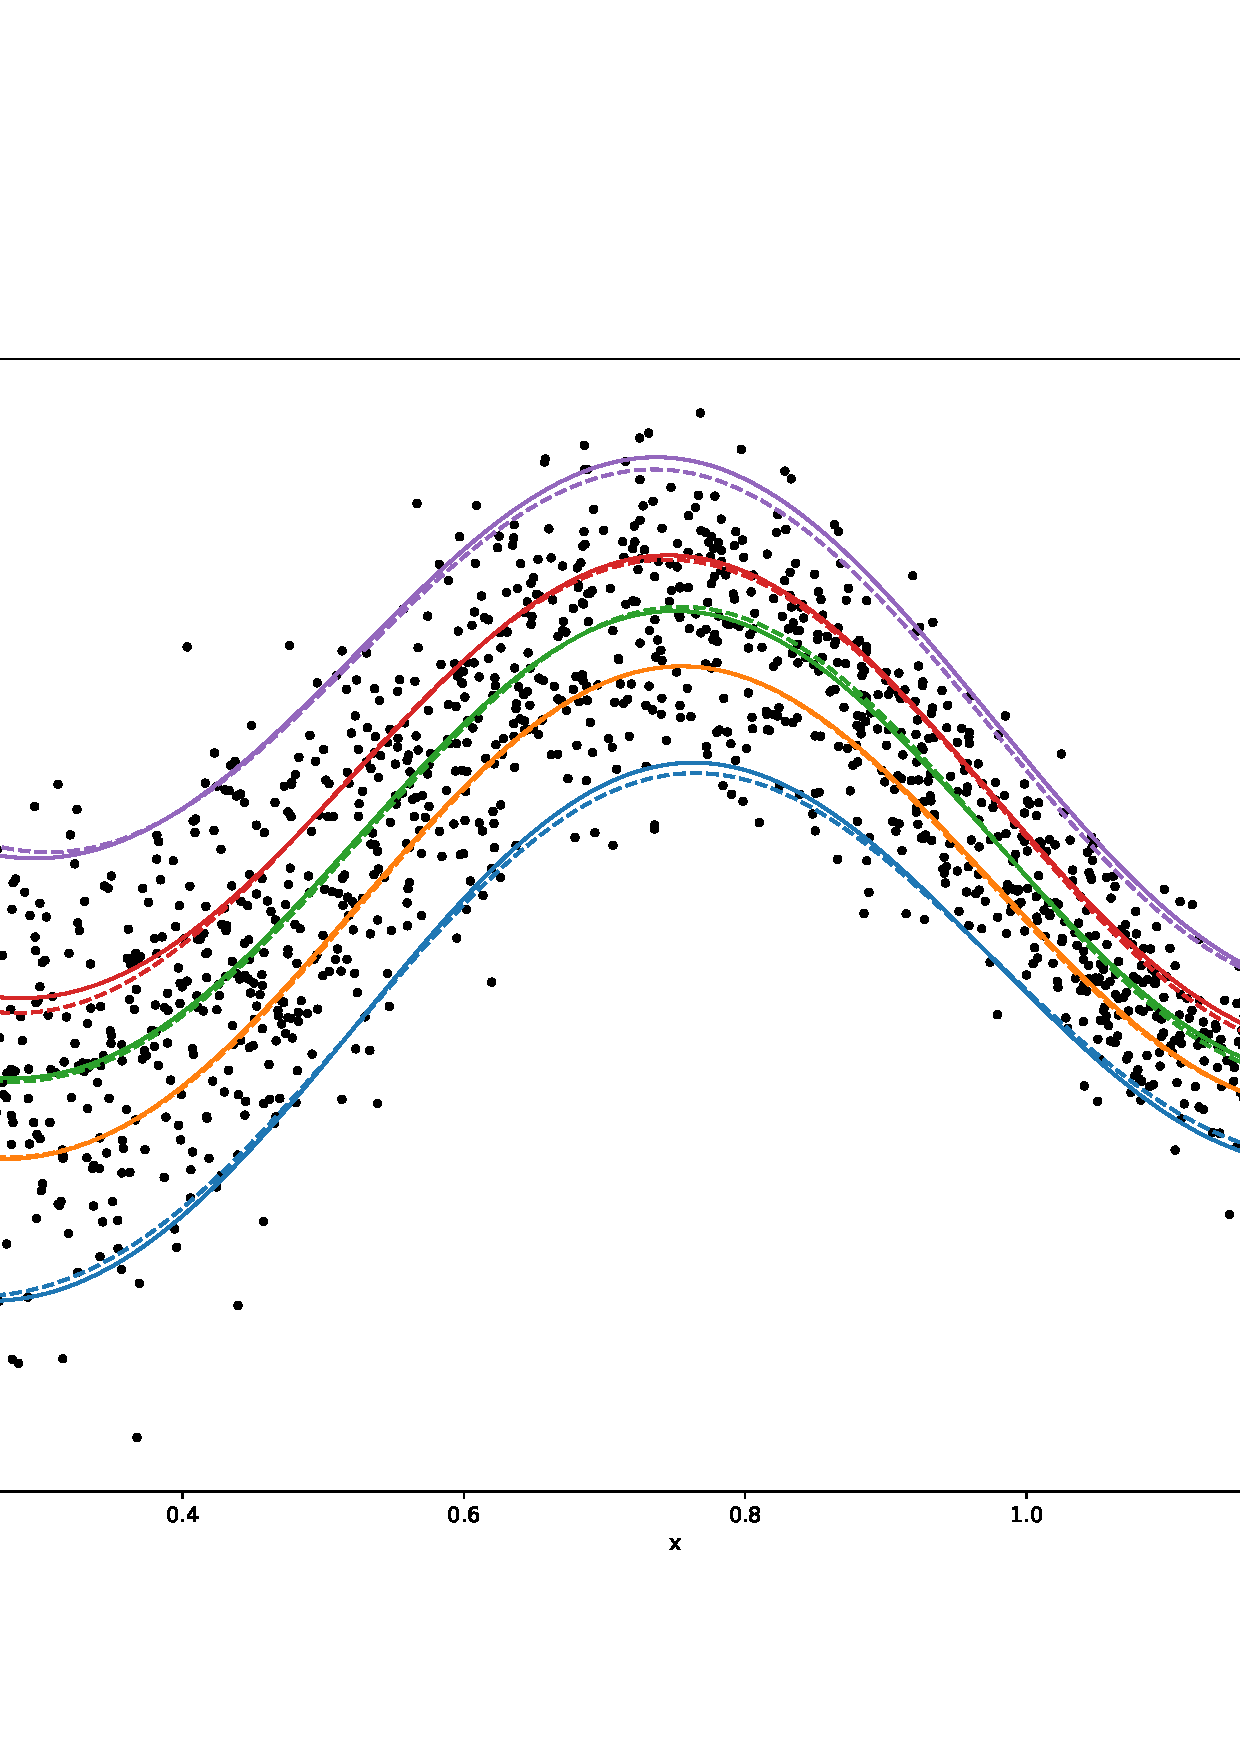
\includegraphics{./gfx/quantile_orff.pdf}}
        %\caption{Learning a continuous quantile function with ORFF
        %regression. \label{fig:quantile_orff}}
    %\end{figure}
    %\clearpage
    %\begin{figure}[htp]
        %\centering\resizebox{.8\textheight}{!}{%
        %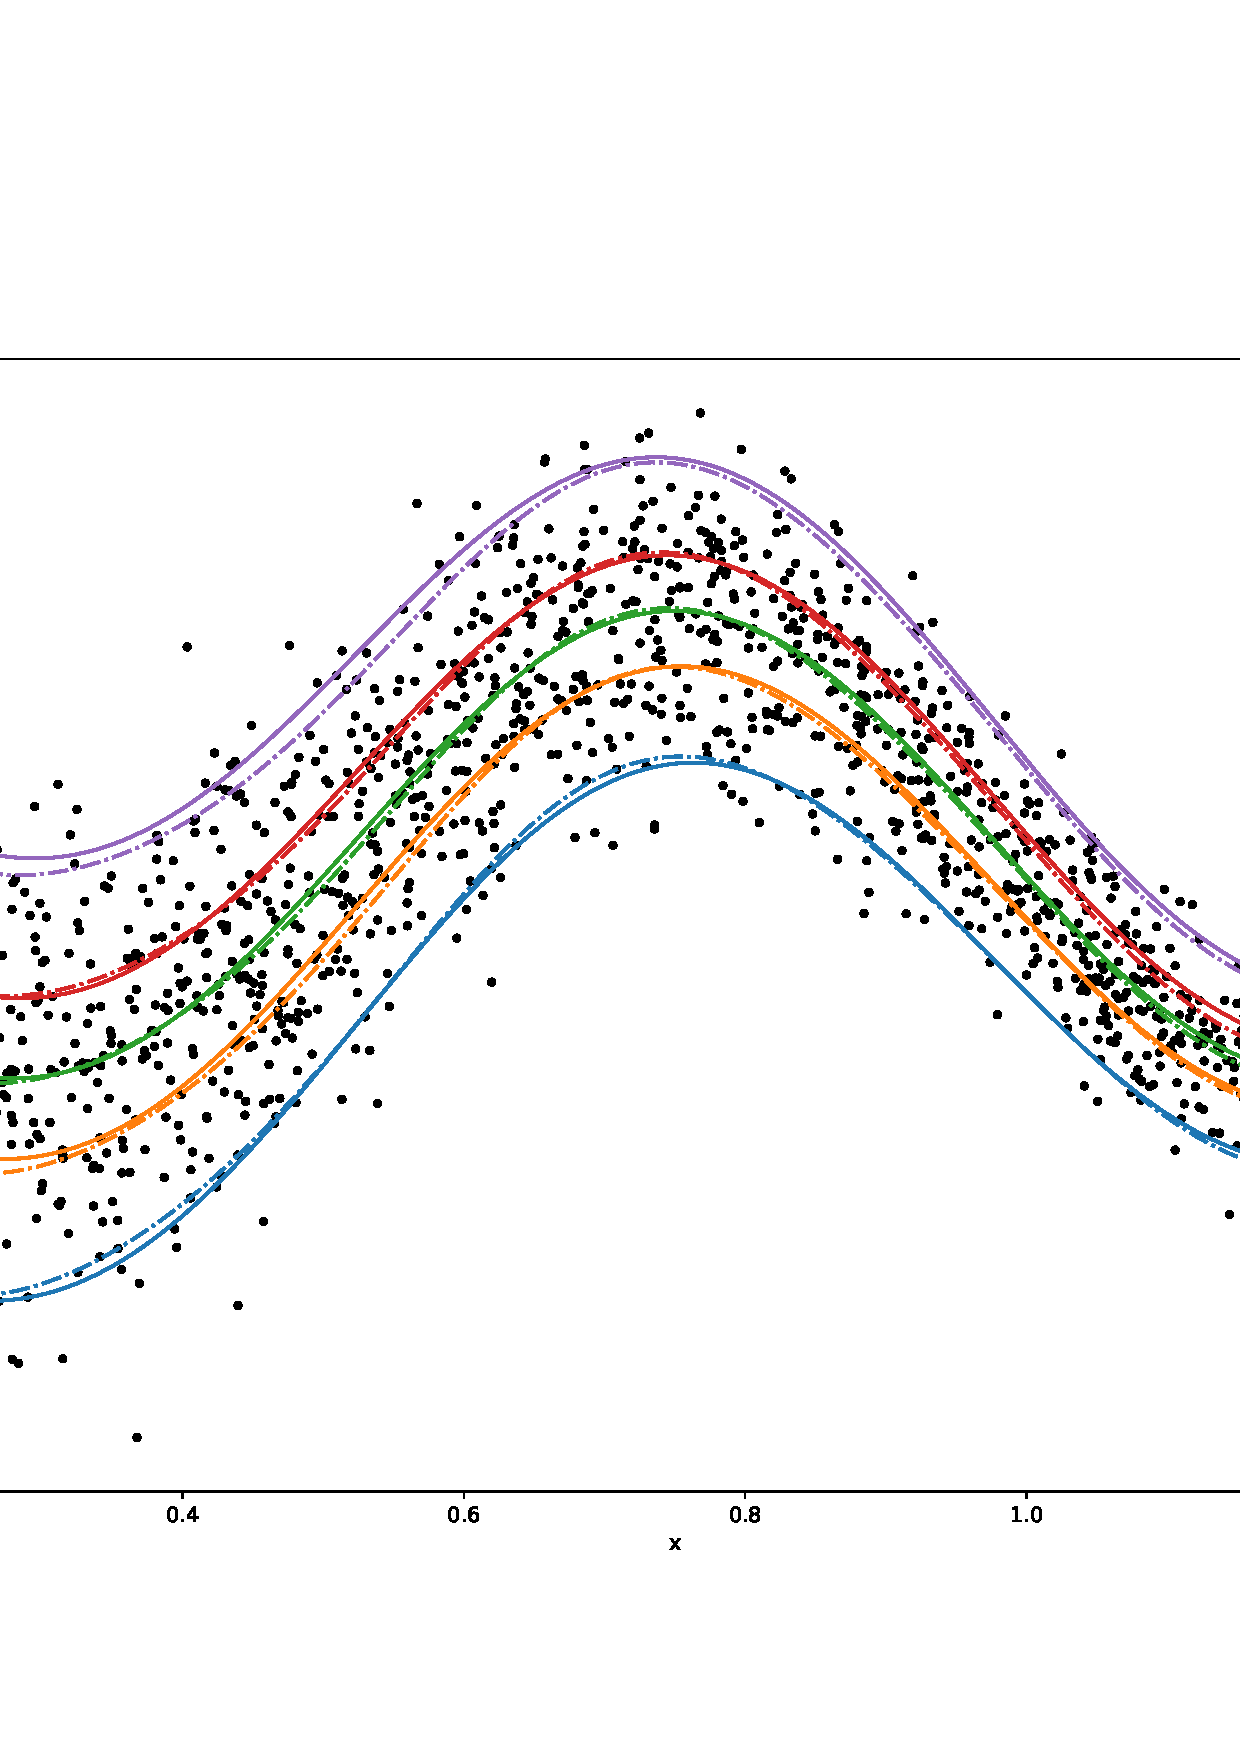
\includegraphics{./gfx/quantile_joint.pdf}}
        %\caption{Learning many quantile with joint OVK regression.
        %\label{fig:quantile_joint}}
    %\end{figure}
%\end{landscape}}
%Moreover $W^\adjoint W$ is the identity on
%$\Ima \Phi_{\tau}$ which is here $\mathcal{H}_{k_{\mathcal{T}}}$. (see the
%proof of \cref{pr:feature_operator} and \citet{Carmeli2010}). Thus we can
%choose $\Phi_\tau=\Phi(\tau)$ to be the functional Fourier feature map
%associated to $k_{\mathcal{T}}$ defined in \cref{pr:fourier_feature_map}.  Then
%we have $BB^\adjoint = I_{\mathcal{H}_{k_{\mathcal{T}}}} = W^\adjoint W$.  Thus
%we can choose $B^\adjoint = W = \Phi(\cdot)^\adjoint$ and the approximate
%feature map reads 
%\begin{dmath*}
    %\tildePhi{\omega}(x)\in \mathcal{L}\left(\mathcal{H}_{k_{\mathcal{T}}};
    %\Vect_{j=1}^D L^2\left(\dual{\mathcal{T}},
    %\probability_{\dual{\Haar},\rho}\right)\right)
%\end{dmath*}
%and
%\begin{dmath*}
    %(\tildePhi{\omega}(x)g)(\tau) = \frac{1}{\sqrt{D}}\Vect_{j=1}^D
    %\begin{pmatrix}
        %\cos(x \omega_j) \Phi(\tau)^\adjoint g \\
        %\sin(x \omega_j) \Phi(\tau)^\adjoint g
    %\end{pmatrix} \condition{$\omega_j \sim \FT{k_{\mathcal{X}}}$
    %\ac{iid}}
%\end{dmath*}
%Then as proposed in \cref{ch:operator-valued_random_fourier_features} we can
%Monte-Carlo sample the functional feature map $\Phi(\tau)$ and obtain the 
%\acs{ORFF} map 
%\begin{dmath*}
    %\left(\widetilde{\tildePhi{\omega}}(x)g\right)(\tau) =
    %\frac{1}{\sqrt{DD'}}\Vect_{j=1}^D
    %\begin{pmatrix}
        %\cos(x \omega_j) \sum_{k=1}^{D'}
        %\left(\cos(\tau \omega_k') + \sin(\tau \omega_k')\right)g(\omega_k') \\
        %\sin(x \omega_j) \sum_{k=1}^{D'}
        %\left(\cos(\tau \omega_k') + \sin(\tau \omega_k')\right)g(\omega_k')
    %\end{pmatrix} \condition{$\omega_j \sim \FT{k_{\mathcal{X}}}$
    %\acs{iid} and $\omega_k'\sim \FT{k_{\mathcal{T}}}$ \acs{iid}.}
%\end{dmath*}
%where $g\in L^2\left(\dual{\mathcal{T}}, \probability_{\dual{\Haar},
%\rho}\right)$ and $\tau\in\mathbb{R}$. If we note 
%\begin{dmath*}
    %G = 
    %\begin{pmatrix}
        %g(\omega_1') & \dots & g(\omega_{D'}') 
    %\end{pmatrix}^\adjoint \hiderel{\in} \mathbb{R}^{D'}
%\end{dmath*}
%we can define
%\begin{dmath*}
    %\left(\widetilde{\tildePhi{\omega}}(x)G\right)(\tau) =
    %\frac{1}{\sqrt{DD'}}\Vect_{j=1}^D
    %\begin{pmatrix}
        %\cos(x \omega_j) \sum_{k=1}^{D'}
        %\left(\cos(\tau \omega_k') + \sin(\tau \omega_k')\right)G_k \\
        %\sin(x \omega_j) \sum_{k=1}^{D'}
        %\left(\cos(\tau \omega_k') + \sin(\tau \omega_k')\right)G_k
    %\end{pmatrix} \condition{$\omega_j \sim \FT{k_{\mathcal{X}}}$
    %\acs{iid} and $\omega_k'\sim \FT{k_{\mathcal{T}}}$ \acs{iid}.}
%\end{dmath*}
%Then it is easy to verify that the adjoint operator is given by
%\begin{dmath*}
    %\left(\widetilde{\tildePhi{\omega}}(x)^\adjoint \theta\right)(\tau) =
    %\frac{1}{\sqrt{DD'}} \sum_{j=1}^D \left(\cos(x\omega_j) +
    %\sin(x\omega_j)\right) \left(\Vect_{k=1}^{D'}
    %\begin{pmatrix}
        %\cos(\tau \omega_k') \\
        %\sin(\tau \omega_k')
    %\end{pmatrix}\right)^\adjoint \theta_j
    %= \frac{1}{\sqrt{DD'}} \sum_{j=1}^D \left(\cos(x\omega_j) +
    %\sin(x\omega_j)\right) \theta_{jk} \left( \cos(\tau \omega_k') + \sin(\tau
    %\omega_k')\right)
    %\condition{$\omega_j \sim \FT{k_{\mathcal{X}}}$
    %\acs{iid} and $\omega_k'\sim \FT{k_{\mathcal{T}}}$ \acs{iid}.}
%\end{dmath*}
%where $\theta_k\in\mathbb{R}^{D'}$, for all $k \in \mathbb{N}^*_D$ and
%$\theta_{jk}\in\mathbb{R}$ for all $j \in \mathbb{N}^*_D$ and all $k \in
%\mathbb{N}^*_{D'}$. The above equations can be rewritten in matrix form which
%results in the following conjecture.
%\begin{conjecture}
    %\label{cj:functional_orff}
    %If $\tildephi{\omega}_{\mathcal{X}}$ is an \acs{RFF} for
    %$\widetilde{k}_{\mathcal{X}}$ such that
    %$\tildephi{\omega}(x)\in\mathbb{R}^D$ and $\tildephi{\omega}_{\mathcal{T}}$
    %is an \acs{RFF} for $\widetilde{k}_{\mathcal{T}}$, such that
    %$\tildephi{\omega}(\tau)\in\mathbb{R}^{D'}$ then an \acs{ORFF} map for
    %\begin{dmath*}
        %K(x, z) = k_{\mathcal{X}}(x, z) I_{\mathcal{H}_{k_{\mathcal{T}}}}
    %\end{dmath*}
    %is given for all $x\in\mathbb{R}$, all $\tau\in\mathbb{R}$ and all
    %$\Theta\in\mathcal{M}_{D,D'}(\mathbb{R})$ by
    %\begin{dmath*}
        %\left(\tildePhi{\omega}_K(x)^\adjoint \Theta \right)(\tau) =
        %\tildephi{\omega}_{\mathcal{X}}(x)^\adjoint \Theta
        %\tildephi{\omega}_{\mathcal{T}}(\tau)
    %\end{dmath*}
    %and
    %\begin{dmath*}
        %\left(\tildePhi{\omega}_K(x) G\right)(\tau) =
        %\tildephi{\omega}_{\mathcal{X}}(x)
        %\tildephi{\omega}_{\mathcal{T}}(\tau)^\adjoint G,
    %\end{dmath*}
    %where $g\in\mathbb{R}^{D'}$.
    %%but more intestingly, given $y\in\mathbb{R}$,
    %%\begin{dmath*}
        %%\tildePhi{\omega}_K(x, \tau)^\adjoint y =
        %%y \tildephi{\omega}_{\mathcal{X}}(x)
        %%\tildephi{\omega}_{\mathcal{T}}(\tau)^\adjoint.
    %%\end{dmath*}
%\end{conjecture}
%Moreover if one defines $\tildePhi{\omega}_K(x,
%\tau) = \left(\tildePhi{\omega}_K(x)^\adjoint \Theta \right)(\tau)$ one
%have of course
%\begin{dmath*}
    %\tildePhi{\omega}_K(x, \tau)^\adjoint \Theta =
    %\tildephi{\omega}_{\mathcal{X}}(x)^\adjoint \Theta
    %\tildephi{\omega}_{\mathcal{T}}(\tau)
%\end{dmath*}
%\subsection{Many quantile regression}
%From the loss defined in \cref{eq:loss_pinball} we defined the regularized risk
%using the \say{continuous} pinball loss for the quantile regression problem.
%For all $f\in\mathcal{H}_K$,
%\begin{dmath*}
    %J_{\lambda}(f) =
    %\frac{1}{N}\sum_{i=1}^N\int_{[0,1]}\left(
    %\begin{cases}
        %\tau\left(f_{x_i}(\tau) - y_i\right) & \text{if } f_{x_i}(\tau) \ge y_i
        %\\
        %(1 - \tau)\left(y_i - f_{x_i}(\tau)\right) & \text{otherwise} 
    %\end{cases} \right)+ \lambda
    %\norm{f}_K^2.
%\end{dmath*}
%The issue with the above risk is that the different quantile for a given point
%$x\in\mathbb{R}$ may cross \citet{sangnier2016joint}. To avoid this to happen
%we need to force the function $f_x(\tau)$ to be \emph{increasing} in $\tau$ for
%any $x\in\mathbb{R}$.  Because a decreasing function has a negative derivative
%we can add a penalty term to the risk to avoid $f_x(\tau)$ to be decreasing in
%$\tau$.
%\begin{dmath*}
    %\Omega_{cross}(f) = - \min\left(\frac{\partial
    %f_{x_i}}{\partial\tau}(\tau),
    %0\right)
%\end{dmath*}
%Thus the regularized risk with the no crossing constraint is
%\begin{dmath*}
    %J_{\lambda_1, \lambda_2}(f) =
    %\frac{1}{N}\sum_{i=1}^N\int_{[0,1]}\left(
    %\begin{cases} 
        %\tau \left(f_{x_i}(\tau) - y_i\right) & \text{if } f_{x_i}(\tau) \ge
        %y_i \\
        %(1 - \tau)\left(y_i - f_{x_i}(\tau)\right) & \text{otherwise}
    %\end{cases} -
    %\lambda_1 \min\left(\frac{\partial f_{x_i}}{\partial\tau}(\tau), 0\right)
    %\right)+ \lambda_2 \norm{f}_K^2.
%\end{dmath*}
%Eventually we replace the integral by a Monte-Carlo sampling with the uniform
%law $\mathcal{U}([0, 1])$ and plug in the approximate function of $f$ using the
%\acs{ORFF} map proposed in \cref{cj:functional_orff}. The final optimzation
%problem reads
%\begin{dmath*}
    %J_{\lambda_1, \lambda_2}(\Theta) =
    %\frac{1}{NT}\sum_{i=1}^N\sum_{t=1}^T\left(
    %\begin{cases} \tau_t
        %\left(\widetilde{f}_{x_i}(\tau_t) - y_i\right) & \text{if }
        %\widetilde{f}_{x_i}(\tau_t) \ge y_i \\
        %(1 - \tau_t)\left(y_i - f_{x_i}(\tau_t)\right) & \text{otherwise} 
    %\end{cases} - \lambda_1
    %\min\left(\frac{\partial \widetilde{f}_{x_i}}{\partial\tau}(\tau_t),
    %0\right) \right)+ \lambda_2 \norm{\Theta}_{fro}^2.
%\end{dmath*}
%where $\widetilde{f}_{x}(\tau)=\tildephi{\omega}_{\mathcal{X}}(x)^\adjoint
%\Theta \tildephi{\omega}_{\mathcal{T}}(\tau)$, $\tau_t \sim \mathcal{U}([0,
%1])$ and
%\begin{dmath*}
    %\frac{\partial \widetilde{f}_{x}}{\partial\tau}(\tau)
    %= \tildephi{\omega}_{\mathcal{X}}(x)^\adjoint \Theta \frac{\partial
    %\tildephi{\omega}_{\mathcal{T}}}{\partial \tau}(\tau)
    %= \tildephi{\omega}_{\mathcal{X}}(x)^\adjoint \Theta \Vect_{k=1}^{D'}
    %\begin{pmatrix}
        %-\omega_k' \sin(\omega_k' x) \\
         %\omega_k' \cos(\omega_k' x)
    %\end{pmatrix} \condition{$\omega_k' \sim \FT{k_{\mathcal{T}}}$ \acs{iid}.}
%\end{dmath*}
%\subsubsection{Some results}
%We minimize the quantity $J_{\lambda_1, \lambda_2}(\Theta)$ on a toy dataset: a
%sine wave with some heteroscedastic noise. First we compare our methodology to
%the joint quantile regression proposed in \citet{sangnier2016joint}. We
%generate $N=2500$ for the train set and $N'=1000$ points for the test set and
%use a gaussian kernel for both $k_{\mathcal{X}}$ and $k_{\mathcal{T}}$. We
%choosed $\sigma_{\mathcal{X}} = 0.25$ and $\sigma_{\mathcal{T}}$ is set to be
%the median of the pairwise distance of the $\tau_t$'s drawn randomly from
%$\mathcal{U}([0, 1])$. Notice that $J_{\lambda_1, \lambda_2}(\Theta)$ is convex
%in $\Theta$. To avoid computing complex gradients and by lack of time, we used
%Tensorflow \citep{abadi2016tensorflow} to perform a gradient descent (with
%RMSProp \citep{tieleman2012lecture}) with automatic symbolic differentiation.
%\Cref{fig:quantile_orff} show the result for the quantile at $0.05$, $0.275$,
%$0.5$, $0.775$ and $0.95$ using the \acs{ORFF} methodology. 
%\afterpage{%
%\begin{landscape}
    %\begin{figure}[htp]
        %\centering
        %\resizebox{.8\textheight}{!}{%
        %\includegraphics{./gfx/quantile_continuous.pgf}}
        %\caption{Learning a continuous quantile function with ORFF
        %regression. \label{fig:quantile_continuous}}
    %\end{figure}
%\end{landscape}}
%\Cref{fig:quantile_joint} shows the joint quantile regression of
%\citet{sangnier2016joint} on the same dataset. Not only our method matches the
%the performances of \citet{sangnier2016joint}\footnote{We reported an error
%computed with the pinball loss on the test set of $0.818$ for our method and
%$0.817$ for joint regression (note that we don't report here an average on many
%experiments to avoid randomness introduced by the random features, but the
%results seems robut in practice.)} but we cut down the computation time from
%circa $1330$ seconds to circa $30$ seconds (training and testing).  Moreover on
%contrary to \citet{sangnier2016joint} we have access to all the quantile of the
%model (see \cref{fig:quantile_continuous}).

%\subsection{One class SVM revisited}
%We also propose an extension of the celebrated \acf{OCSVM} so that it
%possible to learn jointly all the level sets.  One-class classification, also
%known as unary classification, tries to identify objects of a specific class
%amongst all objects, by learning from a training set containing only the
%objects of that class.  In this framework, we assume that we only observe
%examples of one class (referred to as the inlier class).  The second class is
%called outlier class.  We turn our attention to the \acs{OCSVM}
%of \citet{Scholkopf2001} which extends the \ac{SVM} methodology
%\citep{Cortes1995,Shawe2004} to handle training using only inliers. 
%\paragraph{}
%We recall that given an hyperparameter $\nu\in [0,1]$ that controls the
%proportion of inlier, given as scalar kernel $k$, the \acs{OCSVM} problem reads
%\begin{dmath*}
    %\argmin_{f\in\mathcal{H}_k, \tau \in \mathbb{R}} \frac{1}{2}
    %\norm{f}_{\mathcal{H}_k}^2 - \nu \tau + \frac{1}{N} \sum_{i=1}^N \max(\tau
    %- f(x_i), 0)
%\end{dmath*}
%The decision function is then
%\begin{dmath*}
    %h(x, \tau) = \mathds{1}_{[\tau, \infty)}\left( f(x) \right).
%\end{dmath*}
%As in \cref{subsec:quantile_regression} we can rewrite the optimization problem
%as an integral over all the value of $\nu$ and suppose that $f$ is
%function-valued (a function of $\nu$). Moreover $\tau$ must also change its
%value according to $\mu$. Thus given a kernel $k_{\mathcal{X}}$ on the inputs
%$x\in\mathbb{R}^d$ with its approximate feature map
%$\tildephi{\omega}_{\mathcal{X}}$ and a kernel $k_{\mathcal{T}}$ on the level
%sets with its approximate feature map $\tildephi{\omega}_{\mathcal{T}}$, we
%define the continuous one-class SVM problem as
%\begin{dmath*}
    %\argmin_{f
    %\in\mathcal{H}_K,\tau\in\mathcal{H}_{k_{\mathcal{\tau}}}}\frac{1}{N}
    %\sum_{i=1}^N\int_{[0,1]}\max\left(0, \tau(\nu) - f_{x_i}(\nu)\right)d\nu +
    %\frac{1}{2}\int_{[0,1]}\nu
    %\norm{f_{\cdot}(\nu)}_{\mathcal{H}_{k_{\mathcal{X}}}}^2d\nu -
    %\int_{[0,1]}\nu\tau(\nu)d\nu.
%\end{dmath*}
%Again we can compute the integral by Monte-Carlo sampling and replace $f$ and
%$\tau$ by their respective approximation. Notice that the \acs{RKHS} of $\tau$
%should match the \acs{RKHS} of the output space of $f_K$. Hence
%\begin{dmath*}
    %\argmin_{\Theta
    %\in\mathcal{M}_{D, D'}(\mathbb{R}),\tau\in\mathbb{R}^D}\frac{1}{NT}
    %\sum_{i=1}^N\sum_{t=1}^T\max\left(0, \widetilde{\tau}(\nu_t) -
    %\widetilde{f}_{x_i}(\nu_t)\right) + \frac{1}{2T}\sum_{t=1}^T\nu_t
    %\norm{\widetilde{f}_{\cdot}(\nu_t)}_{2}^2 -
    %\frac{1}{T}\sum_{t=1}^T\nu_t\widetilde{\tau}(\nu_t),
%\end{dmath*}
%where $\nu_t \sim \mathcal{U}([0, 1])$ \acs{iid}, $\widetilde{\tau}(\nu) =
%\tildephi{\omega}_{\mathcal{T}}(\nu)$ and $\widetilde{f}_x(\nu) =
%\tildephi{\omega}(x)^\adjoint \Theta \tildephi{\omega}_{\mathcal{T}}(\nu)$. We
%also deduce that $\widetilde{f}_{\cdot}(\nu) = \Theta
%\tildephi{\omega}_{\mathcal{T}}(\nu)$. Here the natural decision function is
%\begin{dmath}
    %\label{eq:continuous_decision}
    %h(x, \nu) = \mathds{1}_{\left[\widetilde{\tau}(\nu),\infty\right)}
    %\left(\widetilde{f}_x(\nu)\right).
%\end{dmath}
%\begin{figure}
    %{\centering
    %\resizebox{2\textwidth}{!}{%% Creator: Matplotlib, PGF backend
%%
%% To include the figure in your LaTeX document, write
%%   \input{<filename>.pgf}
%%
%% Make sure the required packages are loaded in your preamble
%%   \usepackage{pgf}
%%
%% Figures using additional raster images can only be included by \input if
%% they are in the same directory as the main LaTeX file. For loading figures
%% from other directories you can use the `import` package
%%   \usepackage{import}
%% and then include the figures with
%%   \import{<path to file>}{<filename>.pgf}
%%
%% Matplotlib used the following preamble
%%   \usepackage{fontspec}
%%   \setmainfont{Times New Roman}
%%   \setsansfont{Lucida Grande}
%%   \setmonofont{Andale Mono}
%%
\begingroup%
\makeatletter%
\begin{pgfpicture}%
\pgfpathrectangle{\pgfpointorigin}{\pgfqpoint{16.000000in}{5.000000in}}%
\pgfusepath{use as bounding box, clip}%
\begin{pgfscope}%
\pgfsetbuttcap%
\pgfsetmiterjoin%
\definecolor{currentfill}{rgb}{1.000000,1.000000,1.000000}%
\pgfsetfillcolor{currentfill}%
\pgfsetlinewidth{0.000000pt}%
\definecolor{currentstroke}{rgb}{1.000000,1.000000,1.000000}%
\pgfsetstrokecolor{currentstroke}%
\pgfsetdash{}{0pt}%
\pgfpathmoveto{\pgfqpoint{0.000000in}{0.000000in}}%
\pgfpathlineto{\pgfqpoint{16.000000in}{0.000000in}}%
\pgfpathlineto{\pgfqpoint{16.000000in}{5.000000in}}%
\pgfpathlineto{\pgfqpoint{0.000000in}{5.000000in}}%
\pgfpathclose%
\pgfusepath{fill}%
\end{pgfscope}%
\begin{pgfscope}%
\pgfsetbuttcap%
\pgfsetmiterjoin%
\definecolor{currentfill}{rgb}{1.000000,1.000000,1.000000}%
\pgfsetfillcolor{currentfill}%
\pgfsetlinewidth{0.000000pt}%
\definecolor{currentstroke}{rgb}{0.000000,0.000000,0.000000}%
\pgfsetstrokecolor{currentstroke}%
\pgfsetstrokeopacity{0.000000}%
\pgfsetdash{}{0pt}%
\pgfpathmoveto{\pgfqpoint{0.663889in}{0.580556in}}%
\pgfpathlineto{\pgfqpoint{8.157639in}{0.580556in}}%
\pgfpathlineto{\pgfqpoint{8.157639in}{4.801389in}}%
\pgfpathlineto{\pgfqpoint{0.663889in}{4.801389in}}%
\pgfpathclose%
\pgfusepath{fill}%
\end{pgfscope}%
\begin{pgfscope}%
\pgfsetbuttcap%
\pgfsetroundjoin%
\definecolor{currentfill}{rgb}{0.000000,0.000000,0.000000}%
\pgfsetfillcolor{currentfill}%
\pgfsetlinewidth{0.803000pt}%
\definecolor{currentstroke}{rgb}{0.000000,0.000000,0.000000}%
\pgfsetstrokecolor{currentstroke}%
\pgfsetdash{}{0pt}%
\pgfsys@defobject{currentmarker}{\pgfqpoint{0.000000in}{-0.048611in}}{\pgfqpoint{0.000000in}{0.000000in}}{%
\pgfpathmoveto{\pgfqpoint{0.000000in}{0.000000in}}%
\pgfpathlineto{\pgfqpoint{0.000000in}{-0.048611in}}%
\pgfusepath{stroke,fill}%
}%
\begin{pgfscope}%
\pgfsys@transformshift{1.004514in}{0.580556in}%
\pgfsys@useobject{currentmarker}{}%
\end{pgfscope}%
\end{pgfscope}%
\begin{pgfscope}%
\pgftext[x=1.004514in,y=0.483333in,,top]{\sffamily\fontsize{10.000000}{12.000000}\selectfont 0.0}%
\end{pgfscope}%
\begin{pgfscope}%
\pgfsetbuttcap%
\pgfsetroundjoin%
\definecolor{currentfill}{rgb}{0.000000,0.000000,0.000000}%
\pgfsetfillcolor{currentfill}%
\pgfsetlinewidth{0.803000pt}%
\definecolor{currentstroke}{rgb}{0.000000,0.000000,0.000000}%
\pgfsetstrokecolor{currentstroke}%
\pgfsetdash{}{0pt}%
\pgfsys@defobject{currentmarker}{\pgfqpoint{0.000000in}{-0.048611in}}{\pgfqpoint{0.000000in}{0.000000in}}{%
\pgfpathmoveto{\pgfqpoint{0.000000in}{0.000000in}}%
\pgfpathlineto{\pgfqpoint{0.000000in}{-0.048611in}}%
\pgfusepath{stroke,fill}%
}%
\begin{pgfscope}%
\pgfsys@transformshift{2.367014in}{0.580556in}%
\pgfsys@useobject{currentmarker}{}%
\end{pgfscope}%
\end{pgfscope}%
\begin{pgfscope}%
\pgftext[x=2.367014in,y=0.483333in,,top]{\sffamily\fontsize{10.000000}{12.000000}\selectfont 0.2}%
\end{pgfscope}%
\begin{pgfscope}%
\pgfsetbuttcap%
\pgfsetroundjoin%
\definecolor{currentfill}{rgb}{0.000000,0.000000,0.000000}%
\pgfsetfillcolor{currentfill}%
\pgfsetlinewidth{0.803000pt}%
\definecolor{currentstroke}{rgb}{0.000000,0.000000,0.000000}%
\pgfsetstrokecolor{currentstroke}%
\pgfsetdash{}{0pt}%
\pgfsys@defobject{currentmarker}{\pgfqpoint{0.000000in}{-0.048611in}}{\pgfqpoint{0.000000in}{0.000000in}}{%
\pgfpathmoveto{\pgfqpoint{0.000000in}{0.000000in}}%
\pgfpathlineto{\pgfqpoint{0.000000in}{-0.048611in}}%
\pgfusepath{stroke,fill}%
}%
\begin{pgfscope}%
\pgfsys@transformshift{3.729514in}{0.580556in}%
\pgfsys@useobject{currentmarker}{}%
\end{pgfscope}%
\end{pgfscope}%
\begin{pgfscope}%
\pgftext[x=3.729514in,y=0.483333in,,top]{\sffamily\fontsize{10.000000}{12.000000}\selectfont 0.4}%
\end{pgfscope}%
\begin{pgfscope}%
\pgfsetbuttcap%
\pgfsetroundjoin%
\definecolor{currentfill}{rgb}{0.000000,0.000000,0.000000}%
\pgfsetfillcolor{currentfill}%
\pgfsetlinewidth{0.803000pt}%
\definecolor{currentstroke}{rgb}{0.000000,0.000000,0.000000}%
\pgfsetstrokecolor{currentstroke}%
\pgfsetdash{}{0pt}%
\pgfsys@defobject{currentmarker}{\pgfqpoint{0.000000in}{-0.048611in}}{\pgfqpoint{0.000000in}{0.000000in}}{%
\pgfpathmoveto{\pgfqpoint{0.000000in}{0.000000in}}%
\pgfpathlineto{\pgfqpoint{0.000000in}{-0.048611in}}%
\pgfusepath{stroke,fill}%
}%
\begin{pgfscope}%
\pgfsys@transformshift{5.092014in}{0.580556in}%
\pgfsys@useobject{currentmarker}{}%
\end{pgfscope}%
\end{pgfscope}%
\begin{pgfscope}%
\pgftext[x=5.092014in,y=0.483333in,,top]{\sffamily\fontsize{10.000000}{12.000000}\selectfont 0.6}%
\end{pgfscope}%
\begin{pgfscope}%
\pgfsetbuttcap%
\pgfsetroundjoin%
\definecolor{currentfill}{rgb}{0.000000,0.000000,0.000000}%
\pgfsetfillcolor{currentfill}%
\pgfsetlinewidth{0.803000pt}%
\definecolor{currentstroke}{rgb}{0.000000,0.000000,0.000000}%
\pgfsetstrokecolor{currentstroke}%
\pgfsetdash{}{0pt}%
\pgfsys@defobject{currentmarker}{\pgfqpoint{0.000000in}{-0.048611in}}{\pgfqpoint{0.000000in}{0.000000in}}{%
\pgfpathmoveto{\pgfqpoint{0.000000in}{0.000000in}}%
\pgfpathlineto{\pgfqpoint{0.000000in}{-0.048611in}}%
\pgfusepath{stroke,fill}%
}%
\begin{pgfscope}%
\pgfsys@transformshift{6.454514in}{0.580556in}%
\pgfsys@useobject{currentmarker}{}%
\end{pgfscope}%
\end{pgfscope}%
\begin{pgfscope}%
\pgftext[x=6.454514in,y=0.483333in,,top]{\sffamily\fontsize{10.000000}{12.000000}\selectfont 0.8}%
\end{pgfscope}%
\begin{pgfscope}%
\pgfsetbuttcap%
\pgfsetroundjoin%
\definecolor{currentfill}{rgb}{0.000000,0.000000,0.000000}%
\pgfsetfillcolor{currentfill}%
\pgfsetlinewidth{0.803000pt}%
\definecolor{currentstroke}{rgb}{0.000000,0.000000,0.000000}%
\pgfsetstrokecolor{currentstroke}%
\pgfsetdash{}{0pt}%
\pgfsys@defobject{currentmarker}{\pgfqpoint{0.000000in}{-0.048611in}}{\pgfqpoint{0.000000in}{0.000000in}}{%
\pgfpathmoveto{\pgfqpoint{0.000000in}{0.000000in}}%
\pgfpathlineto{\pgfqpoint{0.000000in}{-0.048611in}}%
\pgfusepath{stroke,fill}%
}%
\begin{pgfscope}%
\pgfsys@transformshift{7.817014in}{0.580556in}%
\pgfsys@useobject{currentmarker}{}%
\end{pgfscope}%
\end{pgfscope}%
\begin{pgfscope}%
\pgftext[x=7.817014in,y=0.483333in,,top]{\sffamily\fontsize{10.000000}{12.000000}\selectfont 1.0}%
\end{pgfscope}%
\begin{pgfscope}%
\pgftext[x=4.410764in,y=0.293908in,,top]{\sffamily\fontsize{10.000000}{12.000000}\selectfont \(\displaystyle \nu\)}%
\end{pgfscope}%
\begin{pgfscope}%
\pgfsetbuttcap%
\pgfsetroundjoin%
\definecolor{currentfill}{rgb}{0.000000,0.000000,0.000000}%
\pgfsetfillcolor{currentfill}%
\pgfsetlinewidth{0.803000pt}%
\definecolor{currentstroke}{rgb}{0.000000,0.000000,0.000000}%
\pgfsetstrokecolor{currentstroke}%
\pgfsetdash{}{0pt}%
\pgfsys@defobject{currentmarker}{\pgfqpoint{-0.048611in}{0.000000in}}{\pgfqpoint{0.000000in}{0.000000in}}{%
\pgfpathmoveto{\pgfqpoint{0.000000in}{0.000000in}}%
\pgfpathlineto{\pgfqpoint{-0.048611in}{0.000000in}}%
\pgfusepath{stroke,fill}%
}%
\begin{pgfscope}%
\pgfsys@transformshift{0.663889in}{0.772412in}%
\pgfsys@useobject{currentmarker}{}%
\end{pgfscope}%
\end{pgfscope}%
\begin{pgfscope}%
\pgftext[x=0.347076in,y=0.718870in,left,base]{\sffamily\fontsize{10.000000}{12.000000}\selectfont 0.0}%
\end{pgfscope}%
\begin{pgfscope}%
\pgfsetbuttcap%
\pgfsetroundjoin%
\definecolor{currentfill}{rgb}{0.000000,0.000000,0.000000}%
\pgfsetfillcolor{currentfill}%
\pgfsetlinewidth{0.803000pt}%
\definecolor{currentstroke}{rgb}{0.000000,0.000000,0.000000}%
\pgfsetstrokecolor{currentstroke}%
\pgfsetdash{}{0pt}%
\pgfsys@defobject{currentmarker}{\pgfqpoint{-0.048611in}{0.000000in}}{\pgfqpoint{0.000000in}{0.000000in}}{%
\pgfpathmoveto{\pgfqpoint{0.000000in}{0.000000in}}%
\pgfpathlineto{\pgfqpoint{-0.048611in}{0.000000in}}%
\pgfusepath{stroke,fill}%
}%
\begin{pgfscope}%
\pgfsys@transformshift{0.663889in}{1.539836in}%
\pgfsys@useobject{currentmarker}{}%
\end{pgfscope}%
\end{pgfscope}%
\begin{pgfscope}%
\pgftext[x=0.347076in,y=1.486294in,left,base]{\sffamily\fontsize{10.000000}{12.000000}\selectfont 0.2}%
\end{pgfscope}%
\begin{pgfscope}%
\pgfsetbuttcap%
\pgfsetroundjoin%
\definecolor{currentfill}{rgb}{0.000000,0.000000,0.000000}%
\pgfsetfillcolor{currentfill}%
\pgfsetlinewidth{0.803000pt}%
\definecolor{currentstroke}{rgb}{0.000000,0.000000,0.000000}%
\pgfsetstrokecolor{currentstroke}%
\pgfsetdash{}{0pt}%
\pgfsys@defobject{currentmarker}{\pgfqpoint{-0.048611in}{0.000000in}}{\pgfqpoint{0.000000in}{0.000000in}}{%
\pgfpathmoveto{\pgfqpoint{0.000000in}{0.000000in}}%
\pgfpathlineto{\pgfqpoint{-0.048611in}{0.000000in}}%
\pgfusepath{stroke,fill}%
}%
\begin{pgfscope}%
\pgfsys@transformshift{0.663889in}{2.307260in}%
\pgfsys@useobject{currentmarker}{}%
\end{pgfscope}%
\end{pgfscope}%
\begin{pgfscope}%
\pgftext[x=0.347076in,y=2.253719in,left,base]{\sffamily\fontsize{10.000000}{12.000000}\selectfont 0.4}%
\end{pgfscope}%
\begin{pgfscope}%
\pgfsetbuttcap%
\pgfsetroundjoin%
\definecolor{currentfill}{rgb}{0.000000,0.000000,0.000000}%
\pgfsetfillcolor{currentfill}%
\pgfsetlinewidth{0.803000pt}%
\definecolor{currentstroke}{rgb}{0.000000,0.000000,0.000000}%
\pgfsetstrokecolor{currentstroke}%
\pgfsetdash{}{0pt}%
\pgfsys@defobject{currentmarker}{\pgfqpoint{-0.048611in}{0.000000in}}{\pgfqpoint{0.000000in}{0.000000in}}{%
\pgfpathmoveto{\pgfqpoint{0.000000in}{0.000000in}}%
\pgfpathlineto{\pgfqpoint{-0.048611in}{0.000000in}}%
\pgfusepath{stroke,fill}%
}%
\begin{pgfscope}%
\pgfsys@transformshift{0.663889in}{3.074684in}%
\pgfsys@useobject{currentmarker}{}%
\end{pgfscope}%
\end{pgfscope}%
\begin{pgfscope}%
\pgftext[x=0.347076in,y=3.021143in,left,base]{\sffamily\fontsize{10.000000}{12.000000}\selectfont 0.6}%
\end{pgfscope}%
\begin{pgfscope}%
\pgfsetbuttcap%
\pgfsetroundjoin%
\definecolor{currentfill}{rgb}{0.000000,0.000000,0.000000}%
\pgfsetfillcolor{currentfill}%
\pgfsetlinewidth{0.803000pt}%
\definecolor{currentstroke}{rgb}{0.000000,0.000000,0.000000}%
\pgfsetstrokecolor{currentstroke}%
\pgfsetdash{}{0pt}%
\pgfsys@defobject{currentmarker}{\pgfqpoint{-0.048611in}{0.000000in}}{\pgfqpoint{0.000000in}{0.000000in}}{%
\pgfpathmoveto{\pgfqpoint{0.000000in}{0.000000in}}%
\pgfpathlineto{\pgfqpoint{-0.048611in}{0.000000in}}%
\pgfusepath{stroke,fill}%
}%
\begin{pgfscope}%
\pgfsys@transformshift{0.663889in}{3.842109in}%
\pgfsys@useobject{currentmarker}{}%
\end{pgfscope}%
\end{pgfscope}%
\begin{pgfscope}%
\pgftext[x=0.347076in,y=3.788567in,left,base]{\sffamily\fontsize{10.000000}{12.000000}\selectfont 0.8}%
\end{pgfscope}%
\begin{pgfscope}%
\pgfsetbuttcap%
\pgfsetroundjoin%
\definecolor{currentfill}{rgb}{0.000000,0.000000,0.000000}%
\pgfsetfillcolor{currentfill}%
\pgfsetlinewidth{0.803000pt}%
\definecolor{currentstroke}{rgb}{0.000000,0.000000,0.000000}%
\pgfsetstrokecolor{currentstroke}%
\pgfsetdash{}{0pt}%
\pgfsys@defobject{currentmarker}{\pgfqpoint{-0.048611in}{0.000000in}}{\pgfqpoint{0.000000in}{0.000000in}}{%
\pgfpathmoveto{\pgfqpoint{0.000000in}{0.000000in}}%
\pgfpathlineto{\pgfqpoint{-0.048611in}{0.000000in}}%
\pgfusepath{stroke,fill}%
}%
\begin{pgfscope}%
\pgfsys@transformshift{0.663889in}{4.609533in}%
\pgfsys@useobject{currentmarker}{}%
\end{pgfscope}%
\end{pgfscope}%
\begin{pgfscope}%
\pgftext[x=0.347076in,y=4.555991in,left,base]{\sffamily\fontsize{10.000000}{12.000000}\selectfont 1.0}%
\end{pgfscope}%
\begin{pgfscope}%
\pgftext[x=0.291520in,y=2.690972in,,bottom,rotate=90.000000]{\sffamily\fontsize{10.000000}{12.000000}\selectfont percentage of inliers}%
\end{pgfscope}%
\begin{pgfscope}%
\pgfpathrectangle{\pgfqpoint{0.663889in}{0.580556in}}{\pgfqpoint{7.493750in}{4.220833in}} %
\pgfusepath{clip}%
\pgfsetrectcap%
\pgfsetroundjoin%
\pgfsetlinewidth{1.505625pt}%
\definecolor{currentstroke}{rgb}{0.121569,0.466667,0.705882}%
\pgfsetstrokecolor{currentstroke}%
\pgfsetdash{}{0pt}%
\pgfpathmoveto{\pgfqpoint{1.004514in}{4.099744in}}%
\pgfpathlineto{\pgfqpoint{1.073327in}{4.181968in}}%
\pgfpathlineto{\pgfqpoint{1.142140in}{4.072336in}}%
\pgfpathlineto{\pgfqpoint{1.210953in}{4.006557in}}%
\pgfpathlineto{\pgfqpoint{1.279766in}{3.979149in}}%
\pgfpathlineto{\pgfqpoint{1.348580in}{3.973667in}}%
\pgfpathlineto{\pgfqpoint{1.417393in}{3.951741in}}%
\pgfpathlineto{\pgfqpoint{1.486206in}{3.918851in}}%
\pgfpathlineto{\pgfqpoint{1.555019in}{3.842109in}}%
\pgfpathlineto{\pgfqpoint{1.623832in}{3.820182in}}%
\pgfpathlineto{\pgfqpoint{1.692645in}{3.787293in}}%
\pgfpathlineto{\pgfqpoint{1.761458in}{3.743440in}}%
\pgfpathlineto{\pgfqpoint{1.830271in}{3.710550in}}%
\pgfpathlineto{\pgfqpoint{1.899085in}{3.672179in}}%
\pgfpathlineto{\pgfqpoint{1.967898in}{3.633808in}}%
\pgfpathlineto{\pgfqpoint{2.036711in}{3.595437in}}%
\pgfpathlineto{\pgfqpoint{2.105524in}{3.578992in}}%
\pgfpathlineto{\pgfqpoint{2.174337in}{3.557065in}}%
\pgfpathlineto{\pgfqpoint{2.243150in}{3.480323in}}%
\pgfpathlineto{\pgfqpoint{2.311963in}{3.436470in}}%
\pgfpathlineto{\pgfqpoint{2.380777in}{3.425507in}}%
\pgfpathlineto{\pgfqpoint{2.449590in}{3.398099in}}%
\pgfpathlineto{\pgfqpoint{2.518403in}{3.354246in}}%
\pgfpathlineto{\pgfqpoint{2.587216in}{3.321356in}}%
\pgfpathlineto{\pgfqpoint{2.656029in}{3.293948in}}%
\pgfpathlineto{\pgfqpoint{2.724842in}{3.272022in}}%
\pgfpathlineto{\pgfqpoint{2.793655in}{3.244614in}}%
\pgfpathlineto{\pgfqpoint{2.862468in}{3.206243in}}%
\pgfpathlineto{\pgfqpoint{2.931282in}{3.140464in}}%
\pgfpathlineto{\pgfqpoint{3.000095in}{3.107574in}}%
\pgfpathlineto{\pgfqpoint{3.068908in}{3.080166in}}%
\pgfpathlineto{\pgfqpoint{3.137721in}{3.058240in}}%
\pgfpathlineto{\pgfqpoint{3.206534in}{3.003424in}}%
\pgfpathlineto{\pgfqpoint{3.275347in}{2.970534in}}%
\pgfpathlineto{\pgfqpoint{3.344160in}{2.943126in}}%
\pgfpathlineto{\pgfqpoint{3.412973in}{2.932163in}}%
\pgfpathlineto{\pgfqpoint{3.481787in}{2.910236in}}%
\pgfpathlineto{\pgfqpoint{3.550600in}{2.860902in}}%
\pgfpathlineto{\pgfqpoint{3.619413in}{2.811567in}}%
\pgfpathlineto{\pgfqpoint{3.688226in}{2.756751in}}%
\pgfpathlineto{\pgfqpoint{3.757039in}{2.723862in}}%
\pgfpathlineto{\pgfqpoint{3.825852in}{2.712899in}}%
\pgfpathlineto{\pgfqpoint{3.894665in}{2.696454in}}%
\pgfpathlineto{\pgfqpoint{3.963479in}{2.641638in}}%
\pgfpathlineto{\pgfqpoint{4.032292in}{2.625193in}}%
\pgfpathlineto{\pgfqpoint{4.101105in}{2.575859in}}%
\pgfpathlineto{\pgfqpoint{4.169918in}{2.559414in}}%
\pgfpathlineto{\pgfqpoint{4.238731in}{2.515561in}}%
\pgfpathlineto{\pgfqpoint{4.307544in}{2.477190in}}%
\pgfpathlineto{\pgfqpoint{4.376357in}{2.416892in}}%
\pgfpathlineto{\pgfqpoint{4.445170in}{2.400447in}}%
\pgfpathlineto{\pgfqpoint{4.513984in}{2.373039in}}%
\pgfpathlineto{\pgfqpoint{4.582797in}{2.351113in}}%
\pgfpathlineto{\pgfqpoint{4.651610in}{2.323705in}}%
\pgfpathlineto{\pgfqpoint{4.720423in}{2.285334in}}%
\pgfpathlineto{\pgfqpoint{4.789236in}{2.252444in}}%
\pgfpathlineto{\pgfqpoint{4.858049in}{2.164738in}}%
\pgfpathlineto{\pgfqpoint{4.926862in}{2.137330in}}%
\pgfpathlineto{\pgfqpoint{4.995676in}{2.115404in}}%
\pgfpathlineto{\pgfqpoint{5.064489in}{2.087996in}}%
\pgfpathlineto{\pgfqpoint{5.133302in}{2.060588in}}%
\pgfpathlineto{\pgfqpoint{5.202115in}{2.044143in}}%
\pgfpathlineto{\pgfqpoint{5.270928in}{2.016735in}}%
\pgfpathlineto{\pgfqpoint{5.339741in}{1.989327in}}%
\pgfpathlineto{\pgfqpoint{5.408554in}{1.945474in}}%
\pgfpathlineto{\pgfqpoint{5.477367in}{1.923548in}}%
\pgfpathlineto{\pgfqpoint{5.546181in}{1.885177in}}%
\pgfpathlineto{\pgfqpoint{5.614994in}{1.857769in}}%
\pgfpathlineto{\pgfqpoint{5.683807in}{1.802953in}}%
\pgfpathlineto{\pgfqpoint{5.752620in}{1.759100in}}%
\pgfpathlineto{\pgfqpoint{5.821433in}{1.742655in}}%
\pgfpathlineto{\pgfqpoint{5.890246in}{1.698802in}}%
\pgfpathlineto{\pgfqpoint{5.959059in}{1.660431in}}%
\pgfpathlineto{\pgfqpoint{6.027872in}{1.638505in}}%
\pgfpathlineto{\pgfqpoint{6.096686in}{1.611097in}}%
\pgfpathlineto{\pgfqpoint{6.165499in}{1.578207in}}%
\pgfpathlineto{\pgfqpoint{6.234312in}{1.539836in}}%
\pgfpathlineto{\pgfqpoint{6.303125in}{1.490501in}}%
\pgfpathlineto{\pgfqpoint{6.371938in}{1.457612in}}%
\pgfpathlineto{\pgfqpoint{6.440751in}{1.424722in}}%
\pgfpathlineto{\pgfqpoint{6.509564in}{1.419241in}}%
\pgfpathlineto{\pgfqpoint{6.578378in}{1.386351in}}%
\pgfpathlineto{\pgfqpoint{6.647191in}{1.347980in}}%
\pgfpathlineto{\pgfqpoint{6.716004in}{1.304127in}}%
\pgfpathlineto{\pgfqpoint{6.784817in}{1.265756in}}%
\pgfpathlineto{\pgfqpoint{6.853630in}{1.249311in}}%
\pgfpathlineto{\pgfqpoint{6.922443in}{1.205458in}}%
\pgfpathlineto{\pgfqpoint{6.991256in}{1.161605in}}%
\pgfpathlineto{\pgfqpoint{7.060069in}{1.134197in}}%
\pgfpathlineto{\pgfqpoint{7.128883in}{1.095826in}}%
\pgfpathlineto{\pgfqpoint{7.197696in}{1.073900in}}%
\pgfpathlineto{\pgfqpoint{7.266509in}{1.057455in}}%
\pgfpathlineto{\pgfqpoint{7.335322in}{1.019084in}}%
\pgfpathlineto{\pgfqpoint{7.404135in}{0.980712in}}%
\pgfpathlineto{\pgfqpoint{7.472948in}{0.925896in}}%
\pgfpathlineto{\pgfqpoint{7.541761in}{0.882044in}}%
\pgfpathlineto{\pgfqpoint{7.610574in}{0.871080in}}%
\pgfpathlineto{\pgfqpoint{7.679388in}{0.843672in}}%
\pgfpathlineto{\pgfqpoint{7.748201in}{0.843672in}}%
\pgfpathlineto{\pgfqpoint{7.817014in}{0.854636in}}%
\pgfusepath{stroke}%
\end{pgfscope}%
\begin{pgfscope}%
\pgfpathrectangle{\pgfqpoint{0.663889in}{0.580556in}}{\pgfqpoint{7.493750in}{4.220833in}} %
\pgfusepath{clip}%
\pgfsetrectcap%
\pgfsetroundjoin%
\pgfsetlinewidth{1.505625pt}%
\definecolor{currentstroke}{rgb}{1.000000,0.498039,0.054902}%
\pgfsetstrokecolor{currentstroke}%
\pgfsetdash{}{0pt}%
\pgfpathmoveto{\pgfqpoint{1.004514in}{4.393923in}}%
\pgfpathlineto{\pgfqpoint{1.073327in}{4.554717in}}%
\pgfpathlineto{\pgfqpoint{1.142140in}{4.474320in}}%
\pgfpathlineto{\pgfqpoint{1.210953in}{4.448739in}}%
\pgfpathlineto{\pgfqpoint{1.279766in}{4.434122in}}%
\pgfpathlineto{\pgfqpoint{1.348580in}{4.423158in}}%
\pgfpathlineto{\pgfqpoint{1.417393in}{4.401232in}}%
\pgfpathlineto{\pgfqpoint{1.486206in}{4.377478in}}%
\pgfpathlineto{\pgfqpoint{1.555019in}{4.329971in}}%
\pgfpathlineto{\pgfqpoint{1.623832in}{4.282464in}}%
\pgfpathlineto{\pgfqpoint{1.692645in}{4.247747in}}%
\pgfpathlineto{\pgfqpoint{1.761458in}{4.203894in}}%
\pgfpathlineto{\pgfqpoint{1.830271in}{4.139942in}}%
\pgfpathlineto{\pgfqpoint{1.899085in}{4.085126in}}%
\pgfpathlineto{\pgfqpoint{1.967898in}{4.039446in}}%
\pgfpathlineto{\pgfqpoint{2.036711in}{4.008384in}}%
\pgfpathlineto{\pgfqpoint{2.105524in}{3.971840in}}%
\pgfpathlineto{\pgfqpoint{2.174337in}{3.931641in}}%
\pgfpathlineto{\pgfqpoint{2.243150in}{3.896925in}}%
\pgfpathlineto{\pgfqpoint{2.311963in}{3.864035in}}%
\pgfpathlineto{\pgfqpoint{2.380777in}{3.827491in}}%
\pgfpathlineto{\pgfqpoint{2.449590in}{3.805565in}}%
\pgfpathlineto{\pgfqpoint{2.518403in}{3.785465in}}%
\pgfpathlineto{\pgfqpoint{2.587216in}{3.758057in}}%
\pgfpathlineto{\pgfqpoint{2.656029in}{3.728822in}}%
\pgfpathlineto{\pgfqpoint{2.724842in}{3.706896in}}%
\pgfpathlineto{\pgfqpoint{2.793655in}{3.677661in}}%
\pgfpathlineto{\pgfqpoint{2.862468in}{3.626499in}}%
\pgfpathlineto{\pgfqpoint{2.931282in}{3.591782in}}%
\pgfpathlineto{\pgfqpoint{3.000095in}{3.562547in}}%
\pgfpathlineto{\pgfqpoint{3.068908in}{3.527830in}}%
\pgfpathlineto{\pgfqpoint{3.137721in}{3.496768in}}%
\pgfpathlineto{\pgfqpoint{3.206534in}{3.480323in}}%
\pgfpathlineto{\pgfqpoint{3.275347in}{3.471187in}}%
\pgfpathlineto{\pgfqpoint{3.344160in}{3.441952in}}%
\pgfpathlineto{\pgfqpoint{3.412973in}{3.412716in}}%
\pgfpathlineto{\pgfqpoint{3.481787in}{3.378000in}}%
\pgfpathlineto{\pgfqpoint{3.550600in}{3.337801in}}%
\pgfpathlineto{\pgfqpoint{3.619413in}{3.303084in}}%
\pgfpathlineto{\pgfqpoint{3.688226in}{3.257404in}}%
\pgfpathlineto{\pgfqpoint{3.757039in}{3.200761in}}%
\pgfpathlineto{\pgfqpoint{3.825852in}{3.156908in}}%
\pgfpathlineto{\pgfqpoint{3.894665in}{3.118537in}}%
\pgfpathlineto{\pgfqpoint{3.963479in}{3.089302in}}%
\pgfpathlineto{\pgfqpoint{4.032292in}{3.063721in}}%
\pgfpathlineto{\pgfqpoint{4.101105in}{3.023523in}}%
\pgfpathlineto{\pgfqpoint{4.169918in}{2.977843in}}%
\pgfpathlineto{\pgfqpoint{4.238731in}{2.935817in}}%
\pgfpathlineto{\pgfqpoint{4.307544in}{2.884655in}}%
\pgfpathlineto{\pgfqpoint{4.376357in}{2.818876in}}%
\pgfpathlineto{\pgfqpoint{4.445170in}{2.780505in}}%
\pgfpathlineto{\pgfqpoint{4.513984in}{2.723862in}}%
\pgfpathlineto{\pgfqpoint{4.582797in}{2.681836in}}%
\pgfpathlineto{\pgfqpoint{4.651610in}{2.661737in}}%
\pgfpathlineto{\pgfqpoint{4.720423in}{2.632502in}}%
\pgfpathlineto{\pgfqpoint{4.789236in}{2.603267in}}%
\pgfpathlineto{\pgfqpoint{4.858049in}{2.563068in}}%
\pgfpathlineto{\pgfqpoint{4.926862in}{2.524697in}}%
\pgfpathlineto{\pgfqpoint{4.995676in}{2.488153in}}%
\pgfpathlineto{\pgfqpoint{5.064489in}{2.440646in}}%
\pgfpathlineto{\pgfqpoint{5.133302in}{2.407756in}}%
\pgfpathlineto{\pgfqpoint{5.202115in}{2.380348in}}%
\pgfpathlineto{\pgfqpoint{5.270928in}{2.347459in}}%
\pgfpathlineto{\pgfqpoint{5.339741in}{2.292642in}}%
\pgfpathlineto{\pgfqpoint{5.408554in}{2.221382in}}%
\pgfpathlineto{\pgfqpoint{5.477367in}{2.159257in}}%
\pgfpathlineto{\pgfqpoint{5.546181in}{2.095305in}}%
\pgfpathlineto{\pgfqpoint{5.614994in}{2.038662in}}%
\pgfpathlineto{\pgfqpoint{5.683807in}{1.994809in}}%
\pgfpathlineto{\pgfqpoint{5.752620in}{1.943647in}}%
\pgfpathlineto{\pgfqpoint{5.821433in}{1.925375in}}%
\pgfpathlineto{\pgfqpoint{5.890246in}{1.887004in}}%
\pgfpathlineto{\pgfqpoint{5.959059in}{1.846806in}}%
\pgfpathlineto{\pgfqpoint{6.027872in}{1.810262in}}%
\pgfpathlineto{\pgfqpoint{6.096686in}{1.755446in}}%
\pgfpathlineto{\pgfqpoint{6.165499in}{1.698802in}}%
\pgfpathlineto{\pgfqpoint{6.234312in}{1.651295in}}%
\pgfpathlineto{\pgfqpoint{6.303125in}{1.614751in}}%
\pgfpathlineto{\pgfqpoint{6.371938in}{1.587343in}}%
\pgfpathlineto{\pgfqpoint{6.440751in}{1.563589in}}%
\pgfpathlineto{\pgfqpoint{6.509564in}{1.543490in}}%
\pgfpathlineto{\pgfqpoint{6.578378in}{1.527045in}}%
\pgfpathlineto{\pgfqpoint{6.647191in}{1.486847in}}%
\pgfpathlineto{\pgfqpoint{6.716004in}{1.446649in}}%
\pgfpathlineto{\pgfqpoint{6.784817in}{1.391833in}}%
\pgfpathlineto{\pgfqpoint{6.853630in}{1.338844in}}%
\pgfpathlineto{\pgfqpoint{6.922443in}{1.271237in}}%
\pgfpathlineto{\pgfqpoint{6.991256in}{1.231039in}}%
\pgfpathlineto{\pgfqpoint{7.060069in}{1.209113in}}%
\pgfpathlineto{\pgfqpoint{7.128883in}{1.178050in}}%
\pgfpathlineto{\pgfqpoint{7.197696in}{1.148815in}}%
\pgfpathlineto{\pgfqpoint{7.266509in}{1.106789in}}%
\pgfpathlineto{\pgfqpoint{7.335322in}{1.066591in}}%
\pgfpathlineto{\pgfqpoint{7.404135in}{1.024565in}}%
\pgfpathlineto{\pgfqpoint{7.472948in}{0.973404in}}%
\pgfpathlineto{\pgfqpoint{7.541761in}{0.927724in}}%
\pgfpathlineto{\pgfqpoint{7.610574in}{0.893007in}}%
\pgfpathlineto{\pgfqpoint{7.679388in}{0.869253in}}%
\pgfpathlineto{\pgfqpoint{7.748201in}{0.860117in}}%
\pgfpathlineto{\pgfqpoint{7.817014in}{0.869253in}}%
\pgfusepath{stroke}%
\end{pgfscope}%
\begin{pgfscope}%
\pgfpathrectangle{\pgfqpoint{0.663889in}{0.580556in}}{\pgfqpoint{7.493750in}{4.220833in}} %
\pgfusepath{clip}%
\pgfsetrectcap%
\pgfsetroundjoin%
\pgfsetlinewidth{1.505625pt}%
\definecolor{currentstroke}{rgb}{0.000000,0.000000,0.000000}%
\pgfsetstrokecolor{currentstroke}%
\pgfsetdash{}{0pt}%
\pgfpathmoveto{\pgfqpoint{7.817014in}{0.772412in}}%
\pgfpathlineto{\pgfqpoint{7.748201in}{0.811170in}}%
\pgfpathlineto{\pgfqpoint{7.679388in}{0.849929in}}%
\pgfpathlineto{\pgfqpoint{7.610574in}{0.888688in}}%
\pgfpathlineto{\pgfqpoint{7.541761in}{0.927447in}}%
\pgfpathlineto{\pgfqpoint{7.472948in}{0.966206in}}%
\pgfpathlineto{\pgfqpoint{7.404135in}{1.004964in}}%
\pgfpathlineto{\pgfqpoint{7.335322in}{1.043723in}}%
\pgfpathlineto{\pgfqpoint{7.266509in}{1.082482in}}%
\pgfpathlineto{\pgfqpoint{7.197696in}{1.121241in}}%
\pgfpathlineto{\pgfqpoint{7.128883in}{1.160000in}}%
\pgfpathlineto{\pgfqpoint{7.060069in}{1.198758in}}%
\pgfpathlineto{\pgfqpoint{6.991256in}{1.237517in}}%
\pgfpathlineto{\pgfqpoint{6.922443in}{1.276276in}}%
\pgfpathlineto{\pgfqpoint{6.853630in}{1.315035in}}%
\pgfpathlineto{\pgfqpoint{6.784817in}{1.353794in}}%
\pgfpathlineto{\pgfqpoint{6.716004in}{1.392552in}}%
\pgfpathlineto{\pgfqpoint{6.647191in}{1.431311in}}%
\pgfpathlineto{\pgfqpoint{6.578378in}{1.470070in}}%
\pgfpathlineto{\pgfqpoint{6.509564in}{1.508829in}}%
\pgfpathlineto{\pgfqpoint{6.440751in}{1.547588in}}%
\pgfpathlineto{\pgfqpoint{6.371938in}{1.586346in}}%
\pgfpathlineto{\pgfqpoint{6.303125in}{1.625105in}}%
\pgfpathlineto{\pgfqpoint{6.234312in}{1.663864in}}%
\pgfpathlineto{\pgfqpoint{6.165499in}{1.702623in}}%
\pgfpathlineto{\pgfqpoint{6.096686in}{1.741382in}}%
\pgfpathlineto{\pgfqpoint{6.027872in}{1.780140in}}%
\pgfpathlineto{\pgfqpoint{5.959059in}{1.818899in}}%
\pgfpathlineto{\pgfqpoint{5.890246in}{1.857658in}}%
\pgfpathlineto{\pgfqpoint{5.821433in}{1.896417in}}%
\pgfpathlineto{\pgfqpoint{5.752620in}{1.935176in}}%
\pgfpathlineto{\pgfqpoint{5.683807in}{1.973934in}}%
\pgfpathlineto{\pgfqpoint{5.614994in}{2.012693in}}%
\pgfpathlineto{\pgfqpoint{5.546181in}{2.051452in}}%
\pgfpathlineto{\pgfqpoint{5.477367in}{2.090211in}}%
\pgfpathlineto{\pgfqpoint{5.408554in}{2.128970in}}%
\pgfpathlineto{\pgfqpoint{5.339741in}{2.167728in}}%
\pgfpathlineto{\pgfqpoint{5.270928in}{2.206487in}}%
\pgfpathlineto{\pgfqpoint{5.202115in}{2.245246in}}%
\pgfpathlineto{\pgfqpoint{5.133302in}{2.284005in}}%
\pgfpathlineto{\pgfqpoint{5.064489in}{2.322764in}}%
\pgfpathlineto{\pgfqpoint{4.995676in}{2.361522in}}%
\pgfpathlineto{\pgfqpoint{4.926862in}{2.400281in}}%
\pgfpathlineto{\pgfqpoint{4.858049in}{2.439040in}}%
\pgfpathlineto{\pgfqpoint{4.789236in}{2.477799in}}%
\pgfpathlineto{\pgfqpoint{4.720423in}{2.516558in}}%
\pgfpathlineto{\pgfqpoint{4.651610in}{2.555316in}}%
\pgfpathlineto{\pgfqpoint{4.582797in}{2.594075in}}%
\pgfpathlineto{\pgfqpoint{4.513984in}{2.632834in}}%
\pgfpathlineto{\pgfqpoint{4.445170in}{2.671593in}}%
\pgfpathlineto{\pgfqpoint{4.376357in}{2.710352in}}%
\pgfpathlineto{\pgfqpoint{4.307544in}{2.749110in}}%
\pgfpathlineto{\pgfqpoint{4.238731in}{2.787869in}}%
\pgfpathlineto{\pgfqpoint{4.169918in}{2.826628in}}%
\pgfpathlineto{\pgfqpoint{4.101105in}{2.865387in}}%
\pgfpathlineto{\pgfqpoint{4.032292in}{2.904146in}}%
\pgfpathlineto{\pgfqpoint{3.963479in}{2.942904in}}%
\pgfpathlineto{\pgfqpoint{3.894665in}{2.981663in}}%
\pgfpathlineto{\pgfqpoint{3.825852in}{3.020422in}}%
\pgfpathlineto{\pgfqpoint{3.757039in}{3.059181in}}%
\pgfpathlineto{\pgfqpoint{3.688226in}{3.097940in}}%
\pgfpathlineto{\pgfqpoint{3.619413in}{3.136698in}}%
\pgfpathlineto{\pgfqpoint{3.550600in}{3.175457in}}%
\pgfpathlineto{\pgfqpoint{3.481787in}{3.214216in}}%
\pgfpathlineto{\pgfqpoint{3.412973in}{3.252975in}}%
\pgfpathlineto{\pgfqpoint{3.344160in}{3.291734in}}%
\pgfpathlineto{\pgfqpoint{3.275347in}{3.330492in}}%
\pgfpathlineto{\pgfqpoint{3.206534in}{3.369251in}}%
\pgfpathlineto{\pgfqpoint{3.137721in}{3.408010in}}%
\pgfpathlineto{\pgfqpoint{3.068908in}{3.446769in}}%
\pgfpathlineto{\pgfqpoint{3.000095in}{3.485528in}}%
\pgfpathlineto{\pgfqpoint{2.931282in}{3.524286in}}%
\pgfpathlineto{\pgfqpoint{2.862468in}{3.563045in}}%
\pgfpathlineto{\pgfqpoint{2.793655in}{3.601804in}}%
\pgfpathlineto{\pgfqpoint{2.724842in}{3.640563in}}%
\pgfpathlineto{\pgfqpoint{2.656029in}{3.679322in}}%
\pgfpathlineto{\pgfqpoint{2.587216in}{3.718080in}}%
\pgfpathlineto{\pgfqpoint{2.518403in}{3.756839in}}%
\pgfpathlineto{\pgfqpoint{2.449590in}{3.795598in}}%
\pgfpathlineto{\pgfqpoint{2.380777in}{3.834357in}}%
\pgfpathlineto{\pgfqpoint{2.311963in}{3.873116in}}%
\pgfpathlineto{\pgfqpoint{2.243150in}{3.911874in}}%
\pgfpathlineto{\pgfqpoint{2.174337in}{3.950633in}}%
\pgfpathlineto{\pgfqpoint{2.105524in}{3.989392in}}%
\pgfpathlineto{\pgfqpoint{2.036711in}{4.028151in}}%
\pgfpathlineto{\pgfqpoint{1.967898in}{4.066910in}}%
\pgfpathlineto{\pgfqpoint{1.899085in}{4.105668in}}%
\pgfpathlineto{\pgfqpoint{1.830271in}{4.144427in}}%
\pgfpathlineto{\pgfqpoint{1.761458in}{4.183186in}}%
\pgfpathlineto{\pgfqpoint{1.692645in}{4.221945in}}%
\pgfpathlineto{\pgfqpoint{1.623832in}{4.260704in}}%
\pgfpathlineto{\pgfqpoint{1.555019in}{4.299462in}}%
\pgfpathlineto{\pgfqpoint{1.486206in}{4.338221in}}%
\pgfpathlineto{\pgfqpoint{1.417393in}{4.376980in}}%
\pgfpathlineto{\pgfqpoint{1.348580in}{4.415739in}}%
\pgfpathlineto{\pgfqpoint{1.279766in}{4.454498in}}%
\pgfpathlineto{\pgfqpoint{1.210953in}{4.493256in}}%
\pgfpathlineto{\pgfqpoint{1.142140in}{4.532015in}}%
\pgfpathlineto{\pgfqpoint{1.073327in}{4.570774in}}%
\pgfpathlineto{\pgfqpoint{1.004514in}{4.609533in}}%
\pgfusepath{stroke}%
\end{pgfscope}%
\begin{pgfscope}%
\pgfsetrectcap%
\pgfsetmiterjoin%
\pgfsetlinewidth{0.803000pt}%
\definecolor{currentstroke}{rgb}{0.000000,0.000000,0.000000}%
\pgfsetstrokecolor{currentstroke}%
\pgfsetdash{}{0pt}%
\pgfpathmoveto{\pgfqpoint{0.663889in}{0.580556in}}%
\pgfpathlineto{\pgfqpoint{0.663889in}{4.801389in}}%
\pgfusepath{stroke}%
\end{pgfscope}%
\begin{pgfscope}%
\pgfsetrectcap%
\pgfsetmiterjoin%
\pgfsetlinewidth{0.803000pt}%
\definecolor{currentstroke}{rgb}{0.000000,0.000000,0.000000}%
\pgfsetstrokecolor{currentstroke}%
\pgfsetdash{}{0pt}%
\pgfpathmoveto{\pgfqpoint{8.157639in}{0.580556in}}%
\pgfpathlineto{\pgfqpoint{8.157639in}{4.801389in}}%
\pgfusepath{stroke}%
\end{pgfscope}%
\begin{pgfscope}%
\pgfsetrectcap%
\pgfsetmiterjoin%
\pgfsetlinewidth{0.803000pt}%
\definecolor{currentstroke}{rgb}{0.000000,0.000000,0.000000}%
\pgfsetstrokecolor{currentstroke}%
\pgfsetdash{}{0pt}%
\pgfpathmoveto{\pgfqpoint{0.663889in}{0.580556in}}%
\pgfpathlineto{\pgfqpoint{8.157639in}{0.580556in}}%
\pgfusepath{stroke}%
\end{pgfscope}%
\begin{pgfscope}%
\pgfsetrectcap%
\pgfsetmiterjoin%
\pgfsetlinewidth{0.803000pt}%
\definecolor{currentstroke}{rgb}{0.000000,0.000000,0.000000}%
\pgfsetstrokecolor{currentstroke}%
\pgfsetdash{}{0pt}%
\pgfpathmoveto{\pgfqpoint{0.663889in}{4.801389in}}%
\pgfpathlineto{\pgfqpoint{8.157639in}{4.801389in}}%
\pgfusepath{stroke}%
\end{pgfscope}%
\begin{pgfscope}%
\pgfsetbuttcap%
\pgfsetmiterjoin%
\definecolor{currentfill}{rgb}{1.000000,1.000000,1.000000}%
\pgfsetfillcolor{currentfill}%
\pgfsetfillopacity{0.800000}%
\pgfsetlinewidth{1.003750pt}%
\definecolor{currentstroke}{rgb}{0.800000,0.800000,0.800000}%
\pgfsetstrokecolor{currentstroke}%
\pgfsetstrokeopacity{0.800000}%
\pgfsetdash{}{0pt}%
\pgfpathmoveto{\pgfqpoint{7.304150in}{4.283648in}}%
\pgfpathlineto{\pgfqpoint{8.060417in}{4.283648in}}%
\pgfpathquadraticcurveto{\pgfqpoint{8.088194in}{4.283648in}}{\pgfqpoint{8.088194in}{4.311426in}}%
\pgfpathlineto{\pgfqpoint{8.088194in}{4.704167in}}%
\pgfpathquadraticcurveto{\pgfqpoint{8.088194in}{4.731944in}}{\pgfqpoint{8.060417in}{4.731944in}}%
\pgfpathlineto{\pgfqpoint{7.304150in}{4.731944in}}%
\pgfpathquadraticcurveto{\pgfqpoint{7.276373in}{4.731944in}}{\pgfqpoint{7.276373in}{4.704167in}}%
\pgfpathlineto{\pgfqpoint{7.276373in}{4.311426in}}%
\pgfpathquadraticcurveto{\pgfqpoint{7.276373in}{4.283648in}}{\pgfqpoint{7.304150in}{4.283648in}}%
\pgfpathclose%
\pgfusepath{stroke,fill}%
\end{pgfscope}%
\begin{pgfscope}%
\pgfsetrectcap%
\pgfsetroundjoin%
\pgfsetlinewidth{1.505625pt}%
\definecolor{currentstroke}{rgb}{0.121569,0.466667,0.705882}%
\pgfsetstrokecolor{currentstroke}%
\pgfsetdash{}{0pt}%
\pgfpathmoveto{\pgfqpoint{7.331928in}{4.617917in}}%
\pgfpathlineto{\pgfqpoint{7.609706in}{4.617917in}}%
\pgfusepath{stroke}%
\end{pgfscope}%
\begin{pgfscope}%
\pgftext[x=7.720817in,y=4.569306in,left,base]{\sffamily\fontsize{10.000000}{12.000000}\selectfont test}%
\end{pgfscope}%
\begin{pgfscope}%
\pgfsetrectcap%
\pgfsetroundjoin%
\pgfsetlinewidth{1.505625pt}%
\definecolor{currentstroke}{rgb}{1.000000,0.498039,0.054902}%
\pgfsetstrokecolor{currentstroke}%
\pgfsetdash{}{0pt}%
\pgfpathmoveto{\pgfqpoint{7.331928in}{4.414602in}}%
\pgfpathlineto{\pgfqpoint{7.609706in}{4.414602in}}%
\pgfusepath{stroke}%
\end{pgfscope}%
\begin{pgfscope}%
\pgftext[x=7.720817in,y=4.365991in,left,base]{\sffamily\fontsize{10.000000}{12.000000}\selectfont train}%
\end{pgfscope}%
\end{pgfpicture}%
\makeatother%
\endgroup%
} \\
    %\resizebox{2\textwidth}{!}{%% Creator: Matplotlib, PGF backend
%%
%% To include the figure in your LaTeX document, write
%%   \input{<filename>.pgf}
%%
%% Make sure the required packages are loaded in your preamble
%%   \usepackage{pgf}
%%
%% Figures using additional raster images can only be included by \input if
%% they are in the same directory as the main LaTeX file. For loading figures
%% from other directories you can use the `import` package
%%   \usepackage{import}
%% and then include the figures with
%%   \import{<path to file>}{<filename>.pgf}
%%
%% Matplotlib used the following preamble
%%   \usepackage{fontspec}
%%   \setmainfont{Times New Roman}
%%   \setsansfont{Lucida Grande}
%%   \setmonofont{Andale Mono}
%%
\begingroup%
\makeatletter%
\begin{pgfpicture}%
\pgfpathrectangle{\pgfpointorigin}{\pgfqpoint{16.000000in}{5.000000in}}%
\pgfusepath{use as bounding box, clip}%
\begin{pgfscope}%
\pgfsetbuttcap%
\pgfsetmiterjoin%
\definecolor{currentfill}{rgb}{1.000000,1.000000,1.000000}%
\pgfsetfillcolor{currentfill}%
\pgfsetlinewidth{0.000000pt}%
\definecolor{currentstroke}{rgb}{1.000000,1.000000,1.000000}%
\pgfsetstrokecolor{currentstroke}%
\pgfsetdash{}{0pt}%
\pgfpathmoveto{\pgfqpoint{0.000000in}{0.000000in}}%
\pgfpathlineto{\pgfqpoint{16.000000in}{0.000000in}}%
\pgfpathlineto{\pgfqpoint{16.000000in}{5.000000in}}%
\pgfpathlineto{\pgfqpoint{0.000000in}{5.000000in}}%
\pgfpathclose%
\pgfusepath{fill}%
\end{pgfscope}%
\begin{pgfscope}%
\pgfsetbuttcap%
\pgfsetmiterjoin%
\definecolor{currentfill}{rgb}{1.000000,1.000000,1.000000}%
\pgfsetfillcolor{currentfill}%
\pgfsetlinewidth{0.000000pt}%
\definecolor{currentstroke}{rgb}{0.000000,0.000000,0.000000}%
\pgfsetstrokecolor{currentstroke}%
\pgfsetstrokeopacity{0.000000}%
\pgfsetdash{}{0pt}%
\pgfpathmoveto{\pgfqpoint{0.663889in}{0.580556in}}%
\pgfpathlineto{\pgfqpoint{8.157639in}{0.580556in}}%
\pgfpathlineto{\pgfqpoint{8.157639in}{4.801389in}}%
\pgfpathlineto{\pgfqpoint{0.663889in}{4.801389in}}%
\pgfpathclose%
\pgfusepath{fill}%
\end{pgfscope}%
\begin{pgfscope}%
\pgfsetbuttcap%
\pgfsetroundjoin%
\definecolor{currentfill}{rgb}{0.000000,0.000000,0.000000}%
\pgfsetfillcolor{currentfill}%
\pgfsetlinewidth{0.803000pt}%
\definecolor{currentstroke}{rgb}{0.000000,0.000000,0.000000}%
\pgfsetstrokecolor{currentstroke}%
\pgfsetdash{}{0pt}%
\pgfsys@defobject{currentmarker}{\pgfqpoint{0.000000in}{-0.048611in}}{\pgfqpoint{0.000000in}{0.000000in}}{%
\pgfpathmoveto{\pgfqpoint{0.000000in}{0.000000in}}%
\pgfpathlineto{\pgfqpoint{0.000000in}{-0.048611in}}%
\pgfusepath{stroke,fill}%
}%
\begin{pgfscope}%
\pgfsys@transformshift{1.004514in}{0.580556in}%
\pgfsys@useobject{currentmarker}{}%
\end{pgfscope}%
\end{pgfscope}%
\begin{pgfscope}%
\pgftext[x=1.004514in,y=0.483333in,,top]{\sffamily\fontsize{10.000000}{12.000000}\selectfont 0.0}%
\end{pgfscope}%
\begin{pgfscope}%
\pgfsetbuttcap%
\pgfsetroundjoin%
\definecolor{currentfill}{rgb}{0.000000,0.000000,0.000000}%
\pgfsetfillcolor{currentfill}%
\pgfsetlinewidth{0.803000pt}%
\definecolor{currentstroke}{rgb}{0.000000,0.000000,0.000000}%
\pgfsetstrokecolor{currentstroke}%
\pgfsetdash{}{0pt}%
\pgfsys@defobject{currentmarker}{\pgfqpoint{0.000000in}{-0.048611in}}{\pgfqpoint{0.000000in}{0.000000in}}{%
\pgfpathmoveto{\pgfqpoint{0.000000in}{0.000000in}}%
\pgfpathlineto{\pgfqpoint{0.000000in}{-0.048611in}}%
\pgfusepath{stroke,fill}%
}%
\begin{pgfscope}%
\pgfsys@transformshift{2.367014in}{0.580556in}%
\pgfsys@useobject{currentmarker}{}%
\end{pgfscope}%
\end{pgfscope}%
\begin{pgfscope}%
\pgftext[x=2.367014in,y=0.483333in,,top]{\sffamily\fontsize{10.000000}{12.000000}\selectfont 0.2}%
\end{pgfscope}%
\begin{pgfscope}%
\pgfsetbuttcap%
\pgfsetroundjoin%
\definecolor{currentfill}{rgb}{0.000000,0.000000,0.000000}%
\pgfsetfillcolor{currentfill}%
\pgfsetlinewidth{0.803000pt}%
\definecolor{currentstroke}{rgb}{0.000000,0.000000,0.000000}%
\pgfsetstrokecolor{currentstroke}%
\pgfsetdash{}{0pt}%
\pgfsys@defobject{currentmarker}{\pgfqpoint{0.000000in}{-0.048611in}}{\pgfqpoint{0.000000in}{0.000000in}}{%
\pgfpathmoveto{\pgfqpoint{0.000000in}{0.000000in}}%
\pgfpathlineto{\pgfqpoint{0.000000in}{-0.048611in}}%
\pgfusepath{stroke,fill}%
}%
\begin{pgfscope}%
\pgfsys@transformshift{3.729514in}{0.580556in}%
\pgfsys@useobject{currentmarker}{}%
\end{pgfscope}%
\end{pgfscope}%
\begin{pgfscope}%
\pgftext[x=3.729514in,y=0.483333in,,top]{\sffamily\fontsize{10.000000}{12.000000}\selectfont 0.4}%
\end{pgfscope}%
\begin{pgfscope}%
\pgfsetbuttcap%
\pgfsetroundjoin%
\definecolor{currentfill}{rgb}{0.000000,0.000000,0.000000}%
\pgfsetfillcolor{currentfill}%
\pgfsetlinewidth{0.803000pt}%
\definecolor{currentstroke}{rgb}{0.000000,0.000000,0.000000}%
\pgfsetstrokecolor{currentstroke}%
\pgfsetdash{}{0pt}%
\pgfsys@defobject{currentmarker}{\pgfqpoint{0.000000in}{-0.048611in}}{\pgfqpoint{0.000000in}{0.000000in}}{%
\pgfpathmoveto{\pgfqpoint{0.000000in}{0.000000in}}%
\pgfpathlineto{\pgfqpoint{0.000000in}{-0.048611in}}%
\pgfusepath{stroke,fill}%
}%
\begin{pgfscope}%
\pgfsys@transformshift{5.092014in}{0.580556in}%
\pgfsys@useobject{currentmarker}{}%
\end{pgfscope}%
\end{pgfscope}%
\begin{pgfscope}%
\pgftext[x=5.092014in,y=0.483333in,,top]{\sffamily\fontsize{10.000000}{12.000000}\selectfont 0.6}%
\end{pgfscope}%
\begin{pgfscope}%
\pgfsetbuttcap%
\pgfsetroundjoin%
\definecolor{currentfill}{rgb}{0.000000,0.000000,0.000000}%
\pgfsetfillcolor{currentfill}%
\pgfsetlinewidth{0.803000pt}%
\definecolor{currentstroke}{rgb}{0.000000,0.000000,0.000000}%
\pgfsetstrokecolor{currentstroke}%
\pgfsetdash{}{0pt}%
\pgfsys@defobject{currentmarker}{\pgfqpoint{0.000000in}{-0.048611in}}{\pgfqpoint{0.000000in}{0.000000in}}{%
\pgfpathmoveto{\pgfqpoint{0.000000in}{0.000000in}}%
\pgfpathlineto{\pgfqpoint{0.000000in}{-0.048611in}}%
\pgfusepath{stroke,fill}%
}%
\begin{pgfscope}%
\pgfsys@transformshift{6.454514in}{0.580556in}%
\pgfsys@useobject{currentmarker}{}%
\end{pgfscope}%
\end{pgfscope}%
\begin{pgfscope}%
\pgftext[x=6.454514in,y=0.483333in,,top]{\sffamily\fontsize{10.000000}{12.000000}\selectfont 0.8}%
\end{pgfscope}%
\begin{pgfscope}%
\pgfsetbuttcap%
\pgfsetroundjoin%
\definecolor{currentfill}{rgb}{0.000000,0.000000,0.000000}%
\pgfsetfillcolor{currentfill}%
\pgfsetlinewidth{0.803000pt}%
\definecolor{currentstroke}{rgb}{0.000000,0.000000,0.000000}%
\pgfsetstrokecolor{currentstroke}%
\pgfsetdash{}{0pt}%
\pgfsys@defobject{currentmarker}{\pgfqpoint{0.000000in}{-0.048611in}}{\pgfqpoint{0.000000in}{0.000000in}}{%
\pgfpathmoveto{\pgfqpoint{0.000000in}{0.000000in}}%
\pgfpathlineto{\pgfqpoint{0.000000in}{-0.048611in}}%
\pgfusepath{stroke,fill}%
}%
\begin{pgfscope}%
\pgfsys@transformshift{7.817014in}{0.580556in}%
\pgfsys@useobject{currentmarker}{}%
\end{pgfscope}%
\end{pgfscope}%
\begin{pgfscope}%
\pgftext[x=7.817014in,y=0.483333in,,top]{\sffamily\fontsize{10.000000}{12.000000}\selectfont 1.0}%
\end{pgfscope}%
\begin{pgfscope}%
\pgftext[x=4.410764in,y=0.293908in,,top]{\sffamily\fontsize{10.000000}{12.000000}\selectfont \(\displaystyle \nu\)}%
\end{pgfscope}%
\begin{pgfscope}%
\pgfsetbuttcap%
\pgfsetroundjoin%
\definecolor{currentfill}{rgb}{0.000000,0.000000,0.000000}%
\pgfsetfillcolor{currentfill}%
\pgfsetlinewidth{0.803000pt}%
\definecolor{currentstroke}{rgb}{0.000000,0.000000,0.000000}%
\pgfsetstrokecolor{currentstroke}%
\pgfsetdash{}{0pt}%
\pgfsys@defobject{currentmarker}{\pgfqpoint{-0.048611in}{0.000000in}}{\pgfqpoint{0.000000in}{0.000000in}}{%
\pgfpathmoveto{\pgfqpoint{0.000000in}{0.000000in}}%
\pgfpathlineto{\pgfqpoint{-0.048611in}{0.000000in}}%
\pgfusepath{stroke,fill}%
}%
\begin{pgfscope}%
\pgfsys@transformshift{0.663889in}{0.772412in}%
\pgfsys@useobject{currentmarker}{}%
\end{pgfscope}%
\end{pgfscope}%
\begin{pgfscope}%
\pgftext[x=0.347076in,y=0.718870in,left,base]{\sffamily\fontsize{10.000000}{12.000000}\selectfont 0.0}%
\end{pgfscope}%
\begin{pgfscope}%
\pgfsetbuttcap%
\pgfsetroundjoin%
\definecolor{currentfill}{rgb}{0.000000,0.000000,0.000000}%
\pgfsetfillcolor{currentfill}%
\pgfsetlinewidth{0.803000pt}%
\definecolor{currentstroke}{rgb}{0.000000,0.000000,0.000000}%
\pgfsetstrokecolor{currentstroke}%
\pgfsetdash{}{0pt}%
\pgfsys@defobject{currentmarker}{\pgfqpoint{-0.048611in}{0.000000in}}{\pgfqpoint{0.000000in}{0.000000in}}{%
\pgfpathmoveto{\pgfqpoint{0.000000in}{0.000000in}}%
\pgfpathlineto{\pgfqpoint{-0.048611in}{0.000000in}}%
\pgfusepath{stroke,fill}%
}%
\begin{pgfscope}%
\pgfsys@transformshift{0.663889in}{1.539836in}%
\pgfsys@useobject{currentmarker}{}%
\end{pgfscope}%
\end{pgfscope}%
\begin{pgfscope}%
\pgftext[x=0.347076in,y=1.486294in,left,base]{\sffamily\fontsize{10.000000}{12.000000}\selectfont 0.2}%
\end{pgfscope}%
\begin{pgfscope}%
\pgfsetbuttcap%
\pgfsetroundjoin%
\definecolor{currentfill}{rgb}{0.000000,0.000000,0.000000}%
\pgfsetfillcolor{currentfill}%
\pgfsetlinewidth{0.803000pt}%
\definecolor{currentstroke}{rgb}{0.000000,0.000000,0.000000}%
\pgfsetstrokecolor{currentstroke}%
\pgfsetdash{}{0pt}%
\pgfsys@defobject{currentmarker}{\pgfqpoint{-0.048611in}{0.000000in}}{\pgfqpoint{0.000000in}{0.000000in}}{%
\pgfpathmoveto{\pgfqpoint{0.000000in}{0.000000in}}%
\pgfpathlineto{\pgfqpoint{-0.048611in}{0.000000in}}%
\pgfusepath{stroke,fill}%
}%
\begin{pgfscope}%
\pgfsys@transformshift{0.663889in}{2.307260in}%
\pgfsys@useobject{currentmarker}{}%
\end{pgfscope}%
\end{pgfscope}%
\begin{pgfscope}%
\pgftext[x=0.347076in,y=2.253719in,left,base]{\sffamily\fontsize{10.000000}{12.000000}\selectfont 0.4}%
\end{pgfscope}%
\begin{pgfscope}%
\pgfsetbuttcap%
\pgfsetroundjoin%
\definecolor{currentfill}{rgb}{0.000000,0.000000,0.000000}%
\pgfsetfillcolor{currentfill}%
\pgfsetlinewidth{0.803000pt}%
\definecolor{currentstroke}{rgb}{0.000000,0.000000,0.000000}%
\pgfsetstrokecolor{currentstroke}%
\pgfsetdash{}{0pt}%
\pgfsys@defobject{currentmarker}{\pgfqpoint{-0.048611in}{0.000000in}}{\pgfqpoint{0.000000in}{0.000000in}}{%
\pgfpathmoveto{\pgfqpoint{0.000000in}{0.000000in}}%
\pgfpathlineto{\pgfqpoint{-0.048611in}{0.000000in}}%
\pgfusepath{stroke,fill}%
}%
\begin{pgfscope}%
\pgfsys@transformshift{0.663889in}{3.074684in}%
\pgfsys@useobject{currentmarker}{}%
\end{pgfscope}%
\end{pgfscope}%
\begin{pgfscope}%
\pgftext[x=0.347076in,y=3.021143in,left,base]{\sffamily\fontsize{10.000000}{12.000000}\selectfont 0.6}%
\end{pgfscope}%
\begin{pgfscope}%
\pgfsetbuttcap%
\pgfsetroundjoin%
\definecolor{currentfill}{rgb}{0.000000,0.000000,0.000000}%
\pgfsetfillcolor{currentfill}%
\pgfsetlinewidth{0.803000pt}%
\definecolor{currentstroke}{rgb}{0.000000,0.000000,0.000000}%
\pgfsetstrokecolor{currentstroke}%
\pgfsetdash{}{0pt}%
\pgfsys@defobject{currentmarker}{\pgfqpoint{-0.048611in}{0.000000in}}{\pgfqpoint{0.000000in}{0.000000in}}{%
\pgfpathmoveto{\pgfqpoint{0.000000in}{0.000000in}}%
\pgfpathlineto{\pgfqpoint{-0.048611in}{0.000000in}}%
\pgfusepath{stroke,fill}%
}%
\begin{pgfscope}%
\pgfsys@transformshift{0.663889in}{3.842109in}%
\pgfsys@useobject{currentmarker}{}%
\end{pgfscope}%
\end{pgfscope}%
\begin{pgfscope}%
\pgftext[x=0.347076in,y=3.788567in,left,base]{\sffamily\fontsize{10.000000}{12.000000}\selectfont 0.8}%
\end{pgfscope}%
\begin{pgfscope}%
\pgfsetbuttcap%
\pgfsetroundjoin%
\definecolor{currentfill}{rgb}{0.000000,0.000000,0.000000}%
\pgfsetfillcolor{currentfill}%
\pgfsetlinewidth{0.803000pt}%
\definecolor{currentstroke}{rgb}{0.000000,0.000000,0.000000}%
\pgfsetstrokecolor{currentstroke}%
\pgfsetdash{}{0pt}%
\pgfsys@defobject{currentmarker}{\pgfqpoint{-0.048611in}{0.000000in}}{\pgfqpoint{0.000000in}{0.000000in}}{%
\pgfpathmoveto{\pgfqpoint{0.000000in}{0.000000in}}%
\pgfpathlineto{\pgfqpoint{-0.048611in}{0.000000in}}%
\pgfusepath{stroke,fill}%
}%
\begin{pgfscope}%
\pgfsys@transformshift{0.663889in}{4.609533in}%
\pgfsys@useobject{currentmarker}{}%
\end{pgfscope}%
\end{pgfscope}%
\begin{pgfscope}%
\pgftext[x=0.347076in,y=4.555991in,left,base]{\sffamily\fontsize{10.000000}{12.000000}\selectfont 1.0}%
\end{pgfscope}%
\begin{pgfscope}%
\pgftext[x=0.291520in,y=2.690972in,,bottom,rotate=90.000000]{\sffamily\fontsize{10.000000}{12.000000}\selectfont percentage of inliers}%
\end{pgfscope}%
\begin{pgfscope}%
\pgfpathrectangle{\pgfqpoint{0.663889in}{0.580556in}}{\pgfqpoint{7.493750in}{4.220833in}} %
\pgfusepath{clip}%
\pgfsetrectcap%
\pgfsetroundjoin%
\pgfsetlinewidth{1.505625pt}%
\definecolor{currentstroke}{rgb}{0.121569,0.466667,0.705882}%
\pgfsetstrokecolor{currentstroke}%
\pgfsetdash{}{0pt}%
\pgfpathmoveto{\pgfqpoint{1.004514in}{4.127152in}}%
\pgfpathlineto{\pgfqpoint{1.073327in}{4.094262in}}%
\pgfpathlineto{\pgfqpoint{1.142140in}{4.061373in}}%
\pgfpathlineto{\pgfqpoint{1.210953in}{4.044928in}}%
\pgfpathlineto{\pgfqpoint{1.279766in}{4.023001in}}%
\pgfpathlineto{\pgfqpoint{1.348580in}{3.979149in}}%
\pgfpathlineto{\pgfqpoint{1.417393in}{3.951741in}}%
\pgfpathlineto{\pgfqpoint{1.486206in}{3.913369in}}%
\pgfpathlineto{\pgfqpoint{1.555019in}{3.869517in}}%
\pgfpathlineto{\pgfqpoint{1.623832in}{3.842109in}}%
\pgfpathlineto{\pgfqpoint{1.692645in}{3.798256in}}%
\pgfpathlineto{\pgfqpoint{1.761458in}{3.770848in}}%
\pgfpathlineto{\pgfqpoint{1.830271in}{3.716032in}}%
\pgfpathlineto{\pgfqpoint{1.899085in}{3.683142in}}%
\pgfpathlineto{\pgfqpoint{1.967898in}{3.661216in}}%
\pgfpathlineto{\pgfqpoint{2.036711in}{3.639289in}}%
\pgfpathlineto{\pgfqpoint{2.105524in}{3.622845in}}%
\pgfpathlineto{\pgfqpoint{2.174337in}{3.589955in}}%
\pgfpathlineto{\pgfqpoint{2.243150in}{3.557065in}}%
\pgfpathlineto{\pgfqpoint{2.311963in}{3.502249in}}%
\pgfpathlineto{\pgfqpoint{2.380777in}{3.430988in}}%
\pgfpathlineto{\pgfqpoint{2.449590in}{3.392617in}}%
\pgfpathlineto{\pgfqpoint{2.518403in}{3.359728in}}%
\pgfpathlineto{\pgfqpoint{2.587216in}{3.310393in}}%
\pgfpathlineto{\pgfqpoint{2.656029in}{3.233651in}}%
\pgfpathlineto{\pgfqpoint{2.724842in}{3.206243in}}%
\pgfpathlineto{\pgfqpoint{2.793655in}{3.162390in}}%
\pgfpathlineto{\pgfqpoint{2.862468in}{3.118537in}}%
\pgfpathlineto{\pgfqpoint{2.931282in}{3.091129in}}%
\pgfpathlineto{\pgfqpoint{3.000095in}{3.063721in}}%
\pgfpathlineto{\pgfqpoint{3.068908in}{3.025350in}}%
\pgfpathlineto{\pgfqpoint{3.137721in}{2.992460in}}%
\pgfpathlineto{\pgfqpoint{3.206534in}{2.954089in}}%
\pgfpathlineto{\pgfqpoint{3.275347in}{2.932163in}}%
\pgfpathlineto{\pgfqpoint{3.344160in}{2.910236in}}%
\pgfpathlineto{\pgfqpoint{3.412973in}{2.888310in}}%
\pgfpathlineto{\pgfqpoint{3.481787in}{2.855420in}}%
\pgfpathlineto{\pgfqpoint{3.550600in}{2.838975in}}%
\pgfpathlineto{\pgfqpoint{3.619413in}{2.817049in}}%
\pgfpathlineto{\pgfqpoint{3.688226in}{2.795123in}}%
\pgfpathlineto{\pgfqpoint{3.757039in}{2.778678in}}%
\pgfpathlineto{\pgfqpoint{3.825852in}{2.756751in}}%
\pgfpathlineto{\pgfqpoint{3.894665in}{2.718380in}}%
\pgfpathlineto{\pgfqpoint{3.963479in}{2.701935in}}%
\pgfpathlineto{\pgfqpoint{4.032292in}{2.680009in}}%
\pgfpathlineto{\pgfqpoint{4.101105in}{2.641638in}}%
\pgfpathlineto{\pgfqpoint{4.169918in}{2.592303in}}%
\pgfpathlineto{\pgfqpoint{4.238731in}{2.542969in}}%
\pgfpathlineto{\pgfqpoint{4.307544in}{2.510079in}}%
\pgfpathlineto{\pgfqpoint{4.376357in}{2.433337in}}%
\pgfpathlineto{\pgfqpoint{4.445170in}{2.389484in}}%
\pgfpathlineto{\pgfqpoint{4.513984in}{2.323705in}}%
\pgfpathlineto{\pgfqpoint{4.582797in}{2.301778in}}%
\pgfpathlineto{\pgfqpoint{4.651610in}{2.285334in}}%
\pgfpathlineto{\pgfqpoint{4.720423in}{2.263407in}}%
\pgfpathlineto{\pgfqpoint{4.789236in}{2.225036in}}%
\pgfpathlineto{\pgfqpoint{4.858049in}{2.208591in}}%
\pgfpathlineto{\pgfqpoint{4.926862in}{2.170220in}}%
\pgfpathlineto{\pgfqpoint{4.995676in}{2.115404in}}%
\pgfpathlineto{\pgfqpoint{5.064489in}{2.093478in}}%
\pgfpathlineto{\pgfqpoint{5.133302in}{2.077033in}}%
\pgfpathlineto{\pgfqpoint{5.202115in}{2.044143in}}%
\pgfpathlineto{\pgfqpoint{5.270928in}{2.033180in}}%
\pgfpathlineto{\pgfqpoint{5.339741in}{2.005772in}}%
\pgfpathlineto{\pgfqpoint{5.408554in}{1.972882in}}%
\pgfpathlineto{\pgfqpoint{5.477367in}{1.945474in}}%
\pgfpathlineto{\pgfqpoint{5.546181in}{1.923548in}}%
\pgfpathlineto{\pgfqpoint{5.614994in}{1.912585in}}%
\pgfpathlineto{\pgfqpoint{5.683807in}{1.879695in}}%
\pgfpathlineto{\pgfqpoint{5.752620in}{1.830361in}}%
\pgfpathlineto{\pgfqpoint{5.821433in}{1.764582in}}%
\pgfpathlineto{\pgfqpoint{5.890246in}{1.742655in}}%
\pgfpathlineto{\pgfqpoint{5.959059in}{1.687839in}}%
\pgfpathlineto{\pgfqpoint{6.027872in}{1.660431in}}%
\pgfpathlineto{\pgfqpoint{6.096686in}{1.594652in}}%
\pgfpathlineto{\pgfqpoint{6.165499in}{1.572725in}}%
\pgfpathlineto{\pgfqpoint{6.234312in}{1.539836in}}%
\pgfpathlineto{\pgfqpoint{6.303125in}{1.490501in}}%
\pgfpathlineto{\pgfqpoint{6.371938in}{1.446649in}}%
\pgfpathlineto{\pgfqpoint{6.440751in}{1.408277in}}%
\pgfpathlineto{\pgfqpoint{6.509564in}{1.358943in}}%
\pgfpathlineto{\pgfqpoint{6.578378in}{1.304127in}}%
\pgfpathlineto{\pgfqpoint{6.647191in}{1.276719in}}%
\pgfpathlineto{\pgfqpoint{6.716004in}{1.260274in}}%
\pgfpathlineto{\pgfqpoint{6.784817in}{1.238348in}}%
\pgfpathlineto{\pgfqpoint{6.853630in}{1.189013in}}%
\pgfpathlineto{\pgfqpoint{6.922443in}{1.167087in}}%
\pgfpathlineto{\pgfqpoint{6.991256in}{1.134197in}}%
\pgfpathlineto{\pgfqpoint{7.060069in}{1.090345in}}%
\pgfpathlineto{\pgfqpoint{7.128883in}{1.062937in}}%
\pgfpathlineto{\pgfqpoint{7.197696in}{1.051973in}}%
\pgfpathlineto{\pgfqpoint{7.266509in}{1.030047in}}%
\pgfpathlineto{\pgfqpoint{7.335322in}{1.013602in}}%
\pgfpathlineto{\pgfqpoint{7.404135in}{0.997157in}}%
\pgfpathlineto{\pgfqpoint{7.472948in}{0.964268in}}%
\pgfpathlineto{\pgfqpoint{7.541761in}{0.936860in}}%
\pgfpathlineto{\pgfqpoint{7.610574in}{0.914933in}}%
\pgfpathlineto{\pgfqpoint{7.679388in}{0.893007in}}%
\pgfpathlineto{\pgfqpoint{7.748201in}{0.882044in}}%
\pgfpathlineto{\pgfqpoint{7.817014in}{0.876562in}}%
\pgfusepath{stroke}%
\end{pgfscope}%
\begin{pgfscope}%
\pgfpathrectangle{\pgfqpoint{0.663889in}{0.580556in}}{\pgfqpoint{7.493750in}{4.220833in}} %
\pgfusepath{clip}%
\pgfsetrectcap%
\pgfsetroundjoin%
\pgfsetlinewidth{1.505625pt}%
\definecolor{currentstroke}{rgb}{1.000000,0.498039,0.054902}%
\pgfsetstrokecolor{currentstroke}%
\pgfsetdash{}{0pt}%
\pgfpathmoveto{\pgfqpoint{1.004514in}{4.539186in}}%
\pgfpathlineto{\pgfqpoint{1.073327in}{4.520000in}}%
\pgfpathlineto{\pgfqpoint{1.142140in}{4.488024in}}%
\pgfpathlineto{\pgfqpoint{1.210953in}{4.468838in}}%
\pgfpathlineto{\pgfqpoint{1.279766in}{4.449653in}}%
\pgfpathlineto{\pgfqpoint{1.348580in}{4.417677in}}%
\pgfpathlineto{\pgfqpoint{1.417393in}{4.385701in}}%
\pgfpathlineto{\pgfqpoint{1.486206in}{4.347330in}}%
\pgfpathlineto{\pgfqpoint{1.555019in}{4.315354in}}%
\pgfpathlineto{\pgfqpoint{1.623832in}{4.283378in}}%
\pgfpathlineto{\pgfqpoint{1.692645in}{4.238611in}}%
\pgfpathlineto{\pgfqpoint{1.761458in}{4.206635in}}%
\pgfpathlineto{\pgfqpoint{1.830271in}{4.149078in}}%
\pgfpathlineto{\pgfqpoint{1.899085in}{4.117102in}}%
\pgfpathlineto{\pgfqpoint{1.967898in}{4.091521in}}%
\pgfpathlineto{\pgfqpoint{2.036711in}{4.065941in}}%
\pgfpathlineto{\pgfqpoint{2.105524in}{4.046755in}}%
\pgfpathlineto{\pgfqpoint{2.174337in}{4.014779in}}%
\pgfpathlineto{\pgfqpoint{2.243150in}{3.976408in}}%
\pgfpathlineto{\pgfqpoint{2.311963in}{3.918851in}}%
\pgfpathlineto{\pgfqpoint{2.380777in}{3.842109in}}%
\pgfpathlineto{\pgfqpoint{2.449590in}{3.797342in}}%
\pgfpathlineto{\pgfqpoint{2.518403in}{3.758971in}}%
\pgfpathlineto{\pgfqpoint{2.587216in}{3.707809in}}%
\pgfpathlineto{\pgfqpoint{2.656029in}{3.618277in}}%
\pgfpathlineto{\pgfqpoint{2.724842in}{3.592696in}}%
\pgfpathlineto{\pgfqpoint{2.793655in}{3.541534in}}%
\pgfpathlineto{\pgfqpoint{2.862468in}{3.490372in}}%
\pgfpathlineto{\pgfqpoint{2.931282in}{3.458396in}}%
\pgfpathlineto{\pgfqpoint{3.000095in}{3.426420in}}%
\pgfpathlineto{\pgfqpoint{3.068908in}{3.381654in}}%
\pgfpathlineto{\pgfqpoint{3.137721in}{3.343283in}}%
\pgfpathlineto{\pgfqpoint{3.206534in}{3.298516in}}%
\pgfpathlineto{\pgfqpoint{3.275347in}{3.272936in}}%
\pgfpathlineto{\pgfqpoint{3.344160in}{3.247355in}}%
\pgfpathlineto{\pgfqpoint{3.412973in}{3.221774in}}%
\pgfpathlineto{\pgfqpoint{3.481787in}{3.183403in}}%
\pgfpathlineto{\pgfqpoint{3.550600in}{3.164217in}}%
\pgfpathlineto{\pgfqpoint{3.619413in}{3.138636in}}%
\pgfpathlineto{\pgfqpoint{3.688226in}{3.113056in}}%
\pgfpathlineto{\pgfqpoint{3.757039in}{3.093870in}}%
\pgfpathlineto{\pgfqpoint{3.825852in}{3.068289in}}%
\pgfpathlineto{\pgfqpoint{3.894665in}{3.023523in}}%
\pgfpathlineto{\pgfqpoint{3.963479in}{3.004337in}}%
\pgfpathlineto{\pgfqpoint{4.032292in}{2.978756in}}%
\pgfpathlineto{\pgfqpoint{4.101105in}{2.933990in}}%
\pgfpathlineto{\pgfqpoint{4.169918in}{2.876433in}}%
\pgfpathlineto{\pgfqpoint{4.238731in}{2.825271in}}%
\pgfpathlineto{\pgfqpoint{4.307544in}{2.786900in}}%
\pgfpathlineto{\pgfqpoint{4.376357in}{2.697367in}}%
\pgfpathlineto{\pgfqpoint{4.445170in}{2.652601in}}%
\pgfpathlineto{\pgfqpoint{4.513984in}{2.575859in}}%
\pgfpathlineto{\pgfqpoint{4.582797in}{2.550278in}}%
\pgfpathlineto{\pgfqpoint{4.651610in}{2.531092in}}%
\pgfpathlineto{\pgfqpoint{4.720423in}{2.505511in}}%
\pgfpathlineto{\pgfqpoint{4.789236in}{2.460745in}}%
\pgfpathlineto{\pgfqpoint{4.858049in}{2.441559in}}%
\pgfpathlineto{\pgfqpoint{4.926862in}{2.396793in}}%
\pgfpathlineto{\pgfqpoint{4.995676in}{2.332841in}}%
\pgfpathlineto{\pgfqpoint{5.064489in}{2.307260in}}%
\pgfpathlineto{\pgfqpoint{5.133302in}{2.288074in}}%
\pgfpathlineto{\pgfqpoint{5.202115in}{2.249703in}}%
\pgfpathlineto{\pgfqpoint{5.270928in}{2.236913in}}%
\pgfpathlineto{\pgfqpoint{5.339741in}{2.204937in}}%
\pgfpathlineto{\pgfqpoint{5.408554in}{2.166566in}}%
\pgfpathlineto{\pgfqpoint{5.477367in}{2.134590in}}%
\pgfpathlineto{\pgfqpoint{5.546181in}{2.109009in}}%
\pgfpathlineto{\pgfqpoint{5.614994in}{2.096218in}}%
\pgfpathlineto{\pgfqpoint{5.683807in}{2.057847in}}%
\pgfpathlineto{\pgfqpoint{5.752620in}{2.006686in}}%
\pgfpathlineto{\pgfqpoint{5.821433in}{1.929943in}}%
\pgfpathlineto{\pgfqpoint{5.890246in}{1.904362in}}%
\pgfpathlineto{\pgfqpoint{5.959059in}{1.840410in}}%
\pgfpathlineto{\pgfqpoint{6.027872in}{1.808434in}}%
\pgfpathlineto{\pgfqpoint{6.096686in}{1.731692in}}%
\pgfpathlineto{\pgfqpoint{6.165499in}{1.706111in}}%
\pgfpathlineto{\pgfqpoint{6.234312in}{1.667740in}}%
\pgfpathlineto{\pgfqpoint{6.303125in}{1.610183in}}%
\pgfpathlineto{\pgfqpoint{6.371938in}{1.559021in}}%
\pgfpathlineto{\pgfqpoint{6.440751in}{1.514255in}}%
\pgfpathlineto{\pgfqpoint{6.509564in}{1.456698in}}%
\pgfpathlineto{\pgfqpoint{6.578378in}{1.392746in}}%
\pgfpathlineto{\pgfqpoint{6.647191in}{1.360770in}}%
\pgfpathlineto{\pgfqpoint{6.716004in}{1.341585in}}%
\pgfpathlineto{\pgfqpoint{6.784817in}{1.316004in}}%
\pgfpathlineto{\pgfqpoint{6.853630in}{1.258447in}}%
\pgfpathlineto{\pgfqpoint{6.922443in}{1.232866in}}%
\pgfpathlineto{\pgfqpoint{6.991256in}{1.194495in}}%
\pgfpathlineto{\pgfqpoint{7.060069in}{1.143333in}}%
\pgfpathlineto{\pgfqpoint{7.128883in}{1.111357in}}%
\pgfpathlineto{\pgfqpoint{7.197696in}{1.098567in}}%
\pgfpathlineto{\pgfqpoint{7.266509in}{1.072986in}}%
\pgfpathlineto{\pgfqpoint{7.335322in}{1.053801in}}%
\pgfpathlineto{\pgfqpoint{7.404135in}{1.034615in}}%
\pgfpathlineto{\pgfqpoint{7.472948in}{0.996244in}}%
\pgfpathlineto{\pgfqpoint{7.541761in}{0.964268in}}%
\pgfpathlineto{\pgfqpoint{7.610574in}{0.938687in}}%
\pgfpathlineto{\pgfqpoint{7.679388in}{0.913106in}}%
\pgfpathlineto{\pgfqpoint{7.748201in}{0.900316in}}%
\pgfpathlineto{\pgfqpoint{7.817014in}{0.893920in}}%
\pgfusepath{stroke}%
\end{pgfscope}%
\begin{pgfscope}%
\pgfpathrectangle{\pgfqpoint{0.663889in}{0.580556in}}{\pgfqpoint{7.493750in}{4.220833in}} %
\pgfusepath{clip}%
\pgfsetrectcap%
\pgfsetroundjoin%
\pgfsetlinewidth{1.505625pt}%
\definecolor{currentstroke}{rgb}{0.000000,0.000000,0.000000}%
\pgfsetstrokecolor{currentstroke}%
\pgfsetdash{}{0pt}%
\pgfpathmoveto{\pgfqpoint{7.817014in}{0.772412in}}%
\pgfpathlineto{\pgfqpoint{7.748201in}{0.811170in}}%
\pgfpathlineto{\pgfqpoint{7.679388in}{0.849929in}}%
\pgfpathlineto{\pgfqpoint{7.610574in}{0.888688in}}%
\pgfpathlineto{\pgfqpoint{7.541761in}{0.927447in}}%
\pgfpathlineto{\pgfqpoint{7.472948in}{0.966206in}}%
\pgfpathlineto{\pgfqpoint{7.404135in}{1.004964in}}%
\pgfpathlineto{\pgfqpoint{7.335322in}{1.043723in}}%
\pgfpathlineto{\pgfqpoint{7.266509in}{1.082482in}}%
\pgfpathlineto{\pgfqpoint{7.197696in}{1.121241in}}%
\pgfpathlineto{\pgfqpoint{7.128883in}{1.160000in}}%
\pgfpathlineto{\pgfqpoint{7.060069in}{1.198758in}}%
\pgfpathlineto{\pgfqpoint{6.991256in}{1.237517in}}%
\pgfpathlineto{\pgfqpoint{6.922443in}{1.276276in}}%
\pgfpathlineto{\pgfqpoint{6.853630in}{1.315035in}}%
\pgfpathlineto{\pgfqpoint{6.784817in}{1.353794in}}%
\pgfpathlineto{\pgfqpoint{6.716004in}{1.392552in}}%
\pgfpathlineto{\pgfqpoint{6.647191in}{1.431311in}}%
\pgfpathlineto{\pgfqpoint{6.578378in}{1.470070in}}%
\pgfpathlineto{\pgfqpoint{6.509564in}{1.508829in}}%
\pgfpathlineto{\pgfqpoint{6.440751in}{1.547588in}}%
\pgfpathlineto{\pgfqpoint{6.371938in}{1.586346in}}%
\pgfpathlineto{\pgfqpoint{6.303125in}{1.625105in}}%
\pgfpathlineto{\pgfqpoint{6.234312in}{1.663864in}}%
\pgfpathlineto{\pgfqpoint{6.165499in}{1.702623in}}%
\pgfpathlineto{\pgfqpoint{6.096686in}{1.741382in}}%
\pgfpathlineto{\pgfqpoint{6.027872in}{1.780140in}}%
\pgfpathlineto{\pgfqpoint{5.959059in}{1.818899in}}%
\pgfpathlineto{\pgfqpoint{5.890246in}{1.857658in}}%
\pgfpathlineto{\pgfqpoint{5.821433in}{1.896417in}}%
\pgfpathlineto{\pgfqpoint{5.752620in}{1.935176in}}%
\pgfpathlineto{\pgfqpoint{5.683807in}{1.973934in}}%
\pgfpathlineto{\pgfqpoint{5.614994in}{2.012693in}}%
\pgfpathlineto{\pgfqpoint{5.546181in}{2.051452in}}%
\pgfpathlineto{\pgfqpoint{5.477367in}{2.090211in}}%
\pgfpathlineto{\pgfqpoint{5.408554in}{2.128970in}}%
\pgfpathlineto{\pgfqpoint{5.339741in}{2.167728in}}%
\pgfpathlineto{\pgfqpoint{5.270928in}{2.206487in}}%
\pgfpathlineto{\pgfqpoint{5.202115in}{2.245246in}}%
\pgfpathlineto{\pgfqpoint{5.133302in}{2.284005in}}%
\pgfpathlineto{\pgfqpoint{5.064489in}{2.322764in}}%
\pgfpathlineto{\pgfqpoint{4.995676in}{2.361522in}}%
\pgfpathlineto{\pgfqpoint{4.926862in}{2.400281in}}%
\pgfpathlineto{\pgfqpoint{4.858049in}{2.439040in}}%
\pgfpathlineto{\pgfqpoint{4.789236in}{2.477799in}}%
\pgfpathlineto{\pgfqpoint{4.720423in}{2.516558in}}%
\pgfpathlineto{\pgfqpoint{4.651610in}{2.555316in}}%
\pgfpathlineto{\pgfqpoint{4.582797in}{2.594075in}}%
\pgfpathlineto{\pgfqpoint{4.513984in}{2.632834in}}%
\pgfpathlineto{\pgfqpoint{4.445170in}{2.671593in}}%
\pgfpathlineto{\pgfqpoint{4.376357in}{2.710352in}}%
\pgfpathlineto{\pgfqpoint{4.307544in}{2.749110in}}%
\pgfpathlineto{\pgfqpoint{4.238731in}{2.787869in}}%
\pgfpathlineto{\pgfqpoint{4.169918in}{2.826628in}}%
\pgfpathlineto{\pgfqpoint{4.101105in}{2.865387in}}%
\pgfpathlineto{\pgfqpoint{4.032292in}{2.904146in}}%
\pgfpathlineto{\pgfqpoint{3.963479in}{2.942904in}}%
\pgfpathlineto{\pgfqpoint{3.894665in}{2.981663in}}%
\pgfpathlineto{\pgfqpoint{3.825852in}{3.020422in}}%
\pgfpathlineto{\pgfqpoint{3.757039in}{3.059181in}}%
\pgfpathlineto{\pgfqpoint{3.688226in}{3.097940in}}%
\pgfpathlineto{\pgfqpoint{3.619413in}{3.136698in}}%
\pgfpathlineto{\pgfqpoint{3.550600in}{3.175457in}}%
\pgfpathlineto{\pgfqpoint{3.481787in}{3.214216in}}%
\pgfpathlineto{\pgfqpoint{3.412973in}{3.252975in}}%
\pgfpathlineto{\pgfqpoint{3.344160in}{3.291734in}}%
\pgfpathlineto{\pgfqpoint{3.275347in}{3.330492in}}%
\pgfpathlineto{\pgfqpoint{3.206534in}{3.369251in}}%
\pgfpathlineto{\pgfqpoint{3.137721in}{3.408010in}}%
\pgfpathlineto{\pgfqpoint{3.068908in}{3.446769in}}%
\pgfpathlineto{\pgfqpoint{3.000095in}{3.485528in}}%
\pgfpathlineto{\pgfqpoint{2.931282in}{3.524286in}}%
\pgfpathlineto{\pgfqpoint{2.862468in}{3.563045in}}%
\pgfpathlineto{\pgfqpoint{2.793655in}{3.601804in}}%
\pgfpathlineto{\pgfqpoint{2.724842in}{3.640563in}}%
\pgfpathlineto{\pgfqpoint{2.656029in}{3.679322in}}%
\pgfpathlineto{\pgfqpoint{2.587216in}{3.718080in}}%
\pgfpathlineto{\pgfqpoint{2.518403in}{3.756839in}}%
\pgfpathlineto{\pgfqpoint{2.449590in}{3.795598in}}%
\pgfpathlineto{\pgfqpoint{2.380777in}{3.834357in}}%
\pgfpathlineto{\pgfqpoint{2.311963in}{3.873116in}}%
\pgfpathlineto{\pgfqpoint{2.243150in}{3.911874in}}%
\pgfpathlineto{\pgfqpoint{2.174337in}{3.950633in}}%
\pgfpathlineto{\pgfqpoint{2.105524in}{3.989392in}}%
\pgfpathlineto{\pgfqpoint{2.036711in}{4.028151in}}%
\pgfpathlineto{\pgfqpoint{1.967898in}{4.066910in}}%
\pgfpathlineto{\pgfqpoint{1.899085in}{4.105668in}}%
\pgfpathlineto{\pgfqpoint{1.830271in}{4.144427in}}%
\pgfpathlineto{\pgfqpoint{1.761458in}{4.183186in}}%
\pgfpathlineto{\pgfqpoint{1.692645in}{4.221945in}}%
\pgfpathlineto{\pgfqpoint{1.623832in}{4.260704in}}%
\pgfpathlineto{\pgfqpoint{1.555019in}{4.299462in}}%
\pgfpathlineto{\pgfqpoint{1.486206in}{4.338221in}}%
\pgfpathlineto{\pgfqpoint{1.417393in}{4.376980in}}%
\pgfpathlineto{\pgfqpoint{1.348580in}{4.415739in}}%
\pgfpathlineto{\pgfqpoint{1.279766in}{4.454498in}}%
\pgfpathlineto{\pgfqpoint{1.210953in}{4.493256in}}%
\pgfpathlineto{\pgfqpoint{1.142140in}{4.532015in}}%
\pgfpathlineto{\pgfqpoint{1.073327in}{4.570774in}}%
\pgfpathlineto{\pgfqpoint{1.004514in}{4.609533in}}%
\pgfusepath{stroke}%
\end{pgfscope}%
\begin{pgfscope}%
\pgfsetrectcap%
\pgfsetmiterjoin%
\pgfsetlinewidth{0.803000pt}%
\definecolor{currentstroke}{rgb}{0.000000,0.000000,0.000000}%
\pgfsetstrokecolor{currentstroke}%
\pgfsetdash{}{0pt}%
\pgfpathmoveto{\pgfqpoint{0.663889in}{0.580556in}}%
\pgfpathlineto{\pgfqpoint{0.663889in}{4.801389in}}%
\pgfusepath{stroke}%
\end{pgfscope}%
\begin{pgfscope}%
\pgfsetrectcap%
\pgfsetmiterjoin%
\pgfsetlinewidth{0.803000pt}%
\definecolor{currentstroke}{rgb}{0.000000,0.000000,0.000000}%
\pgfsetstrokecolor{currentstroke}%
\pgfsetdash{}{0pt}%
\pgfpathmoveto{\pgfqpoint{8.157639in}{0.580556in}}%
\pgfpathlineto{\pgfqpoint{8.157639in}{4.801389in}}%
\pgfusepath{stroke}%
\end{pgfscope}%
\begin{pgfscope}%
\pgfsetrectcap%
\pgfsetmiterjoin%
\pgfsetlinewidth{0.803000pt}%
\definecolor{currentstroke}{rgb}{0.000000,0.000000,0.000000}%
\pgfsetstrokecolor{currentstroke}%
\pgfsetdash{}{0pt}%
\pgfpathmoveto{\pgfqpoint{0.663889in}{0.580556in}}%
\pgfpathlineto{\pgfqpoint{8.157639in}{0.580556in}}%
\pgfusepath{stroke}%
\end{pgfscope}%
\begin{pgfscope}%
\pgfsetrectcap%
\pgfsetmiterjoin%
\pgfsetlinewidth{0.803000pt}%
\definecolor{currentstroke}{rgb}{0.000000,0.000000,0.000000}%
\pgfsetstrokecolor{currentstroke}%
\pgfsetdash{}{0pt}%
\pgfpathmoveto{\pgfqpoint{0.663889in}{4.801389in}}%
\pgfpathlineto{\pgfqpoint{8.157639in}{4.801389in}}%
\pgfusepath{stroke}%
\end{pgfscope}%
\begin{pgfscope}%
\pgfsetbuttcap%
\pgfsetmiterjoin%
\definecolor{currentfill}{rgb}{1.000000,1.000000,1.000000}%
\pgfsetfillcolor{currentfill}%
\pgfsetfillopacity{0.800000}%
\pgfsetlinewidth{1.003750pt}%
\definecolor{currentstroke}{rgb}{0.800000,0.800000,0.800000}%
\pgfsetstrokecolor{currentstroke}%
\pgfsetstrokeopacity{0.800000}%
\pgfsetdash{}{0pt}%
\pgfpathmoveto{\pgfqpoint{7.304150in}{4.283648in}}%
\pgfpathlineto{\pgfqpoint{8.060417in}{4.283648in}}%
\pgfpathquadraticcurveto{\pgfqpoint{8.088194in}{4.283648in}}{\pgfqpoint{8.088194in}{4.311426in}}%
\pgfpathlineto{\pgfqpoint{8.088194in}{4.704167in}}%
\pgfpathquadraticcurveto{\pgfqpoint{8.088194in}{4.731944in}}{\pgfqpoint{8.060417in}{4.731944in}}%
\pgfpathlineto{\pgfqpoint{7.304150in}{4.731944in}}%
\pgfpathquadraticcurveto{\pgfqpoint{7.276373in}{4.731944in}}{\pgfqpoint{7.276373in}{4.704167in}}%
\pgfpathlineto{\pgfqpoint{7.276373in}{4.311426in}}%
\pgfpathquadraticcurveto{\pgfqpoint{7.276373in}{4.283648in}}{\pgfqpoint{7.304150in}{4.283648in}}%
\pgfpathclose%
\pgfusepath{stroke,fill}%
\end{pgfscope}%
\begin{pgfscope}%
\pgfsetrectcap%
\pgfsetroundjoin%
\pgfsetlinewidth{1.505625pt}%
\definecolor{currentstroke}{rgb}{0.121569,0.466667,0.705882}%
\pgfsetstrokecolor{currentstroke}%
\pgfsetdash{}{0pt}%
\pgfpathmoveto{\pgfqpoint{7.331928in}{4.617917in}}%
\pgfpathlineto{\pgfqpoint{7.609706in}{4.617917in}}%
\pgfusepath{stroke}%
\end{pgfscope}%
\begin{pgfscope}%
\pgftext[x=7.720817in,y=4.569306in,left,base]{\sffamily\fontsize{10.000000}{12.000000}\selectfont test}%
\end{pgfscope}%
\begin{pgfscope}%
\pgfsetrectcap%
\pgfsetroundjoin%
\pgfsetlinewidth{1.505625pt}%
\definecolor{currentstroke}{rgb}{1.000000,0.498039,0.054902}%
\pgfsetstrokecolor{currentstroke}%
\pgfsetdash{}{0pt}%
\pgfpathmoveto{\pgfqpoint{7.331928in}{4.414602in}}%
\pgfpathlineto{\pgfqpoint{7.609706in}{4.414602in}}%
\pgfusepath{stroke}%
\end{pgfscope}%
\begin{pgfscope}%
\pgftext[x=7.720817in,y=4.365991in,left,base]{\sffamily\fontsize{10.000000}{12.000000}\selectfont train}%
\end{pgfscope}%
\end{pgfpicture}%
\makeatother%
\endgroup%
} \\
    %\resizebox{2\textwidth}{!}{%% Creator: Matplotlib, PGF backend
%%
%% To include the figure in your LaTeX document, write
%%   \input{<filename>.pgf}
%%
%% Make sure the required packages are loaded in your preamble
%%   \usepackage{pgf}
%%
%% Figures using additional raster images can only be included by \input if
%% they are in the same directory as the main LaTeX file. For loading figures
%% from other directories you can use the `import` package
%%   \usepackage{import}
%% and then include the figures with
%%   \import{<path to file>}{<filename>.pgf}
%%
%% Matplotlib used the following preamble
%%   \usepackage{fontspec}
%%   \setmainfont{Times New Roman}
%%   \setsansfont{Lucida Grande}
%%   \setmonofont{Andale Mono}
%%
\begingroup%
\makeatletter%
\begin{pgfpicture}%
\pgfpathrectangle{\pgfpointorigin}{\pgfqpoint{16.000000in}{5.000000in}}%
\pgfusepath{use as bounding box, clip}%
\begin{pgfscope}%
\pgfsetbuttcap%
\pgfsetmiterjoin%
\definecolor{currentfill}{rgb}{1.000000,1.000000,1.000000}%
\pgfsetfillcolor{currentfill}%
\pgfsetlinewidth{0.000000pt}%
\definecolor{currentstroke}{rgb}{1.000000,1.000000,1.000000}%
\pgfsetstrokecolor{currentstroke}%
\pgfsetdash{}{0pt}%
\pgfpathmoveto{\pgfqpoint{0.000000in}{0.000000in}}%
\pgfpathlineto{\pgfqpoint{16.000000in}{0.000000in}}%
\pgfpathlineto{\pgfqpoint{16.000000in}{5.000000in}}%
\pgfpathlineto{\pgfqpoint{0.000000in}{5.000000in}}%
\pgfpathclose%
\pgfusepath{fill}%
\end{pgfscope}%
\begin{pgfscope}%
\pgfsetbuttcap%
\pgfsetmiterjoin%
\definecolor{currentfill}{rgb}{1.000000,1.000000,1.000000}%
\pgfsetfillcolor{currentfill}%
\pgfsetlinewidth{0.000000pt}%
\definecolor{currentstroke}{rgb}{0.000000,0.000000,0.000000}%
\pgfsetstrokecolor{currentstroke}%
\pgfsetstrokeopacity{0.000000}%
\pgfsetdash{}{0pt}%
\pgfpathmoveto{\pgfqpoint{0.663889in}{0.580556in}}%
\pgfpathlineto{\pgfqpoint{8.157639in}{0.580556in}}%
\pgfpathlineto{\pgfqpoint{8.157639in}{4.801389in}}%
\pgfpathlineto{\pgfqpoint{0.663889in}{4.801389in}}%
\pgfpathclose%
\pgfusepath{fill}%
\end{pgfscope}%
\begin{pgfscope}%
\pgfsetbuttcap%
\pgfsetroundjoin%
\definecolor{currentfill}{rgb}{0.000000,0.000000,0.000000}%
\pgfsetfillcolor{currentfill}%
\pgfsetlinewidth{0.803000pt}%
\definecolor{currentstroke}{rgb}{0.000000,0.000000,0.000000}%
\pgfsetstrokecolor{currentstroke}%
\pgfsetdash{}{0pt}%
\pgfsys@defobject{currentmarker}{\pgfqpoint{0.000000in}{-0.048611in}}{\pgfqpoint{0.000000in}{0.000000in}}{%
\pgfpathmoveto{\pgfqpoint{0.000000in}{0.000000in}}%
\pgfpathlineto{\pgfqpoint{0.000000in}{-0.048611in}}%
\pgfusepath{stroke,fill}%
}%
\begin{pgfscope}%
\pgfsys@transformshift{1.004514in}{0.580556in}%
\pgfsys@useobject{currentmarker}{}%
\end{pgfscope}%
\end{pgfscope}%
\begin{pgfscope}%
\pgftext[x=1.004514in,y=0.483333in,,top]{\sffamily\fontsize{10.000000}{12.000000}\selectfont 0.0}%
\end{pgfscope}%
\begin{pgfscope}%
\pgfsetbuttcap%
\pgfsetroundjoin%
\definecolor{currentfill}{rgb}{0.000000,0.000000,0.000000}%
\pgfsetfillcolor{currentfill}%
\pgfsetlinewidth{0.803000pt}%
\definecolor{currentstroke}{rgb}{0.000000,0.000000,0.000000}%
\pgfsetstrokecolor{currentstroke}%
\pgfsetdash{}{0pt}%
\pgfsys@defobject{currentmarker}{\pgfqpoint{0.000000in}{-0.048611in}}{\pgfqpoint{0.000000in}{0.000000in}}{%
\pgfpathmoveto{\pgfqpoint{0.000000in}{0.000000in}}%
\pgfpathlineto{\pgfqpoint{0.000000in}{-0.048611in}}%
\pgfusepath{stroke,fill}%
}%
\begin{pgfscope}%
\pgfsys@transformshift{2.367014in}{0.580556in}%
\pgfsys@useobject{currentmarker}{}%
\end{pgfscope}%
\end{pgfscope}%
\begin{pgfscope}%
\pgftext[x=2.367014in,y=0.483333in,,top]{\sffamily\fontsize{10.000000}{12.000000}\selectfont 0.2}%
\end{pgfscope}%
\begin{pgfscope}%
\pgfsetbuttcap%
\pgfsetroundjoin%
\definecolor{currentfill}{rgb}{0.000000,0.000000,0.000000}%
\pgfsetfillcolor{currentfill}%
\pgfsetlinewidth{0.803000pt}%
\definecolor{currentstroke}{rgb}{0.000000,0.000000,0.000000}%
\pgfsetstrokecolor{currentstroke}%
\pgfsetdash{}{0pt}%
\pgfsys@defobject{currentmarker}{\pgfqpoint{0.000000in}{-0.048611in}}{\pgfqpoint{0.000000in}{0.000000in}}{%
\pgfpathmoveto{\pgfqpoint{0.000000in}{0.000000in}}%
\pgfpathlineto{\pgfqpoint{0.000000in}{-0.048611in}}%
\pgfusepath{stroke,fill}%
}%
\begin{pgfscope}%
\pgfsys@transformshift{3.729514in}{0.580556in}%
\pgfsys@useobject{currentmarker}{}%
\end{pgfscope}%
\end{pgfscope}%
\begin{pgfscope}%
\pgftext[x=3.729514in,y=0.483333in,,top]{\sffamily\fontsize{10.000000}{12.000000}\selectfont 0.4}%
\end{pgfscope}%
\begin{pgfscope}%
\pgfsetbuttcap%
\pgfsetroundjoin%
\definecolor{currentfill}{rgb}{0.000000,0.000000,0.000000}%
\pgfsetfillcolor{currentfill}%
\pgfsetlinewidth{0.803000pt}%
\definecolor{currentstroke}{rgb}{0.000000,0.000000,0.000000}%
\pgfsetstrokecolor{currentstroke}%
\pgfsetdash{}{0pt}%
\pgfsys@defobject{currentmarker}{\pgfqpoint{0.000000in}{-0.048611in}}{\pgfqpoint{0.000000in}{0.000000in}}{%
\pgfpathmoveto{\pgfqpoint{0.000000in}{0.000000in}}%
\pgfpathlineto{\pgfqpoint{0.000000in}{-0.048611in}}%
\pgfusepath{stroke,fill}%
}%
\begin{pgfscope}%
\pgfsys@transformshift{5.092014in}{0.580556in}%
\pgfsys@useobject{currentmarker}{}%
\end{pgfscope}%
\end{pgfscope}%
\begin{pgfscope}%
\pgftext[x=5.092014in,y=0.483333in,,top]{\sffamily\fontsize{10.000000}{12.000000}\selectfont 0.6}%
\end{pgfscope}%
\begin{pgfscope}%
\pgfsetbuttcap%
\pgfsetroundjoin%
\definecolor{currentfill}{rgb}{0.000000,0.000000,0.000000}%
\pgfsetfillcolor{currentfill}%
\pgfsetlinewidth{0.803000pt}%
\definecolor{currentstroke}{rgb}{0.000000,0.000000,0.000000}%
\pgfsetstrokecolor{currentstroke}%
\pgfsetdash{}{0pt}%
\pgfsys@defobject{currentmarker}{\pgfqpoint{0.000000in}{-0.048611in}}{\pgfqpoint{0.000000in}{0.000000in}}{%
\pgfpathmoveto{\pgfqpoint{0.000000in}{0.000000in}}%
\pgfpathlineto{\pgfqpoint{0.000000in}{-0.048611in}}%
\pgfusepath{stroke,fill}%
}%
\begin{pgfscope}%
\pgfsys@transformshift{6.454514in}{0.580556in}%
\pgfsys@useobject{currentmarker}{}%
\end{pgfscope}%
\end{pgfscope}%
\begin{pgfscope}%
\pgftext[x=6.454514in,y=0.483333in,,top]{\sffamily\fontsize{10.000000}{12.000000}\selectfont 0.8}%
\end{pgfscope}%
\begin{pgfscope}%
\pgfsetbuttcap%
\pgfsetroundjoin%
\definecolor{currentfill}{rgb}{0.000000,0.000000,0.000000}%
\pgfsetfillcolor{currentfill}%
\pgfsetlinewidth{0.803000pt}%
\definecolor{currentstroke}{rgb}{0.000000,0.000000,0.000000}%
\pgfsetstrokecolor{currentstroke}%
\pgfsetdash{}{0pt}%
\pgfsys@defobject{currentmarker}{\pgfqpoint{0.000000in}{-0.048611in}}{\pgfqpoint{0.000000in}{0.000000in}}{%
\pgfpathmoveto{\pgfqpoint{0.000000in}{0.000000in}}%
\pgfpathlineto{\pgfqpoint{0.000000in}{-0.048611in}}%
\pgfusepath{stroke,fill}%
}%
\begin{pgfscope}%
\pgfsys@transformshift{7.817014in}{0.580556in}%
\pgfsys@useobject{currentmarker}{}%
\end{pgfscope}%
\end{pgfscope}%
\begin{pgfscope}%
\pgftext[x=7.817014in,y=0.483333in,,top]{\sffamily\fontsize{10.000000}{12.000000}\selectfont 1.0}%
\end{pgfscope}%
\begin{pgfscope}%
\pgftext[x=4.410764in,y=0.293908in,,top]{\sffamily\fontsize{10.000000}{12.000000}\selectfont \(\displaystyle \nu\)}%
\end{pgfscope}%
\begin{pgfscope}%
\pgfsetbuttcap%
\pgfsetroundjoin%
\definecolor{currentfill}{rgb}{0.000000,0.000000,0.000000}%
\pgfsetfillcolor{currentfill}%
\pgfsetlinewidth{0.803000pt}%
\definecolor{currentstroke}{rgb}{0.000000,0.000000,0.000000}%
\pgfsetstrokecolor{currentstroke}%
\pgfsetdash{}{0pt}%
\pgfsys@defobject{currentmarker}{\pgfqpoint{-0.048611in}{0.000000in}}{\pgfqpoint{0.000000in}{0.000000in}}{%
\pgfpathmoveto{\pgfqpoint{0.000000in}{0.000000in}}%
\pgfpathlineto{\pgfqpoint{-0.048611in}{0.000000in}}%
\pgfusepath{stroke,fill}%
}%
\begin{pgfscope}%
\pgfsys@transformshift{0.663889in}{0.772412in}%
\pgfsys@useobject{currentmarker}{}%
\end{pgfscope}%
\end{pgfscope}%
\begin{pgfscope}%
\pgftext[x=0.347076in,y=0.718870in,left,base]{\sffamily\fontsize{10.000000}{12.000000}\selectfont 0.0}%
\end{pgfscope}%
\begin{pgfscope}%
\pgfsetbuttcap%
\pgfsetroundjoin%
\definecolor{currentfill}{rgb}{0.000000,0.000000,0.000000}%
\pgfsetfillcolor{currentfill}%
\pgfsetlinewidth{0.803000pt}%
\definecolor{currentstroke}{rgb}{0.000000,0.000000,0.000000}%
\pgfsetstrokecolor{currentstroke}%
\pgfsetdash{}{0pt}%
\pgfsys@defobject{currentmarker}{\pgfqpoint{-0.048611in}{0.000000in}}{\pgfqpoint{0.000000in}{0.000000in}}{%
\pgfpathmoveto{\pgfqpoint{0.000000in}{0.000000in}}%
\pgfpathlineto{\pgfqpoint{-0.048611in}{0.000000in}}%
\pgfusepath{stroke,fill}%
}%
\begin{pgfscope}%
\pgfsys@transformshift{0.663889in}{1.539836in}%
\pgfsys@useobject{currentmarker}{}%
\end{pgfscope}%
\end{pgfscope}%
\begin{pgfscope}%
\pgftext[x=0.347076in,y=1.486294in,left,base]{\sffamily\fontsize{10.000000}{12.000000}\selectfont 0.2}%
\end{pgfscope}%
\begin{pgfscope}%
\pgfsetbuttcap%
\pgfsetroundjoin%
\definecolor{currentfill}{rgb}{0.000000,0.000000,0.000000}%
\pgfsetfillcolor{currentfill}%
\pgfsetlinewidth{0.803000pt}%
\definecolor{currentstroke}{rgb}{0.000000,0.000000,0.000000}%
\pgfsetstrokecolor{currentstroke}%
\pgfsetdash{}{0pt}%
\pgfsys@defobject{currentmarker}{\pgfqpoint{-0.048611in}{0.000000in}}{\pgfqpoint{0.000000in}{0.000000in}}{%
\pgfpathmoveto{\pgfqpoint{0.000000in}{0.000000in}}%
\pgfpathlineto{\pgfqpoint{-0.048611in}{0.000000in}}%
\pgfusepath{stroke,fill}%
}%
\begin{pgfscope}%
\pgfsys@transformshift{0.663889in}{2.307260in}%
\pgfsys@useobject{currentmarker}{}%
\end{pgfscope}%
\end{pgfscope}%
\begin{pgfscope}%
\pgftext[x=0.347076in,y=2.253719in,left,base]{\sffamily\fontsize{10.000000}{12.000000}\selectfont 0.4}%
\end{pgfscope}%
\begin{pgfscope}%
\pgfsetbuttcap%
\pgfsetroundjoin%
\definecolor{currentfill}{rgb}{0.000000,0.000000,0.000000}%
\pgfsetfillcolor{currentfill}%
\pgfsetlinewidth{0.803000pt}%
\definecolor{currentstroke}{rgb}{0.000000,0.000000,0.000000}%
\pgfsetstrokecolor{currentstroke}%
\pgfsetdash{}{0pt}%
\pgfsys@defobject{currentmarker}{\pgfqpoint{-0.048611in}{0.000000in}}{\pgfqpoint{0.000000in}{0.000000in}}{%
\pgfpathmoveto{\pgfqpoint{0.000000in}{0.000000in}}%
\pgfpathlineto{\pgfqpoint{-0.048611in}{0.000000in}}%
\pgfusepath{stroke,fill}%
}%
\begin{pgfscope}%
\pgfsys@transformshift{0.663889in}{3.074684in}%
\pgfsys@useobject{currentmarker}{}%
\end{pgfscope}%
\end{pgfscope}%
\begin{pgfscope}%
\pgftext[x=0.347076in,y=3.021143in,left,base]{\sffamily\fontsize{10.000000}{12.000000}\selectfont 0.6}%
\end{pgfscope}%
\begin{pgfscope}%
\pgfsetbuttcap%
\pgfsetroundjoin%
\definecolor{currentfill}{rgb}{0.000000,0.000000,0.000000}%
\pgfsetfillcolor{currentfill}%
\pgfsetlinewidth{0.803000pt}%
\definecolor{currentstroke}{rgb}{0.000000,0.000000,0.000000}%
\pgfsetstrokecolor{currentstroke}%
\pgfsetdash{}{0pt}%
\pgfsys@defobject{currentmarker}{\pgfqpoint{-0.048611in}{0.000000in}}{\pgfqpoint{0.000000in}{0.000000in}}{%
\pgfpathmoveto{\pgfqpoint{0.000000in}{0.000000in}}%
\pgfpathlineto{\pgfqpoint{-0.048611in}{0.000000in}}%
\pgfusepath{stroke,fill}%
}%
\begin{pgfscope}%
\pgfsys@transformshift{0.663889in}{3.842109in}%
\pgfsys@useobject{currentmarker}{}%
\end{pgfscope}%
\end{pgfscope}%
\begin{pgfscope}%
\pgftext[x=0.347076in,y=3.788567in,left,base]{\sffamily\fontsize{10.000000}{12.000000}\selectfont 0.8}%
\end{pgfscope}%
\begin{pgfscope}%
\pgfsetbuttcap%
\pgfsetroundjoin%
\definecolor{currentfill}{rgb}{0.000000,0.000000,0.000000}%
\pgfsetfillcolor{currentfill}%
\pgfsetlinewidth{0.803000pt}%
\definecolor{currentstroke}{rgb}{0.000000,0.000000,0.000000}%
\pgfsetstrokecolor{currentstroke}%
\pgfsetdash{}{0pt}%
\pgfsys@defobject{currentmarker}{\pgfqpoint{-0.048611in}{0.000000in}}{\pgfqpoint{0.000000in}{0.000000in}}{%
\pgfpathmoveto{\pgfqpoint{0.000000in}{0.000000in}}%
\pgfpathlineto{\pgfqpoint{-0.048611in}{0.000000in}}%
\pgfusepath{stroke,fill}%
}%
\begin{pgfscope}%
\pgfsys@transformshift{0.663889in}{4.609533in}%
\pgfsys@useobject{currentmarker}{}%
\end{pgfscope}%
\end{pgfscope}%
\begin{pgfscope}%
\pgftext[x=0.347076in,y=4.555991in,left,base]{\sffamily\fontsize{10.000000}{12.000000}\selectfont 1.0}%
\end{pgfscope}%
\begin{pgfscope}%
\pgftext[x=0.291520in,y=2.690972in,,bottom,rotate=90.000000]{\sffamily\fontsize{10.000000}{12.000000}\selectfont percentage of inliers}%
\end{pgfscope}%
\begin{pgfscope}%
\pgfpathrectangle{\pgfqpoint{0.663889in}{0.580556in}}{\pgfqpoint{7.493750in}{4.220833in}} %
\pgfusepath{clip}%
\pgfsetrectcap%
\pgfsetroundjoin%
\pgfsetlinewidth{1.505625pt}%
\definecolor{currentstroke}{rgb}{0.121569,0.466667,0.705882}%
\pgfsetstrokecolor{currentstroke}%
\pgfsetdash{}{0pt}%
\pgfpathmoveto{\pgfqpoint{1.004514in}{3.896925in}}%
\pgfpathlineto{\pgfqpoint{1.073327in}{3.891443in}}%
\pgfpathlineto{\pgfqpoint{1.142140in}{3.874998in}}%
\pgfpathlineto{\pgfqpoint{1.210953in}{3.864035in}}%
\pgfpathlineto{\pgfqpoint{1.279766in}{3.853072in}}%
\pgfpathlineto{\pgfqpoint{1.348580in}{3.842109in}}%
\pgfpathlineto{\pgfqpoint{1.417393in}{3.836627in}}%
\pgfpathlineto{\pgfqpoint{1.486206in}{3.831145in}}%
\pgfpathlineto{\pgfqpoint{1.555019in}{3.809219in}}%
\pgfpathlineto{\pgfqpoint{1.623832in}{3.787293in}}%
\pgfpathlineto{\pgfqpoint{1.692645in}{3.754403in}}%
\pgfpathlineto{\pgfqpoint{1.761458in}{3.743440in}}%
\pgfpathlineto{\pgfqpoint{1.830271in}{3.726995in}}%
\pgfpathlineto{\pgfqpoint{1.899085in}{3.705069in}}%
\pgfpathlineto{\pgfqpoint{1.967898in}{3.688624in}}%
\pgfpathlineto{\pgfqpoint{2.036711in}{3.677661in}}%
\pgfpathlineto{\pgfqpoint{2.105524in}{3.661216in}}%
\pgfpathlineto{\pgfqpoint{2.174337in}{3.633808in}}%
\pgfpathlineto{\pgfqpoint{2.243150in}{3.606400in}}%
\pgfpathlineto{\pgfqpoint{2.311963in}{3.584473in}}%
\pgfpathlineto{\pgfqpoint{2.380777in}{3.568028in}}%
\pgfpathlineto{\pgfqpoint{2.449590in}{3.551584in}}%
\pgfpathlineto{\pgfqpoint{2.518403in}{3.529657in}}%
\pgfpathlineto{\pgfqpoint{2.587216in}{3.496768in}}%
\pgfpathlineto{\pgfqpoint{2.656029in}{3.463878in}}%
\pgfpathlineto{\pgfqpoint{2.724842in}{3.463878in}}%
\pgfpathlineto{\pgfqpoint{2.793655in}{3.420025in}}%
\pgfpathlineto{\pgfqpoint{2.862468in}{3.381654in}}%
\pgfpathlineto{\pgfqpoint{2.931282in}{3.348764in}}%
\pgfpathlineto{\pgfqpoint{3.000095in}{3.293948in}}%
\pgfpathlineto{\pgfqpoint{3.068908in}{3.239132in}}%
\pgfpathlineto{\pgfqpoint{3.137721in}{3.200761in}}%
\pgfpathlineto{\pgfqpoint{3.206534in}{3.118537in}}%
\pgfpathlineto{\pgfqpoint{3.275347in}{3.052758in}}%
\pgfpathlineto{\pgfqpoint{3.344160in}{3.003424in}}%
\pgfpathlineto{\pgfqpoint{3.412973in}{2.986979in}}%
\pgfpathlineto{\pgfqpoint{3.481787in}{2.932163in}}%
\pgfpathlineto{\pgfqpoint{3.550600in}{2.904755in}}%
\pgfpathlineto{\pgfqpoint{3.619413in}{2.888310in}}%
\pgfpathlineto{\pgfqpoint{3.688226in}{2.871865in}}%
\pgfpathlineto{\pgfqpoint{3.757039in}{2.833494in}}%
\pgfpathlineto{\pgfqpoint{3.825852in}{2.800604in}}%
\pgfpathlineto{\pgfqpoint{3.894665in}{2.762233in}}%
\pgfpathlineto{\pgfqpoint{3.963479in}{2.729343in}}%
\pgfpathlineto{\pgfqpoint{4.032292in}{2.718380in}}%
\pgfpathlineto{\pgfqpoint{4.101105in}{2.680009in}}%
\pgfpathlineto{\pgfqpoint{4.169918in}{2.647119in}}%
\pgfpathlineto{\pgfqpoint{4.238731in}{2.625193in}}%
\pgfpathlineto{\pgfqpoint{4.307544in}{2.603267in}}%
\pgfpathlineto{\pgfqpoint{4.376357in}{2.575859in}}%
\pgfpathlineto{\pgfqpoint{4.445170in}{2.537487in}}%
\pgfpathlineto{\pgfqpoint{4.513984in}{2.510079in}}%
\pgfpathlineto{\pgfqpoint{4.582797in}{2.482671in}}%
\pgfpathlineto{\pgfqpoint{4.651610in}{2.438819in}}%
\pgfpathlineto{\pgfqpoint{4.720423in}{2.411411in}}%
\pgfpathlineto{\pgfqpoint{4.789236in}{2.400447in}}%
\pgfpathlineto{\pgfqpoint{4.858049in}{2.389484in}}%
\pgfpathlineto{\pgfqpoint{4.926862in}{2.345631in}}%
\pgfpathlineto{\pgfqpoint{4.995676in}{2.307260in}}%
\pgfpathlineto{\pgfqpoint{5.064489in}{2.279852in}}%
\pgfpathlineto{\pgfqpoint{5.133302in}{2.241481in}}%
\pgfpathlineto{\pgfqpoint{5.202115in}{2.170220in}}%
\pgfpathlineto{\pgfqpoint{5.270928in}{2.109922in}}%
\pgfpathlineto{\pgfqpoint{5.339741in}{2.082514in}}%
\pgfpathlineto{\pgfqpoint{5.408554in}{2.044143in}}%
\pgfpathlineto{\pgfqpoint{5.477367in}{2.027698in}}%
\pgfpathlineto{\pgfqpoint{5.546181in}{2.000290in}}%
\pgfpathlineto{\pgfqpoint{5.614994in}{1.956438in}}%
\pgfpathlineto{\pgfqpoint{5.683807in}{1.934511in}}%
\pgfpathlineto{\pgfqpoint{5.752620in}{1.896140in}}%
\pgfpathlineto{\pgfqpoint{5.821433in}{1.857769in}}%
\pgfpathlineto{\pgfqpoint{5.890246in}{1.770063in}}%
\pgfpathlineto{\pgfqpoint{5.959059in}{1.720729in}}%
\pgfpathlineto{\pgfqpoint{6.027872in}{1.622060in}}%
\pgfpathlineto{\pgfqpoint{6.096686in}{1.567244in}}%
\pgfpathlineto{\pgfqpoint{6.165499in}{1.523391in}}%
\pgfpathlineto{\pgfqpoint{6.234312in}{1.452130in}}%
\pgfpathlineto{\pgfqpoint{6.303125in}{1.391833in}}%
\pgfpathlineto{\pgfqpoint{6.371938in}{1.298645in}}%
\pgfpathlineto{\pgfqpoint{6.440751in}{1.249311in}}%
\pgfpathlineto{\pgfqpoint{6.509564in}{1.178050in}}%
\pgfpathlineto{\pgfqpoint{6.578378in}{1.101308in}}%
\pgfpathlineto{\pgfqpoint{6.647191in}{1.030047in}}%
\pgfpathlineto{\pgfqpoint{6.716004in}{0.969749in}}%
\pgfpathlineto{\pgfqpoint{6.784817in}{0.903970in}}%
\pgfpathlineto{\pgfqpoint{6.853630in}{0.832709in}}%
\pgfpathlineto{\pgfqpoint{6.922443in}{0.783375in}}%
\pgfpathlineto{\pgfqpoint{6.991256in}{0.772412in}}%
\pgfpathlineto{\pgfqpoint{7.060069in}{0.772412in}}%
\pgfpathlineto{\pgfqpoint{7.128883in}{0.772412in}}%
\pgfpathlineto{\pgfqpoint{7.197696in}{0.772412in}}%
\pgfpathlineto{\pgfqpoint{7.266509in}{0.772412in}}%
\pgfpathlineto{\pgfqpoint{7.335322in}{0.772412in}}%
\pgfpathlineto{\pgfqpoint{7.404135in}{0.772412in}}%
\pgfpathlineto{\pgfqpoint{7.472948in}{0.772412in}}%
\pgfpathlineto{\pgfqpoint{7.541761in}{0.772412in}}%
\pgfpathlineto{\pgfqpoint{7.610574in}{0.772412in}}%
\pgfpathlineto{\pgfqpoint{7.679388in}{0.772412in}}%
\pgfpathlineto{\pgfqpoint{7.748201in}{0.772412in}}%
\pgfpathlineto{\pgfqpoint{7.817014in}{0.772412in}}%
\pgfusepath{stroke}%
\end{pgfscope}%
\begin{pgfscope}%
\pgfpathrectangle{\pgfqpoint{0.663889in}{0.580556in}}{\pgfqpoint{7.493750in}{4.220833in}} %
\pgfusepath{clip}%
\pgfsetrectcap%
\pgfsetroundjoin%
\pgfsetlinewidth{1.505625pt}%
\definecolor{currentstroke}{rgb}{1.000000,0.498039,0.054902}%
\pgfsetstrokecolor{currentstroke}%
\pgfsetdash{}{0pt}%
\pgfpathmoveto{\pgfqpoint{1.004514in}{4.366515in}}%
\pgfpathlineto{\pgfqpoint{1.073327in}{4.359206in}}%
\pgfpathlineto{\pgfqpoint{1.142140in}{4.346416in}}%
\pgfpathlineto{\pgfqpoint{1.210953in}{4.340934in}}%
\pgfpathlineto{\pgfqpoint{1.279766in}{4.329971in}}%
\pgfpathlineto{\pgfqpoint{1.348580in}{4.320835in}}%
\pgfpathlineto{\pgfqpoint{1.417393in}{4.308045in}}%
\pgfpathlineto{\pgfqpoint{1.486206in}{4.302563in}}%
\pgfpathlineto{\pgfqpoint{1.555019in}{4.300736in}}%
\pgfpathlineto{\pgfqpoint{1.623832in}{4.289773in}}%
\pgfpathlineto{\pgfqpoint{1.692645in}{4.280637in}}%
\pgfpathlineto{\pgfqpoint{1.761458in}{4.271501in}}%
\pgfpathlineto{\pgfqpoint{1.830271in}{4.251402in}}%
\pgfpathlineto{\pgfqpoint{1.899085in}{4.231302in}}%
\pgfpathlineto{\pgfqpoint{1.967898in}{4.205722in}}%
\pgfpathlineto{\pgfqpoint{2.036711in}{4.192931in}}%
\pgfpathlineto{\pgfqpoint{2.105524in}{4.161869in}}%
\pgfpathlineto{\pgfqpoint{2.174337in}{4.145424in}}%
\pgfpathlineto{\pgfqpoint{2.243150in}{4.123497in}}%
\pgfpathlineto{\pgfqpoint{2.311963in}{4.092435in}}%
\pgfpathlineto{\pgfqpoint{2.380777in}{4.072336in}}%
\pgfpathlineto{\pgfqpoint{2.449590in}{4.050409in}}%
\pgfpathlineto{\pgfqpoint{2.518403in}{4.033965in}}%
\pgfpathlineto{\pgfqpoint{2.587216in}{4.017520in}}%
\pgfpathlineto{\pgfqpoint{2.656029in}{3.991939in}}%
\pgfpathlineto{\pgfqpoint{2.724842in}{3.949913in}}%
\pgfpathlineto{\pgfqpoint{2.793655in}{3.920678in}}%
\pgfpathlineto{\pgfqpoint{2.862468in}{3.893270in}}%
\pgfpathlineto{\pgfqpoint{2.931282in}{3.874998in}}%
\pgfpathlineto{\pgfqpoint{3.000095in}{3.843936in}}%
\pgfpathlineto{\pgfqpoint{3.068908in}{3.801910in}}%
\pgfpathlineto{\pgfqpoint{3.137721in}{3.774502in}}%
\pgfpathlineto{\pgfqpoint{3.206534in}{3.736131in}}%
\pgfpathlineto{\pgfqpoint{3.275347in}{3.694105in}}%
\pgfpathlineto{\pgfqpoint{3.344160in}{3.650253in}}%
\pgfpathlineto{\pgfqpoint{3.412973in}{3.628326in}}%
\pgfpathlineto{\pgfqpoint{3.481787in}{3.591782in}}%
\pgfpathlineto{\pgfqpoint{3.550600in}{3.564374in}}%
\pgfpathlineto{\pgfqpoint{3.619413in}{3.535139in}}%
\pgfpathlineto{\pgfqpoint{3.688226in}{3.515040in}}%
\pgfpathlineto{\pgfqpoint{3.757039in}{3.483977in}}%
\pgfpathlineto{\pgfqpoint{3.825852in}{3.451088in}}%
\pgfpathlineto{\pgfqpoint{3.894665in}{3.423680in}}%
\pgfpathlineto{\pgfqpoint{3.963479in}{3.387136in}}%
\pgfpathlineto{\pgfqpoint{4.032292in}{3.350592in}}%
\pgfpathlineto{\pgfqpoint{4.101105in}{3.317702in}}%
\pgfpathlineto{\pgfqpoint{4.169918in}{3.282985in}}%
\pgfpathlineto{\pgfqpoint{4.238731in}{3.240960in}}%
\pgfpathlineto{\pgfqpoint{4.307544in}{3.209897in}}%
\pgfpathlineto{\pgfqpoint{4.376357in}{3.175180in}}%
\pgfpathlineto{\pgfqpoint{4.445170in}{3.136809in}}%
\pgfpathlineto{\pgfqpoint{4.513984in}{3.094784in}}%
\pgfpathlineto{\pgfqpoint{4.582797in}{3.052758in}}%
\pgfpathlineto{\pgfqpoint{4.651610in}{2.996115in}}%
\pgfpathlineto{\pgfqpoint{4.720423in}{2.952262in}}%
\pgfpathlineto{\pgfqpoint{4.789236in}{2.915718in}}%
\pgfpathlineto{\pgfqpoint{4.858049in}{2.866383in}}%
\pgfpathlineto{\pgfqpoint{4.926862in}{2.802431in}}%
\pgfpathlineto{\pgfqpoint{4.995676in}{2.738479in}}%
\pgfpathlineto{\pgfqpoint{5.064489in}{2.674527in}}%
\pgfpathlineto{\pgfqpoint{5.133302in}{2.628847in}}%
\pgfpathlineto{\pgfqpoint{5.202115in}{2.579513in}}%
\pgfpathlineto{\pgfqpoint{5.270928in}{2.521043in}}%
\pgfpathlineto{\pgfqpoint{5.339741in}{2.479017in}}%
\pgfpathlineto{\pgfqpoint{5.408554in}{2.415065in}}%
\pgfpathlineto{\pgfqpoint{5.477367in}{2.362076in}}%
\pgfpathlineto{\pgfqpoint{5.546181in}{2.287161in}}%
\pgfpathlineto{\pgfqpoint{5.614994in}{2.225036in}}%
\pgfpathlineto{\pgfqpoint{5.683807in}{2.157430in}}%
\pgfpathlineto{\pgfqpoint{5.752620in}{2.098959in}}%
\pgfpathlineto{\pgfqpoint{5.821433in}{2.035007in}}%
\pgfpathlineto{\pgfqpoint{5.890246in}{1.976537in}}%
\pgfpathlineto{\pgfqpoint{5.959059in}{1.885177in}}%
\pgfpathlineto{\pgfqpoint{6.027872in}{1.819398in}}%
\pgfpathlineto{\pgfqpoint{6.096686in}{1.707938in}}%
\pgfpathlineto{\pgfqpoint{6.165499in}{1.645813in}}%
\pgfpathlineto{\pgfqpoint{6.234312in}{1.592825in}}%
\pgfpathlineto{\pgfqpoint{6.303125in}{1.499637in}}%
\pgfpathlineto{\pgfqpoint{6.371938in}{1.428377in}}%
\pgfpathlineto{\pgfqpoint{6.440751in}{1.342498in}}%
\pgfpathlineto{\pgfqpoint{6.509564in}{1.256620in}}%
\pgfpathlineto{\pgfqpoint{6.578378in}{1.178050in}}%
\pgfpathlineto{\pgfqpoint{6.647191in}{1.092172in}}%
\pgfpathlineto{\pgfqpoint{6.716004in}{1.015429in}}%
\pgfpathlineto{\pgfqpoint{6.784817in}{0.933205in}}%
\pgfpathlineto{\pgfqpoint{6.853630in}{0.840018in}}%
\pgfpathlineto{\pgfqpoint{6.922443in}{0.779720in}}%
\pgfpathlineto{\pgfqpoint{6.991256in}{0.772412in}}%
\pgfpathlineto{\pgfqpoint{7.060069in}{0.772412in}}%
\pgfpathlineto{\pgfqpoint{7.128883in}{0.772412in}}%
\pgfpathlineto{\pgfqpoint{7.197696in}{0.772412in}}%
\pgfpathlineto{\pgfqpoint{7.266509in}{0.772412in}}%
\pgfpathlineto{\pgfqpoint{7.335322in}{0.772412in}}%
\pgfpathlineto{\pgfqpoint{7.404135in}{0.772412in}}%
\pgfpathlineto{\pgfqpoint{7.472948in}{0.772412in}}%
\pgfpathlineto{\pgfqpoint{7.541761in}{0.772412in}}%
\pgfpathlineto{\pgfqpoint{7.610574in}{0.772412in}}%
\pgfpathlineto{\pgfqpoint{7.679388in}{0.772412in}}%
\pgfpathlineto{\pgfqpoint{7.748201in}{0.772412in}}%
\pgfpathlineto{\pgfqpoint{7.817014in}{0.772412in}}%
\pgfusepath{stroke}%
\end{pgfscope}%
\begin{pgfscope}%
\pgfpathrectangle{\pgfqpoint{0.663889in}{0.580556in}}{\pgfqpoint{7.493750in}{4.220833in}} %
\pgfusepath{clip}%
\pgfsetrectcap%
\pgfsetroundjoin%
\pgfsetlinewidth{1.505625pt}%
\definecolor{currentstroke}{rgb}{0.000000,0.000000,0.000000}%
\pgfsetstrokecolor{currentstroke}%
\pgfsetdash{}{0pt}%
\pgfpathmoveto{\pgfqpoint{7.817014in}{0.772412in}}%
\pgfpathlineto{\pgfqpoint{7.748201in}{0.811170in}}%
\pgfpathlineto{\pgfqpoint{7.679388in}{0.849929in}}%
\pgfpathlineto{\pgfqpoint{7.610574in}{0.888688in}}%
\pgfpathlineto{\pgfqpoint{7.541761in}{0.927447in}}%
\pgfpathlineto{\pgfqpoint{7.472948in}{0.966206in}}%
\pgfpathlineto{\pgfqpoint{7.404135in}{1.004964in}}%
\pgfpathlineto{\pgfqpoint{7.335322in}{1.043723in}}%
\pgfpathlineto{\pgfqpoint{7.266509in}{1.082482in}}%
\pgfpathlineto{\pgfqpoint{7.197696in}{1.121241in}}%
\pgfpathlineto{\pgfqpoint{7.128883in}{1.160000in}}%
\pgfpathlineto{\pgfqpoint{7.060069in}{1.198758in}}%
\pgfpathlineto{\pgfqpoint{6.991256in}{1.237517in}}%
\pgfpathlineto{\pgfqpoint{6.922443in}{1.276276in}}%
\pgfpathlineto{\pgfqpoint{6.853630in}{1.315035in}}%
\pgfpathlineto{\pgfqpoint{6.784817in}{1.353794in}}%
\pgfpathlineto{\pgfqpoint{6.716004in}{1.392552in}}%
\pgfpathlineto{\pgfqpoint{6.647191in}{1.431311in}}%
\pgfpathlineto{\pgfqpoint{6.578378in}{1.470070in}}%
\pgfpathlineto{\pgfqpoint{6.509564in}{1.508829in}}%
\pgfpathlineto{\pgfqpoint{6.440751in}{1.547588in}}%
\pgfpathlineto{\pgfqpoint{6.371938in}{1.586346in}}%
\pgfpathlineto{\pgfqpoint{6.303125in}{1.625105in}}%
\pgfpathlineto{\pgfqpoint{6.234312in}{1.663864in}}%
\pgfpathlineto{\pgfqpoint{6.165499in}{1.702623in}}%
\pgfpathlineto{\pgfqpoint{6.096686in}{1.741382in}}%
\pgfpathlineto{\pgfqpoint{6.027872in}{1.780140in}}%
\pgfpathlineto{\pgfqpoint{5.959059in}{1.818899in}}%
\pgfpathlineto{\pgfqpoint{5.890246in}{1.857658in}}%
\pgfpathlineto{\pgfqpoint{5.821433in}{1.896417in}}%
\pgfpathlineto{\pgfqpoint{5.752620in}{1.935176in}}%
\pgfpathlineto{\pgfqpoint{5.683807in}{1.973934in}}%
\pgfpathlineto{\pgfqpoint{5.614994in}{2.012693in}}%
\pgfpathlineto{\pgfqpoint{5.546181in}{2.051452in}}%
\pgfpathlineto{\pgfqpoint{5.477367in}{2.090211in}}%
\pgfpathlineto{\pgfqpoint{5.408554in}{2.128970in}}%
\pgfpathlineto{\pgfqpoint{5.339741in}{2.167728in}}%
\pgfpathlineto{\pgfqpoint{5.270928in}{2.206487in}}%
\pgfpathlineto{\pgfqpoint{5.202115in}{2.245246in}}%
\pgfpathlineto{\pgfqpoint{5.133302in}{2.284005in}}%
\pgfpathlineto{\pgfqpoint{5.064489in}{2.322764in}}%
\pgfpathlineto{\pgfqpoint{4.995676in}{2.361522in}}%
\pgfpathlineto{\pgfqpoint{4.926862in}{2.400281in}}%
\pgfpathlineto{\pgfqpoint{4.858049in}{2.439040in}}%
\pgfpathlineto{\pgfqpoint{4.789236in}{2.477799in}}%
\pgfpathlineto{\pgfqpoint{4.720423in}{2.516558in}}%
\pgfpathlineto{\pgfqpoint{4.651610in}{2.555316in}}%
\pgfpathlineto{\pgfqpoint{4.582797in}{2.594075in}}%
\pgfpathlineto{\pgfqpoint{4.513984in}{2.632834in}}%
\pgfpathlineto{\pgfqpoint{4.445170in}{2.671593in}}%
\pgfpathlineto{\pgfqpoint{4.376357in}{2.710352in}}%
\pgfpathlineto{\pgfqpoint{4.307544in}{2.749110in}}%
\pgfpathlineto{\pgfqpoint{4.238731in}{2.787869in}}%
\pgfpathlineto{\pgfqpoint{4.169918in}{2.826628in}}%
\pgfpathlineto{\pgfqpoint{4.101105in}{2.865387in}}%
\pgfpathlineto{\pgfqpoint{4.032292in}{2.904146in}}%
\pgfpathlineto{\pgfqpoint{3.963479in}{2.942904in}}%
\pgfpathlineto{\pgfqpoint{3.894665in}{2.981663in}}%
\pgfpathlineto{\pgfqpoint{3.825852in}{3.020422in}}%
\pgfpathlineto{\pgfqpoint{3.757039in}{3.059181in}}%
\pgfpathlineto{\pgfqpoint{3.688226in}{3.097940in}}%
\pgfpathlineto{\pgfqpoint{3.619413in}{3.136698in}}%
\pgfpathlineto{\pgfqpoint{3.550600in}{3.175457in}}%
\pgfpathlineto{\pgfqpoint{3.481787in}{3.214216in}}%
\pgfpathlineto{\pgfqpoint{3.412973in}{3.252975in}}%
\pgfpathlineto{\pgfqpoint{3.344160in}{3.291734in}}%
\pgfpathlineto{\pgfqpoint{3.275347in}{3.330492in}}%
\pgfpathlineto{\pgfqpoint{3.206534in}{3.369251in}}%
\pgfpathlineto{\pgfqpoint{3.137721in}{3.408010in}}%
\pgfpathlineto{\pgfqpoint{3.068908in}{3.446769in}}%
\pgfpathlineto{\pgfqpoint{3.000095in}{3.485528in}}%
\pgfpathlineto{\pgfqpoint{2.931282in}{3.524286in}}%
\pgfpathlineto{\pgfqpoint{2.862468in}{3.563045in}}%
\pgfpathlineto{\pgfqpoint{2.793655in}{3.601804in}}%
\pgfpathlineto{\pgfqpoint{2.724842in}{3.640563in}}%
\pgfpathlineto{\pgfqpoint{2.656029in}{3.679322in}}%
\pgfpathlineto{\pgfqpoint{2.587216in}{3.718080in}}%
\pgfpathlineto{\pgfqpoint{2.518403in}{3.756839in}}%
\pgfpathlineto{\pgfqpoint{2.449590in}{3.795598in}}%
\pgfpathlineto{\pgfqpoint{2.380777in}{3.834357in}}%
\pgfpathlineto{\pgfqpoint{2.311963in}{3.873116in}}%
\pgfpathlineto{\pgfqpoint{2.243150in}{3.911874in}}%
\pgfpathlineto{\pgfqpoint{2.174337in}{3.950633in}}%
\pgfpathlineto{\pgfqpoint{2.105524in}{3.989392in}}%
\pgfpathlineto{\pgfqpoint{2.036711in}{4.028151in}}%
\pgfpathlineto{\pgfqpoint{1.967898in}{4.066910in}}%
\pgfpathlineto{\pgfqpoint{1.899085in}{4.105668in}}%
\pgfpathlineto{\pgfqpoint{1.830271in}{4.144427in}}%
\pgfpathlineto{\pgfqpoint{1.761458in}{4.183186in}}%
\pgfpathlineto{\pgfqpoint{1.692645in}{4.221945in}}%
\pgfpathlineto{\pgfqpoint{1.623832in}{4.260704in}}%
\pgfpathlineto{\pgfqpoint{1.555019in}{4.299462in}}%
\pgfpathlineto{\pgfqpoint{1.486206in}{4.338221in}}%
\pgfpathlineto{\pgfqpoint{1.417393in}{4.376980in}}%
\pgfpathlineto{\pgfqpoint{1.348580in}{4.415739in}}%
\pgfpathlineto{\pgfqpoint{1.279766in}{4.454498in}}%
\pgfpathlineto{\pgfqpoint{1.210953in}{4.493256in}}%
\pgfpathlineto{\pgfqpoint{1.142140in}{4.532015in}}%
\pgfpathlineto{\pgfqpoint{1.073327in}{4.570774in}}%
\pgfpathlineto{\pgfqpoint{1.004514in}{4.609533in}}%
\pgfusepath{stroke}%
\end{pgfscope}%
\begin{pgfscope}%
\pgfsetrectcap%
\pgfsetmiterjoin%
\pgfsetlinewidth{0.803000pt}%
\definecolor{currentstroke}{rgb}{0.000000,0.000000,0.000000}%
\pgfsetstrokecolor{currentstroke}%
\pgfsetdash{}{0pt}%
\pgfpathmoveto{\pgfqpoint{0.663889in}{0.580556in}}%
\pgfpathlineto{\pgfqpoint{0.663889in}{4.801389in}}%
\pgfusepath{stroke}%
\end{pgfscope}%
\begin{pgfscope}%
\pgfsetrectcap%
\pgfsetmiterjoin%
\pgfsetlinewidth{0.803000pt}%
\definecolor{currentstroke}{rgb}{0.000000,0.000000,0.000000}%
\pgfsetstrokecolor{currentstroke}%
\pgfsetdash{}{0pt}%
\pgfpathmoveto{\pgfqpoint{8.157639in}{0.580556in}}%
\pgfpathlineto{\pgfqpoint{8.157639in}{4.801389in}}%
\pgfusepath{stroke}%
\end{pgfscope}%
\begin{pgfscope}%
\pgfsetrectcap%
\pgfsetmiterjoin%
\pgfsetlinewidth{0.803000pt}%
\definecolor{currentstroke}{rgb}{0.000000,0.000000,0.000000}%
\pgfsetstrokecolor{currentstroke}%
\pgfsetdash{}{0pt}%
\pgfpathmoveto{\pgfqpoint{0.663889in}{0.580556in}}%
\pgfpathlineto{\pgfqpoint{8.157639in}{0.580556in}}%
\pgfusepath{stroke}%
\end{pgfscope}%
\begin{pgfscope}%
\pgfsetrectcap%
\pgfsetmiterjoin%
\pgfsetlinewidth{0.803000pt}%
\definecolor{currentstroke}{rgb}{0.000000,0.000000,0.000000}%
\pgfsetstrokecolor{currentstroke}%
\pgfsetdash{}{0pt}%
\pgfpathmoveto{\pgfqpoint{0.663889in}{4.801389in}}%
\pgfpathlineto{\pgfqpoint{8.157639in}{4.801389in}}%
\pgfusepath{stroke}%
\end{pgfscope}%
\begin{pgfscope}%
\pgfsetbuttcap%
\pgfsetmiterjoin%
\definecolor{currentfill}{rgb}{1.000000,1.000000,1.000000}%
\pgfsetfillcolor{currentfill}%
\pgfsetfillopacity{0.800000}%
\pgfsetlinewidth{1.003750pt}%
\definecolor{currentstroke}{rgb}{0.800000,0.800000,0.800000}%
\pgfsetstrokecolor{currentstroke}%
\pgfsetstrokeopacity{0.800000}%
\pgfsetdash{}{0pt}%
\pgfpathmoveto{\pgfqpoint{7.304150in}{4.283648in}}%
\pgfpathlineto{\pgfqpoint{8.060417in}{4.283648in}}%
\pgfpathquadraticcurveto{\pgfqpoint{8.088194in}{4.283648in}}{\pgfqpoint{8.088194in}{4.311426in}}%
\pgfpathlineto{\pgfqpoint{8.088194in}{4.704167in}}%
\pgfpathquadraticcurveto{\pgfqpoint{8.088194in}{4.731944in}}{\pgfqpoint{8.060417in}{4.731944in}}%
\pgfpathlineto{\pgfqpoint{7.304150in}{4.731944in}}%
\pgfpathquadraticcurveto{\pgfqpoint{7.276373in}{4.731944in}}{\pgfqpoint{7.276373in}{4.704167in}}%
\pgfpathlineto{\pgfqpoint{7.276373in}{4.311426in}}%
\pgfpathquadraticcurveto{\pgfqpoint{7.276373in}{4.283648in}}{\pgfqpoint{7.304150in}{4.283648in}}%
\pgfpathclose%
\pgfusepath{stroke,fill}%
\end{pgfscope}%
\begin{pgfscope}%
\pgfsetrectcap%
\pgfsetroundjoin%
\pgfsetlinewidth{1.505625pt}%
\definecolor{currentstroke}{rgb}{0.121569,0.466667,0.705882}%
\pgfsetstrokecolor{currentstroke}%
\pgfsetdash{}{0pt}%
\pgfpathmoveto{\pgfqpoint{7.331928in}{4.617917in}}%
\pgfpathlineto{\pgfqpoint{7.609706in}{4.617917in}}%
\pgfusepath{stroke}%
\end{pgfscope}%
\begin{pgfscope}%
\pgftext[x=7.720817in,y=4.569306in,left,base]{\sffamily\fontsize{10.000000}{12.000000}\selectfont test}%
\end{pgfscope}%
\begin{pgfscope}%
\pgfsetrectcap%
\pgfsetroundjoin%
\pgfsetlinewidth{1.505625pt}%
\definecolor{currentstroke}{rgb}{1.000000,0.498039,0.054902}%
\pgfsetstrokecolor{currentstroke}%
\pgfsetdash{}{0pt}%
\pgfpathmoveto{\pgfqpoint{7.331928in}{4.414602in}}%
\pgfpathlineto{\pgfqpoint{7.609706in}{4.414602in}}%
\pgfusepath{stroke}%
\end{pgfscope}%
\begin{pgfscope}%
\pgftext[x=7.720817in,y=4.365991in,left,base]{\sffamily\fontsize{10.000000}{12.000000}\selectfont train}%
\end{pgfscope}%
\end{pgfpicture}%
\makeatother%
\endgroup%
}}
    %\caption[Continuous OCSVM: proportion of inlier with respect to
    %nu]{Continuous OCSVVM: proportion of inlier with respect to $\nu$.
    %Top figure corresponds to $\gamma_{\mathcal{T}} = 100$, middle to $1$ and
    %bottom to $0.01$. \label{fig:inlier_proportion}}
%\end{figure}

%\subsubsection{Proof of concept}
%First we ensure that the variable $\nu$ is a good proxy for the proportion of
%inlier. For this we generate a dataset of points in $\mathcal{X}=\mathbb{R}^2$
%from a mixture of three Gaussians. One gaussian is located at $\mu_1=(0, 0)$,
%the second at $\mu_2=(5, 5)$ and th third at $\mu_3 = (10, 10)$. Each gaussian
%has unit variance and we draw $250$ points from the first and third one and
%$100$ from the second one, so that we have $600$ points in the dataset.  We
%take $k_{\mathcal{X}}$ as a Gaussian kenrel with scale parameter
%$\gamma_{\mathcal{X}}=2$ and $k_{\mathcal{T}}$ another gaussian kernel with
%scale parameter $\gamma_{\mathcal{T}}$ (see \cref{subsubsec:skewedchi2}). After
%training we apply the decision function to the train test to which we add $100$
%points generated from a uniform distribution to model the novelty detection
%setting. We refer to this new augmented set as the test set.
%In \Cref{fig:inlier_proportion} we show the proportion of inliner with respect
%to $\nu$. The top figure shows the result for a model trained with
%$\gamma_{\mathcal{T}}=100$ the middle figure for $\gamma_{\mathcal{T}}=1$ and
%the bottom figure for $\gamma_{\mathcal{T}}=0.01$. We see that when
%$\gamma_{\mathcal{T}}=0.01$, the proportion of inlier on the train and test set
%does not follows the theoretical black curve, because the algorithm regularize
%too much between the level sets. When $\gamma_{\mathcal{T}}=1$ or $100$ the
%proportion of inliers almost follows the theoretical black curve. We see that
%when $\gamma_{\mathcal{T}}=100$ the curves are less stable than when
%$\gamma_{\mathcal{T}}=0$ especially around $\nu=0$. The gap between the train
%curve (orange) and test curve (blue) corresponds to the \say{novel} points that
%are not distributed according to the mixture of Gaussians.

%\paragraph{}
%We can give an interpretation to $k_{\mathcal{T}}$ and $k_{\mathcal{X}}$.
%$k_{\mathcal{X}}$ control the complexity of the boundary of each level set and
%$k_{\mathcal{T}}$ tells how much each level set differ from the neighbour level
%sets.
%\begin{figure}
    %{\centering\includegraphics[width=\textwidth]{./gfx/ocsvm.eps}}
    %\caption[Continuous OCSVM for outlier detection]{Continuous OCSVM for
    %outlier detection. \label{fig:ocsvm_outlier}}
%\end{figure}
%\paragraph{}
%We propose a second experiment in a context of outlier detection. This time 
%the train set is polluted with outliers. We replicate the example given in
%the documentations of Scikit-Learn at
%\url{http://scikit-learn.org/stable/auto_examples/covariance/plot_outlier_detection.html}
%We compare our method to three other well known outlier detection methods
%from the literature: Isolation Forest \citep{Liu2008}, \acs{OCSVM}
%\citep{Scholkopf2001} and a Robust Covariance estimator
%\citep{campbell1980robust, pedregosa2011scikit} on \cref{fig:ocsvm_outlier}.
%Our method achieve the state of the art on this simple example which is
%encouraging. However the computation time of our continuous \acs{OCSVM} is
%higher than the other methods. It took circa $0.25$ second for the \acs{OCSVM}.
%$10$ seconds for our method, $5$ seconds for isolation forest and $0.1$ second
%for the Robust covariance estimator. This can be due to the implementation since we used
%a (sub-optimal) hand-crafted full gradient descent. Notice that however our
%method is able to retrieve all the level sets after training, not only the one
%presented in \cref{fig:ocsvm_outlier}.  When one is interested in a specific
%level set or range of level set one could sample the $\nu_t$ from another
%distribution than the uniform distribution $\mathcal{U}[0, 1]$ to give more
%importance to the desire range of level sets.

%% %----------------------------------------------------------------------------
%% \section{The Nystr\"om method}
%% \label{sec:the_nystrom_method}

%% %----------------------------------------------------------------------------
%% \section{Sub-sampling the data}
%% \label{sec:sub_sampling_the_data}

%\section{Operalib}
%During this Thesis we started the development of a library named \say{Operalib}
%implementing various machine learning algorithms based on operator-valued
%kernels. Operator-valued kernels defines a framework allowing learning
%vector/function/structured output. The library currently features:
%\begin{itemize}
    %\item Quantile regression \citep{sangnier2016joint},
    %\item \acs{ONORMA} \citep{audiffren2013online},
    %\item semi-supervised Ridge regression \citep{Brouard2016_jmlr},
    %\item some elements of the \acs{ORFF} framework \citep{brault2016random}.
%\end{itemize}
%The algorithms work for a selection of popular operator-valued kernels such
%that the matrix-valued decomposable kernel, the curl-free kernel and the
%divergence-free kernel. The library is structured so that it is easy for the
%user to define its own operator-valued kernel and plug it to the existing
%optimisation algorithms, while keeping efficient computations thanks to the
%methodology presented in \cref{subsec:efficient_learning} (\acs{ie} by seeing
%operator-valued kernels as operators along with matrix-free solver rather than
%plain matrices). We designed the library in order to have a close compatibility
%with Scikit-learn. Code and documentation are publicly available at
%\url{https://github.com/operalib/operalib}. In a near future we plan to add the
%work of \citet{lim2015operator} for vector-autoregression with \acsp{OVK}. We
%hope to expand with more algorithms from various authors if the \acs{OVK}
%commutity and welcome any new contributor!

%\chapterend

\section{Learning function-valued functions}
In this section we show how to use \acs{OVK} in hand with the \acs{ORFF}
framework to learn function-valued functions. We focus on two application
cases: quantile regression and one-class classification. This section is rather
an informal (but detailed) discussion on ideas that we plan to improve for
future publications.

\subsection{Quantile regression}
\label{subsec:quantile_regression}
This introduction to quantile regression is adapted from the paper
\citet{sangnier2016joint}, As we have seen in the introductory
\cref{ch:motivations}, a standard task in Machine Learning is to estimate the
conditional expectation $f(x)=\expectation_{\probability}[Y | X = x]$, where
$(X,Y)\sim\probability$ with some function belonging to a hypothesis space
$f\in\mathcal{F}$. Yet, many sensitive applications need more than the expected
valued of the relationship between random variables. To control the
\say{quality} of the predicted value from an input $x$, fields such as
economics, medicine, physics or social science require to have access to the
different quantile to model the distribution around the mean
$f(x)\in\mathbb{R}$ and strengthen their analysis.
\paragraph{}
Here we are interested in learning and predicting simultaneously \emph{all} the
quantiles on the compact $[0, 1]$, of the scalar-valued random variable $Y|X$.
We place ourselves in the setting of conditional quantile regression by
minimization of the pinball loss \citep{koenker1978regression}. For $\tau\in[0,
1]$ the pinball loss reads
\begin{dmath*}
    L_{\tau}(x, f, y) = \max(\tau \left(f(x) - y\right), (\tau - 1) \left(f(x)
    - y\right)).
\end{dmath*}
In a nutshell, this loss has been introduced by noticing that finding the
optimal location parameter $\mu = f(x)$ in the $\ell_1$ loss $L(x, f,
y)=\abs{f(x) - y}$ yields an estimator of the unconditional median
\citep{koenker1978regression}. Recently \citet{sangnier2016joint} proposed to
learn simultaneously many quantiles by minimizing the multi-quantile loss
function. Given a vector of quantiles $\boldsymbol{\tau} = (\tau_1, \dots
\tau_p)\in\mathbb{R}^p$
\begin{dmath*}
    L_{\boldsymbol{\tau}}(x, f, y) = \sum_{i=1}^p \max(\boldsymbol{\tau}_i
    \left(f(x)_i - y\right), (\boldsymbol{\tau}_i - 1)\left(f(x)_i - y\right)).
\end{dmath*}
We see that now it is necessary for $f(x)\in\mathbb{R}^p$ to be vector-valued.
In this work we push further the idea by considering that $f(x)$ is a function
of an arbitrary quantile $\tau\in[0, 1]$. Thus we view $f$ as a vector-valued
function $f:\mathbb{R} \to ([0, 1] \to \mathbb{R})$. For the sake of simplicity
we note $f(x)=f_x$ and introduce the generalized the pinball loss
\begin{dmath}
    \label{eq:loss_pinball}
    L(x, f, y) = \int_{[0, 1]} \max(\tau \left(f_x(\tau) - y\right), (\tau -
    1)\left(f_x(\tau) - y)\right) d\tau.
\end{dmath}

\subsection{Functional output data}
Pioneer work on learning function valued function has been done by
\citet{kadri2015operator}. Inspired by them we develop an \acs{ORFF}
methodology to learn functional data where the outputs are functions that we
suppose living in a \acs{RKHS}.
\paragraph{}
Namely, we suppose that the image of a funtion $f$ $f(x) \in
\mathcal{H}_{k_{\mathcal{T}}}$ has value in a \acs{RKHS}, where
$k_{\mathcal{T}}:\mathcal{T}^2\to\mathbb{R}$ is a scalar-valued kernel and
$\mathcal{H}_{k_{\mathcal{T}}}$ is corresponding \acs{RKHS}. From this
hypothesis we see that
\begin{dmath*}
    f_x(\tau) = \inner{f(x), k_{\mathcal{T}}(\cdot,
    \tau)}_{\mathcal{H}_{k_{\mathcal{T}}}}
\end{dmath*}
If we add the second hypothesis that $f\in\mathcal{H}_K$, where $\mathcal{H}_K$
is a \emph{\acl{vv-RKHS}} for some \acl{OVK} $K$. \Citet{Carmeli2010} showed in
example $6$ page $17$-$18$ that in this case the operator $K$ is given by
\begin{dmath}
    \label{eq:functional_kernel}
    K =
    \begin{cases}
        \mathcal{X} \times \mathcal{X} & \to
        \mathcal{L}(\mathcal{H}_{k_{\mathcal{T}}}) \\
        x, z & \mapsto k_{\mathcal{X}}(x, z) I_{\mathcal{H}_{k_{\mathcal{T}}}},
    \end{cases}
\end{dmath}
where $k:\mathcal{X}\times\mathcal{X} \to \mathbb{R}$ is another scalar-valued
kernel. Moreover \citet{Carmeli2010} showed in example $7$ page $18$-$19$ that
the \acs{vv-RKHS} induced by $K$ is the same \acs{RKHS} than the one induced by
the kernel $K'$ defined as follow for some measure $\mu$ with support
$\mathcal{T}$.
\begin{dmath*}
    K' =
    \begin{cases}
        \mathcal{X} \times \mathcal{X} & \to
        \mathcal{L}\left(L^2(\mathcal{T}, \mu)\right) \\
        x, z & \mapsto k_{\mathcal{X}}(x, z)
        \int_{\mathcal{T}}k_{\mathcal{T}}(\cdot, \tau)g(\tau)d\mu(\tau).
    \end{cases}
\end{dmath*}
This is exactly the decomposable kernel introduced in
\cref{def:hilbert_schmidt_integral_kernel} in \cref{ch:motivations}. Because
The \acsp{RKHS} induced by $K$ and $K'$ are the same, we can either view its
elements as functions from $\mathcal{X}$ into $\mathcal{H}_{k_{\mathcal{T}}}$
(through $\mathcal{H}_K$) or as function from $\mathcal{X}$ into
$L^2(\mathcal{T}, \mu)$ (through $\mathcal{H}_{K'}$).

\subsection{ORFF for functional output data}
Because $\mathcal{Y}=\mathcal{H}_{k_{\mathcal{T}}}$ is a proper (infinite
dimensional) Hilbert space, we can apply the \acs{ORFF} methodology. Let
$k_{\mathcal{X}}$ be a scalar Mercer kernel and $\mathcal{X}=\mathbb{R}$. Then
by \cref{cr:ORFF-map-kernel} applied to the decomposable kernel (see
\cref{subsec:examples_ORFF}) we have the following approximate feature map for
$K$ defined in \cref{eq:functional_kernel}:
\begin{dmath*}
    \tildePhi{\omega}(x)y = \frac{1}{\sqrt{D}}\Vect_{j=1}^D
    \begin{pmatrix}
        \cos(x \omega_j) B^\adjoint y \\
        \sin(x \omega_j) B^\adjoint y
    \end{pmatrix} \condition{$\omega_j \sim \FT{k_{\mathcal{X}}}$
    \ac{iid}}
\end{dmath*}
where $BB^\adjoint = I_{\mathcal{H}_{k_{\mathcal{T}}}}$ and
$y\in\mathcal{H}_{k_{\mathcal{T}}}$. At this point we could choose
$B=I_{\mathcal{H}_{k_{\mathcal{T}}}}$. However this is not really useful since
it would make the redescription space $\widetilde{\mathcal{H}}=\Vect_{j=1}^D
\mathcal{H}_{k_{\mathcal{T}}}$, which is a direct sum of infinite dimensional
\acs{RKHS}. Yet since $\mathcal{H}_{k_{\mathcal{T}}}$ is a \acs{RKHS},
according to \cref{pr:feature_operator} it is possible to define a feature
operator $W:\mathcal{H}\to\mathcal{H}_{k_{\mathcal{T}}}$ such that
$(Wg)(\tau)=\Phi_\tau^\adjoint g$. 
\maxdeadcycles=10000
\afterpage{%
\begin{landscape}
    \begin{figure}[htp]
        \centering
        \resizebox{.8\textheight}{!}{%
        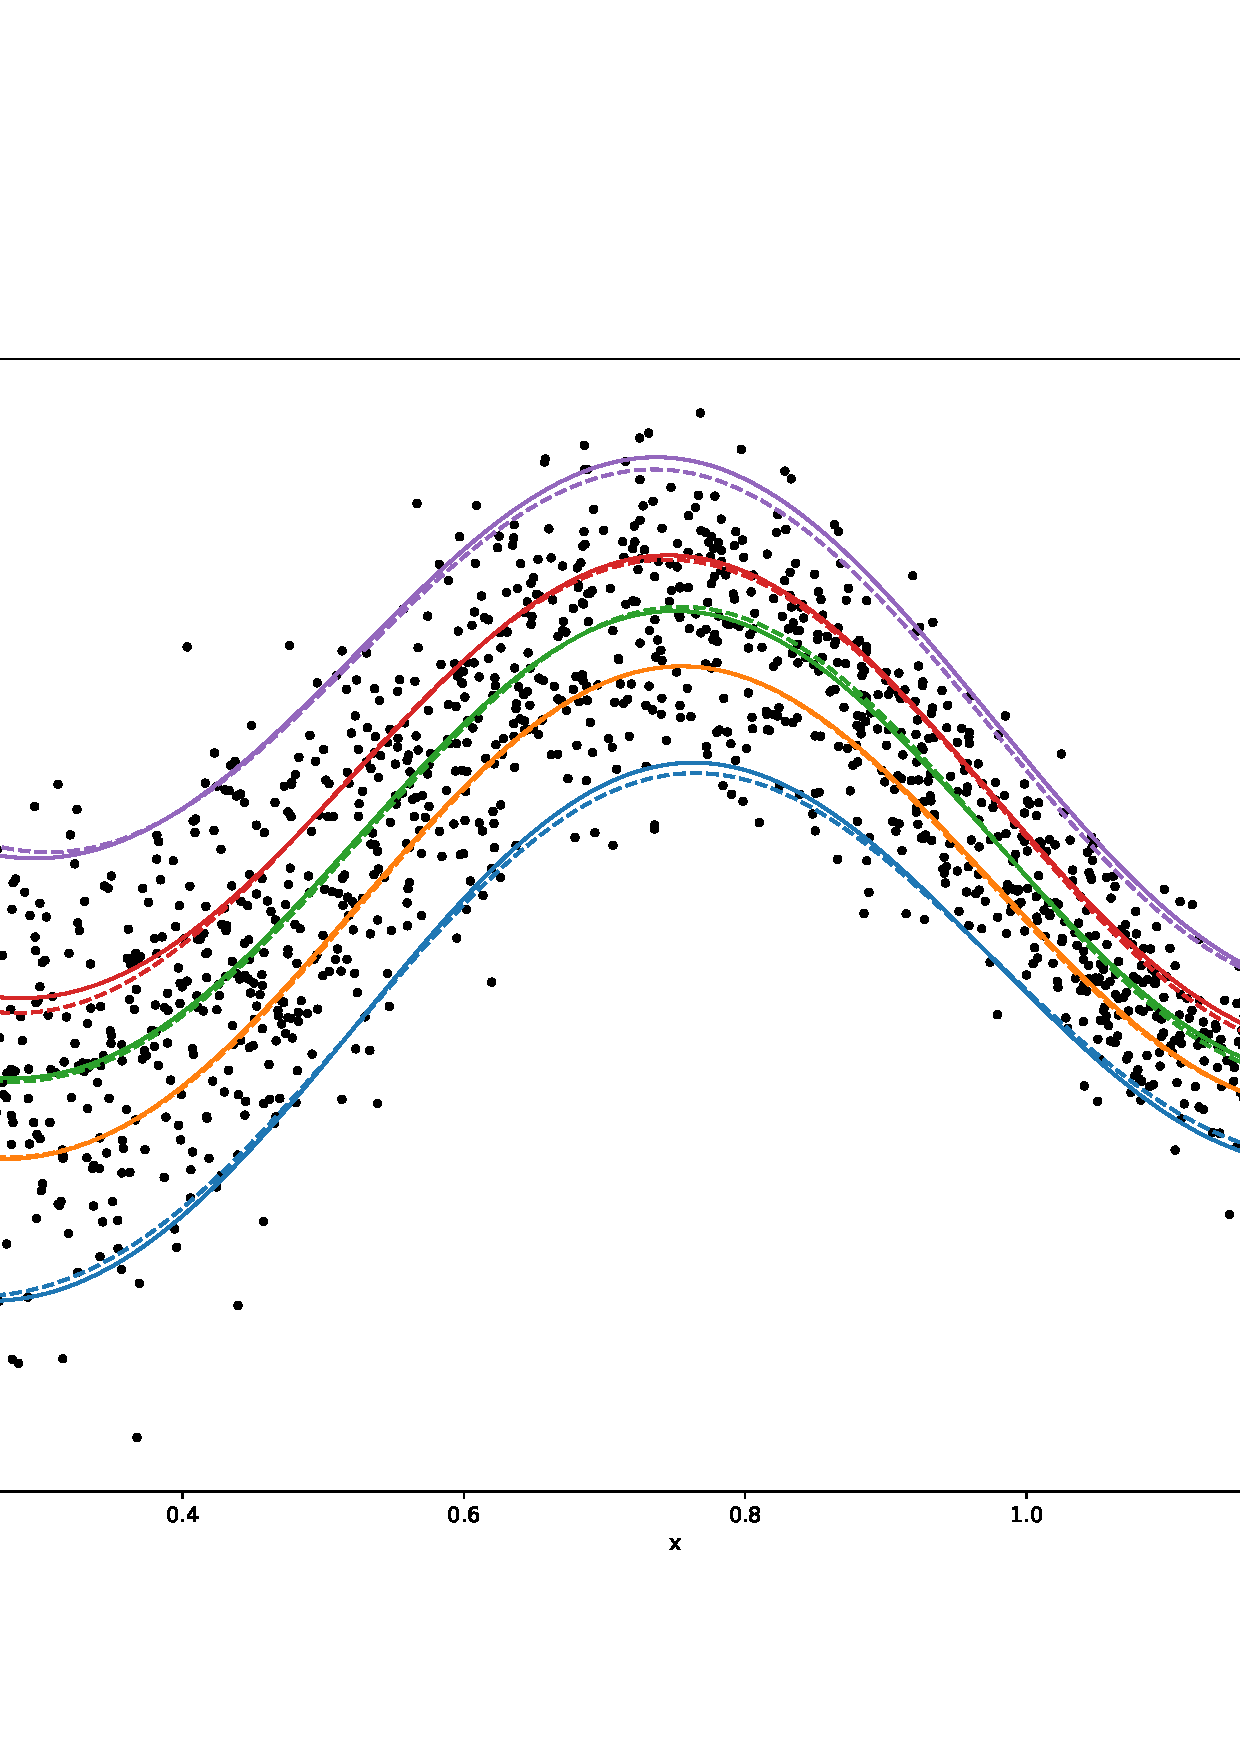
\includegraphics{./gfx/quantile_orff.pdf}}
        \caption{Learning a continuous quantile function with ORFF
        regression. \label{fig:quantile_orff}}
    \end{figure}
    \clearpage
    \begin{figure}[htp]
        \centering\resizebox{.8\textheight}{!}{%
        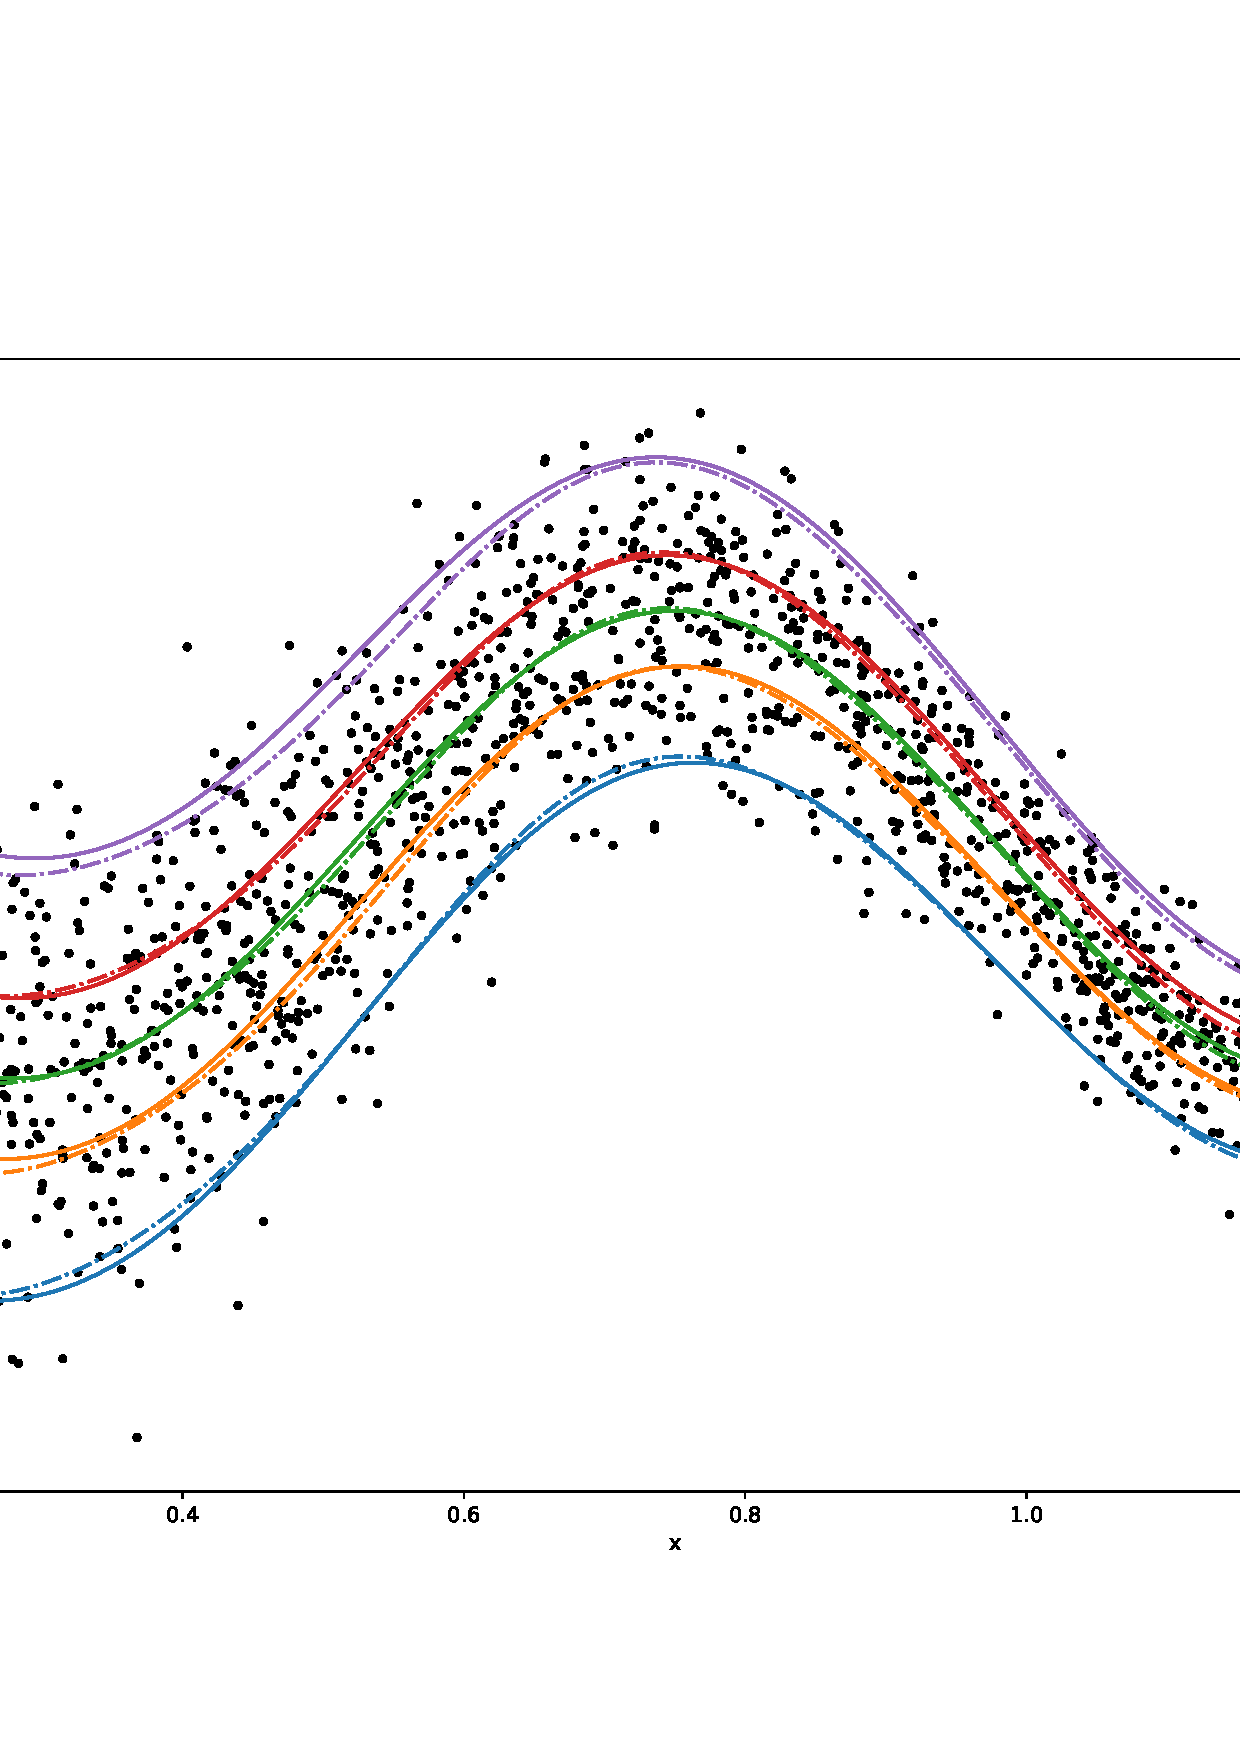
\includegraphics{./gfx/quantile_joint.pdf}}
        \caption{Learning many quantile with joint OVK regression.
        \label{fig:quantile_joint}}
    \end{figure}
\end{landscape}}
Moreover $W^\adjoint W$ is the identity on
$\Ima \Phi_{\tau}$ which is here $\mathcal{H}_{k_{\mathcal{T}}}$. (see the
proof of \cref{pr:feature_operator} and \citet{Carmeli2010}). Thus we can
choose $\Phi_\tau=\Phi(\tau)$ to be the functional Fourier feature map
associated to $k_{\mathcal{T}}$ defined in \cref{pr:fourier_feature_map}.  Then
we have $BB^\adjoint = I_{\mathcal{H}_{k_{\mathcal{T}}}} = W^\adjoint W$.  Thus
we can choose $B^\adjoint = W = \Phi(\cdot)^\adjoint$ and the approximate
feature map reads 
\begin{dmath*}
    \tildePhi{\omega}(x)\in \mathcal{L}\left(\mathcal{H}_{k_{\mathcal{T}}};
    \Vect_{j=1}^D L^2\left(\dual{\mathcal{T}},
    \probability_{\dual{\Haar},\rho}\right)\right)
\end{dmath*}
and
\begin{dmath*}
    (\tildePhi{\omega}(x)g)(\tau) = \frac{1}{\sqrt{D}}\Vect_{j=1}^D
    \begin{pmatrix}
        \cos(x \omega_j) \Phi(\tau)^\adjoint g \\
        \sin(x \omega_j) \Phi(\tau)^\adjoint g
    \end{pmatrix} \condition{$\omega_j \sim \FT{k_{\mathcal{X}}}$
    \ac{iid}}
\end{dmath*}
Then as proposed in \cref{ch:operator-valued_random_fourier_features} we can
Monte-Carlo sample the functional feature map $\Phi(\tau)$ and obtain the 
\acs{ORFF} map 
\begin{dmath*}
    \left(\widetilde{\tildePhi{\omega}}(x)g\right)(\tau) =
    \frac{1}{\sqrt{DD'}}\Vect_{j=1}^D
    \begin{pmatrix}
        \cos(x \omega_j) \sum_{k=1}^{D'}
        \left(\cos(\tau \omega_k') + \sin(\tau \omega_k')\right)g(\omega_k') \\
        \sin(x \omega_j) \sum_{k=1}^{D'}
        \left(\cos(\tau \omega_k') + \sin(\tau \omega_k')\right)g(\omega_k')
    \end{pmatrix} \condition{$\omega_j \sim \FT{k_{\mathcal{X}}}$
    \acs{iid} and $\omega_k'\sim \FT{k_{\mathcal{T}}}$ \acs{iid}.}
\end{dmath*}
where $g\in L^2\left(\dual{\mathcal{T}}, \probability_{\dual{\Haar},
\rho}\right)$ and $\tau\in\mathbb{R}$. If we note 
\begin{dmath*}
    G = 
    \begin{pmatrix}
        g(\omega_1') & \dots & g(\omega_{D'}') 
    \end{pmatrix}^\adjoint \hiderel{\in} \mathbb{R}^{D'}
\end{dmath*}
we can define
\begin{dmath*}
    \left(\widetilde{\tildePhi{\omega}}(x)G\right)(\tau) =
    \frac{1}{\sqrt{DD'}}\Vect_{j=1}^D
    \begin{pmatrix}
        \cos(x \omega_j) \sum_{k=1}^{D'}
        \left(\cos(\tau \omega_k') + \sin(\tau \omega_k')\right)G_k \\
        \sin(x \omega_j) \sum_{k=1}^{D'}
        \left(\cos(\tau \omega_k') + \sin(\tau \omega_k')\right)G_k
    \end{pmatrix} \condition{$\omega_j \sim \FT{k_{\mathcal{X}}}$
    \acs{iid} and $\omega_k'\sim \FT{k_{\mathcal{T}}}$ \acs{iid}.}
\end{dmath*}
Then it is easy to verify that the adjoint operator is given by
\begin{dmath*}
    \left(\widetilde{\tildePhi{\omega}}(x)^\adjoint \theta\right)(\tau) =
    \frac{1}{\sqrt{DD'}} \sum_{j=1}^D \left(\cos(x\omega_j) +
    \sin(x\omega_j)\right) \left(\Vect_{k=1}^{D'}
    \begin{pmatrix}
        \cos(\tau \omega_k') \\
        \sin(\tau \omega_k')
    \end{pmatrix}\right)^\adjoint \theta_j
    = \frac{1}{\sqrt{DD'}} \sum_{j=1}^D \left(\cos(x\omega_j) +
    \sin(x\omega_j)\right) \theta_{jk} \left( \cos(\tau \omega_k') + \sin(\tau
    \omega_k')\right)
    \condition{$\omega_j \sim \FT{k_{\mathcal{X}}}$
    \acs{iid} and $\omega_k'\sim \FT{k_{\mathcal{T}}}$ \acs{iid}.}
\end{dmath*}
where $\theta_k\in\mathbb{R}^{D'}$, for all $k \in \mathbb{N}^*_D$ and
$\theta_{jk}\in\mathbb{R}$ for all $j \in \mathbb{N}^*_D$ and all $k \in
\mathbb{N}^*_{D'}$. The above equations can be rewritten in matrix form which
results in the following conjecture.
\begin{conjecture}
    \label{cj:functional_orff}
    If $\tildephi{\omega}_{\mathcal{X}}$ is an \acs{RFF} for
    $\widetilde{k}_{\mathcal{X}}$ such that
    $\tildephi{\omega}(x)\in\mathbb{R}^D$ and $\tildephi{\omega}_{\mathcal{T}}$
    is an \acs{RFF} for $\widetilde{k}_{\mathcal{T}}$, such that
    $\tildephi{\omega}(\tau)\in\mathbb{R}^{D'}$ then an \acs{ORFF} map for
    \begin{dmath*}
        K(x, z) = k_{\mathcal{X}}(x, z) I_{\mathcal{H}_{k_{\mathcal{T}}}}
    \end{dmath*}
    is given for all $x\in\mathbb{R}$, all $\tau\in\mathbb{R}$ and all
    $\Theta\in\mathcal{M}_{D,D'}(\mathbb{R})$ by
    \begin{dmath*}
        \left(\tildePhi{\omega}_K(x)^\adjoint \Theta \right)(\tau) =
        \tildephi{\omega}_{\mathcal{X}}(x)^\adjoint \Theta
        \tildephi{\omega}_{\mathcal{T}}(\tau)
    \end{dmath*}
    and
    \begin{dmath*}
        \left(\tildePhi{\omega}_K(x) G\right)(\tau) =
        \tildephi{\omega}_{\mathcal{X}}(x)
        \tildephi{\omega}_{\mathcal{T}}(\tau)^\adjoint G,
    \end{dmath*}
    where $g\in\mathbb{R}^{D'}$.
    %but more intestingly, given $y\in\mathbb{R}$,
    %\begin{dmath*}
        %\tildePhi{\omega}_K(x, \tau)^\adjoint y =
        %y \tildephi{\omega}_{\mathcal{X}}(x)
        %\tildephi{\omega}_{\mathcal{T}}(\tau)^\adjoint.
    %\end{dmath*}
\end{conjecture}
Moreover if one defines $\tildePhi{\omega}_K(x,
\tau) = \left(\tildePhi{\omega}_K(x)^\adjoint \Theta \right)(\tau)$ one
have of course
\begin{dmath*}
    \tildePhi{\omega}_K(x, \tau)^\adjoint \Theta =
    \tildephi{\omega}_{\mathcal{X}}(x)^\adjoint \Theta
    \tildephi{\omega}_{\mathcal{T}}(\tau)
\end{dmath*}
\subsection{Many quantile regression}
From the loss defined in \cref{eq:loss_pinball} we defined the regularized risk
using the \say{continuous} pinball loss for the quantile regression problem.
For all $f\in\mathcal{H}_K$,
\begin{dmath*}
    J_{\lambda}(f) =
    \frac{1}{N}\sum_{i=1}^N\int_{[0,1]}\left(
    \begin{cases}
        \tau\left(f_{x_i}(\tau) - y_i\right) & \text{if } f_{x_i}(\tau) \ge y_i
        \\
        (1 - \tau)\left(y_i - f_{x_i}(\tau)\right) & \text{otherwise} 
    \end{cases} \right)+ \lambda
    \norm{f}_K^2.
\end{dmath*}
The issue with the above risk is that the different quantile for a given point
$x\in\mathbb{R}$ may cross \citet{sangnier2016joint}. To avoid this to happen
we need to force the function $f_x(\tau)$ to be \emph{increasing} in $\tau$ for
any $x\in\mathbb{R}$.  Because a decreasing function has a negative derivative
we can add a penalty term to the risk to avoid $f_x(\tau)$ to be decreasing in
$\tau$.
\begin{dmath*}
    \Omega_{cross}(f) = - \min\left(\frac{\partial
    f_{x_i}}{\partial\tau}(\tau),
    0\right)
\end{dmath*}
Thus the regularized risk with the no crossing constraint is
\begin{dmath*}
    J_{\lambda_1, \lambda_2}(f) =
    \frac{1}{N}\sum_{i=1}^N\int_{[0,1]}\left(
    \begin{cases} 
        \tau \left(f_{x_i}(\tau) - y_i\right) & \text{if } f_{x_i}(\tau) \ge
        y_i \\
        (1 - \tau)\left(y_i - f_{x_i}(\tau)\right) & \text{otherwise}
    \end{cases} -
    \lambda_1 \min\left(\frac{\partial f_{x_i}}{\partial\tau}(\tau), 0\right)
    \right)+ \lambda_2 \norm{f}_K^2.
\end{dmath*}
Eventually we replace the integral by a Monte-Carlo sampling with the uniform
law $\mathcal{U}([0, 1])$ and plug in the approximate function of $f$ using the
\acs{ORFF} map proposed in \cref{cj:functional_orff}. The final optimzation
problem reads
\begin{dmath*}
    J_{\lambda_1, \lambda_2}(\Theta) =
    \frac{1}{NT}\sum_{i=1}^N\sum_{t=1}^T\left(
    \begin{cases} \tau_t
        \left(\widetilde{f}_{x_i}(\tau_t) - y_i\right) & \text{if }
        \widetilde{f}_{x_i}(\tau_t) \ge y_i \\
        (1 - \tau_t)\left(y_i - f_{x_i}(\tau_t)\right) & \text{otherwise} 
    \end{cases} - \lambda_1
    \min\left(\frac{\partial \widetilde{f}_{x_i}}{\partial\tau}(\tau_t),
    0\right) \right)+ \lambda_2 \norm{\Theta}_{fro}^2.
\end{dmath*}
where $\widetilde{f}_{x}(\tau)=\tildephi{\omega}_{\mathcal{X}}(x)^\adjoint
\Theta \tildephi{\omega}_{\mathcal{T}}(\tau)$, $\tau_t \sim \mathcal{U}([0,
1])$ and
\begin{dmath*}
    \frac{\partial \widetilde{f}_{x}}{\partial\tau}(\tau)
    = \tildephi{\omega}_{\mathcal{X}}(x)^\adjoint \Theta \frac{\partial
    \tildephi{\omega}_{\mathcal{T}}}{\partial \tau}(\tau)
    = \tildephi{\omega}_{\mathcal{X}}(x)^\adjoint \Theta \Vect_{k=1}^{D'}
    \begin{pmatrix}
        -\omega_k' \sin(\omega_k' x) \\
         \omega_k' \cos(\omega_k' x)
    \end{pmatrix} \condition{$\omega_k' \sim \FT{k_{\mathcal{T}}}$ \acs{iid}.}
\end{dmath*}
\subsubsection{Some results}
We minimize the quantity $J_{\lambda_1, \lambda_2}(\Theta)$ on a toy dataset: a
sine wave with some heteroskedastic noise. First we compare our methodology to
the joint quantile regression proposed in \citet{sangnier2016joint}. We
generate $N=2500$ for the train set and $N'=1000$ points for the test set and
use a gaussian kernel for both $k_{\mathcal{X}}$ and $k_{\mathcal{T}}$. We
choosed $\sigma_{\mathcal{X}} = 0.25$ and $\sigma_{\mathcal{T}}$ is set to be
the median of the pairwise distance of the $\tau_t$'s drawn randomly from
$\mathcal{U}([0, 1])$. Notice that $J_{\lambda_1, \lambda_2}(\Theta)$ is convex
in $\Theta$. To avoid computing complex gradients and by lack of time, we used
Tensorflow \citep{abadi2016tensorflow} to perform a gradient descent (with
RMSProp \citep{tieleman2012lecture}) with automatic symbolic differentiation.
\Cref{fig:quantile_orff} show the result for the quantile at $0.05$, $0.275$,
$0.5$, $0.775$ and $0.95$ using the \acs{ORFF} methodology. 
\afterpage{%
\begin{landscape}
    \begin{figure}[htp]
        \centering
        \resizebox{.8\textheight}{!}{%
        \includegraphics{./gfx/quantile_continuous.pgf}}
        \caption{Learning a continuous quantile function with ORFF
        regression. \label{fig:quantile_continuous}}
    \end{figure}
\end{landscape}}
\Cref{fig:quantile_joint} shows the joint quantile regression of
\citet{sangnier2016joint} on the same dataset. Not only our method matches the
the performances of \citet{sangnier2016joint}\footnote{We reported an error
computed with the pinball loss on the test set of $0.818$ for our method and
$0.817$ for joint regression (note that we don't report here an average on many
experiments to avoid randomness introduced by the random features, but the
results seems robust in practice.)} but we cut down the computation time from
circa $1330$ seconds to circa $30$ seconds (training and testing).  Moreover on
contrary to \citet{sangnier2016joint} we have access to all the quantile of the
model (see \cref{fig:quantile_continuous}).

\subsection{One-class SVM revisited}
We also propose an extension of the celebrated \acf{OCSVM} so that it
possible to learn jointly all the level sets.  One-class classification, also
known as unary classification, tries to identify objects of a specific class
amongst all objects, by learning from a training set containing only the
objects of that class.  In this framework, we assume that we only observe
examples of one class (referred to as the inlier class).  The second class is
called outlier class.  We turn our attention to the \acs{OCSVM}
of \citet{Scholkopf2001} which extends the \ac{SVM} methodology
\citep{Cortes1995,Shawe2004} to handle training using only inliers. 
\paragraph{}
We recall that given an hyperparameter $\nu\in [0,1]$ that controls the
proportion of inlier, given as scalar kernel $k$, the \acs{OCSVM} problem reads
\begin{dmath*}
    \argmin_{f\in\mathcal{H}_k, \tau \in \mathbb{R}} \frac{1}{2}
    \norm{f}_{\mathcal{H}_k}^2 - \nu \tau + \frac{1}{N} \sum_{i=1}^N \max(\tau
    - f(x_i), 0)
\end{dmath*}
The decision function is then
\begin{dmath*}
    h(x, \tau) = \mathds{1}_{[\tau, \infty)}\left( f(x) \right).
\end{dmath*}
As in \cref{subsec:quantile_regression} we can rewrite the optimization problem
as an integral over all the value of $\nu$ and suppose that $f$ is
function-valued (a function of $\nu$). Moreover $\tau$ must also change its
value according to $\mu$. Thus given a kernel $k_{\mathcal{X}}$ on the inputs
$x\in\mathbb{R}^d$ with its approximate feature map
$\tildephi{\omega}_{\mathcal{X}}$ and a kernel $k_{\mathcal{T}}$ on the level
sets with its approximate feature map $\tildephi{\omega}_{\mathcal{T}}$, we
define the continuous one-class SVM problem as
\begin{dmath*}
    \argmin_{f
    \in\mathcal{H}_K,\tau\in\mathcal{H}_{k_{\mathcal{\tau}}}}\frac{1}{N}
    \sum_{i=1}^N\int_{[0,1]}\max\left(0, \tau(\nu) - f_{x_i}(\nu)\right)d\nu +
    \frac{1}{2}\int_{[0,1]}\nu
    \norm{f_{\cdot}(\nu)}_{\mathcal{H}_{k_{\mathcal{X}}}}^2d\nu -
    \int_{[0,1]}\nu\tau(\nu)d\nu.
\end{dmath*}
Again we can compute the integral by Monte-Carlo sampling and replace $f$ and
$\tau$ by their respective approximation. Notice that the \acs{RKHS} of $\tau$
should match the \acs{RKHS} of the output space of $f_K$. Hence
\begin{dmath*}
    \argmin_{\Theta
    \in\mathcal{M}_{D, D'}(\mathbb{R}),\tau\in\mathbb{R}^D}\frac{1}{NT}
    \sum_{i=1}^N\sum_{t=1}^T\max\left(0, \widetilde{\tau}(\nu_t) -
    \widetilde{f}_{x_i}(\nu_t)\right) + \frac{1}{2T}\sum_{t=1}^T\nu_t
    \norm{\widetilde{f}_{\cdot}(\nu_t)}_{2}^2 -
    \frac{1}{T}\sum_{t=1}^T\nu_t\widetilde{\tau}(\nu_t),
\end{dmath*}
where $\nu_t \sim \mathcal{U}([0, 1])$ \acs{iid}, $\widetilde{\tau}(\nu) =
\tildephi{\omega}_{\mathcal{T}}(\nu)$ and $\widetilde{f}_x(\nu) =
\tildephi{\omega}(x)^\adjoint \Theta \tildephi{\omega}_{\mathcal{T}}(\nu)$. We
also deduce that $\widetilde{f}_{\cdot}(\nu) = \Theta
\tildephi{\omega}_{\mathcal{T}}(\nu)$. Here the natural decision function is
\begin{dmath}
    \label{eq:continuous_decision}
    h(x, \nu) = \mathds{1}_{\left[\widetilde{\tau}(\nu),\infty\right)}
    \left(\widetilde{f}_x(\nu)\right).
\end{dmath}
\begin{figure}
    {\centering
    \resizebox{2\textwidth}{!}{%% Creator: Matplotlib, PGF backend
%%
%% To include the figure in your LaTeX document, write
%%   \input{<filename>.pgf}
%%
%% Make sure the required packages are loaded in your preamble
%%   \usepackage{pgf}
%%
%% Figures using additional raster images can only be included by \input if
%% they are in the same directory as the main LaTeX file. For loading figures
%% from other directories you can use the `import` package
%%   \usepackage{import}
%% and then include the figures with
%%   \import{<path to file>}{<filename>.pgf}
%%
%% Matplotlib used the following preamble
%%   \usepackage{fontspec}
%%   \setmainfont{Times New Roman}
%%   \setsansfont{Lucida Grande}
%%   \setmonofont{Andale Mono}
%%
\begingroup%
\makeatletter%
\begin{pgfpicture}%
\pgfpathrectangle{\pgfpointorigin}{\pgfqpoint{16.000000in}{5.000000in}}%
\pgfusepath{use as bounding box, clip}%
\begin{pgfscope}%
\pgfsetbuttcap%
\pgfsetmiterjoin%
\definecolor{currentfill}{rgb}{1.000000,1.000000,1.000000}%
\pgfsetfillcolor{currentfill}%
\pgfsetlinewidth{0.000000pt}%
\definecolor{currentstroke}{rgb}{1.000000,1.000000,1.000000}%
\pgfsetstrokecolor{currentstroke}%
\pgfsetdash{}{0pt}%
\pgfpathmoveto{\pgfqpoint{0.000000in}{0.000000in}}%
\pgfpathlineto{\pgfqpoint{16.000000in}{0.000000in}}%
\pgfpathlineto{\pgfqpoint{16.000000in}{5.000000in}}%
\pgfpathlineto{\pgfqpoint{0.000000in}{5.000000in}}%
\pgfpathclose%
\pgfusepath{fill}%
\end{pgfscope}%
\begin{pgfscope}%
\pgfsetbuttcap%
\pgfsetmiterjoin%
\definecolor{currentfill}{rgb}{1.000000,1.000000,1.000000}%
\pgfsetfillcolor{currentfill}%
\pgfsetlinewidth{0.000000pt}%
\definecolor{currentstroke}{rgb}{0.000000,0.000000,0.000000}%
\pgfsetstrokecolor{currentstroke}%
\pgfsetstrokeopacity{0.000000}%
\pgfsetdash{}{0pt}%
\pgfpathmoveto{\pgfqpoint{0.663889in}{0.580556in}}%
\pgfpathlineto{\pgfqpoint{8.157639in}{0.580556in}}%
\pgfpathlineto{\pgfqpoint{8.157639in}{4.801389in}}%
\pgfpathlineto{\pgfqpoint{0.663889in}{4.801389in}}%
\pgfpathclose%
\pgfusepath{fill}%
\end{pgfscope}%
\begin{pgfscope}%
\pgfsetbuttcap%
\pgfsetroundjoin%
\definecolor{currentfill}{rgb}{0.000000,0.000000,0.000000}%
\pgfsetfillcolor{currentfill}%
\pgfsetlinewidth{0.803000pt}%
\definecolor{currentstroke}{rgb}{0.000000,0.000000,0.000000}%
\pgfsetstrokecolor{currentstroke}%
\pgfsetdash{}{0pt}%
\pgfsys@defobject{currentmarker}{\pgfqpoint{0.000000in}{-0.048611in}}{\pgfqpoint{0.000000in}{0.000000in}}{%
\pgfpathmoveto{\pgfqpoint{0.000000in}{0.000000in}}%
\pgfpathlineto{\pgfqpoint{0.000000in}{-0.048611in}}%
\pgfusepath{stroke,fill}%
}%
\begin{pgfscope}%
\pgfsys@transformshift{1.004514in}{0.580556in}%
\pgfsys@useobject{currentmarker}{}%
\end{pgfscope}%
\end{pgfscope}%
\begin{pgfscope}%
\pgftext[x=1.004514in,y=0.483333in,,top]{\sffamily\fontsize{10.000000}{12.000000}\selectfont 0.0}%
\end{pgfscope}%
\begin{pgfscope}%
\pgfsetbuttcap%
\pgfsetroundjoin%
\definecolor{currentfill}{rgb}{0.000000,0.000000,0.000000}%
\pgfsetfillcolor{currentfill}%
\pgfsetlinewidth{0.803000pt}%
\definecolor{currentstroke}{rgb}{0.000000,0.000000,0.000000}%
\pgfsetstrokecolor{currentstroke}%
\pgfsetdash{}{0pt}%
\pgfsys@defobject{currentmarker}{\pgfqpoint{0.000000in}{-0.048611in}}{\pgfqpoint{0.000000in}{0.000000in}}{%
\pgfpathmoveto{\pgfqpoint{0.000000in}{0.000000in}}%
\pgfpathlineto{\pgfqpoint{0.000000in}{-0.048611in}}%
\pgfusepath{stroke,fill}%
}%
\begin{pgfscope}%
\pgfsys@transformshift{2.367014in}{0.580556in}%
\pgfsys@useobject{currentmarker}{}%
\end{pgfscope}%
\end{pgfscope}%
\begin{pgfscope}%
\pgftext[x=2.367014in,y=0.483333in,,top]{\sffamily\fontsize{10.000000}{12.000000}\selectfont 0.2}%
\end{pgfscope}%
\begin{pgfscope}%
\pgfsetbuttcap%
\pgfsetroundjoin%
\definecolor{currentfill}{rgb}{0.000000,0.000000,0.000000}%
\pgfsetfillcolor{currentfill}%
\pgfsetlinewidth{0.803000pt}%
\definecolor{currentstroke}{rgb}{0.000000,0.000000,0.000000}%
\pgfsetstrokecolor{currentstroke}%
\pgfsetdash{}{0pt}%
\pgfsys@defobject{currentmarker}{\pgfqpoint{0.000000in}{-0.048611in}}{\pgfqpoint{0.000000in}{0.000000in}}{%
\pgfpathmoveto{\pgfqpoint{0.000000in}{0.000000in}}%
\pgfpathlineto{\pgfqpoint{0.000000in}{-0.048611in}}%
\pgfusepath{stroke,fill}%
}%
\begin{pgfscope}%
\pgfsys@transformshift{3.729514in}{0.580556in}%
\pgfsys@useobject{currentmarker}{}%
\end{pgfscope}%
\end{pgfscope}%
\begin{pgfscope}%
\pgftext[x=3.729514in,y=0.483333in,,top]{\sffamily\fontsize{10.000000}{12.000000}\selectfont 0.4}%
\end{pgfscope}%
\begin{pgfscope}%
\pgfsetbuttcap%
\pgfsetroundjoin%
\definecolor{currentfill}{rgb}{0.000000,0.000000,0.000000}%
\pgfsetfillcolor{currentfill}%
\pgfsetlinewidth{0.803000pt}%
\definecolor{currentstroke}{rgb}{0.000000,0.000000,0.000000}%
\pgfsetstrokecolor{currentstroke}%
\pgfsetdash{}{0pt}%
\pgfsys@defobject{currentmarker}{\pgfqpoint{0.000000in}{-0.048611in}}{\pgfqpoint{0.000000in}{0.000000in}}{%
\pgfpathmoveto{\pgfqpoint{0.000000in}{0.000000in}}%
\pgfpathlineto{\pgfqpoint{0.000000in}{-0.048611in}}%
\pgfusepath{stroke,fill}%
}%
\begin{pgfscope}%
\pgfsys@transformshift{5.092014in}{0.580556in}%
\pgfsys@useobject{currentmarker}{}%
\end{pgfscope}%
\end{pgfscope}%
\begin{pgfscope}%
\pgftext[x=5.092014in,y=0.483333in,,top]{\sffamily\fontsize{10.000000}{12.000000}\selectfont 0.6}%
\end{pgfscope}%
\begin{pgfscope}%
\pgfsetbuttcap%
\pgfsetroundjoin%
\definecolor{currentfill}{rgb}{0.000000,0.000000,0.000000}%
\pgfsetfillcolor{currentfill}%
\pgfsetlinewidth{0.803000pt}%
\definecolor{currentstroke}{rgb}{0.000000,0.000000,0.000000}%
\pgfsetstrokecolor{currentstroke}%
\pgfsetdash{}{0pt}%
\pgfsys@defobject{currentmarker}{\pgfqpoint{0.000000in}{-0.048611in}}{\pgfqpoint{0.000000in}{0.000000in}}{%
\pgfpathmoveto{\pgfqpoint{0.000000in}{0.000000in}}%
\pgfpathlineto{\pgfqpoint{0.000000in}{-0.048611in}}%
\pgfusepath{stroke,fill}%
}%
\begin{pgfscope}%
\pgfsys@transformshift{6.454514in}{0.580556in}%
\pgfsys@useobject{currentmarker}{}%
\end{pgfscope}%
\end{pgfscope}%
\begin{pgfscope}%
\pgftext[x=6.454514in,y=0.483333in,,top]{\sffamily\fontsize{10.000000}{12.000000}\selectfont 0.8}%
\end{pgfscope}%
\begin{pgfscope}%
\pgfsetbuttcap%
\pgfsetroundjoin%
\definecolor{currentfill}{rgb}{0.000000,0.000000,0.000000}%
\pgfsetfillcolor{currentfill}%
\pgfsetlinewidth{0.803000pt}%
\definecolor{currentstroke}{rgb}{0.000000,0.000000,0.000000}%
\pgfsetstrokecolor{currentstroke}%
\pgfsetdash{}{0pt}%
\pgfsys@defobject{currentmarker}{\pgfqpoint{0.000000in}{-0.048611in}}{\pgfqpoint{0.000000in}{0.000000in}}{%
\pgfpathmoveto{\pgfqpoint{0.000000in}{0.000000in}}%
\pgfpathlineto{\pgfqpoint{0.000000in}{-0.048611in}}%
\pgfusepath{stroke,fill}%
}%
\begin{pgfscope}%
\pgfsys@transformshift{7.817014in}{0.580556in}%
\pgfsys@useobject{currentmarker}{}%
\end{pgfscope}%
\end{pgfscope}%
\begin{pgfscope}%
\pgftext[x=7.817014in,y=0.483333in,,top]{\sffamily\fontsize{10.000000}{12.000000}\selectfont 1.0}%
\end{pgfscope}%
\begin{pgfscope}%
\pgftext[x=4.410764in,y=0.293908in,,top]{\sffamily\fontsize{10.000000}{12.000000}\selectfont \(\displaystyle \nu\)}%
\end{pgfscope}%
\begin{pgfscope}%
\pgfsetbuttcap%
\pgfsetroundjoin%
\definecolor{currentfill}{rgb}{0.000000,0.000000,0.000000}%
\pgfsetfillcolor{currentfill}%
\pgfsetlinewidth{0.803000pt}%
\definecolor{currentstroke}{rgb}{0.000000,0.000000,0.000000}%
\pgfsetstrokecolor{currentstroke}%
\pgfsetdash{}{0pt}%
\pgfsys@defobject{currentmarker}{\pgfqpoint{-0.048611in}{0.000000in}}{\pgfqpoint{0.000000in}{0.000000in}}{%
\pgfpathmoveto{\pgfqpoint{0.000000in}{0.000000in}}%
\pgfpathlineto{\pgfqpoint{-0.048611in}{0.000000in}}%
\pgfusepath{stroke,fill}%
}%
\begin{pgfscope}%
\pgfsys@transformshift{0.663889in}{0.772412in}%
\pgfsys@useobject{currentmarker}{}%
\end{pgfscope}%
\end{pgfscope}%
\begin{pgfscope}%
\pgftext[x=0.347076in,y=0.718870in,left,base]{\sffamily\fontsize{10.000000}{12.000000}\selectfont 0.0}%
\end{pgfscope}%
\begin{pgfscope}%
\pgfsetbuttcap%
\pgfsetroundjoin%
\definecolor{currentfill}{rgb}{0.000000,0.000000,0.000000}%
\pgfsetfillcolor{currentfill}%
\pgfsetlinewidth{0.803000pt}%
\definecolor{currentstroke}{rgb}{0.000000,0.000000,0.000000}%
\pgfsetstrokecolor{currentstroke}%
\pgfsetdash{}{0pt}%
\pgfsys@defobject{currentmarker}{\pgfqpoint{-0.048611in}{0.000000in}}{\pgfqpoint{0.000000in}{0.000000in}}{%
\pgfpathmoveto{\pgfqpoint{0.000000in}{0.000000in}}%
\pgfpathlineto{\pgfqpoint{-0.048611in}{0.000000in}}%
\pgfusepath{stroke,fill}%
}%
\begin{pgfscope}%
\pgfsys@transformshift{0.663889in}{1.539836in}%
\pgfsys@useobject{currentmarker}{}%
\end{pgfscope}%
\end{pgfscope}%
\begin{pgfscope}%
\pgftext[x=0.347076in,y=1.486294in,left,base]{\sffamily\fontsize{10.000000}{12.000000}\selectfont 0.2}%
\end{pgfscope}%
\begin{pgfscope}%
\pgfsetbuttcap%
\pgfsetroundjoin%
\definecolor{currentfill}{rgb}{0.000000,0.000000,0.000000}%
\pgfsetfillcolor{currentfill}%
\pgfsetlinewidth{0.803000pt}%
\definecolor{currentstroke}{rgb}{0.000000,0.000000,0.000000}%
\pgfsetstrokecolor{currentstroke}%
\pgfsetdash{}{0pt}%
\pgfsys@defobject{currentmarker}{\pgfqpoint{-0.048611in}{0.000000in}}{\pgfqpoint{0.000000in}{0.000000in}}{%
\pgfpathmoveto{\pgfqpoint{0.000000in}{0.000000in}}%
\pgfpathlineto{\pgfqpoint{-0.048611in}{0.000000in}}%
\pgfusepath{stroke,fill}%
}%
\begin{pgfscope}%
\pgfsys@transformshift{0.663889in}{2.307260in}%
\pgfsys@useobject{currentmarker}{}%
\end{pgfscope}%
\end{pgfscope}%
\begin{pgfscope}%
\pgftext[x=0.347076in,y=2.253719in,left,base]{\sffamily\fontsize{10.000000}{12.000000}\selectfont 0.4}%
\end{pgfscope}%
\begin{pgfscope}%
\pgfsetbuttcap%
\pgfsetroundjoin%
\definecolor{currentfill}{rgb}{0.000000,0.000000,0.000000}%
\pgfsetfillcolor{currentfill}%
\pgfsetlinewidth{0.803000pt}%
\definecolor{currentstroke}{rgb}{0.000000,0.000000,0.000000}%
\pgfsetstrokecolor{currentstroke}%
\pgfsetdash{}{0pt}%
\pgfsys@defobject{currentmarker}{\pgfqpoint{-0.048611in}{0.000000in}}{\pgfqpoint{0.000000in}{0.000000in}}{%
\pgfpathmoveto{\pgfqpoint{0.000000in}{0.000000in}}%
\pgfpathlineto{\pgfqpoint{-0.048611in}{0.000000in}}%
\pgfusepath{stroke,fill}%
}%
\begin{pgfscope}%
\pgfsys@transformshift{0.663889in}{3.074684in}%
\pgfsys@useobject{currentmarker}{}%
\end{pgfscope}%
\end{pgfscope}%
\begin{pgfscope}%
\pgftext[x=0.347076in,y=3.021143in,left,base]{\sffamily\fontsize{10.000000}{12.000000}\selectfont 0.6}%
\end{pgfscope}%
\begin{pgfscope}%
\pgfsetbuttcap%
\pgfsetroundjoin%
\definecolor{currentfill}{rgb}{0.000000,0.000000,0.000000}%
\pgfsetfillcolor{currentfill}%
\pgfsetlinewidth{0.803000pt}%
\definecolor{currentstroke}{rgb}{0.000000,0.000000,0.000000}%
\pgfsetstrokecolor{currentstroke}%
\pgfsetdash{}{0pt}%
\pgfsys@defobject{currentmarker}{\pgfqpoint{-0.048611in}{0.000000in}}{\pgfqpoint{0.000000in}{0.000000in}}{%
\pgfpathmoveto{\pgfqpoint{0.000000in}{0.000000in}}%
\pgfpathlineto{\pgfqpoint{-0.048611in}{0.000000in}}%
\pgfusepath{stroke,fill}%
}%
\begin{pgfscope}%
\pgfsys@transformshift{0.663889in}{3.842109in}%
\pgfsys@useobject{currentmarker}{}%
\end{pgfscope}%
\end{pgfscope}%
\begin{pgfscope}%
\pgftext[x=0.347076in,y=3.788567in,left,base]{\sffamily\fontsize{10.000000}{12.000000}\selectfont 0.8}%
\end{pgfscope}%
\begin{pgfscope}%
\pgfsetbuttcap%
\pgfsetroundjoin%
\definecolor{currentfill}{rgb}{0.000000,0.000000,0.000000}%
\pgfsetfillcolor{currentfill}%
\pgfsetlinewidth{0.803000pt}%
\definecolor{currentstroke}{rgb}{0.000000,0.000000,0.000000}%
\pgfsetstrokecolor{currentstroke}%
\pgfsetdash{}{0pt}%
\pgfsys@defobject{currentmarker}{\pgfqpoint{-0.048611in}{0.000000in}}{\pgfqpoint{0.000000in}{0.000000in}}{%
\pgfpathmoveto{\pgfqpoint{0.000000in}{0.000000in}}%
\pgfpathlineto{\pgfqpoint{-0.048611in}{0.000000in}}%
\pgfusepath{stroke,fill}%
}%
\begin{pgfscope}%
\pgfsys@transformshift{0.663889in}{4.609533in}%
\pgfsys@useobject{currentmarker}{}%
\end{pgfscope}%
\end{pgfscope}%
\begin{pgfscope}%
\pgftext[x=0.347076in,y=4.555991in,left,base]{\sffamily\fontsize{10.000000}{12.000000}\selectfont 1.0}%
\end{pgfscope}%
\begin{pgfscope}%
\pgftext[x=0.291520in,y=2.690972in,,bottom,rotate=90.000000]{\sffamily\fontsize{10.000000}{12.000000}\selectfont percentage of inliers}%
\end{pgfscope}%
\begin{pgfscope}%
\pgfpathrectangle{\pgfqpoint{0.663889in}{0.580556in}}{\pgfqpoint{7.493750in}{4.220833in}} %
\pgfusepath{clip}%
\pgfsetrectcap%
\pgfsetroundjoin%
\pgfsetlinewidth{1.505625pt}%
\definecolor{currentstroke}{rgb}{0.121569,0.466667,0.705882}%
\pgfsetstrokecolor{currentstroke}%
\pgfsetdash{}{0pt}%
\pgfpathmoveto{\pgfqpoint{1.004514in}{4.099744in}}%
\pgfpathlineto{\pgfqpoint{1.073327in}{4.181968in}}%
\pgfpathlineto{\pgfqpoint{1.142140in}{4.072336in}}%
\pgfpathlineto{\pgfqpoint{1.210953in}{4.006557in}}%
\pgfpathlineto{\pgfqpoint{1.279766in}{3.979149in}}%
\pgfpathlineto{\pgfqpoint{1.348580in}{3.973667in}}%
\pgfpathlineto{\pgfqpoint{1.417393in}{3.951741in}}%
\pgfpathlineto{\pgfqpoint{1.486206in}{3.918851in}}%
\pgfpathlineto{\pgfqpoint{1.555019in}{3.842109in}}%
\pgfpathlineto{\pgfqpoint{1.623832in}{3.820182in}}%
\pgfpathlineto{\pgfqpoint{1.692645in}{3.787293in}}%
\pgfpathlineto{\pgfqpoint{1.761458in}{3.743440in}}%
\pgfpathlineto{\pgfqpoint{1.830271in}{3.710550in}}%
\pgfpathlineto{\pgfqpoint{1.899085in}{3.672179in}}%
\pgfpathlineto{\pgfqpoint{1.967898in}{3.633808in}}%
\pgfpathlineto{\pgfqpoint{2.036711in}{3.595437in}}%
\pgfpathlineto{\pgfqpoint{2.105524in}{3.578992in}}%
\pgfpathlineto{\pgfqpoint{2.174337in}{3.557065in}}%
\pgfpathlineto{\pgfqpoint{2.243150in}{3.480323in}}%
\pgfpathlineto{\pgfqpoint{2.311963in}{3.436470in}}%
\pgfpathlineto{\pgfqpoint{2.380777in}{3.425507in}}%
\pgfpathlineto{\pgfqpoint{2.449590in}{3.398099in}}%
\pgfpathlineto{\pgfqpoint{2.518403in}{3.354246in}}%
\pgfpathlineto{\pgfqpoint{2.587216in}{3.321356in}}%
\pgfpathlineto{\pgfqpoint{2.656029in}{3.293948in}}%
\pgfpathlineto{\pgfqpoint{2.724842in}{3.272022in}}%
\pgfpathlineto{\pgfqpoint{2.793655in}{3.244614in}}%
\pgfpathlineto{\pgfqpoint{2.862468in}{3.206243in}}%
\pgfpathlineto{\pgfqpoint{2.931282in}{3.140464in}}%
\pgfpathlineto{\pgfqpoint{3.000095in}{3.107574in}}%
\pgfpathlineto{\pgfqpoint{3.068908in}{3.080166in}}%
\pgfpathlineto{\pgfqpoint{3.137721in}{3.058240in}}%
\pgfpathlineto{\pgfqpoint{3.206534in}{3.003424in}}%
\pgfpathlineto{\pgfqpoint{3.275347in}{2.970534in}}%
\pgfpathlineto{\pgfqpoint{3.344160in}{2.943126in}}%
\pgfpathlineto{\pgfqpoint{3.412973in}{2.932163in}}%
\pgfpathlineto{\pgfqpoint{3.481787in}{2.910236in}}%
\pgfpathlineto{\pgfqpoint{3.550600in}{2.860902in}}%
\pgfpathlineto{\pgfqpoint{3.619413in}{2.811567in}}%
\pgfpathlineto{\pgfqpoint{3.688226in}{2.756751in}}%
\pgfpathlineto{\pgfqpoint{3.757039in}{2.723862in}}%
\pgfpathlineto{\pgfqpoint{3.825852in}{2.712899in}}%
\pgfpathlineto{\pgfqpoint{3.894665in}{2.696454in}}%
\pgfpathlineto{\pgfqpoint{3.963479in}{2.641638in}}%
\pgfpathlineto{\pgfqpoint{4.032292in}{2.625193in}}%
\pgfpathlineto{\pgfqpoint{4.101105in}{2.575859in}}%
\pgfpathlineto{\pgfqpoint{4.169918in}{2.559414in}}%
\pgfpathlineto{\pgfqpoint{4.238731in}{2.515561in}}%
\pgfpathlineto{\pgfqpoint{4.307544in}{2.477190in}}%
\pgfpathlineto{\pgfqpoint{4.376357in}{2.416892in}}%
\pgfpathlineto{\pgfqpoint{4.445170in}{2.400447in}}%
\pgfpathlineto{\pgfqpoint{4.513984in}{2.373039in}}%
\pgfpathlineto{\pgfqpoint{4.582797in}{2.351113in}}%
\pgfpathlineto{\pgfqpoint{4.651610in}{2.323705in}}%
\pgfpathlineto{\pgfqpoint{4.720423in}{2.285334in}}%
\pgfpathlineto{\pgfqpoint{4.789236in}{2.252444in}}%
\pgfpathlineto{\pgfqpoint{4.858049in}{2.164738in}}%
\pgfpathlineto{\pgfqpoint{4.926862in}{2.137330in}}%
\pgfpathlineto{\pgfqpoint{4.995676in}{2.115404in}}%
\pgfpathlineto{\pgfqpoint{5.064489in}{2.087996in}}%
\pgfpathlineto{\pgfqpoint{5.133302in}{2.060588in}}%
\pgfpathlineto{\pgfqpoint{5.202115in}{2.044143in}}%
\pgfpathlineto{\pgfqpoint{5.270928in}{2.016735in}}%
\pgfpathlineto{\pgfqpoint{5.339741in}{1.989327in}}%
\pgfpathlineto{\pgfqpoint{5.408554in}{1.945474in}}%
\pgfpathlineto{\pgfqpoint{5.477367in}{1.923548in}}%
\pgfpathlineto{\pgfqpoint{5.546181in}{1.885177in}}%
\pgfpathlineto{\pgfqpoint{5.614994in}{1.857769in}}%
\pgfpathlineto{\pgfqpoint{5.683807in}{1.802953in}}%
\pgfpathlineto{\pgfqpoint{5.752620in}{1.759100in}}%
\pgfpathlineto{\pgfqpoint{5.821433in}{1.742655in}}%
\pgfpathlineto{\pgfqpoint{5.890246in}{1.698802in}}%
\pgfpathlineto{\pgfqpoint{5.959059in}{1.660431in}}%
\pgfpathlineto{\pgfqpoint{6.027872in}{1.638505in}}%
\pgfpathlineto{\pgfqpoint{6.096686in}{1.611097in}}%
\pgfpathlineto{\pgfqpoint{6.165499in}{1.578207in}}%
\pgfpathlineto{\pgfqpoint{6.234312in}{1.539836in}}%
\pgfpathlineto{\pgfqpoint{6.303125in}{1.490501in}}%
\pgfpathlineto{\pgfqpoint{6.371938in}{1.457612in}}%
\pgfpathlineto{\pgfqpoint{6.440751in}{1.424722in}}%
\pgfpathlineto{\pgfqpoint{6.509564in}{1.419241in}}%
\pgfpathlineto{\pgfqpoint{6.578378in}{1.386351in}}%
\pgfpathlineto{\pgfqpoint{6.647191in}{1.347980in}}%
\pgfpathlineto{\pgfqpoint{6.716004in}{1.304127in}}%
\pgfpathlineto{\pgfqpoint{6.784817in}{1.265756in}}%
\pgfpathlineto{\pgfqpoint{6.853630in}{1.249311in}}%
\pgfpathlineto{\pgfqpoint{6.922443in}{1.205458in}}%
\pgfpathlineto{\pgfqpoint{6.991256in}{1.161605in}}%
\pgfpathlineto{\pgfqpoint{7.060069in}{1.134197in}}%
\pgfpathlineto{\pgfqpoint{7.128883in}{1.095826in}}%
\pgfpathlineto{\pgfqpoint{7.197696in}{1.073900in}}%
\pgfpathlineto{\pgfqpoint{7.266509in}{1.057455in}}%
\pgfpathlineto{\pgfqpoint{7.335322in}{1.019084in}}%
\pgfpathlineto{\pgfqpoint{7.404135in}{0.980712in}}%
\pgfpathlineto{\pgfqpoint{7.472948in}{0.925896in}}%
\pgfpathlineto{\pgfqpoint{7.541761in}{0.882044in}}%
\pgfpathlineto{\pgfqpoint{7.610574in}{0.871080in}}%
\pgfpathlineto{\pgfqpoint{7.679388in}{0.843672in}}%
\pgfpathlineto{\pgfqpoint{7.748201in}{0.843672in}}%
\pgfpathlineto{\pgfqpoint{7.817014in}{0.854636in}}%
\pgfusepath{stroke}%
\end{pgfscope}%
\begin{pgfscope}%
\pgfpathrectangle{\pgfqpoint{0.663889in}{0.580556in}}{\pgfqpoint{7.493750in}{4.220833in}} %
\pgfusepath{clip}%
\pgfsetrectcap%
\pgfsetroundjoin%
\pgfsetlinewidth{1.505625pt}%
\definecolor{currentstroke}{rgb}{1.000000,0.498039,0.054902}%
\pgfsetstrokecolor{currentstroke}%
\pgfsetdash{}{0pt}%
\pgfpathmoveto{\pgfqpoint{1.004514in}{4.393923in}}%
\pgfpathlineto{\pgfqpoint{1.073327in}{4.554717in}}%
\pgfpathlineto{\pgfqpoint{1.142140in}{4.474320in}}%
\pgfpathlineto{\pgfqpoint{1.210953in}{4.448739in}}%
\pgfpathlineto{\pgfqpoint{1.279766in}{4.434122in}}%
\pgfpathlineto{\pgfqpoint{1.348580in}{4.423158in}}%
\pgfpathlineto{\pgfqpoint{1.417393in}{4.401232in}}%
\pgfpathlineto{\pgfqpoint{1.486206in}{4.377478in}}%
\pgfpathlineto{\pgfqpoint{1.555019in}{4.329971in}}%
\pgfpathlineto{\pgfqpoint{1.623832in}{4.282464in}}%
\pgfpathlineto{\pgfqpoint{1.692645in}{4.247747in}}%
\pgfpathlineto{\pgfqpoint{1.761458in}{4.203894in}}%
\pgfpathlineto{\pgfqpoint{1.830271in}{4.139942in}}%
\pgfpathlineto{\pgfqpoint{1.899085in}{4.085126in}}%
\pgfpathlineto{\pgfqpoint{1.967898in}{4.039446in}}%
\pgfpathlineto{\pgfqpoint{2.036711in}{4.008384in}}%
\pgfpathlineto{\pgfqpoint{2.105524in}{3.971840in}}%
\pgfpathlineto{\pgfqpoint{2.174337in}{3.931641in}}%
\pgfpathlineto{\pgfqpoint{2.243150in}{3.896925in}}%
\pgfpathlineto{\pgfqpoint{2.311963in}{3.864035in}}%
\pgfpathlineto{\pgfqpoint{2.380777in}{3.827491in}}%
\pgfpathlineto{\pgfqpoint{2.449590in}{3.805565in}}%
\pgfpathlineto{\pgfqpoint{2.518403in}{3.785465in}}%
\pgfpathlineto{\pgfqpoint{2.587216in}{3.758057in}}%
\pgfpathlineto{\pgfqpoint{2.656029in}{3.728822in}}%
\pgfpathlineto{\pgfqpoint{2.724842in}{3.706896in}}%
\pgfpathlineto{\pgfqpoint{2.793655in}{3.677661in}}%
\pgfpathlineto{\pgfqpoint{2.862468in}{3.626499in}}%
\pgfpathlineto{\pgfqpoint{2.931282in}{3.591782in}}%
\pgfpathlineto{\pgfqpoint{3.000095in}{3.562547in}}%
\pgfpathlineto{\pgfqpoint{3.068908in}{3.527830in}}%
\pgfpathlineto{\pgfqpoint{3.137721in}{3.496768in}}%
\pgfpathlineto{\pgfqpoint{3.206534in}{3.480323in}}%
\pgfpathlineto{\pgfqpoint{3.275347in}{3.471187in}}%
\pgfpathlineto{\pgfqpoint{3.344160in}{3.441952in}}%
\pgfpathlineto{\pgfqpoint{3.412973in}{3.412716in}}%
\pgfpathlineto{\pgfqpoint{3.481787in}{3.378000in}}%
\pgfpathlineto{\pgfqpoint{3.550600in}{3.337801in}}%
\pgfpathlineto{\pgfqpoint{3.619413in}{3.303084in}}%
\pgfpathlineto{\pgfqpoint{3.688226in}{3.257404in}}%
\pgfpathlineto{\pgfqpoint{3.757039in}{3.200761in}}%
\pgfpathlineto{\pgfqpoint{3.825852in}{3.156908in}}%
\pgfpathlineto{\pgfqpoint{3.894665in}{3.118537in}}%
\pgfpathlineto{\pgfqpoint{3.963479in}{3.089302in}}%
\pgfpathlineto{\pgfqpoint{4.032292in}{3.063721in}}%
\pgfpathlineto{\pgfqpoint{4.101105in}{3.023523in}}%
\pgfpathlineto{\pgfqpoint{4.169918in}{2.977843in}}%
\pgfpathlineto{\pgfqpoint{4.238731in}{2.935817in}}%
\pgfpathlineto{\pgfqpoint{4.307544in}{2.884655in}}%
\pgfpathlineto{\pgfqpoint{4.376357in}{2.818876in}}%
\pgfpathlineto{\pgfqpoint{4.445170in}{2.780505in}}%
\pgfpathlineto{\pgfqpoint{4.513984in}{2.723862in}}%
\pgfpathlineto{\pgfqpoint{4.582797in}{2.681836in}}%
\pgfpathlineto{\pgfqpoint{4.651610in}{2.661737in}}%
\pgfpathlineto{\pgfqpoint{4.720423in}{2.632502in}}%
\pgfpathlineto{\pgfqpoint{4.789236in}{2.603267in}}%
\pgfpathlineto{\pgfqpoint{4.858049in}{2.563068in}}%
\pgfpathlineto{\pgfqpoint{4.926862in}{2.524697in}}%
\pgfpathlineto{\pgfqpoint{4.995676in}{2.488153in}}%
\pgfpathlineto{\pgfqpoint{5.064489in}{2.440646in}}%
\pgfpathlineto{\pgfqpoint{5.133302in}{2.407756in}}%
\pgfpathlineto{\pgfqpoint{5.202115in}{2.380348in}}%
\pgfpathlineto{\pgfqpoint{5.270928in}{2.347459in}}%
\pgfpathlineto{\pgfqpoint{5.339741in}{2.292642in}}%
\pgfpathlineto{\pgfqpoint{5.408554in}{2.221382in}}%
\pgfpathlineto{\pgfqpoint{5.477367in}{2.159257in}}%
\pgfpathlineto{\pgfqpoint{5.546181in}{2.095305in}}%
\pgfpathlineto{\pgfqpoint{5.614994in}{2.038662in}}%
\pgfpathlineto{\pgfqpoint{5.683807in}{1.994809in}}%
\pgfpathlineto{\pgfqpoint{5.752620in}{1.943647in}}%
\pgfpathlineto{\pgfqpoint{5.821433in}{1.925375in}}%
\pgfpathlineto{\pgfqpoint{5.890246in}{1.887004in}}%
\pgfpathlineto{\pgfqpoint{5.959059in}{1.846806in}}%
\pgfpathlineto{\pgfqpoint{6.027872in}{1.810262in}}%
\pgfpathlineto{\pgfqpoint{6.096686in}{1.755446in}}%
\pgfpathlineto{\pgfqpoint{6.165499in}{1.698802in}}%
\pgfpathlineto{\pgfqpoint{6.234312in}{1.651295in}}%
\pgfpathlineto{\pgfqpoint{6.303125in}{1.614751in}}%
\pgfpathlineto{\pgfqpoint{6.371938in}{1.587343in}}%
\pgfpathlineto{\pgfqpoint{6.440751in}{1.563589in}}%
\pgfpathlineto{\pgfqpoint{6.509564in}{1.543490in}}%
\pgfpathlineto{\pgfqpoint{6.578378in}{1.527045in}}%
\pgfpathlineto{\pgfqpoint{6.647191in}{1.486847in}}%
\pgfpathlineto{\pgfqpoint{6.716004in}{1.446649in}}%
\pgfpathlineto{\pgfqpoint{6.784817in}{1.391833in}}%
\pgfpathlineto{\pgfqpoint{6.853630in}{1.338844in}}%
\pgfpathlineto{\pgfqpoint{6.922443in}{1.271237in}}%
\pgfpathlineto{\pgfqpoint{6.991256in}{1.231039in}}%
\pgfpathlineto{\pgfqpoint{7.060069in}{1.209113in}}%
\pgfpathlineto{\pgfqpoint{7.128883in}{1.178050in}}%
\pgfpathlineto{\pgfqpoint{7.197696in}{1.148815in}}%
\pgfpathlineto{\pgfqpoint{7.266509in}{1.106789in}}%
\pgfpathlineto{\pgfqpoint{7.335322in}{1.066591in}}%
\pgfpathlineto{\pgfqpoint{7.404135in}{1.024565in}}%
\pgfpathlineto{\pgfqpoint{7.472948in}{0.973404in}}%
\pgfpathlineto{\pgfqpoint{7.541761in}{0.927724in}}%
\pgfpathlineto{\pgfqpoint{7.610574in}{0.893007in}}%
\pgfpathlineto{\pgfqpoint{7.679388in}{0.869253in}}%
\pgfpathlineto{\pgfqpoint{7.748201in}{0.860117in}}%
\pgfpathlineto{\pgfqpoint{7.817014in}{0.869253in}}%
\pgfusepath{stroke}%
\end{pgfscope}%
\begin{pgfscope}%
\pgfpathrectangle{\pgfqpoint{0.663889in}{0.580556in}}{\pgfqpoint{7.493750in}{4.220833in}} %
\pgfusepath{clip}%
\pgfsetrectcap%
\pgfsetroundjoin%
\pgfsetlinewidth{1.505625pt}%
\definecolor{currentstroke}{rgb}{0.000000,0.000000,0.000000}%
\pgfsetstrokecolor{currentstroke}%
\pgfsetdash{}{0pt}%
\pgfpathmoveto{\pgfqpoint{7.817014in}{0.772412in}}%
\pgfpathlineto{\pgfqpoint{7.748201in}{0.811170in}}%
\pgfpathlineto{\pgfqpoint{7.679388in}{0.849929in}}%
\pgfpathlineto{\pgfqpoint{7.610574in}{0.888688in}}%
\pgfpathlineto{\pgfqpoint{7.541761in}{0.927447in}}%
\pgfpathlineto{\pgfqpoint{7.472948in}{0.966206in}}%
\pgfpathlineto{\pgfqpoint{7.404135in}{1.004964in}}%
\pgfpathlineto{\pgfqpoint{7.335322in}{1.043723in}}%
\pgfpathlineto{\pgfqpoint{7.266509in}{1.082482in}}%
\pgfpathlineto{\pgfqpoint{7.197696in}{1.121241in}}%
\pgfpathlineto{\pgfqpoint{7.128883in}{1.160000in}}%
\pgfpathlineto{\pgfqpoint{7.060069in}{1.198758in}}%
\pgfpathlineto{\pgfqpoint{6.991256in}{1.237517in}}%
\pgfpathlineto{\pgfqpoint{6.922443in}{1.276276in}}%
\pgfpathlineto{\pgfqpoint{6.853630in}{1.315035in}}%
\pgfpathlineto{\pgfqpoint{6.784817in}{1.353794in}}%
\pgfpathlineto{\pgfqpoint{6.716004in}{1.392552in}}%
\pgfpathlineto{\pgfqpoint{6.647191in}{1.431311in}}%
\pgfpathlineto{\pgfqpoint{6.578378in}{1.470070in}}%
\pgfpathlineto{\pgfqpoint{6.509564in}{1.508829in}}%
\pgfpathlineto{\pgfqpoint{6.440751in}{1.547588in}}%
\pgfpathlineto{\pgfqpoint{6.371938in}{1.586346in}}%
\pgfpathlineto{\pgfqpoint{6.303125in}{1.625105in}}%
\pgfpathlineto{\pgfqpoint{6.234312in}{1.663864in}}%
\pgfpathlineto{\pgfqpoint{6.165499in}{1.702623in}}%
\pgfpathlineto{\pgfqpoint{6.096686in}{1.741382in}}%
\pgfpathlineto{\pgfqpoint{6.027872in}{1.780140in}}%
\pgfpathlineto{\pgfqpoint{5.959059in}{1.818899in}}%
\pgfpathlineto{\pgfqpoint{5.890246in}{1.857658in}}%
\pgfpathlineto{\pgfqpoint{5.821433in}{1.896417in}}%
\pgfpathlineto{\pgfqpoint{5.752620in}{1.935176in}}%
\pgfpathlineto{\pgfqpoint{5.683807in}{1.973934in}}%
\pgfpathlineto{\pgfqpoint{5.614994in}{2.012693in}}%
\pgfpathlineto{\pgfqpoint{5.546181in}{2.051452in}}%
\pgfpathlineto{\pgfqpoint{5.477367in}{2.090211in}}%
\pgfpathlineto{\pgfqpoint{5.408554in}{2.128970in}}%
\pgfpathlineto{\pgfqpoint{5.339741in}{2.167728in}}%
\pgfpathlineto{\pgfqpoint{5.270928in}{2.206487in}}%
\pgfpathlineto{\pgfqpoint{5.202115in}{2.245246in}}%
\pgfpathlineto{\pgfqpoint{5.133302in}{2.284005in}}%
\pgfpathlineto{\pgfqpoint{5.064489in}{2.322764in}}%
\pgfpathlineto{\pgfqpoint{4.995676in}{2.361522in}}%
\pgfpathlineto{\pgfqpoint{4.926862in}{2.400281in}}%
\pgfpathlineto{\pgfqpoint{4.858049in}{2.439040in}}%
\pgfpathlineto{\pgfqpoint{4.789236in}{2.477799in}}%
\pgfpathlineto{\pgfqpoint{4.720423in}{2.516558in}}%
\pgfpathlineto{\pgfqpoint{4.651610in}{2.555316in}}%
\pgfpathlineto{\pgfqpoint{4.582797in}{2.594075in}}%
\pgfpathlineto{\pgfqpoint{4.513984in}{2.632834in}}%
\pgfpathlineto{\pgfqpoint{4.445170in}{2.671593in}}%
\pgfpathlineto{\pgfqpoint{4.376357in}{2.710352in}}%
\pgfpathlineto{\pgfqpoint{4.307544in}{2.749110in}}%
\pgfpathlineto{\pgfqpoint{4.238731in}{2.787869in}}%
\pgfpathlineto{\pgfqpoint{4.169918in}{2.826628in}}%
\pgfpathlineto{\pgfqpoint{4.101105in}{2.865387in}}%
\pgfpathlineto{\pgfqpoint{4.032292in}{2.904146in}}%
\pgfpathlineto{\pgfqpoint{3.963479in}{2.942904in}}%
\pgfpathlineto{\pgfqpoint{3.894665in}{2.981663in}}%
\pgfpathlineto{\pgfqpoint{3.825852in}{3.020422in}}%
\pgfpathlineto{\pgfqpoint{3.757039in}{3.059181in}}%
\pgfpathlineto{\pgfqpoint{3.688226in}{3.097940in}}%
\pgfpathlineto{\pgfqpoint{3.619413in}{3.136698in}}%
\pgfpathlineto{\pgfqpoint{3.550600in}{3.175457in}}%
\pgfpathlineto{\pgfqpoint{3.481787in}{3.214216in}}%
\pgfpathlineto{\pgfqpoint{3.412973in}{3.252975in}}%
\pgfpathlineto{\pgfqpoint{3.344160in}{3.291734in}}%
\pgfpathlineto{\pgfqpoint{3.275347in}{3.330492in}}%
\pgfpathlineto{\pgfqpoint{3.206534in}{3.369251in}}%
\pgfpathlineto{\pgfqpoint{3.137721in}{3.408010in}}%
\pgfpathlineto{\pgfqpoint{3.068908in}{3.446769in}}%
\pgfpathlineto{\pgfqpoint{3.000095in}{3.485528in}}%
\pgfpathlineto{\pgfqpoint{2.931282in}{3.524286in}}%
\pgfpathlineto{\pgfqpoint{2.862468in}{3.563045in}}%
\pgfpathlineto{\pgfqpoint{2.793655in}{3.601804in}}%
\pgfpathlineto{\pgfqpoint{2.724842in}{3.640563in}}%
\pgfpathlineto{\pgfqpoint{2.656029in}{3.679322in}}%
\pgfpathlineto{\pgfqpoint{2.587216in}{3.718080in}}%
\pgfpathlineto{\pgfqpoint{2.518403in}{3.756839in}}%
\pgfpathlineto{\pgfqpoint{2.449590in}{3.795598in}}%
\pgfpathlineto{\pgfqpoint{2.380777in}{3.834357in}}%
\pgfpathlineto{\pgfqpoint{2.311963in}{3.873116in}}%
\pgfpathlineto{\pgfqpoint{2.243150in}{3.911874in}}%
\pgfpathlineto{\pgfqpoint{2.174337in}{3.950633in}}%
\pgfpathlineto{\pgfqpoint{2.105524in}{3.989392in}}%
\pgfpathlineto{\pgfqpoint{2.036711in}{4.028151in}}%
\pgfpathlineto{\pgfqpoint{1.967898in}{4.066910in}}%
\pgfpathlineto{\pgfqpoint{1.899085in}{4.105668in}}%
\pgfpathlineto{\pgfqpoint{1.830271in}{4.144427in}}%
\pgfpathlineto{\pgfqpoint{1.761458in}{4.183186in}}%
\pgfpathlineto{\pgfqpoint{1.692645in}{4.221945in}}%
\pgfpathlineto{\pgfqpoint{1.623832in}{4.260704in}}%
\pgfpathlineto{\pgfqpoint{1.555019in}{4.299462in}}%
\pgfpathlineto{\pgfqpoint{1.486206in}{4.338221in}}%
\pgfpathlineto{\pgfqpoint{1.417393in}{4.376980in}}%
\pgfpathlineto{\pgfqpoint{1.348580in}{4.415739in}}%
\pgfpathlineto{\pgfqpoint{1.279766in}{4.454498in}}%
\pgfpathlineto{\pgfqpoint{1.210953in}{4.493256in}}%
\pgfpathlineto{\pgfqpoint{1.142140in}{4.532015in}}%
\pgfpathlineto{\pgfqpoint{1.073327in}{4.570774in}}%
\pgfpathlineto{\pgfqpoint{1.004514in}{4.609533in}}%
\pgfusepath{stroke}%
\end{pgfscope}%
\begin{pgfscope}%
\pgfsetrectcap%
\pgfsetmiterjoin%
\pgfsetlinewidth{0.803000pt}%
\definecolor{currentstroke}{rgb}{0.000000,0.000000,0.000000}%
\pgfsetstrokecolor{currentstroke}%
\pgfsetdash{}{0pt}%
\pgfpathmoveto{\pgfqpoint{0.663889in}{0.580556in}}%
\pgfpathlineto{\pgfqpoint{0.663889in}{4.801389in}}%
\pgfusepath{stroke}%
\end{pgfscope}%
\begin{pgfscope}%
\pgfsetrectcap%
\pgfsetmiterjoin%
\pgfsetlinewidth{0.803000pt}%
\definecolor{currentstroke}{rgb}{0.000000,0.000000,0.000000}%
\pgfsetstrokecolor{currentstroke}%
\pgfsetdash{}{0pt}%
\pgfpathmoveto{\pgfqpoint{8.157639in}{0.580556in}}%
\pgfpathlineto{\pgfqpoint{8.157639in}{4.801389in}}%
\pgfusepath{stroke}%
\end{pgfscope}%
\begin{pgfscope}%
\pgfsetrectcap%
\pgfsetmiterjoin%
\pgfsetlinewidth{0.803000pt}%
\definecolor{currentstroke}{rgb}{0.000000,0.000000,0.000000}%
\pgfsetstrokecolor{currentstroke}%
\pgfsetdash{}{0pt}%
\pgfpathmoveto{\pgfqpoint{0.663889in}{0.580556in}}%
\pgfpathlineto{\pgfqpoint{8.157639in}{0.580556in}}%
\pgfusepath{stroke}%
\end{pgfscope}%
\begin{pgfscope}%
\pgfsetrectcap%
\pgfsetmiterjoin%
\pgfsetlinewidth{0.803000pt}%
\definecolor{currentstroke}{rgb}{0.000000,0.000000,0.000000}%
\pgfsetstrokecolor{currentstroke}%
\pgfsetdash{}{0pt}%
\pgfpathmoveto{\pgfqpoint{0.663889in}{4.801389in}}%
\pgfpathlineto{\pgfqpoint{8.157639in}{4.801389in}}%
\pgfusepath{stroke}%
\end{pgfscope}%
\begin{pgfscope}%
\pgfsetbuttcap%
\pgfsetmiterjoin%
\definecolor{currentfill}{rgb}{1.000000,1.000000,1.000000}%
\pgfsetfillcolor{currentfill}%
\pgfsetfillopacity{0.800000}%
\pgfsetlinewidth{1.003750pt}%
\definecolor{currentstroke}{rgb}{0.800000,0.800000,0.800000}%
\pgfsetstrokecolor{currentstroke}%
\pgfsetstrokeopacity{0.800000}%
\pgfsetdash{}{0pt}%
\pgfpathmoveto{\pgfqpoint{7.304150in}{4.283648in}}%
\pgfpathlineto{\pgfqpoint{8.060417in}{4.283648in}}%
\pgfpathquadraticcurveto{\pgfqpoint{8.088194in}{4.283648in}}{\pgfqpoint{8.088194in}{4.311426in}}%
\pgfpathlineto{\pgfqpoint{8.088194in}{4.704167in}}%
\pgfpathquadraticcurveto{\pgfqpoint{8.088194in}{4.731944in}}{\pgfqpoint{8.060417in}{4.731944in}}%
\pgfpathlineto{\pgfqpoint{7.304150in}{4.731944in}}%
\pgfpathquadraticcurveto{\pgfqpoint{7.276373in}{4.731944in}}{\pgfqpoint{7.276373in}{4.704167in}}%
\pgfpathlineto{\pgfqpoint{7.276373in}{4.311426in}}%
\pgfpathquadraticcurveto{\pgfqpoint{7.276373in}{4.283648in}}{\pgfqpoint{7.304150in}{4.283648in}}%
\pgfpathclose%
\pgfusepath{stroke,fill}%
\end{pgfscope}%
\begin{pgfscope}%
\pgfsetrectcap%
\pgfsetroundjoin%
\pgfsetlinewidth{1.505625pt}%
\definecolor{currentstroke}{rgb}{0.121569,0.466667,0.705882}%
\pgfsetstrokecolor{currentstroke}%
\pgfsetdash{}{0pt}%
\pgfpathmoveto{\pgfqpoint{7.331928in}{4.617917in}}%
\pgfpathlineto{\pgfqpoint{7.609706in}{4.617917in}}%
\pgfusepath{stroke}%
\end{pgfscope}%
\begin{pgfscope}%
\pgftext[x=7.720817in,y=4.569306in,left,base]{\sffamily\fontsize{10.000000}{12.000000}\selectfont test}%
\end{pgfscope}%
\begin{pgfscope}%
\pgfsetrectcap%
\pgfsetroundjoin%
\pgfsetlinewidth{1.505625pt}%
\definecolor{currentstroke}{rgb}{1.000000,0.498039,0.054902}%
\pgfsetstrokecolor{currentstroke}%
\pgfsetdash{}{0pt}%
\pgfpathmoveto{\pgfqpoint{7.331928in}{4.414602in}}%
\pgfpathlineto{\pgfqpoint{7.609706in}{4.414602in}}%
\pgfusepath{stroke}%
\end{pgfscope}%
\begin{pgfscope}%
\pgftext[x=7.720817in,y=4.365991in,left,base]{\sffamily\fontsize{10.000000}{12.000000}\selectfont train}%
\end{pgfscope}%
\end{pgfpicture}%
\makeatother%
\endgroup%
} \\
    \resizebox{2\textwidth}{!}{%% Creator: Matplotlib, PGF backend
%%
%% To include the figure in your LaTeX document, write
%%   \input{<filename>.pgf}
%%
%% Make sure the required packages are loaded in your preamble
%%   \usepackage{pgf}
%%
%% Figures using additional raster images can only be included by \input if
%% they are in the same directory as the main LaTeX file. For loading figures
%% from other directories you can use the `import` package
%%   \usepackage{import}
%% and then include the figures with
%%   \import{<path to file>}{<filename>.pgf}
%%
%% Matplotlib used the following preamble
%%   \usepackage{fontspec}
%%   \setmainfont{Times New Roman}
%%   \setsansfont{Lucida Grande}
%%   \setmonofont{Andale Mono}
%%
\begingroup%
\makeatletter%
\begin{pgfpicture}%
\pgfpathrectangle{\pgfpointorigin}{\pgfqpoint{16.000000in}{5.000000in}}%
\pgfusepath{use as bounding box, clip}%
\begin{pgfscope}%
\pgfsetbuttcap%
\pgfsetmiterjoin%
\definecolor{currentfill}{rgb}{1.000000,1.000000,1.000000}%
\pgfsetfillcolor{currentfill}%
\pgfsetlinewidth{0.000000pt}%
\definecolor{currentstroke}{rgb}{1.000000,1.000000,1.000000}%
\pgfsetstrokecolor{currentstroke}%
\pgfsetdash{}{0pt}%
\pgfpathmoveto{\pgfqpoint{0.000000in}{0.000000in}}%
\pgfpathlineto{\pgfqpoint{16.000000in}{0.000000in}}%
\pgfpathlineto{\pgfqpoint{16.000000in}{5.000000in}}%
\pgfpathlineto{\pgfqpoint{0.000000in}{5.000000in}}%
\pgfpathclose%
\pgfusepath{fill}%
\end{pgfscope}%
\begin{pgfscope}%
\pgfsetbuttcap%
\pgfsetmiterjoin%
\definecolor{currentfill}{rgb}{1.000000,1.000000,1.000000}%
\pgfsetfillcolor{currentfill}%
\pgfsetlinewidth{0.000000pt}%
\definecolor{currentstroke}{rgb}{0.000000,0.000000,0.000000}%
\pgfsetstrokecolor{currentstroke}%
\pgfsetstrokeopacity{0.000000}%
\pgfsetdash{}{0pt}%
\pgfpathmoveto{\pgfqpoint{0.663889in}{0.580556in}}%
\pgfpathlineto{\pgfqpoint{8.157639in}{0.580556in}}%
\pgfpathlineto{\pgfqpoint{8.157639in}{4.801389in}}%
\pgfpathlineto{\pgfqpoint{0.663889in}{4.801389in}}%
\pgfpathclose%
\pgfusepath{fill}%
\end{pgfscope}%
\begin{pgfscope}%
\pgfsetbuttcap%
\pgfsetroundjoin%
\definecolor{currentfill}{rgb}{0.000000,0.000000,0.000000}%
\pgfsetfillcolor{currentfill}%
\pgfsetlinewidth{0.803000pt}%
\definecolor{currentstroke}{rgb}{0.000000,0.000000,0.000000}%
\pgfsetstrokecolor{currentstroke}%
\pgfsetdash{}{0pt}%
\pgfsys@defobject{currentmarker}{\pgfqpoint{0.000000in}{-0.048611in}}{\pgfqpoint{0.000000in}{0.000000in}}{%
\pgfpathmoveto{\pgfqpoint{0.000000in}{0.000000in}}%
\pgfpathlineto{\pgfqpoint{0.000000in}{-0.048611in}}%
\pgfusepath{stroke,fill}%
}%
\begin{pgfscope}%
\pgfsys@transformshift{1.004514in}{0.580556in}%
\pgfsys@useobject{currentmarker}{}%
\end{pgfscope}%
\end{pgfscope}%
\begin{pgfscope}%
\pgftext[x=1.004514in,y=0.483333in,,top]{\sffamily\fontsize{10.000000}{12.000000}\selectfont 0.0}%
\end{pgfscope}%
\begin{pgfscope}%
\pgfsetbuttcap%
\pgfsetroundjoin%
\definecolor{currentfill}{rgb}{0.000000,0.000000,0.000000}%
\pgfsetfillcolor{currentfill}%
\pgfsetlinewidth{0.803000pt}%
\definecolor{currentstroke}{rgb}{0.000000,0.000000,0.000000}%
\pgfsetstrokecolor{currentstroke}%
\pgfsetdash{}{0pt}%
\pgfsys@defobject{currentmarker}{\pgfqpoint{0.000000in}{-0.048611in}}{\pgfqpoint{0.000000in}{0.000000in}}{%
\pgfpathmoveto{\pgfqpoint{0.000000in}{0.000000in}}%
\pgfpathlineto{\pgfqpoint{0.000000in}{-0.048611in}}%
\pgfusepath{stroke,fill}%
}%
\begin{pgfscope}%
\pgfsys@transformshift{2.367014in}{0.580556in}%
\pgfsys@useobject{currentmarker}{}%
\end{pgfscope}%
\end{pgfscope}%
\begin{pgfscope}%
\pgftext[x=2.367014in,y=0.483333in,,top]{\sffamily\fontsize{10.000000}{12.000000}\selectfont 0.2}%
\end{pgfscope}%
\begin{pgfscope}%
\pgfsetbuttcap%
\pgfsetroundjoin%
\definecolor{currentfill}{rgb}{0.000000,0.000000,0.000000}%
\pgfsetfillcolor{currentfill}%
\pgfsetlinewidth{0.803000pt}%
\definecolor{currentstroke}{rgb}{0.000000,0.000000,0.000000}%
\pgfsetstrokecolor{currentstroke}%
\pgfsetdash{}{0pt}%
\pgfsys@defobject{currentmarker}{\pgfqpoint{0.000000in}{-0.048611in}}{\pgfqpoint{0.000000in}{0.000000in}}{%
\pgfpathmoveto{\pgfqpoint{0.000000in}{0.000000in}}%
\pgfpathlineto{\pgfqpoint{0.000000in}{-0.048611in}}%
\pgfusepath{stroke,fill}%
}%
\begin{pgfscope}%
\pgfsys@transformshift{3.729514in}{0.580556in}%
\pgfsys@useobject{currentmarker}{}%
\end{pgfscope}%
\end{pgfscope}%
\begin{pgfscope}%
\pgftext[x=3.729514in,y=0.483333in,,top]{\sffamily\fontsize{10.000000}{12.000000}\selectfont 0.4}%
\end{pgfscope}%
\begin{pgfscope}%
\pgfsetbuttcap%
\pgfsetroundjoin%
\definecolor{currentfill}{rgb}{0.000000,0.000000,0.000000}%
\pgfsetfillcolor{currentfill}%
\pgfsetlinewidth{0.803000pt}%
\definecolor{currentstroke}{rgb}{0.000000,0.000000,0.000000}%
\pgfsetstrokecolor{currentstroke}%
\pgfsetdash{}{0pt}%
\pgfsys@defobject{currentmarker}{\pgfqpoint{0.000000in}{-0.048611in}}{\pgfqpoint{0.000000in}{0.000000in}}{%
\pgfpathmoveto{\pgfqpoint{0.000000in}{0.000000in}}%
\pgfpathlineto{\pgfqpoint{0.000000in}{-0.048611in}}%
\pgfusepath{stroke,fill}%
}%
\begin{pgfscope}%
\pgfsys@transformshift{5.092014in}{0.580556in}%
\pgfsys@useobject{currentmarker}{}%
\end{pgfscope}%
\end{pgfscope}%
\begin{pgfscope}%
\pgftext[x=5.092014in,y=0.483333in,,top]{\sffamily\fontsize{10.000000}{12.000000}\selectfont 0.6}%
\end{pgfscope}%
\begin{pgfscope}%
\pgfsetbuttcap%
\pgfsetroundjoin%
\definecolor{currentfill}{rgb}{0.000000,0.000000,0.000000}%
\pgfsetfillcolor{currentfill}%
\pgfsetlinewidth{0.803000pt}%
\definecolor{currentstroke}{rgb}{0.000000,0.000000,0.000000}%
\pgfsetstrokecolor{currentstroke}%
\pgfsetdash{}{0pt}%
\pgfsys@defobject{currentmarker}{\pgfqpoint{0.000000in}{-0.048611in}}{\pgfqpoint{0.000000in}{0.000000in}}{%
\pgfpathmoveto{\pgfqpoint{0.000000in}{0.000000in}}%
\pgfpathlineto{\pgfqpoint{0.000000in}{-0.048611in}}%
\pgfusepath{stroke,fill}%
}%
\begin{pgfscope}%
\pgfsys@transformshift{6.454514in}{0.580556in}%
\pgfsys@useobject{currentmarker}{}%
\end{pgfscope}%
\end{pgfscope}%
\begin{pgfscope}%
\pgftext[x=6.454514in,y=0.483333in,,top]{\sffamily\fontsize{10.000000}{12.000000}\selectfont 0.8}%
\end{pgfscope}%
\begin{pgfscope}%
\pgfsetbuttcap%
\pgfsetroundjoin%
\definecolor{currentfill}{rgb}{0.000000,0.000000,0.000000}%
\pgfsetfillcolor{currentfill}%
\pgfsetlinewidth{0.803000pt}%
\definecolor{currentstroke}{rgb}{0.000000,0.000000,0.000000}%
\pgfsetstrokecolor{currentstroke}%
\pgfsetdash{}{0pt}%
\pgfsys@defobject{currentmarker}{\pgfqpoint{0.000000in}{-0.048611in}}{\pgfqpoint{0.000000in}{0.000000in}}{%
\pgfpathmoveto{\pgfqpoint{0.000000in}{0.000000in}}%
\pgfpathlineto{\pgfqpoint{0.000000in}{-0.048611in}}%
\pgfusepath{stroke,fill}%
}%
\begin{pgfscope}%
\pgfsys@transformshift{7.817014in}{0.580556in}%
\pgfsys@useobject{currentmarker}{}%
\end{pgfscope}%
\end{pgfscope}%
\begin{pgfscope}%
\pgftext[x=7.817014in,y=0.483333in,,top]{\sffamily\fontsize{10.000000}{12.000000}\selectfont 1.0}%
\end{pgfscope}%
\begin{pgfscope}%
\pgftext[x=4.410764in,y=0.293908in,,top]{\sffamily\fontsize{10.000000}{12.000000}\selectfont \(\displaystyle \nu\)}%
\end{pgfscope}%
\begin{pgfscope}%
\pgfsetbuttcap%
\pgfsetroundjoin%
\definecolor{currentfill}{rgb}{0.000000,0.000000,0.000000}%
\pgfsetfillcolor{currentfill}%
\pgfsetlinewidth{0.803000pt}%
\definecolor{currentstroke}{rgb}{0.000000,0.000000,0.000000}%
\pgfsetstrokecolor{currentstroke}%
\pgfsetdash{}{0pt}%
\pgfsys@defobject{currentmarker}{\pgfqpoint{-0.048611in}{0.000000in}}{\pgfqpoint{0.000000in}{0.000000in}}{%
\pgfpathmoveto{\pgfqpoint{0.000000in}{0.000000in}}%
\pgfpathlineto{\pgfqpoint{-0.048611in}{0.000000in}}%
\pgfusepath{stroke,fill}%
}%
\begin{pgfscope}%
\pgfsys@transformshift{0.663889in}{0.772412in}%
\pgfsys@useobject{currentmarker}{}%
\end{pgfscope}%
\end{pgfscope}%
\begin{pgfscope}%
\pgftext[x=0.347076in,y=0.718870in,left,base]{\sffamily\fontsize{10.000000}{12.000000}\selectfont 0.0}%
\end{pgfscope}%
\begin{pgfscope}%
\pgfsetbuttcap%
\pgfsetroundjoin%
\definecolor{currentfill}{rgb}{0.000000,0.000000,0.000000}%
\pgfsetfillcolor{currentfill}%
\pgfsetlinewidth{0.803000pt}%
\definecolor{currentstroke}{rgb}{0.000000,0.000000,0.000000}%
\pgfsetstrokecolor{currentstroke}%
\pgfsetdash{}{0pt}%
\pgfsys@defobject{currentmarker}{\pgfqpoint{-0.048611in}{0.000000in}}{\pgfqpoint{0.000000in}{0.000000in}}{%
\pgfpathmoveto{\pgfqpoint{0.000000in}{0.000000in}}%
\pgfpathlineto{\pgfqpoint{-0.048611in}{0.000000in}}%
\pgfusepath{stroke,fill}%
}%
\begin{pgfscope}%
\pgfsys@transformshift{0.663889in}{1.539836in}%
\pgfsys@useobject{currentmarker}{}%
\end{pgfscope}%
\end{pgfscope}%
\begin{pgfscope}%
\pgftext[x=0.347076in,y=1.486294in,left,base]{\sffamily\fontsize{10.000000}{12.000000}\selectfont 0.2}%
\end{pgfscope}%
\begin{pgfscope}%
\pgfsetbuttcap%
\pgfsetroundjoin%
\definecolor{currentfill}{rgb}{0.000000,0.000000,0.000000}%
\pgfsetfillcolor{currentfill}%
\pgfsetlinewidth{0.803000pt}%
\definecolor{currentstroke}{rgb}{0.000000,0.000000,0.000000}%
\pgfsetstrokecolor{currentstroke}%
\pgfsetdash{}{0pt}%
\pgfsys@defobject{currentmarker}{\pgfqpoint{-0.048611in}{0.000000in}}{\pgfqpoint{0.000000in}{0.000000in}}{%
\pgfpathmoveto{\pgfqpoint{0.000000in}{0.000000in}}%
\pgfpathlineto{\pgfqpoint{-0.048611in}{0.000000in}}%
\pgfusepath{stroke,fill}%
}%
\begin{pgfscope}%
\pgfsys@transformshift{0.663889in}{2.307260in}%
\pgfsys@useobject{currentmarker}{}%
\end{pgfscope}%
\end{pgfscope}%
\begin{pgfscope}%
\pgftext[x=0.347076in,y=2.253719in,left,base]{\sffamily\fontsize{10.000000}{12.000000}\selectfont 0.4}%
\end{pgfscope}%
\begin{pgfscope}%
\pgfsetbuttcap%
\pgfsetroundjoin%
\definecolor{currentfill}{rgb}{0.000000,0.000000,0.000000}%
\pgfsetfillcolor{currentfill}%
\pgfsetlinewidth{0.803000pt}%
\definecolor{currentstroke}{rgb}{0.000000,0.000000,0.000000}%
\pgfsetstrokecolor{currentstroke}%
\pgfsetdash{}{0pt}%
\pgfsys@defobject{currentmarker}{\pgfqpoint{-0.048611in}{0.000000in}}{\pgfqpoint{0.000000in}{0.000000in}}{%
\pgfpathmoveto{\pgfqpoint{0.000000in}{0.000000in}}%
\pgfpathlineto{\pgfqpoint{-0.048611in}{0.000000in}}%
\pgfusepath{stroke,fill}%
}%
\begin{pgfscope}%
\pgfsys@transformshift{0.663889in}{3.074684in}%
\pgfsys@useobject{currentmarker}{}%
\end{pgfscope}%
\end{pgfscope}%
\begin{pgfscope}%
\pgftext[x=0.347076in,y=3.021143in,left,base]{\sffamily\fontsize{10.000000}{12.000000}\selectfont 0.6}%
\end{pgfscope}%
\begin{pgfscope}%
\pgfsetbuttcap%
\pgfsetroundjoin%
\definecolor{currentfill}{rgb}{0.000000,0.000000,0.000000}%
\pgfsetfillcolor{currentfill}%
\pgfsetlinewidth{0.803000pt}%
\definecolor{currentstroke}{rgb}{0.000000,0.000000,0.000000}%
\pgfsetstrokecolor{currentstroke}%
\pgfsetdash{}{0pt}%
\pgfsys@defobject{currentmarker}{\pgfqpoint{-0.048611in}{0.000000in}}{\pgfqpoint{0.000000in}{0.000000in}}{%
\pgfpathmoveto{\pgfqpoint{0.000000in}{0.000000in}}%
\pgfpathlineto{\pgfqpoint{-0.048611in}{0.000000in}}%
\pgfusepath{stroke,fill}%
}%
\begin{pgfscope}%
\pgfsys@transformshift{0.663889in}{3.842109in}%
\pgfsys@useobject{currentmarker}{}%
\end{pgfscope}%
\end{pgfscope}%
\begin{pgfscope}%
\pgftext[x=0.347076in,y=3.788567in,left,base]{\sffamily\fontsize{10.000000}{12.000000}\selectfont 0.8}%
\end{pgfscope}%
\begin{pgfscope}%
\pgfsetbuttcap%
\pgfsetroundjoin%
\definecolor{currentfill}{rgb}{0.000000,0.000000,0.000000}%
\pgfsetfillcolor{currentfill}%
\pgfsetlinewidth{0.803000pt}%
\definecolor{currentstroke}{rgb}{0.000000,0.000000,0.000000}%
\pgfsetstrokecolor{currentstroke}%
\pgfsetdash{}{0pt}%
\pgfsys@defobject{currentmarker}{\pgfqpoint{-0.048611in}{0.000000in}}{\pgfqpoint{0.000000in}{0.000000in}}{%
\pgfpathmoveto{\pgfqpoint{0.000000in}{0.000000in}}%
\pgfpathlineto{\pgfqpoint{-0.048611in}{0.000000in}}%
\pgfusepath{stroke,fill}%
}%
\begin{pgfscope}%
\pgfsys@transformshift{0.663889in}{4.609533in}%
\pgfsys@useobject{currentmarker}{}%
\end{pgfscope}%
\end{pgfscope}%
\begin{pgfscope}%
\pgftext[x=0.347076in,y=4.555991in,left,base]{\sffamily\fontsize{10.000000}{12.000000}\selectfont 1.0}%
\end{pgfscope}%
\begin{pgfscope}%
\pgftext[x=0.291520in,y=2.690972in,,bottom,rotate=90.000000]{\sffamily\fontsize{10.000000}{12.000000}\selectfont percentage of inliers}%
\end{pgfscope}%
\begin{pgfscope}%
\pgfpathrectangle{\pgfqpoint{0.663889in}{0.580556in}}{\pgfqpoint{7.493750in}{4.220833in}} %
\pgfusepath{clip}%
\pgfsetrectcap%
\pgfsetroundjoin%
\pgfsetlinewidth{1.505625pt}%
\definecolor{currentstroke}{rgb}{0.121569,0.466667,0.705882}%
\pgfsetstrokecolor{currentstroke}%
\pgfsetdash{}{0pt}%
\pgfpathmoveto{\pgfqpoint{1.004514in}{4.127152in}}%
\pgfpathlineto{\pgfqpoint{1.073327in}{4.094262in}}%
\pgfpathlineto{\pgfqpoint{1.142140in}{4.061373in}}%
\pgfpathlineto{\pgfqpoint{1.210953in}{4.044928in}}%
\pgfpathlineto{\pgfqpoint{1.279766in}{4.023001in}}%
\pgfpathlineto{\pgfqpoint{1.348580in}{3.979149in}}%
\pgfpathlineto{\pgfqpoint{1.417393in}{3.951741in}}%
\pgfpathlineto{\pgfqpoint{1.486206in}{3.913369in}}%
\pgfpathlineto{\pgfqpoint{1.555019in}{3.869517in}}%
\pgfpathlineto{\pgfqpoint{1.623832in}{3.842109in}}%
\pgfpathlineto{\pgfqpoint{1.692645in}{3.798256in}}%
\pgfpathlineto{\pgfqpoint{1.761458in}{3.770848in}}%
\pgfpathlineto{\pgfqpoint{1.830271in}{3.716032in}}%
\pgfpathlineto{\pgfqpoint{1.899085in}{3.683142in}}%
\pgfpathlineto{\pgfqpoint{1.967898in}{3.661216in}}%
\pgfpathlineto{\pgfqpoint{2.036711in}{3.639289in}}%
\pgfpathlineto{\pgfqpoint{2.105524in}{3.622845in}}%
\pgfpathlineto{\pgfqpoint{2.174337in}{3.589955in}}%
\pgfpathlineto{\pgfqpoint{2.243150in}{3.557065in}}%
\pgfpathlineto{\pgfqpoint{2.311963in}{3.502249in}}%
\pgfpathlineto{\pgfqpoint{2.380777in}{3.430988in}}%
\pgfpathlineto{\pgfqpoint{2.449590in}{3.392617in}}%
\pgfpathlineto{\pgfqpoint{2.518403in}{3.359728in}}%
\pgfpathlineto{\pgfqpoint{2.587216in}{3.310393in}}%
\pgfpathlineto{\pgfqpoint{2.656029in}{3.233651in}}%
\pgfpathlineto{\pgfqpoint{2.724842in}{3.206243in}}%
\pgfpathlineto{\pgfqpoint{2.793655in}{3.162390in}}%
\pgfpathlineto{\pgfqpoint{2.862468in}{3.118537in}}%
\pgfpathlineto{\pgfqpoint{2.931282in}{3.091129in}}%
\pgfpathlineto{\pgfqpoint{3.000095in}{3.063721in}}%
\pgfpathlineto{\pgfqpoint{3.068908in}{3.025350in}}%
\pgfpathlineto{\pgfqpoint{3.137721in}{2.992460in}}%
\pgfpathlineto{\pgfqpoint{3.206534in}{2.954089in}}%
\pgfpathlineto{\pgfqpoint{3.275347in}{2.932163in}}%
\pgfpathlineto{\pgfqpoint{3.344160in}{2.910236in}}%
\pgfpathlineto{\pgfqpoint{3.412973in}{2.888310in}}%
\pgfpathlineto{\pgfqpoint{3.481787in}{2.855420in}}%
\pgfpathlineto{\pgfqpoint{3.550600in}{2.838975in}}%
\pgfpathlineto{\pgfqpoint{3.619413in}{2.817049in}}%
\pgfpathlineto{\pgfqpoint{3.688226in}{2.795123in}}%
\pgfpathlineto{\pgfqpoint{3.757039in}{2.778678in}}%
\pgfpathlineto{\pgfqpoint{3.825852in}{2.756751in}}%
\pgfpathlineto{\pgfqpoint{3.894665in}{2.718380in}}%
\pgfpathlineto{\pgfqpoint{3.963479in}{2.701935in}}%
\pgfpathlineto{\pgfqpoint{4.032292in}{2.680009in}}%
\pgfpathlineto{\pgfqpoint{4.101105in}{2.641638in}}%
\pgfpathlineto{\pgfqpoint{4.169918in}{2.592303in}}%
\pgfpathlineto{\pgfqpoint{4.238731in}{2.542969in}}%
\pgfpathlineto{\pgfqpoint{4.307544in}{2.510079in}}%
\pgfpathlineto{\pgfqpoint{4.376357in}{2.433337in}}%
\pgfpathlineto{\pgfqpoint{4.445170in}{2.389484in}}%
\pgfpathlineto{\pgfqpoint{4.513984in}{2.323705in}}%
\pgfpathlineto{\pgfqpoint{4.582797in}{2.301778in}}%
\pgfpathlineto{\pgfqpoint{4.651610in}{2.285334in}}%
\pgfpathlineto{\pgfqpoint{4.720423in}{2.263407in}}%
\pgfpathlineto{\pgfqpoint{4.789236in}{2.225036in}}%
\pgfpathlineto{\pgfqpoint{4.858049in}{2.208591in}}%
\pgfpathlineto{\pgfqpoint{4.926862in}{2.170220in}}%
\pgfpathlineto{\pgfqpoint{4.995676in}{2.115404in}}%
\pgfpathlineto{\pgfqpoint{5.064489in}{2.093478in}}%
\pgfpathlineto{\pgfqpoint{5.133302in}{2.077033in}}%
\pgfpathlineto{\pgfqpoint{5.202115in}{2.044143in}}%
\pgfpathlineto{\pgfqpoint{5.270928in}{2.033180in}}%
\pgfpathlineto{\pgfqpoint{5.339741in}{2.005772in}}%
\pgfpathlineto{\pgfqpoint{5.408554in}{1.972882in}}%
\pgfpathlineto{\pgfqpoint{5.477367in}{1.945474in}}%
\pgfpathlineto{\pgfqpoint{5.546181in}{1.923548in}}%
\pgfpathlineto{\pgfqpoint{5.614994in}{1.912585in}}%
\pgfpathlineto{\pgfqpoint{5.683807in}{1.879695in}}%
\pgfpathlineto{\pgfqpoint{5.752620in}{1.830361in}}%
\pgfpathlineto{\pgfqpoint{5.821433in}{1.764582in}}%
\pgfpathlineto{\pgfqpoint{5.890246in}{1.742655in}}%
\pgfpathlineto{\pgfqpoint{5.959059in}{1.687839in}}%
\pgfpathlineto{\pgfqpoint{6.027872in}{1.660431in}}%
\pgfpathlineto{\pgfqpoint{6.096686in}{1.594652in}}%
\pgfpathlineto{\pgfqpoint{6.165499in}{1.572725in}}%
\pgfpathlineto{\pgfqpoint{6.234312in}{1.539836in}}%
\pgfpathlineto{\pgfqpoint{6.303125in}{1.490501in}}%
\pgfpathlineto{\pgfqpoint{6.371938in}{1.446649in}}%
\pgfpathlineto{\pgfqpoint{6.440751in}{1.408277in}}%
\pgfpathlineto{\pgfqpoint{6.509564in}{1.358943in}}%
\pgfpathlineto{\pgfqpoint{6.578378in}{1.304127in}}%
\pgfpathlineto{\pgfqpoint{6.647191in}{1.276719in}}%
\pgfpathlineto{\pgfqpoint{6.716004in}{1.260274in}}%
\pgfpathlineto{\pgfqpoint{6.784817in}{1.238348in}}%
\pgfpathlineto{\pgfqpoint{6.853630in}{1.189013in}}%
\pgfpathlineto{\pgfqpoint{6.922443in}{1.167087in}}%
\pgfpathlineto{\pgfqpoint{6.991256in}{1.134197in}}%
\pgfpathlineto{\pgfqpoint{7.060069in}{1.090345in}}%
\pgfpathlineto{\pgfqpoint{7.128883in}{1.062937in}}%
\pgfpathlineto{\pgfqpoint{7.197696in}{1.051973in}}%
\pgfpathlineto{\pgfqpoint{7.266509in}{1.030047in}}%
\pgfpathlineto{\pgfqpoint{7.335322in}{1.013602in}}%
\pgfpathlineto{\pgfqpoint{7.404135in}{0.997157in}}%
\pgfpathlineto{\pgfqpoint{7.472948in}{0.964268in}}%
\pgfpathlineto{\pgfqpoint{7.541761in}{0.936860in}}%
\pgfpathlineto{\pgfqpoint{7.610574in}{0.914933in}}%
\pgfpathlineto{\pgfqpoint{7.679388in}{0.893007in}}%
\pgfpathlineto{\pgfqpoint{7.748201in}{0.882044in}}%
\pgfpathlineto{\pgfqpoint{7.817014in}{0.876562in}}%
\pgfusepath{stroke}%
\end{pgfscope}%
\begin{pgfscope}%
\pgfpathrectangle{\pgfqpoint{0.663889in}{0.580556in}}{\pgfqpoint{7.493750in}{4.220833in}} %
\pgfusepath{clip}%
\pgfsetrectcap%
\pgfsetroundjoin%
\pgfsetlinewidth{1.505625pt}%
\definecolor{currentstroke}{rgb}{1.000000,0.498039,0.054902}%
\pgfsetstrokecolor{currentstroke}%
\pgfsetdash{}{0pt}%
\pgfpathmoveto{\pgfqpoint{1.004514in}{4.539186in}}%
\pgfpathlineto{\pgfqpoint{1.073327in}{4.520000in}}%
\pgfpathlineto{\pgfqpoint{1.142140in}{4.488024in}}%
\pgfpathlineto{\pgfqpoint{1.210953in}{4.468838in}}%
\pgfpathlineto{\pgfqpoint{1.279766in}{4.449653in}}%
\pgfpathlineto{\pgfqpoint{1.348580in}{4.417677in}}%
\pgfpathlineto{\pgfqpoint{1.417393in}{4.385701in}}%
\pgfpathlineto{\pgfqpoint{1.486206in}{4.347330in}}%
\pgfpathlineto{\pgfqpoint{1.555019in}{4.315354in}}%
\pgfpathlineto{\pgfqpoint{1.623832in}{4.283378in}}%
\pgfpathlineto{\pgfqpoint{1.692645in}{4.238611in}}%
\pgfpathlineto{\pgfqpoint{1.761458in}{4.206635in}}%
\pgfpathlineto{\pgfqpoint{1.830271in}{4.149078in}}%
\pgfpathlineto{\pgfqpoint{1.899085in}{4.117102in}}%
\pgfpathlineto{\pgfqpoint{1.967898in}{4.091521in}}%
\pgfpathlineto{\pgfqpoint{2.036711in}{4.065941in}}%
\pgfpathlineto{\pgfqpoint{2.105524in}{4.046755in}}%
\pgfpathlineto{\pgfqpoint{2.174337in}{4.014779in}}%
\pgfpathlineto{\pgfqpoint{2.243150in}{3.976408in}}%
\pgfpathlineto{\pgfqpoint{2.311963in}{3.918851in}}%
\pgfpathlineto{\pgfqpoint{2.380777in}{3.842109in}}%
\pgfpathlineto{\pgfqpoint{2.449590in}{3.797342in}}%
\pgfpathlineto{\pgfqpoint{2.518403in}{3.758971in}}%
\pgfpathlineto{\pgfqpoint{2.587216in}{3.707809in}}%
\pgfpathlineto{\pgfqpoint{2.656029in}{3.618277in}}%
\pgfpathlineto{\pgfqpoint{2.724842in}{3.592696in}}%
\pgfpathlineto{\pgfqpoint{2.793655in}{3.541534in}}%
\pgfpathlineto{\pgfqpoint{2.862468in}{3.490372in}}%
\pgfpathlineto{\pgfqpoint{2.931282in}{3.458396in}}%
\pgfpathlineto{\pgfqpoint{3.000095in}{3.426420in}}%
\pgfpathlineto{\pgfqpoint{3.068908in}{3.381654in}}%
\pgfpathlineto{\pgfqpoint{3.137721in}{3.343283in}}%
\pgfpathlineto{\pgfqpoint{3.206534in}{3.298516in}}%
\pgfpathlineto{\pgfqpoint{3.275347in}{3.272936in}}%
\pgfpathlineto{\pgfqpoint{3.344160in}{3.247355in}}%
\pgfpathlineto{\pgfqpoint{3.412973in}{3.221774in}}%
\pgfpathlineto{\pgfqpoint{3.481787in}{3.183403in}}%
\pgfpathlineto{\pgfqpoint{3.550600in}{3.164217in}}%
\pgfpathlineto{\pgfqpoint{3.619413in}{3.138636in}}%
\pgfpathlineto{\pgfqpoint{3.688226in}{3.113056in}}%
\pgfpathlineto{\pgfqpoint{3.757039in}{3.093870in}}%
\pgfpathlineto{\pgfqpoint{3.825852in}{3.068289in}}%
\pgfpathlineto{\pgfqpoint{3.894665in}{3.023523in}}%
\pgfpathlineto{\pgfqpoint{3.963479in}{3.004337in}}%
\pgfpathlineto{\pgfqpoint{4.032292in}{2.978756in}}%
\pgfpathlineto{\pgfqpoint{4.101105in}{2.933990in}}%
\pgfpathlineto{\pgfqpoint{4.169918in}{2.876433in}}%
\pgfpathlineto{\pgfqpoint{4.238731in}{2.825271in}}%
\pgfpathlineto{\pgfqpoint{4.307544in}{2.786900in}}%
\pgfpathlineto{\pgfqpoint{4.376357in}{2.697367in}}%
\pgfpathlineto{\pgfqpoint{4.445170in}{2.652601in}}%
\pgfpathlineto{\pgfqpoint{4.513984in}{2.575859in}}%
\pgfpathlineto{\pgfqpoint{4.582797in}{2.550278in}}%
\pgfpathlineto{\pgfqpoint{4.651610in}{2.531092in}}%
\pgfpathlineto{\pgfqpoint{4.720423in}{2.505511in}}%
\pgfpathlineto{\pgfqpoint{4.789236in}{2.460745in}}%
\pgfpathlineto{\pgfqpoint{4.858049in}{2.441559in}}%
\pgfpathlineto{\pgfqpoint{4.926862in}{2.396793in}}%
\pgfpathlineto{\pgfqpoint{4.995676in}{2.332841in}}%
\pgfpathlineto{\pgfqpoint{5.064489in}{2.307260in}}%
\pgfpathlineto{\pgfqpoint{5.133302in}{2.288074in}}%
\pgfpathlineto{\pgfqpoint{5.202115in}{2.249703in}}%
\pgfpathlineto{\pgfqpoint{5.270928in}{2.236913in}}%
\pgfpathlineto{\pgfqpoint{5.339741in}{2.204937in}}%
\pgfpathlineto{\pgfqpoint{5.408554in}{2.166566in}}%
\pgfpathlineto{\pgfqpoint{5.477367in}{2.134590in}}%
\pgfpathlineto{\pgfqpoint{5.546181in}{2.109009in}}%
\pgfpathlineto{\pgfqpoint{5.614994in}{2.096218in}}%
\pgfpathlineto{\pgfqpoint{5.683807in}{2.057847in}}%
\pgfpathlineto{\pgfqpoint{5.752620in}{2.006686in}}%
\pgfpathlineto{\pgfqpoint{5.821433in}{1.929943in}}%
\pgfpathlineto{\pgfqpoint{5.890246in}{1.904362in}}%
\pgfpathlineto{\pgfqpoint{5.959059in}{1.840410in}}%
\pgfpathlineto{\pgfqpoint{6.027872in}{1.808434in}}%
\pgfpathlineto{\pgfqpoint{6.096686in}{1.731692in}}%
\pgfpathlineto{\pgfqpoint{6.165499in}{1.706111in}}%
\pgfpathlineto{\pgfqpoint{6.234312in}{1.667740in}}%
\pgfpathlineto{\pgfqpoint{6.303125in}{1.610183in}}%
\pgfpathlineto{\pgfqpoint{6.371938in}{1.559021in}}%
\pgfpathlineto{\pgfqpoint{6.440751in}{1.514255in}}%
\pgfpathlineto{\pgfqpoint{6.509564in}{1.456698in}}%
\pgfpathlineto{\pgfqpoint{6.578378in}{1.392746in}}%
\pgfpathlineto{\pgfqpoint{6.647191in}{1.360770in}}%
\pgfpathlineto{\pgfqpoint{6.716004in}{1.341585in}}%
\pgfpathlineto{\pgfqpoint{6.784817in}{1.316004in}}%
\pgfpathlineto{\pgfqpoint{6.853630in}{1.258447in}}%
\pgfpathlineto{\pgfqpoint{6.922443in}{1.232866in}}%
\pgfpathlineto{\pgfqpoint{6.991256in}{1.194495in}}%
\pgfpathlineto{\pgfqpoint{7.060069in}{1.143333in}}%
\pgfpathlineto{\pgfqpoint{7.128883in}{1.111357in}}%
\pgfpathlineto{\pgfqpoint{7.197696in}{1.098567in}}%
\pgfpathlineto{\pgfqpoint{7.266509in}{1.072986in}}%
\pgfpathlineto{\pgfqpoint{7.335322in}{1.053801in}}%
\pgfpathlineto{\pgfqpoint{7.404135in}{1.034615in}}%
\pgfpathlineto{\pgfqpoint{7.472948in}{0.996244in}}%
\pgfpathlineto{\pgfqpoint{7.541761in}{0.964268in}}%
\pgfpathlineto{\pgfqpoint{7.610574in}{0.938687in}}%
\pgfpathlineto{\pgfqpoint{7.679388in}{0.913106in}}%
\pgfpathlineto{\pgfqpoint{7.748201in}{0.900316in}}%
\pgfpathlineto{\pgfqpoint{7.817014in}{0.893920in}}%
\pgfusepath{stroke}%
\end{pgfscope}%
\begin{pgfscope}%
\pgfpathrectangle{\pgfqpoint{0.663889in}{0.580556in}}{\pgfqpoint{7.493750in}{4.220833in}} %
\pgfusepath{clip}%
\pgfsetrectcap%
\pgfsetroundjoin%
\pgfsetlinewidth{1.505625pt}%
\definecolor{currentstroke}{rgb}{0.000000,0.000000,0.000000}%
\pgfsetstrokecolor{currentstroke}%
\pgfsetdash{}{0pt}%
\pgfpathmoveto{\pgfqpoint{7.817014in}{0.772412in}}%
\pgfpathlineto{\pgfqpoint{7.748201in}{0.811170in}}%
\pgfpathlineto{\pgfqpoint{7.679388in}{0.849929in}}%
\pgfpathlineto{\pgfqpoint{7.610574in}{0.888688in}}%
\pgfpathlineto{\pgfqpoint{7.541761in}{0.927447in}}%
\pgfpathlineto{\pgfqpoint{7.472948in}{0.966206in}}%
\pgfpathlineto{\pgfqpoint{7.404135in}{1.004964in}}%
\pgfpathlineto{\pgfqpoint{7.335322in}{1.043723in}}%
\pgfpathlineto{\pgfqpoint{7.266509in}{1.082482in}}%
\pgfpathlineto{\pgfqpoint{7.197696in}{1.121241in}}%
\pgfpathlineto{\pgfqpoint{7.128883in}{1.160000in}}%
\pgfpathlineto{\pgfqpoint{7.060069in}{1.198758in}}%
\pgfpathlineto{\pgfqpoint{6.991256in}{1.237517in}}%
\pgfpathlineto{\pgfqpoint{6.922443in}{1.276276in}}%
\pgfpathlineto{\pgfqpoint{6.853630in}{1.315035in}}%
\pgfpathlineto{\pgfqpoint{6.784817in}{1.353794in}}%
\pgfpathlineto{\pgfqpoint{6.716004in}{1.392552in}}%
\pgfpathlineto{\pgfqpoint{6.647191in}{1.431311in}}%
\pgfpathlineto{\pgfqpoint{6.578378in}{1.470070in}}%
\pgfpathlineto{\pgfqpoint{6.509564in}{1.508829in}}%
\pgfpathlineto{\pgfqpoint{6.440751in}{1.547588in}}%
\pgfpathlineto{\pgfqpoint{6.371938in}{1.586346in}}%
\pgfpathlineto{\pgfqpoint{6.303125in}{1.625105in}}%
\pgfpathlineto{\pgfqpoint{6.234312in}{1.663864in}}%
\pgfpathlineto{\pgfqpoint{6.165499in}{1.702623in}}%
\pgfpathlineto{\pgfqpoint{6.096686in}{1.741382in}}%
\pgfpathlineto{\pgfqpoint{6.027872in}{1.780140in}}%
\pgfpathlineto{\pgfqpoint{5.959059in}{1.818899in}}%
\pgfpathlineto{\pgfqpoint{5.890246in}{1.857658in}}%
\pgfpathlineto{\pgfqpoint{5.821433in}{1.896417in}}%
\pgfpathlineto{\pgfqpoint{5.752620in}{1.935176in}}%
\pgfpathlineto{\pgfqpoint{5.683807in}{1.973934in}}%
\pgfpathlineto{\pgfqpoint{5.614994in}{2.012693in}}%
\pgfpathlineto{\pgfqpoint{5.546181in}{2.051452in}}%
\pgfpathlineto{\pgfqpoint{5.477367in}{2.090211in}}%
\pgfpathlineto{\pgfqpoint{5.408554in}{2.128970in}}%
\pgfpathlineto{\pgfqpoint{5.339741in}{2.167728in}}%
\pgfpathlineto{\pgfqpoint{5.270928in}{2.206487in}}%
\pgfpathlineto{\pgfqpoint{5.202115in}{2.245246in}}%
\pgfpathlineto{\pgfqpoint{5.133302in}{2.284005in}}%
\pgfpathlineto{\pgfqpoint{5.064489in}{2.322764in}}%
\pgfpathlineto{\pgfqpoint{4.995676in}{2.361522in}}%
\pgfpathlineto{\pgfqpoint{4.926862in}{2.400281in}}%
\pgfpathlineto{\pgfqpoint{4.858049in}{2.439040in}}%
\pgfpathlineto{\pgfqpoint{4.789236in}{2.477799in}}%
\pgfpathlineto{\pgfqpoint{4.720423in}{2.516558in}}%
\pgfpathlineto{\pgfqpoint{4.651610in}{2.555316in}}%
\pgfpathlineto{\pgfqpoint{4.582797in}{2.594075in}}%
\pgfpathlineto{\pgfqpoint{4.513984in}{2.632834in}}%
\pgfpathlineto{\pgfqpoint{4.445170in}{2.671593in}}%
\pgfpathlineto{\pgfqpoint{4.376357in}{2.710352in}}%
\pgfpathlineto{\pgfqpoint{4.307544in}{2.749110in}}%
\pgfpathlineto{\pgfqpoint{4.238731in}{2.787869in}}%
\pgfpathlineto{\pgfqpoint{4.169918in}{2.826628in}}%
\pgfpathlineto{\pgfqpoint{4.101105in}{2.865387in}}%
\pgfpathlineto{\pgfqpoint{4.032292in}{2.904146in}}%
\pgfpathlineto{\pgfqpoint{3.963479in}{2.942904in}}%
\pgfpathlineto{\pgfqpoint{3.894665in}{2.981663in}}%
\pgfpathlineto{\pgfqpoint{3.825852in}{3.020422in}}%
\pgfpathlineto{\pgfqpoint{3.757039in}{3.059181in}}%
\pgfpathlineto{\pgfqpoint{3.688226in}{3.097940in}}%
\pgfpathlineto{\pgfqpoint{3.619413in}{3.136698in}}%
\pgfpathlineto{\pgfqpoint{3.550600in}{3.175457in}}%
\pgfpathlineto{\pgfqpoint{3.481787in}{3.214216in}}%
\pgfpathlineto{\pgfqpoint{3.412973in}{3.252975in}}%
\pgfpathlineto{\pgfqpoint{3.344160in}{3.291734in}}%
\pgfpathlineto{\pgfqpoint{3.275347in}{3.330492in}}%
\pgfpathlineto{\pgfqpoint{3.206534in}{3.369251in}}%
\pgfpathlineto{\pgfqpoint{3.137721in}{3.408010in}}%
\pgfpathlineto{\pgfqpoint{3.068908in}{3.446769in}}%
\pgfpathlineto{\pgfqpoint{3.000095in}{3.485528in}}%
\pgfpathlineto{\pgfqpoint{2.931282in}{3.524286in}}%
\pgfpathlineto{\pgfqpoint{2.862468in}{3.563045in}}%
\pgfpathlineto{\pgfqpoint{2.793655in}{3.601804in}}%
\pgfpathlineto{\pgfqpoint{2.724842in}{3.640563in}}%
\pgfpathlineto{\pgfqpoint{2.656029in}{3.679322in}}%
\pgfpathlineto{\pgfqpoint{2.587216in}{3.718080in}}%
\pgfpathlineto{\pgfqpoint{2.518403in}{3.756839in}}%
\pgfpathlineto{\pgfqpoint{2.449590in}{3.795598in}}%
\pgfpathlineto{\pgfqpoint{2.380777in}{3.834357in}}%
\pgfpathlineto{\pgfqpoint{2.311963in}{3.873116in}}%
\pgfpathlineto{\pgfqpoint{2.243150in}{3.911874in}}%
\pgfpathlineto{\pgfqpoint{2.174337in}{3.950633in}}%
\pgfpathlineto{\pgfqpoint{2.105524in}{3.989392in}}%
\pgfpathlineto{\pgfqpoint{2.036711in}{4.028151in}}%
\pgfpathlineto{\pgfqpoint{1.967898in}{4.066910in}}%
\pgfpathlineto{\pgfqpoint{1.899085in}{4.105668in}}%
\pgfpathlineto{\pgfqpoint{1.830271in}{4.144427in}}%
\pgfpathlineto{\pgfqpoint{1.761458in}{4.183186in}}%
\pgfpathlineto{\pgfqpoint{1.692645in}{4.221945in}}%
\pgfpathlineto{\pgfqpoint{1.623832in}{4.260704in}}%
\pgfpathlineto{\pgfqpoint{1.555019in}{4.299462in}}%
\pgfpathlineto{\pgfqpoint{1.486206in}{4.338221in}}%
\pgfpathlineto{\pgfqpoint{1.417393in}{4.376980in}}%
\pgfpathlineto{\pgfqpoint{1.348580in}{4.415739in}}%
\pgfpathlineto{\pgfqpoint{1.279766in}{4.454498in}}%
\pgfpathlineto{\pgfqpoint{1.210953in}{4.493256in}}%
\pgfpathlineto{\pgfqpoint{1.142140in}{4.532015in}}%
\pgfpathlineto{\pgfqpoint{1.073327in}{4.570774in}}%
\pgfpathlineto{\pgfqpoint{1.004514in}{4.609533in}}%
\pgfusepath{stroke}%
\end{pgfscope}%
\begin{pgfscope}%
\pgfsetrectcap%
\pgfsetmiterjoin%
\pgfsetlinewidth{0.803000pt}%
\definecolor{currentstroke}{rgb}{0.000000,0.000000,0.000000}%
\pgfsetstrokecolor{currentstroke}%
\pgfsetdash{}{0pt}%
\pgfpathmoveto{\pgfqpoint{0.663889in}{0.580556in}}%
\pgfpathlineto{\pgfqpoint{0.663889in}{4.801389in}}%
\pgfusepath{stroke}%
\end{pgfscope}%
\begin{pgfscope}%
\pgfsetrectcap%
\pgfsetmiterjoin%
\pgfsetlinewidth{0.803000pt}%
\definecolor{currentstroke}{rgb}{0.000000,0.000000,0.000000}%
\pgfsetstrokecolor{currentstroke}%
\pgfsetdash{}{0pt}%
\pgfpathmoveto{\pgfqpoint{8.157639in}{0.580556in}}%
\pgfpathlineto{\pgfqpoint{8.157639in}{4.801389in}}%
\pgfusepath{stroke}%
\end{pgfscope}%
\begin{pgfscope}%
\pgfsetrectcap%
\pgfsetmiterjoin%
\pgfsetlinewidth{0.803000pt}%
\definecolor{currentstroke}{rgb}{0.000000,0.000000,0.000000}%
\pgfsetstrokecolor{currentstroke}%
\pgfsetdash{}{0pt}%
\pgfpathmoveto{\pgfqpoint{0.663889in}{0.580556in}}%
\pgfpathlineto{\pgfqpoint{8.157639in}{0.580556in}}%
\pgfusepath{stroke}%
\end{pgfscope}%
\begin{pgfscope}%
\pgfsetrectcap%
\pgfsetmiterjoin%
\pgfsetlinewidth{0.803000pt}%
\definecolor{currentstroke}{rgb}{0.000000,0.000000,0.000000}%
\pgfsetstrokecolor{currentstroke}%
\pgfsetdash{}{0pt}%
\pgfpathmoveto{\pgfqpoint{0.663889in}{4.801389in}}%
\pgfpathlineto{\pgfqpoint{8.157639in}{4.801389in}}%
\pgfusepath{stroke}%
\end{pgfscope}%
\begin{pgfscope}%
\pgfsetbuttcap%
\pgfsetmiterjoin%
\definecolor{currentfill}{rgb}{1.000000,1.000000,1.000000}%
\pgfsetfillcolor{currentfill}%
\pgfsetfillopacity{0.800000}%
\pgfsetlinewidth{1.003750pt}%
\definecolor{currentstroke}{rgb}{0.800000,0.800000,0.800000}%
\pgfsetstrokecolor{currentstroke}%
\pgfsetstrokeopacity{0.800000}%
\pgfsetdash{}{0pt}%
\pgfpathmoveto{\pgfqpoint{7.304150in}{4.283648in}}%
\pgfpathlineto{\pgfqpoint{8.060417in}{4.283648in}}%
\pgfpathquadraticcurveto{\pgfqpoint{8.088194in}{4.283648in}}{\pgfqpoint{8.088194in}{4.311426in}}%
\pgfpathlineto{\pgfqpoint{8.088194in}{4.704167in}}%
\pgfpathquadraticcurveto{\pgfqpoint{8.088194in}{4.731944in}}{\pgfqpoint{8.060417in}{4.731944in}}%
\pgfpathlineto{\pgfqpoint{7.304150in}{4.731944in}}%
\pgfpathquadraticcurveto{\pgfqpoint{7.276373in}{4.731944in}}{\pgfqpoint{7.276373in}{4.704167in}}%
\pgfpathlineto{\pgfqpoint{7.276373in}{4.311426in}}%
\pgfpathquadraticcurveto{\pgfqpoint{7.276373in}{4.283648in}}{\pgfqpoint{7.304150in}{4.283648in}}%
\pgfpathclose%
\pgfusepath{stroke,fill}%
\end{pgfscope}%
\begin{pgfscope}%
\pgfsetrectcap%
\pgfsetroundjoin%
\pgfsetlinewidth{1.505625pt}%
\definecolor{currentstroke}{rgb}{0.121569,0.466667,0.705882}%
\pgfsetstrokecolor{currentstroke}%
\pgfsetdash{}{0pt}%
\pgfpathmoveto{\pgfqpoint{7.331928in}{4.617917in}}%
\pgfpathlineto{\pgfqpoint{7.609706in}{4.617917in}}%
\pgfusepath{stroke}%
\end{pgfscope}%
\begin{pgfscope}%
\pgftext[x=7.720817in,y=4.569306in,left,base]{\sffamily\fontsize{10.000000}{12.000000}\selectfont test}%
\end{pgfscope}%
\begin{pgfscope}%
\pgfsetrectcap%
\pgfsetroundjoin%
\pgfsetlinewidth{1.505625pt}%
\definecolor{currentstroke}{rgb}{1.000000,0.498039,0.054902}%
\pgfsetstrokecolor{currentstroke}%
\pgfsetdash{}{0pt}%
\pgfpathmoveto{\pgfqpoint{7.331928in}{4.414602in}}%
\pgfpathlineto{\pgfqpoint{7.609706in}{4.414602in}}%
\pgfusepath{stroke}%
\end{pgfscope}%
\begin{pgfscope}%
\pgftext[x=7.720817in,y=4.365991in,left,base]{\sffamily\fontsize{10.000000}{12.000000}\selectfont train}%
\end{pgfscope}%
\end{pgfpicture}%
\makeatother%
\endgroup%
} \\
    \resizebox{2\textwidth}{!}{%% Creator: Matplotlib, PGF backend
%%
%% To include the figure in your LaTeX document, write
%%   \input{<filename>.pgf}
%%
%% Make sure the required packages are loaded in your preamble
%%   \usepackage{pgf}
%%
%% Figures using additional raster images can only be included by \input if
%% they are in the same directory as the main LaTeX file. For loading figures
%% from other directories you can use the `import` package
%%   \usepackage{import}
%% and then include the figures with
%%   \import{<path to file>}{<filename>.pgf}
%%
%% Matplotlib used the following preamble
%%   \usepackage{fontspec}
%%   \setmainfont{Times New Roman}
%%   \setsansfont{Lucida Grande}
%%   \setmonofont{Andale Mono}
%%
\begingroup%
\makeatletter%
\begin{pgfpicture}%
\pgfpathrectangle{\pgfpointorigin}{\pgfqpoint{16.000000in}{5.000000in}}%
\pgfusepath{use as bounding box, clip}%
\begin{pgfscope}%
\pgfsetbuttcap%
\pgfsetmiterjoin%
\definecolor{currentfill}{rgb}{1.000000,1.000000,1.000000}%
\pgfsetfillcolor{currentfill}%
\pgfsetlinewidth{0.000000pt}%
\definecolor{currentstroke}{rgb}{1.000000,1.000000,1.000000}%
\pgfsetstrokecolor{currentstroke}%
\pgfsetdash{}{0pt}%
\pgfpathmoveto{\pgfqpoint{0.000000in}{0.000000in}}%
\pgfpathlineto{\pgfqpoint{16.000000in}{0.000000in}}%
\pgfpathlineto{\pgfqpoint{16.000000in}{5.000000in}}%
\pgfpathlineto{\pgfqpoint{0.000000in}{5.000000in}}%
\pgfpathclose%
\pgfusepath{fill}%
\end{pgfscope}%
\begin{pgfscope}%
\pgfsetbuttcap%
\pgfsetmiterjoin%
\definecolor{currentfill}{rgb}{1.000000,1.000000,1.000000}%
\pgfsetfillcolor{currentfill}%
\pgfsetlinewidth{0.000000pt}%
\definecolor{currentstroke}{rgb}{0.000000,0.000000,0.000000}%
\pgfsetstrokecolor{currentstroke}%
\pgfsetstrokeopacity{0.000000}%
\pgfsetdash{}{0pt}%
\pgfpathmoveto{\pgfqpoint{0.663889in}{0.580556in}}%
\pgfpathlineto{\pgfqpoint{8.157639in}{0.580556in}}%
\pgfpathlineto{\pgfqpoint{8.157639in}{4.801389in}}%
\pgfpathlineto{\pgfqpoint{0.663889in}{4.801389in}}%
\pgfpathclose%
\pgfusepath{fill}%
\end{pgfscope}%
\begin{pgfscope}%
\pgfsetbuttcap%
\pgfsetroundjoin%
\definecolor{currentfill}{rgb}{0.000000,0.000000,0.000000}%
\pgfsetfillcolor{currentfill}%
\pgfsetlinewidth{0.803000pt}%
\definecolor{currentstroke}{rgb}{0.000000,0.000000,0.000000}%
\pgfsetstrokecolor{currentstroke}%
\pgfsetdash{}{0pt}%
\pgfsys@defobject{currentmarker}{\pgfqpoint{0.000000in}{-0.048611in}}{\pgfqpoint{0.000000in}{0.000000in}}{%
\pgfpathmoveto{\pgfqpoint{0.000000in}{0.000000in}}%
\pgfpathlineto{\pgfqpoint{0.000000in}{-0.048611in}}%
\pgfusepath{stroke,fill}%
}%
\begin{pgfscope}%
\pgfsys@transformshift{1.004514in}{0.580556in}%
\pgfsys@useobject{currentmarker}{}%
\end{pgfscope}%
\end{pgfscope}%
\begin{pgfscope}%
\pgftext[x=1.004514in,y=0.483333in,,top]{\sffamily\fontsize{10.000000}{12.000000}\selectfont 0.0}%
\end{pgfscope}%
\begin{pgfscope}%
\pgfsetbuttcap%
\pgfsetroundjoin%
\definecolor{currentfill}{rgb}{0.000000,0.000000,0.000000}%
\pgfsetfillcolor{currentfill}%
\pgfsetlinewidth{0.803000pt}%
\definecolor{currentstroke}{rgb}{0.000000,0.000000,0.000000}%
\pgfsetstrokecolor{currentstroke}%
\pgfsetdash{}{0pt}%
\pgfsys@defobject{currentmarker}{\pgfqpoint{0.000000in}{-0.048611in}}{\pgfqpoint{0.000000in}{0.000000in}}{%
\pgfpathmoveto{\pgfqpoint{0.000000in}{0.000000in}}%
\pgfpathlineto{\pgfqpoint{0.000000in}{-0.048611in}}%
\pgfusepath{stroke,fill}%
}%
\begin{pgfscope}%
\pgfsys@transformshift{2.367014in}{0.580556in}%
\pgfsys@useobject{currentmarker}{}%
\end{pgfscope}%
\end{pgfscope}%
\begin{pgfscope}%
\pgftext[x=2.367014in,y=0.483333in,,top]{\sffamily\fontsize{10.000000}{12.000000}\selectfont 0.2}%
\end{pgfscope}%
\begin{pgfscope}%
\pgfsetbuttcap%
\pgfsetroundjoin%
\definecolor{currentfill}{rgb}{0.000000,0.000000,0.000000}%
\pgfsetfillcolor{currentfill}%
\pgfsetlinewidth{0.803000pt}%
\definecolor{currentstroke}{rgb}{0.000000,0.000000,0.000000}%
\pgfsetstrokecolor{currentstroke}%
\pgfsetdash{}{0pt}%
\pgfsys@defobject{currentmarker}{\pgfqpoint{0.000000in}{-0.048611in}}{\pgfqpoint{0.000000in}{0.000000in}}{%
\pgfpathmoveto{\pgfqpoint{0.000000in}{0.000000in}}%
\pgfpathlineto{\pgfqpoint{0.000000in}{-0.048611in}}%
\pgfusepath{stroke,fill}%
}%
\begin{pgfscope}%
\pgfsys@transformshift{3.729514in}{0.580556in}%
\pgfsys@useobject{currentmarker}{}%
\end{pgfscope}%
\end{pgfscope}%
\begin{pgfscope}%
\pgftext[x=3.729514in,y=0.483333in,,top]{\sffamily\fontsize{10.000000}{12.000000}\selectfont 0.4}%
\end{pgfscope}%
\begin{pgfscope}%
\pgfsetbuttcap%
\pgfsetroundjoin%
\definecolor{currentfill}{rgb}{0.000000,0.000000,0.000000}%
\pgfsetfillcolor{currentfill}%
\pgfsetlinewidth{0.803000pt}%
\definecolor{currentstroke}{rgb}{0.000000,0.000000,0.000000}%
\pgfsetstrokecolor{currentstroke}%
\pgfsetdash{}{0pt}%
\pgfsys@defobject{currentmarker}{\pgfqpoint{0.000000in}{-0.048611in}}{\pgfqpoint{0.000000in}{0.000000in}}{%
\pgfpathmoveto{\pgfqpoint{0.000000in}{0.000000in}}%
\pgfpathlineto{\pgfqpoint{0.000000in}{-0.048611in}}%
\pgfusepath{stroke,fill}%
}%
\begin{pgfscope}%
\pgfsys@transformshift{5.092014in}{0.580556in}%
\pgfsys@useobject{currentmarker}{}%
\end{pgfscope}%
\end{pgfscope}%
\begin{pgfscope}%
\pgftext[x=5.092014in,y=0.483333in,,top]{\sffamily\fontsize{10.000000}{12.000000}\selectfont 0.6}%
\end{pgfscope}%
\begin{pgfscope}%
\pgfsetbuttcap%
\pgfsetroundjoin%
\definecolor{currentfill}{rgb}{0.000000,0.000000,0.000000}%
\pgfsetfillcolor{currentfill}%
\pgfsetlinewidth{0.803000pt}%
\definecolor{currentstroke}{rgb}{0.000000,0.000000,0.000000}%
\pgfsetstrokecolor{currentstroke}%
\pgfsetdash{}{0pt}%
\pgfsys@defobject{currentmarker}{\pgfqpoint{0.000000in}{-0.048611in}}{\pgfqpoint{0.000000in}{0.000000in}}{%
\pgfpathmoveto{\pgfqpoint{0.000000in}{0.000000in}}%
\pgfpathlineto{\pgfqpoint{0.000000in}{-0.048611in}}%
\pgfusepath{stroke,fill}%
}%
\begin{pgfscope}%
\pgfsys@transformshift{6.454514in}{0.580556in}%
\pgfsys@useobject{currentmarker}{}%
\end{pgfscope}%
\end{pgfscope}%
\begin{pgfscope}%
\pgftext[x=6.454514in,y=0.483333in,,top]{\sffamily\fontsize{10.000000}{12.000000}\selectfont 0.8}%
\end{pgfscope}%
\begin{pgfscope}%
\pgfsetbuttcap%
\pgfsetroundjoin%
\definecolor{currentfill}{rgb}{0.000000,0.000000,0.000000}%
\pgfsetfillcolor{currentfill}%
\pgfsetlinewidth{0.803000pt}%
\definecolor{currentstroke}{rgb}{0.000000,0.000000,0.000000}%
\pgfsetstrokecolor{currentstroke}%
\pgfsetdash{}{0pt}%
\pgfsys@defobject{currentmarker}{\pgfqpoint{0.000000in}{-0.048611in}}{\pgfqpoint{0.000000in}{0.000000in}}{%
\pgfpathmoveto{\pgfqpoint{0.000000in}{0.000000in}}%
\pgfpathlineto{\pgfqpoint{0.000000in}{-0.048611in}}%
\pgfusepath{stroke,fill}%
}%
\begin{pgfscope}%
\pgfsys@transformshift{7.817014in}{0.580556in}%
\pgfsys@useobject{currentmarker}{}%
\end{pgfscope}%
\end{pgfscope}%
\begin{pgfscope}%
\pgftext[x=7.817014in,y=0.483333in,,top]{\sffamily\fontsize{10.000000}{12.000000}\selectfont 1.0}%
\end{pgfscope}%
\begin{pgfscope}%
\pgftext[x=4.410764in,y=0.293908in,,top]{\sffamily\fontsize{10.000000}{12.000000}\selectfont \(\displaystyle \nu\)}%
\end{pgfscope}%
\begin{pgfscope}%
\pgfsetbuttcap%
\pgfsetroundjoin%
\definecolor{currentfill}{rgb}{0.000000,0.000000,0.000000}%
\pgfsetfillcolor{currentfill}%
\pgfsetlinewidth{0.803000pt}%
\definecolor{currentstroke}{rgb}{0.000000,0.000000,0.000000}%
\pgfsetstrokecolor{currentstroke}%
\pgfsetdash{}{0pt}%
\pgfsys@defobject{currentmarker}{\pgfqpoint{-0.048611in}{0.000000in}}{\pgfqpoint{0.000000in}{0.000000in}}{%
\pgfpathmoveto{\pgfqpoint{0.000000in}{0.000000in}}%
\pgfpathlineto{\pgfqpoint{-0.048611in}{0.000000in}}%
\pgfusepath{stroke,fill}%
}%
\begin{pgfscope}%
\pgfsys@transformshift{0.663889in}{0.772412in}%
\pgfsys@useobject{currentmarker}{}%
\end{pgfscope}%
\end{pgfscope}%
\begin{pgfscope}%
\pgftext[x=0.347076in,y=0.718870in,left,base]{\sffamily\fontsize{10.000000}{12.000000}\selectfont 0.0}%
\end{pgfscope}%
\begin{pgfscope}%
\pgfsetbuttcap%
\pgfsetroundjoin%
\definecolor{currentfill}{rgb}{0.000000,0.000000,0.000000}%
\pgfsetfillcolor{currentfill}%
\pgfsetlinewidth{0.803000pt}%
\definecolor{currentstroke}{rgb}{0.000000,0.000000,0.000000}%
\pgfsetstrokecolor{currentstroke}%
\pgfsetdash{}{0pt}%
\pgfsys@defobject{currentmarker}{\pgfqpoint{-0.048611in}{0.000000in}}{\pgfqpoint{0.000000in}{0.000000in}}{%
\pgfpathmoveto{\pgfqpoint{0.000000in}{0.000000in}}%
\pgfpathlineto{\pgfqpoint{-0.048611in}{0.000000in}}%
\pgfusepath{stroke,fill}%
}%
\begin{pgfscope}%
\pgfsys@transformshift{0.663889in}{1.539836in}%
\pgfsys@useobject{currentmarker}{}%
\end{pgfscope}%
\end{pgfscope}%
\begin{pgfscope}%
\pgftext[x=0.347076in,y=1.486294in,left,base]{\sffamily\fontsize{10.000000}{12.000000}\selectfont 0.2}%
\end{pgfscope}%
\begin{pgfscope}%
\pgfsetbuttcap%
\pgfsetroundjoin%
\definecolor{currentfill}{rgb}{0.000000,0.000000,0.000000}%
\pgfsetfillcolor{currentfill}%
\pgfsetlinewidth{0.803000pt}%
\definecolor{currentstroke}{rgb}{0.000000,0.000000,0.000000}%
\pgfsetstrokecolor{currentstroke}%
\pgfsetdash{}{0pt}%
\pgfsys@defobject{currentmarker}{\pgfqpoint{-0.048611in}{0.000000in}}{\pgfqpoint{0.000000in}{0.000000in}}{%
\pgfpathmoveto{\pgfqpoint{0.000000in}{0.000000in}}%
\pgfpathlineto{\pgfqpoint{-0.048611in}{0.000000in}}%
\pgfusepath{stroke,fill}%
}%
\begin{pgfscope}%
\pgfsys@transformshift{0.663889in}{2.307260in}%
\pgfsys@useobject{currentmarker}{}%
\end{pgfscope}%
\end{pgfscope}%
\begin{pgfscope}%
\pgftext[x=0.347076in,y=2.253719in,left,base]{\sffamily\fontsize{10.000000}{12.000000}\selectfont 0.4}%
\end{pgfscope}%
\begin{pgfscope}%
\pgfsetbuttcap%
\pgfsetroundjoin%
\definecolor{currentfill}{rgb}{0.000000,0.000000,0.000000}%
\pgfsetfillcolor{currentfill}%
\pgfsetlinewidth{0.803000pt}%
\definecolor{currentstroke}{rgb}{0.000000,0.000000,0.000000}%
\pgfsetstrokecolor{currentstroke}%
\pgfsetdash{}{0pt}%
\pgfsys@defobject{currentmarker}{\pgfqpoint{-0.048611in}{0.000000in}}{\pgfqpoint{0.000000in}{0.000000in}}{%
\pgfpathmoveto{\pgfqpoint{0.000000in}{0.000000in}}%
\pgfpathlineto{\pgfqpoint{-0.048611in}{0.000000in}}%
\pgfusepath{stroke,fill}%
}%
\begin{pgfscope}%
\pgfsys@transformshift{0.663889in}{3.074684in}%
\pgfsys@useobject{currentmarker}{}%
\end{pgfscope}%
\end{pgfscope}%
\begin{pgfscope}%
\pgftext[x=0.347076in,y=3.021143in,left,base]{\sffamily\fontsize{10.000000}{12.000000}\selectfont 0.6}%
\end{pgfscope}%
\begin{pgfscope}%
\pgfsetbuttcap%
\pgfsetroundjoin%
\definecolor{currentfill}{rgb}{0.000000,0.000000,0.000000}%
\pgfsetfillcolor{currentfill}%
\pgfsetlinewidth{0.803000pt}%
\definecolor{currentstroke}{rgb}{0.000000,0.000000,0.000000}%
\pgfsetstrokecolor{currentstroke}%
\pgfsetdash{}{0pt}%
\pgfsys@defobject{currentmarker}{\pgfqpoint{-0.048611in}{0.000000in}}{\pgfqpoint{0.000000in}{0.000000in}}{%
\pgfpathmoveto{\pgfqpoint{0.000000in}{0.000000in}}%
\pgfpathlineto{\pgfqpoint{-0.048611in}{0.000000in}}%
\pgfusepath{stroke,fill}%
}%
\begin{pgfscope}%
\pgfsys@transformshift{0.663889in}{3.842109in}%
\pgfsys@useobject{currentmarker}{}%
\end{pgfscope}%
\end{pgfscope}%
\begin{pgfscope}%
\pgftext[x=0.347076in,y=3.788567in,left,base]{\sffamily\fontsize{10.000000}{12.000000}\selectfont 0.8}%
\end{pgfscope}%
\begin{pgfscope}%
\pgfsetbuttcap%
\pgfsetroundjoin%
\definecolor{currentfill}{rgb}{0.000000,0.000000,0.000000}%
\pgfsetfillcolor{currentfill}%
\pgfsetlinewidth{0.803000pt}%
\definecolor{currentstroke}{rgb}{0.000000,0.000000,0.000000}%
\pgfsetstrokecolor{currentstroke}%
\pgfsetdash{}{0pt}%
\pgfsys@defobject{currentmarker}{\pgfqpoint{-0.048611in}{0.000000in}}{\pgfqpoint{0.000000in}{0.000000in}}{%
\pgfpathmoveto{\pgfqpoint{0.000000in}{0.000000in}}%
\pgfpathlineto{\pgfqpoint{-0.048611in}{0.000000in}}%
\pgfusepath{stroke,fill}%
}%
\begin{pgfscope}%
\pgfsys@transformshift{0.663889in}{4.609533in}%
\pgfsys@useobject{currentmarker}{}%
\end{pgfscope}%
\end{pgfscope}%
\begin{pgfscope}%
\pgftext[x=0.347076in,y=4.555991in,left,base]{\sffamily\fontsize{10.000000}{12.000000}\selectfont 1.0}%
\end{pgfscope}%
\begin{pgfscope}%
\pgftext[x=0.291520in,y=2.690972in,,bottom,rotate=90.000000]{\sffamily\fontsize{10.000000}{12.000000}\selectfont percentage of inliers}%
\end{pgfscope}%
\begin{pgfscope}%
\pgfpathrectangle{\pgfqpoint{0.663889in}{0.580556in}}{\pgfqpoint{7.493750in}{4.220833in}} %
\pgfusepath{clip}%
\pgfsetrectcap%
\pgfsetroundjoin%
\pgfsetlinewidth{1.505625pt}%
\definecolor{currentstroke}{rgb}{0.121569,0.466667,0.705882}%
\pgfsetstrokecolor{currentstroke}%
\pgfsetdash{}{0pt}%
\pgfpathmoveto{\pgfqpoint{1.004514in}{3.896925in}}%
\pgfpathlineto{\pgfqpoint{1.073327in}{3.891443in}}%
\pgfpathlineto{\pgfqpoint{1.142140in}{3.874998in}}%
\pgfpathlineto{\pgfqpoint{1.210953in}{3.864035in}}%
\pgfpathlineto{\pgfqpoint{1.279766in}{3.853072in}}%
\pgfpathlineto{\pgfqpoint{1.348580in}{3.842109in}}%
\pgfpathlineto{\pgfqpoint{1.417393in}{3.836627in}}%
\pgfpathlineto{\pgfqpoint{1.486206in}{3.831145in}}%
\pgfpathlineto{\pgfqpoint{1.555019in}{3.809219in}}%
\pgfpathlineto{\pgfqpoint{1.623832in}{3.787293in}}%
\pgfpathlineto{\pgfqpoint{1.692645in}{3.754403in}}%
\pgfpathlineto{\pgfqpoint{1.761458in}{3.743440in}}%
\pgfpathlineto{\pgfqpoint{1.830271in}{3.726995in}}%
\pgfpathlineto{\pgfqpoint{1.899085in}{3.705069in}}%
\pgfpathlineto{\pgfqpoint{1.967898in}{3.688624in}}%
\pgfpathlineto{\pgfqpoint{2.036711in}{3.677661in}}%
\pgfpathlineto{\pgfqpoint{2.105524in}{3.661216in}}%
\pgfpathlineto{\pgfqpoint{2.174337in}{3.633808in}}%
\pgfpathlineto{\pgfqpoint{2.243150in}{3.606400in}}%
\pgfpathlineto{\pgfqpoint{2.311963in}{3.584473in}}%
\pgfpathlineto{\pgfqpoint{2.380777in}{3.568028in}}%
\pgfpathlineto{\pgfqpoint{2.449590in}{3.551584in}}%
\pgfpathlineto{\pgfqpoint{2.518403in}{3.529657in}}%
\pgfpathlineto{\pgfqpoint{2.587216in}{3.496768in}}%
\pgfpathlineto{\pgfqpoint{2.656029in}{3.463878in}}%
\pgfpathlineto{\pgfqpoint{2.724842in}{3.463878in}}%
\pgfpathlineto{\pgfqpoint{2.793655in}{3.420025in}}%
\pgfpathlineto{\pgfqpoint{2.862468in}{3.381654in}}%
\pgfpathlineto{\pgfqpoint{2.931282in}{3.348764in}}%
\pgfpathlineto{\pgfqpoint{3.000095in}{3.293948in}}%
\pgfpathlineto{\pgfqpoint{3.068908in}{3.239132in}}%
\pgfpathlineto{\pgfqpoint{3.137721in}{3.200761in}}%
\pgfpathlineto{\pgfqpoint{3.206534in}{3.118537in}}%
\pgfpathlineto{\pgfqpoint{3.275347in}{3.052758in}}%
\pgfpathlineto{\pgfqpoint{3.344160in}{3.003424in}}%
\pgfpathlineto{\pgfqpoint{3.412973in}{2.986979in}}%
\pgfpathlineto{\pgfqpoint{3.481787in}{2.932163in}}%
\pgfpathlineto{\pgfqpoint{3.550600in}{2.904755in}}%
\pgfpathlineto{\pgfqpoint{3.619413in}{2.888310in}}%
\pgfpathlineto{\pgfqpoint{3.688226in}{2.871865in}}%
\pgfpathlineto{\pgfqpoint{3.757039in}{2.833494in}}%
\pgfpathlineto{\pgfqpoint{3.825852in}{2.800604in}}%
\pgfpathlineto{\pgfqpoint{3.894665in}{2.762233in}}%
\pgfpathlineto{\pgfqpoint{3.963479in}{2.729343in}}%
\pgfpathlineto{\pgfqpoint{4.032292in}{2.718380in}}%
\pgfpathlineto{\pgfqpoint{4.101105in}{2.680009in}}%
\pgfpathlineto{\pgfqpoint{4.169918in}{2.647119in}}%
\pgfpathlineto{\pgfqpoint{4.238731in}{2.625193in}}%
\pgfpathlineto{\pgfqpoint{4.307544in}{2.603267in}}%
\pgfpathlineto{\pgfqpoint{4.376357in}{2.575859in}}%
\pgfpathlineto{\pgfqpoint{4.445170in}{2.537487in}}%
\pgfpathlineto{\pgfqpoint{4.513984in}{2.510079in}}%
\pgfpathlineto{\pgfqpoint{4.582797in}{2.482671in}}%
\pgfpathlineto{\pgfqpoint{4.651610in}{2.438819in}}%
\pgfpathlineto{\pgfqpoint{4.720423in}{2.411411in}}%
\pgfpathlineto{\pgfqpoint{4.789236in}{2.400447in}}%
\pgfpathlineto{\pgfqpoint{4.858049in}{2.389484in}}%
\pgfpathlineto{\pgfqpoint{4.926862in}{2.345631in}}%
\pgfpathlineto{\pgfqpoint{4.995676in}{2.307260in}}%
\pgfpathlineto{\pgfqpoint{5.064489in}{2.279852in}}%
\pgfpathlineto{\pgfqpoint{5.133302in}{2.241481in}}%
\pgfpathlineto{\pgfqpoint{5.202115in}{2.170220in}}%
\pgfpathlineto{\pgfqpoint{5.270928in}{2.109922in}}%
\pgfpathlineto{\pgfqpoint{5.339741in}{2.082514in}}%
\pgfpathlineto{\pgfqpoint{5.408554in}{2.044143in}}%
\pgfpathlineto{\pgfqpoint{5.477367in}{2.027698in}}%
\pgfpathlineto{\pgfqpoint{5.546181in}{2.000290in}}%
\pgfpathlineto{\pgfqpoint{5.614994in}{1.956438in}}%
\pgfpathlineto{\pgfqpoint{5.683807in}{1.934511in}}%
\pgfpathlineto{\pgfqpoint{5.752620in}{1.896140in}}%
\pgfpathlineto{\pgfqpoint{5.821433in}{1.857769in}}%
\pgfpathlineto{\pgfqpoint{5.890246in}{1.770063in}}%
\pgfpathlineto{\pgfqpoint{5.959059in}{1.720729in}}%
\pgfpathlineto{\pgfqpoint{6.027872in}{1.622060in}}%
\pgfpathlineto{\pgfqpoint{6.096686in}{1.567244in}}%
\pgfpathlineto{\pgfqpoint{6.165499in}{1.523391in}}%
\pgfpathlineto{\pgfqpoint{6.234312in}{1.452130in}}%
\pgfpathlineto{\pgfqpoint{6.303125in}{1.391833in}}%
\pgfpathlineto{\pgfqpoint{6.371938in}{1.298645in}}%
\pgfpathlineto{\pgfqpoint{6.440751in}{1.249311in}}%
\pgfpathlineto{\pgfqpoint{6.509564in}{1.178050in}}%
\pgfpathlineto{\pgfqpoint{6.578378in}{1.101308in}}%
\pgfpathlineto{\pgfqpoint{6.647191in}{1.030047in}}%
\pgfpathlineto{\pgfqpoint{6.716004in}{0.969749in}}%
\pgfpathlineto{\pgfqpoint{6.784817in}{0.903970in}}%
\pgfpathlineto{\pgfqpoint{6.853630in}{0.832709in}}%
\pgfpathlineto{\pgfqpoint{6.922443in}{0.783375in}}%
\pgfpathlineto{\pgfqpoint{6.991256in}{0.772412in}}%
\pgfpathlineto{\pgfqpoint{7.060069in}{0.772412in}}%
\pgfpathlineto{\pgfqpoint{7.128883in}{0.772412in}}%
\pgfpathlineto{\pgfqpoint{7.197696in}{0.772412in}}%
\pgfpathlineto{\pgfqpoint{7.266509in}{0.772412in}}%
\pgfpathlineto{\pgfqpoint{7.335322in}{0.772412in}}%
\pgfpathlineto{\pgfqpoint{7.404135in}{0.772412in}}%
\pgfpathlineto{\pgfqpoint{7.472948in}{0.772412in}}%
\pgfpathlineto{\pgfqpoint{7.541761in}{0.772412in}}%
\pgfpathlineto{\pgfqpoint{7.610574in}{0.772412in}}%
\pgfpathlineto{\pgfqpoint{7.679388in}{0.772412in}}%
\pgfpathlineto{\pgfqpoint{7.748201in}{0.772412in}}%
\pgfpathlineto{\pgfqpoint{7.817014in}{0.772412in}}%
\pgfusepath{stroke}%
\end{pgfscope}%
\begin{pgfscope}%
\pgfpathrectangle{\pgfqpoint{0.663889in}{0.580556in}}{\pgfqpoint{7.493750in}{4.220833in}} %
\pgfusepath{clip}%
\pgfsetrectcap%
\pgfsetroundjoin%
\pgfsetlinewidth{1.505625pt}%
\definecolor{currentstroke}{rgb}{1.000000,0.498039,0.054902}%
\pgfsetstrokecolor{currentstroke}%
\pgfsetdash{}{0pt}%
\pgfpathmoveto{\pgfqpoint{1.004514in}{4.366515in}}%
\pgfpathlineto{\pgfqpoint{1.073327in}{4.359206in}}%
\pgfpathlineto{\pgfqpoint{1.142140in}{4.346416in}}%
\pgfpathlineto{\pgfqpoint{1.210953in}{4.340934in}}%
\pgfpathlineto{\pgfqpoint{1.279766in}{4.329971in}}%
\pgfpathlineto{\pgfqpoint{1.348580in}{4.320835in}}%
\pgfpathlineto{\pgfqpoint{1.417393in}{4.308045in}}%
\pgfpathlineto{\pgfqpoint{1.486206in}{4.302563in}}%
\pgfpathlineto{\pgfqpoint{1.555019in}{4.300736in}}%
\pgfpathlineto{\pgfqpoint{1.623832in}{4.289773in}}%
\pgfpathlineto{\pgfqpoint{1.692645in}{4.280637in}}%
\pgfpathlineto{\pgfqpoint{1.761458in}{4.271501in}}%
\pgfpathlineto{\pgfqpoint{1.830271in}{4.251402in}}%
\pgfpathlineto{\pgfqpoint{1.899085in}{4.231302in}}%
\pgfpathlineto{\pgfqpoint{1.967898in}{4.205722in}}%
\pgfpathlineto{\pgfqpoint{2.036711in}{4.192931in}}%
\pgfpathlineto{\pgfqpoint{2.105524in}{4.161869in}}%
\pgfpathlineto{\pgfqpoint{2.174337in}{4.145424in}}%
\pgfpathlineto{\pgfqpoint{2.243150in}{4.123497in}}%
\pgfpathlineto{\pgfqpoint{2.311963in}{4.092435in}}%
\pgfpathlineto{\pgfqpoint{2.380777in}{4.072336in}}%
\pgfpathlineto{\pgfqpoint{2.449590in}{4.050409in}}%
\pgfpathlineto{\pgfqpoint{2.518403in}{4.033965in}}%
\pgfpathlineto{\pgfqpoint{2.587216in}{4.017520in}}%
\pgfpathlineto{\pgfqpoint{2.656029in}{3.991939in}}%
\pgfpathlineto{\pgfqpoint{2.724842in}{3.949913in}}%
\pgfpathlineto{\pgfqpoint{2.793655in}{3.920678in}}%
\pgfpathlineto{\pgfqpoint{2.862468in}{3.893270in}}%
\pgfpathlineto{\pgfqpoint{2.931282in}{3.874998in}}%
\pgfpathlineto{\pgfqpoint{3.000095in}{3.843936in}}%
\pgfpathlineto{\pgfqpoint{3.068908in}{3.801910in}}%
\pgfpathlineto{\pgfqpoint{3.137721in}{3.774502in}}%
\pgfpathlineto{\pgfqpoint{3.206534in}{3.736131in}}%
\pgfpathlineto{\pgfqpoint{3.275347in}{3.694105in}}%
\pgfpathlineto{\pgfqpoint{3.344160in}{3.650253in}}%
\pgfpathlineto{\pgfqpoint{3.412973in}{3.628326in}}%
\pgfpathlineto{\pgfqpoint{3.481787in}{3.591782in}}%
\pgfpathlineto{\pgfqpoint{3.550600in}{3.564374in}}%
\pgfpathlineto{\pgfqpoint{3.619413in}{3.535139in}}%
\pgfpathlineto{\pgfqpoint{3.688226in}{3.515040in}}%
\pgfpathlineto{\pgfqpoint{3.757039in}{3.483977in}}%
\pgfpathlineto{\pgfqpoint{3.825852in}{3.451088in}}%
\pgfpathlineto{\pgfqpoint{3.894665in}{3.423680in}}%
\pgfpathlineto{\pgfqpoint{3.963479in}{3.387136in}}%
\pgfpathlineto{\pgfqpoint{4.032292in}{3.350592in}}%
\pgfpathlineto{\pgfqpoint{4.101105in}{3.317702in}}%
\pgfpathlineto{\pgfqpoint{4.169918in}{3.282985in}}%
\pgfpathlineto{\pgfqpoint{4.238731in}{3.240960in}}%
\pgfpathlineto{\pgfqpoint{4.307544in}{3.209897in}}%
\pgfpathlineto{\pgfqpoint{4.376357in}{3.175180in}}%
\pgfpathlineto{\pgfqpoint{4.445170in}{3.136809in}}%
\pgfpathlineto{\pgfqpoint{4.513984in}{3.094784in}}%
\pgfpathlineto{\pgfqpoint{4.582797in}{3.052758in}}%
\pgfpathlineto{\pgfqpoint{4.651610in}{2.996115in}}%
\pgfpathlineto{\pgfqpoint{4.720423in}{2.952262in}}%
\pgfpathlineto{\pgfqpoint{4.789236in}{2.915718in}}%
\pgfpathlineto{\pgfqpoint{4.858049in}{2.866383in}}%
\pgfpathlineto{\pgfqpoint{4.926862in}{2.802431in}}%
\pgfpathlineto{\pgfqpoint{4.995676in}{2.738479in}}%
\pgfpathlineto{\pgfqpoint{5.064489in}{2.674527in}}%
\pgfpathlineto{\pgfqpoint{5.133302in}{2.628847in}}%
\pgfpathlineto{\pgfqpoint{5.202115in}{2.579513in}}%
\pgfpathlineto{\pgfqpoint{5.270928in}{2.521043in}}%
\pgfpathlineto{\pgfqpoint{5.339741in}{2.479017in}}%
\pgfpathlineto{\pgfqpoint{5.408554in}{2.415065in}}%
\pgfpathlineto{\pgfqpoint{5.477367in}{2.362076in}}%
\pgfpathlineto{\pgfqpoint{5.546181in}{2.287161in}}%
\pgfpathlineto{\pgfqpoint{5.614994in}{2.225036in}}%
\pgfpathlineto{\pgfqpoint{5.683807in}{2.157430in}}%
\pgfpathlineto{\pgfqpoint{5.752620in}{2.098959in}}%
\pgfpathlineto{\pgfqpoint{5.821433in}{2.035007in}}%
\pgfpathlineto{\pgfqpoint{5.890246in}{1.976537in}}%
\pgfpathlineto{\pgfqpoint{5.959059in}{1.885177in}}%
\pgfpathlineto{\pgfqpoint{6.027872in}{1.819398in}}%
\pgfpathlineto{\pgfqpoint{6.096686in}{1.707938in}}%
\pgfpathlineto{\pgfqpoint{6.165499in}{1.645813in}}%
\pgfpathlineto{\pgfqpoint{6.234312in}{1.592825in}}%
\pgfpathlineto{\pgfqpoint{6.303125in}{1.499637in}}%
\pgfpathlineto{\pgfqpoint{6.371938in}{1.428377in}}%
\pgfpathlineto{\pgfqpoint{6.440751in}{1.342498in}}%
\pgfpathlineto{\pgfqpoint{6.509564in}{1.256620in}}%
\pgfpathlineto{\pgfqpoint{6.578378in}{1.178050in}}%
\pgfpathlineto{\pgfqpoint{6.647191in}{1.092172in}}%
\pgfpathlineto{\pgfqpoint{6.716004in}{1.015429in}}%
\pgfpathlineto{\pgfqpoint{6.784817in}{0.933205in}}%
\pgfpathlineto{\pgfqpoint{6.853630in}{0.840018in}}%
\pgfpathlineto{\pgfqpoint{6.922443in}{0.779720in}}%
\pgfpathlineto{\pgfqpoint{6.991256in}{0.772412in}}%
\pgfpathlineto{\pgfqpoint{7.060069in}{0.772412in}}%
\pgfpathlineto{\pgfqpoint{7.128883in}{0.772412in}}%
\pgfpathlineto{\pgfqpoint{7.197696in}{0.772412in}}%
\pgfpathlineto{\pgfqpoint{7.266509in}{0.772412in}}%
\pgfpathlineto{\pgfqpoint{7.335322in}{0.772412in}}%
\pgfpathlineto{\pgfqpoint{7.404135in}{0.772412in}}%
\pgfpathlineto{\pgfqpoint{7.472948in}{0.772412in}}%
\pgfpathlineto{\pgfqpoint{7.541761in}{0.772412in}}%
\pgfpathlineto{\pgfqpoint{7.610574in}{0.772412in}}%
\pgfpathlineto{\pgfqpoint{7.679388in}{0.772412in}}%
\pgfpathlineto{\pgfqpoint{7.748201in}{0.772412in}}%
\pgfpathlineto{\pgfqpoint{7.817014in}{0.772412in}}%
\pgfusepath{stroke}%
\end{pgfscope}%
\begin{pgfscope}%
\pgfpathrectangle{\pgfqpoint{0.663889in}{0.580556in}}{\pgfqpoint{7.493750in}{4.220833in}} %
\pgfusepath{clip}%
\pgfsetrectcap%
\pgfsetroundjoin%
\pgfsetlinewidth{1.505625pt}%
\definecolor{currentstroke}{rgb}{0.000000,0.000000,0.000000}%
\pgfsetstrokecolor{currentstroke}%
\pgfsetdash{}{0pt}%
\pgfpathmoveto{\pgfqpoint{7.817014in}{0.772412in}}%
\pgfpathlineto{\pgfqpoint{7.748201in}{0.811170in}}%
\pgfpathlineto{\pgfqpoint{7.679388in}{0.849929in}}%
\pgfpathlineto{\pgfqpoint{7.610574in}{0.888688in}}%
\pgfpathlineto{\pgfqpoint{7.541761in}{0.927447in}}%
\pgfpathlineto{\pgfqpoint{7.472948in}{0.966206in}}%
\pgfpathlineto{\pgfqpoint{7.404135in}{1.004964in}}%
\pgfpathlineto{\pgfqpoint{7.335322in}{1.043723in}}%
\pgfpathlineto{\pgfqpoint{7.266509in}{1.082482in}}%
\pgfpathlineto{\pgfqpoint{7.197696in}{1.121241in}}%
\pgfpathlineto{\pgfqpoint{7.128883in}{1.160000in}}%
\pgfpathlineto{\pgfqpoint{7.060069in}{1.198758in}}%
\pgfpathlineto{\pgfqpoint{6.991256in}{1.237517in}}%
\pgfpathlineto{\pgfqpoint{6.922443in}{1.276276in}}%
\pgfpathlineto{\pgfqpoint{6.853630in}{1.315035in}}%
\pgfpathlineto{\pgfqpoint{6.784817in}{1.353794in}}%
\pgfpathlineto{\pgfqpoint{6.716004in}{1.392552in}}%
\pgfpathlineto{\pgfqpoint{6.647191in}{1.431311in}}%
\pgfpathlineto{\pgfqpoint{6.578378in}{1.470070in}}%
\pgfpathlineto{\pgfqpoint{6.509564in}{1.508829in}}%
\pgfpathlineto{\pgfqpoint{6.440751in}{1.547588in}}%
\pgfpathlineto{\pgfqpoint{6.371938in}{1.586346in}}%
\pgfpathlineto{\pgfqpoint{6.303125in}{1.625105in}}%
\pgfpathlineto{\pgfqpoint{6.234312in}{1.663864in}}%
\pgfpathlineto{\pgfqpoint{6.165499in}{1.702623in}}%
\pgfpathlineto{\pgfqpoint{6.096686in}{1.741382in}}%
\pgfpathlineto{\pgfqpoint{6.027872in}{1.780140in}}%
\pgfpathlineto{\pgfqpoint{5.959059in}{1.818899in}}%
\pgfpathlineto{\pgfqpoint{5.890246in}{1.857658in}}%
\pgfpathlineto{\pgfqpoint{5.821433in}{1.896417in}}%
\pgfpathlineto{\pgfqpoint{5.752620in}{1.935176in}}%
\pgfpathlineto{\pgfqpoint{5.683807in}{1.973934in}}%
\pgfpathlineto{\pgfqpoint{5.614994in}{2.012693in}}%
\pgfpathlineto{\pgfqpoint{5.546181in}{2.051452in}}%
\pgfpathlineto{\pgfqpoint{5.477367in}{2.090211in}}%
\pgfpathlineto{\pgfqpoint{5.408554in}{2.128970in}}%
\pgfpathlineto{\pgfqpoint{5.339741in}{2.167728in}}%
\pgfpathlineto{\pgfqpoint{5.270928in}{2.206487in}}%
\pgfpathlineto{\pgfqpoint{5.202115in}{2.245246in}}%
\pgfpathlineto{\pgfqpoint{5.133302in}{2.284005in}}%
\pgfpathlineto{\pgfqpoint{5.064489in}{2.322764in}}%
\pgfpathlineto{\pgfqpoint{4.995676in}{2.361522in}}%
\pgfpathlineto{\pgfqpoint{4.926862in}{2.400281in}}%
\pgfpathlineto{\pgfqpoint{4.858049in}{2.439040in}}%
\pgfpathlineto{\pgfqpoint{4.789236in}{2.477799in}}%
\pgfpathlineto{\pgfqpoint{4.720423in}{2.516558in}}%
\pgfpathlineto{\pgfqpoint{4.651610in}{2.555316in}}%
\pgfpathlineto{\pgfqpoint{4.582797in}{2.594075in}}%
\pgfpathlineto{\pgfqpoint{4.513984in}{2.632834in}}%
\pgfpathlineto{\pgfqpoint{4.445170in}{2.671593in}}%
\pgfpathlineto{\pgfqpoint{4.376357in}{2.710352in}}%
\pgfpathlineto{\pgfqpoint{4.307544in}{2.749110in}}%
\pgfpathlineto{\pgfqpoint{4.238731in}{2.787869in}}%
\pgfpathlineto{\pgfqpoint{4.169918in}{2.826628in}}%
\pgfpathlineto{\pgfqpoint{4.101105in}{2.865387in}}%
\pgfpathlineto{\pgfqpoint{4.032292in}{2.904146in}}%
\pgfpathlineto{\pgfqpoint{3.963479in}{2.942904in}}%
\pgfpathlineto{\pgfqpoint{3.894665in}{2.981663in}}%
\pgfpathlineto{\pgfqpoint{3.825852in}{3.020422in}}%
\pgfpathlineto{\pgfqpoint{3.757039in}{3.059181in}}%
\pgfpathlineto{\pgfqpoint{3.688226in}{3.097940in}}%
\pgfpathlineto{\pgfqpoint{3.619413in}{3.136698in}}%
\pgfpathlineto{\pgfqpoint{3.550600in}{3.175457in}}%
\pgfpathlineto{\pgfqpoint{3.481787in}{3.214216in}}%
\pgfpathlineto{\pgfqpoint{3.412973in}{3.252975in}}%
\pgfpathlineto{\pgfqpoint{3.344160in}{3.291734in}}%
\pgfpathlineto{\pgfqpoint{3.275347in}{3.330492in}}%
\pgfpathlineto{\pgfqpoint{3.206534in}{3.369251in}}%
\pgfpathlineto{\pgfqpoint{3.137721in}{3.408010in}}%
\pgfpathlineto{\pgfqpoint{3.068908in}{3.446769in}}%
\pgfpathlineto{\pgfqpoint{3.000095in}{3.485528in}}%
\pgfpathlineto{\pgfqpoint{2.931282in}{3.524286in}}%
\pgfpathlineto{\pgfqpoint{2.862468in}{3.563045in}}%
\pgfpathlineto{\pgfqpoint{2.793655in}{3.601804in}}%
\pgfpathlineto{\pgfqpoint{2.724842in}{3.640563in}}%
\pgfpathlineto{\pgfqpoint{2.656029in}{3.679322in}}%
\pgfpathlineto{\pgfqpoint{2.587216in}{3.718080in}}%
\pgfpathlineto{\pgfqpoint{2.518403in}{3.756839in}}%
\pgfpathlineto{\pgfqpoint{2.449590in}{3.795598in}}%
\pgfpathlineto{\pgfqpoint{2.380777in}{3.834357in}}%
\pgfpathlineto{\pgfqpoint{2.311963in}{3.873116in}}%
\pgfpathlineto{\pgfqpoint{2.243150in}{3.911874in}}%
\pgfpathlineto{\pgfqpoint{2.174337in}{3.950633in}}%
\pgfpathlineto{\pgfqpoint{2.105524in}{3.989392in}}%
\pgfpathlineto{\pgfqpoint{2.036711in}{4.028151in}}%
\pgfpathlineto{\pgfqpoint{1.967898in}{4.066910in}}%
\pgfpathlineto{\pgfqpoint{1.899085in}{4.105668in}}%
\pgfpathlineto{\pgfqpoint{1.830271in}{4.144427in}}%
\pgfpathlineto{\pgfqpoint{1.761458in}{4.183186in}}%
\pgfpathlineto{\pgfqpoint{1.692645in}{4.221945in}}%
\pgfpathlineto{\pgfqpoint{1.623832in}{4.260704in}}%
\pgfpathlineto{\pgfqpoint{1.555019in}{4.299462in}}%
\pgfpathlineto{\pgfqpoint{1.486206in}{4.338221in}}%
\pgfpathlineto{\pgfqpoint{1.417393in}{4.376980in}}%
\pgfpathlineto{\pgfqpoint{1.348580in}{4.415739in}}%
\pgfpathlineto{\pgfqpoint{1.279766in}{4.454498in}}%
\pgfpathlineto{\pgfqpoint{1.210953in}{4.493256in}}%
\pgfpathlineto{\pgfqpoint{1.142140in}{4.532015in}}%
\pgfpathlineto{\pgfqpoint{1.073327in}{4.570774in}}%
\pgfpathlineto{\pgfqpoint{1.004514in}{4.609533in}}%
\pgfusepath{stroke}%
\end{pgfscope}%
\begin{pgfscope}%
\pgfsetrectcap%
\pgfsetmiterjoin%
\pgfsetlinewidth{0.803000pt}%
\definecolor{currentstroke}{rgb}{0.000000,0.000000,0.000000}%
\pgfsetstrokecolor{currentstroke}%
\pgfsetdash{}{0pt}%
\pgfpathmoveto{\pgfqpoint{0.663889in}{0.580556in}}%
\pgfpathlineto{\pgfqpoint{0.663889in}{4.801389in}}%
\pgfusepath{stroke}%
\end{pgfscope}%
\begin{pgfscope}%
\pgfsetrectcap%
\pgfsetmiterjoin%
\pgfsetlinewidth{0.803000pt}%
\definecolor{currentstroke}{rgb}{0.000000,0.000000,0.000000}%
\pgfsetstrokecolor{currentstroke}%
\pgfsetdash{}{0pt}%
\pgfpathmoveto{\pgfqpoint{8.157639in}{0.580556in}}%
\pgfpathlineto{\pgfqpoint{8.157639in}{4.801389in}}%
\pgfusepath{stroke}%
\end{pgfscope}%
\begin{pgfscope}%
\pgfsetrectcap%
\pgfsetmiterjoin%
\pgfsetlinewidth{0.803000pt}%
\definecolor{currentstroke}{rgb}{0.000000,0.000000,0.000000}%
\pgfsetstrokecolor{currentstroke}%
\pgfsetdash{}{0pt}%
\pgfpathmoveto{\pgfqpoint{0.663889in}{0.580556in}}%
\pgfpathlineto{\pgfqpoint{8.157639in}{0.580556in}}%
\pgfusepath{stroke}%
\end{pgfscope}%
\begin{pgfscope}%
\pgfsetrectcap%
\pgfsetmiterjoin%
\pgfsetlinewidth{0.803000pt}%
\definecolor{currentstroke}{rgb}{0.000000,0.000000,0.000000}%
\pgfsetstrokecolor{currentstroke}%
\pgfsetdash{}{0pt}%
\pgfpathmoveto{\pgfqpoint{0.663889in}{4.801389in}}%
\pgfpathlineto{\pgfqpoint{8.157639in}{4.801389in}}%
\pgfusepath{stroke}%
\end{pgfscope}%
\begin{pgfscope}%
\pgfsetbuttcap%
\pgfsetmiterjoin%
\definecolor{currentfill}{rgb}{1.000000,1.000000,1.000000}%
\pgfsetfillcolor{currentfill}%
\pgfsetfillopacity{0.800000}%
\pgfsetlinewidth{1.003750pt}%
\definecolor{currentstroke}{rgb}{0.800000,0.800000,0.800000}%
\pgfsetstrokecolor{currentstroke}%
\pgfsetstrokeopacity{0.800000}%
\pgfsetdash{}{0pt}%
\pgfpathmoveto{\pgfqpoint{7.304150in}{4.283648in}}%
\pgfpathlineto{\pgfqpoint{8.060417in}{4.283648in}}%
\pgfpathquadraticcurveto{\pgfqpoint{8.088194in}{4.283648in}}{\pgfqpoint{8.088194in}{4.311426in}}%
\pgfpathlineto{\pgfqpoint{8.088194in}{4.704167in}}%
\pgfpathquadraticcurveto{\pgfqpoint{8.088194in}{4.731944in}}{\pgfqpoint{8.060417in}{4.731944in}}%
\pgfpathlineto{\pgfqpoint{7.304150in}{4.731944in}}%
\pgfpathquadraticcurveto{\pgfqpoint{7.276373in}{4.731944in}}{\pgfqpoint{7.276373in}{4.704167in}}%
\pgfpathlineto{\pgfqpoint{7.276373in}{4.311426in}}%
\pgfpathquadraticcurveto{\pgfqpoint{7.276373in}{4.283648in}}{\pgfqpoint{7.304150in}{4.283648in}}%
\pgfpathclose%
\pgfusepath{stroke,fill}%
\end{pgfscope}%
\begin{pgfscope}%
\pgfsetrectcap%
\pgfsetroundjoin%
\pgfsetlinewidth{1.505625pt}%
\definecolor{currentstroke}{rgb}{0.121569,0.466667,0.705882}%
\pgfsetstrokecolor{currentstroke}%
\pgfsetdash{}{0pt}%
\pgfpathmoveto{\pgfqpoint{7.331928in}{4.617917in}}%
\pgfpathlineto{\pgfqpoint{7.609706in}{4.617917in}}%
\pgfusepath{stroke}%
\end{pgfscope}%
\begin{pgfscope}%
\pgftext[x=7.720817in,y=4.569306in,left,base]{\sffamily\fontsize{10.000000}{12.000000}\selectfont test}%
\end{pgfscope}%
\begin{pgfscope}%
\pgfsetrectcap%
\pgfsetroundjoin%
\pgfsetlinewidth{1.505625pt}%
\definecolor{currentstroke}{rgb}{1.000000,0.498039,0.054902}%
\pgfsetstrokecolor{currentstroke}%
\pgfsetdash{}{0pt}%
\pgfpathmoveto{\pgfqpoint{7.331928in}{4.414602in}}%
\pgfpathlineto{\pgfqpoint{7.609706in}{4.414602in}}%
\pgfusepath{stroke}%
\end{pgfscope}%
\begin{pgfscope}%
\pgftext[x=7.720817in,y=4.365991in,left,base]{\sffamily\fontsize{10.000000}{12.000000}\selectfont train}%
\end{pgfscope}%
\end{pgfpicture}%
\makeatother%
\endgroup%
}}
    \caption[Continuous OCSVM: proportion of inlier with respect to
    nu]{Continuous OCSVVM: proportion of inlier with respect to $\nu$.
    Top figure corresponds to $\gamma_{\mathcal{T}} = 100$, middle to $1$ and
    bottom to $0.01$. \label{fig:inlier_proportion}}
\end{figure}

\subsubsection{Proof of concept}
First we ensure that the variable $\nu$ is a good proxy for the proportion of
inlier. For this we generate a dataset of points in $\mathcal{X}=\mathbb{R}^2$
from a mixture of three Gaussians. One gaussian is located at $\mu_1=(0, 0)$,
the second at $\mu_2=(5, 5)$ and th third at $\mu_3 = (10, 10)$. Each gaussian
has unit variance and we draw $250$ points from the first and third one and
$100$ from the second one, so that we have $600$ points in the dataset.  We
take $k_{\mathcal{X}}$ as a Gaussian kenrel with scale parameter
$\gamma_{\mathcal{X}}=2$ and $k_{\mathcal{T}}$ another gaussian kernel with
scale parameter $\gamma_{\mathcal{T}}$ (see \cref{subsubsec:skewedchi2}). After
training we apply the decision function to the train test to which we add $100$
points generated from a uniform distribution to model the novelty detection
setting. We refer to this new augmented set as the test set.
In \Cref{fig:inlier_proportion} we show the proportion of inliner with respect
to $\nu$. The top figure shows the result for a model trained with
$\gamma_{\mathcal{T}}=100$ the middle figure for $\gamma_{\mathcal{T}}=1$ and
the bottom figure for $\gamma_{\mathcal{T}}=0.01$. We see that when
$\gamma_{\mathcal{T}}=0.01$, the proportion of inlier on the train and test set
does not follows the theoretical black curve, because the algorithm regularize
too much between the level sets. When $\gamma_{\mathcal{T}}=1$ or $100$ the
proportion of inliers almost follows the theoretical black curve. We see that
when $\gamma_{\mathcal{T}}=100$ the curves are less stable than when
$\gamma_{\mathcal{T}}=0$ especially around $\nu=0$. The gap between the train
curve (orange) and test curve (blue) corresponds to the \say{novel} points that
are not distributed according to the mixture of Gaussians.

\paragraph{}
We can give an interpretation to $k_{\mathcal{T}}$ and $k_{\mathcal{X}}$.
$k_{\mathcal{X}}$ control the complexity of the boundary of each level set and
$k_{\mathcal{T}}$ tells how much each level set differ from the neighbour level
sets.
\begin{figure}
    {\centering\includegraphics[width=\textwidth]{./gfx/ocsvm.eps}}
    \caption[Continuous OCSVM for outlier detection]{Continuous OCSVM for
    outlier detection. \label{fig:ocsvm_outlier}}
\end{figure}
\paragraph{}
We propose a second experiment in a context of outlier detection. This time 
the train set is polluted with outliers. We replicate the example given in
the documentations of Scikit-Learn at
\url{http://scikit-learn.org/stable/auto_examples/covariance/plot_outlier_detection.html}
We compare our method to three other well known outlier detection methods
from the literature: Isolation Forest \citep{Liu2008}, \acs{OCSVM}
\citep{Scholkopf2001} and a Robust Covariance estimator
\citep{campbell1980robust, pedregosa2011scikit} on \cref{fig:ocsvm_outlier}.
Our method achieve the state of the art on this simple example which is
encouraging. However the computation time of our continuous \acs{OCSVM} is
higher than the other methods. It took circa $0.25$ second for the \acs{OCSVM}.
$10$ seconds for our method, $5$ seconds for isolation forest and $0.1$ second
for the Robust covariance estimator. This can be due to the implementation since we used
a (sub-optimal) hand-crafted full gradient descent. Notice that however our
method is able to retrieve all the level sets after training, not only the one
presented in \cref{fig:ocsvm_outlier}.  When one is interested in a specific
level set or range of level set one could sample the $\nu_t$ from another
distribution than the uniform distribution $\mathcal{U}[0, 1]$ to give more
importance to the desire range of level sets.

% %----------------------------------------------------------------------------
% \section{The Nystr\"om method}
% \label{sec:the_nystrom_method}

% %----------------------------------------------------------------------------
% \section{Sub-sampling the data}
% \label{sec:sub_sampling_the_data}

\section{Operalib}
During this Thesis we started the development of a library named \say{Operalib}
implementing various machine learning algorithms based on operator-valued
kernels. We are grateful to Alexandre Gramfort (LTCI, T\'el\'ecom ParisTech)
who served as a technical mentor at the beginning of this software development
and provided many advices.  Operator-valued kernels defines a framework
allowing learning vector/function/structured output. 
To install the library it should be as simple as
\begin{lstlisting}[language=bash,caption={Installation of Operalib.}]
pip install operalib
\end{lstlisting}
The library currently features:
\begin{itemize}
    \item Quantile regression \citep{sangnier2016joint},
    \item \acs{ONORMA} \citep{audiffren2013online},
    \item semi-supervised Ridge regression \citep{Brouard2016_jmlr},
    \item some elements of the \acs{ORFF} framework \citep{brault2016random}.
\end{itemize}
The algorithms work for a selection of popular operator-valued kernels such
that the matrix-valued decomposable kernel, the curl-free kernel and the
divergence-free kernel. The library is structured so that it is easy for the
user to define its own operator-valued kernel and plug it to the existing
optimisation algorithms, while keeping efficient computations thanks to the
methodology presented in \cref{subsec:efficient_learning} (\acs{ie} by seeing
operator-valued kernels as operators along with matrix-free solver rather than
plain matrices). We designed the library in order to have a close compatibility
with Scikit-learn. Code and documentation are publicly available at
\url{https://github.com/operalib/operalib}. In a near future we plan to add the
family of works of \citet{Brouard2016_jmlr} around Input Output Kernel
Regression, the  work of \citet{lim2015operator} about the two learning
algorithms he defined in \citet{lim2015operator} : a sparse learning of OVK and
a learning algorithm for both kernel and weights with a block coordinate
descent scheme and a proximal gradient method to deal with non-smooth
constraints. Development for modeling time series will be also included. We
hope to expand with more algorithms from various authors of the \acs{OVK}
community and welcome any new contributor!

\chapterend



\chapter{Conlusions}
\label{ch:conclusion}
\include{Parts/Final_words/Conclusions}


% Empty page before the start of the next part
\cleardoublepage

%------------------------------------------------------------------------------
%	THESIS CONTENT - APPENDICES
%------------------------------------------------------------------------------

\appendix

\part{Appendix}
%!TEX root = ../ThesisRomainbrault.tex

\chapter{Operator-valued functions and integration}
\label{ch:operator-valued_functions_and_integration}

\chapter{Proofs of theorems}
\label{ch:proof_of_theorems}
%!TEX root = ../../ThesisRomainbrault.tex

\section{Proof of the error bound with high probability of the ORFF
estimator}
\label{subsec:concentration_proof}
We recall the notations $\delta=x\groupop z^{-1}$, for all $x$,
$z\in\mathcal{X}$,
$\tilde{K} (x,z) = {\tildePhi{\omega} (x)}^\adjoint \tildePhi{\omega} (z)$,
$\tilde{K}^j (x,z) = {\Phi_x (\omega_j)}^\adjoint \Phi_z (\omega_j)$, where
$\omega_j\sim\probability_{\dual{\Haar,\rho}}$ and $K_e (\delta)=K(x,z)$ and
$\tilde{K}_e(\delta)=\tilde{K}(x,z)$. For the sake of readabilty, we use
throughout the proof the quantities
\begin{dgroup*}
    \begin{dmath*}
        F (\delta)\colonequals\tilde{K} (x,z) - K (x,z)
    \end{dmath*}
    \begin{dmath*}
        F^j (\delta)\colonequals\frac{1}{D} \left(\tilde{K}^j (x,z) - K
        (x,z)\right) 
    \end{dmath*}
\end{dgroup*}
We also view $\mathcal{X}$ as a metric space endowed with the distance
$d_{\mathcal{X}}:\mathcal{X}\times\mathcal{X}\to\mathbb{R}_+$. Compared to the
scalar case, the proof follows the same scheme as the one described in
\citep{Rahimi2007, sutherland2015}, but we consider an operator norm as measure
of the error and therefore concentration inequality dealing with these operator
norm.  The main feature of \cref{pr:bound_approx_unbounded} is that it covers
the case of bounded \acs{ORFF} as well as unbounded \acs{ORFF}. In the case of
bounded \acs{ORFF}, a Bernstein inequality for matrix concentration such that
the one proved in \citet[Corollary 5.2]{Mackey2014} or the formulation of
\citet{Tropp} recalled in \citet{koltchinskii2013remark}~is suitable. However
some kernels like the curl and the divergence-free kernels do not have obvious
bounded $\norm{F^j}_{\mathcal{Y},\mathcal{Y}}$ but exhibit $F^j$ with
subexponential tails. Therefore, we use an operator Bernstein concentration
inequality adapted for random matrices with subexponential norms.
\subsection{Epsilon-net}
\label{subsec:epsilon-net}
Let $\mathcal{C}\subseteq\mathcal{X}$ be a compact subset of $\mathcal{X}$. Let
$\mathcal{D}_{\mathcal{C}} = \Set{x\groupop z^{-1} | x, z\in\mathcal{C} }$ with
diameter at most $2\abs{\mathcal{C}}$ where $\abs{\mathcal{C}}$ is the diameter
of $\mathcal{C}$. Since $\mathcal{C}$ is supposed compact, so is
$\mathcal{D}_{\mathcal{C}}$. Since $\mathcal{D}_{\mathcal{C}}$ is also a metric
space it is well known that a compact metric space is totally bounded. Thus it
is possible to find a finite $\epsilon$-net covering
$\mathcal{D}_{\mathcal{C}}$. We call $T=\mathcal{N}(\mathcal{D}_{\mathcal{C}},
r)$ the number of closed balls of radius $r$ required to cover
$\mathcal{D}_{\mathcal{C}}$. For instance if $\mathcal{D}_{\mathcal{C}}$ is a
subspace finite dimensional Banach space with diameter at most
$2\abs{\mathcal{C}}$ it is possible to cover the space with at most
$T={(4\abs{\mathcal{C}}/r)}^d$ balls of radius $r$
(see \citet[proposition 5]{cucker2001mathematical}).
\paragraph{}
Let us call $\delta_i,i=1,\ldots,T$ the center of the $i$-th ball, also called
anchor of the $\epsilon$-net. Denote $L_{F}$ the Lipschitz constant of $F$. Let
$\norm{\cdot}_{\mathcal{Y},\mathcal{Y}}$ be the operator norm on
$\mathcal{L}(\mathcal{Y})$ (largest eigenvalue). We introduce the following
technical lemma.
\begin{lemma}\label{lm:error_decomposition}
    $\forall \delta \in \mathcal{D}_{\mathcal{C}}$, if
    \begin{dmath}
        L_{F}\le\frac{\epsilon}{2r}\label{condition1}
    \end{dmath}
    and
    \begin{dmath}
        \norm{F (\delta_i)}_{\mathcal{Y},\mathcal{Y}}
        \le\frac{\epsilon}{2}\condition{for all
        $i\in\mathbb{N}^*_T$}\label{condition2}
    \end{dmath}
    then $\norm{F(\delta)}_{\mathcal{Y},\mathcal{Y}} \leq \epsilon$.
\end{lemma}
\begin{proof}
    \begin{dmath*}
        \norm{F (\delta)}_{\mathcal{Y},\mathcal{Y}} = \norm{F (\delta) -
        F(\delta_i) + F(\delta_i)}_{\mathcal{Y},\mathcal{Y} }\le
        \norm{F(\delta) - F(\delta_i)}_{\mathcal{Y},\mathcal{Y}} +
        \norm{F(\delta_i)}_{\mathcal{Y},\mathcal{Y}}
    \end{dmath*}
    for all $0<i<T$. Using the Lipschitz continuity of $F$ we have 
    \begin{dmath*}
        \norm{F(\delta) - F(\delta_i)}_{\mathcal{Y},\mathcal{Y}} \le
        d_{\mathcal{X}}(\delta,\delta_i) L_{F} \hiderel{\le} rL_{F}
    \end{dmath*}
    hence
    \begin{dmath*}
        \norm{F(\delta)}_{\mathcal{Y},\mathcal{Y}} \le rL_{F} +
        \norm{F(\delta_i)}_{\mathcal{Y},\mathcal{Y}} \hiderel{=}
        \frac{r\epsilon}{2 r} + \frac{\epsilon}{2} \hiderel{=} \epsilon.
    \end{dmath*}
\end{proof}
To apply the lemma, we must bound the Lipschitz constant of the operator-valued
function $F$ (\cref{condition1}) and
$\norm{F(\delta_i)}_{\mathcal{Y},\mathcal{Y}}$, for all $i=1, \ldots, T$ as
well (\cref{condition2}).
\subsection{Bounding the Lipschitz constant}
This proof is a slight generalization of \citet{minh2016operator} to arbitrary
metric spaces. It differ from our first approach \citep{brault2016random},
based on the proof of \citet{sutherland2015} which was only valid for a finite
dimensional input space $\mathcal{X}$ and imposed a twice differentiability
condition on the considered kernel.
\begin{lemma}
    \label{lm:LipschitzK}
    Let $H_\omega \in \mathbb{R}_+$ be the Lipschitz constant of
    $h_\omega(\cdot)$ and assume that
    \begin{dmath*}
        \int_{\dual{\mathcal{X}}} H_\omega
        \norm{A(\omega)}_{\mathcal{Y},\mathcal{Y}}d\probability_{\dual{\Haar},
        \rho}(\omega) < \infty.
    \end{dmath*}
    Then the operator-valued function
    $K_e:\mathcal{X}\to\mathcal{L}(\mathcal{Y})$ is Lipschitz with
    \begin{dmath}
        \norm{K_e(x) - K_e(z)}_{\mathcal{Y},\mathcal{Y}}\le
        d_{\mathcal{X}}(x,z) \int_{\dual{\mathcal{X}}} H_\omega
        \norm{A(\omega)}_{\mathcal{Y},\mathcal{Y}}d\probability_{\dual{\Haar},
        \rho}(\omega).
    \end{dmath}
\end{lemma}
\begin{proof}
    We use the fact that the cosine function is Lipschitz with constant $1$ and
    $h_{\omega}$ Lipschitz with constant $H_\omega$. For all $x$,
    $z\in\mathcal{X}$ we have
    \begin{dmath*}
        \norm{\tilde{K}_e(x) - K_e(z)}_{\mathcal{Y},\mathcal{Y}}
        = \norm{\int_{\dual{\mathcal{X}}} \left(\cos h_\omega(x) - \cos
        h_\omega(z)\right)A(\omega)d\probability_{\dual{\Haar},\rho}
        }_{\mathcal{Y},\mathcal{Y}}
        \le \int_{\dual{\mathcal{X}}} \abs{\cos h_\omega(x) - \cos
        h_\omega(z)}\norm{A(\omega)}_{\mathcal{Y},\mathcal{Y}}
        d\probability_{\dual{\Haar},\rho}
        \le \int_{\dual{\mathcal{X}}} \abs{h_\omega(x) -
        h_\omega(z)}\norm{A(\omega)}_{\mathcal{Y},\mathcal{Y}}
        d\probability_{\dual{\Haar},\rho}
        \le d_{\mathcal{X}}(x, z) \int_{\dual{\mathcal{X}}} H_{\omega}
        \norm{A(\omega)}_{\mathcal{Y},\mathcal{Y}}
        d\probability_{\dual{\Haar},\rho}
    \end{dmath*}
\end{proof}
In the same way, considering $\tilde{K}_e(\delta)=\frac{1}{D}\sum_{j=1}^D\cos
h_{\omega_j}(\delta)A(\omega_j)$, where
$\omega_j\sim\probability_{\dual{\Haar},\rho}$, we can show that $\tilde{K}_e$
is Lipschitz with
\begin{dmath*}
    \norm{\tilde{K}_e(x) - \tilde{K}_e(z)}_{\mathcal{Y},\mathcal{Y}}
    \le d_{\mathcal{X}}(x,z)\frac{1}{D}\sum_{j=1}^DH_{\omega_j}
    \norm{A(\omega_j)}_{\mathcal{Y},\mathcal{Y}}.
\end{dmath*}
Combining the Lipschitz continuity of $\tilde{K}_e$ and $\tilde{K}$
(\cref{lm:LipschitzK}) we obtain
\begin{dmath*}
    \norm{F(x)-F(z)}_{\mathcal{Y},\mathcal{Y}}
    = \norm{\tilde{K}_e(x) - \tilde{K}_e(x) - \tilde{K}_e(z) +
    K_e(z)}_{\mathcal{Y}, \mathcal{Y}} 
    \le \norm{\tilde{K}_e(x) -
    \tilde{K}_e(z)}_{\mathcal{Y}, \mathcal{Y}} + \norm{K_e(x) -
    K_e(z)}_{\mathcal{Y}, \mathcal{Y}}
    \le d_{\mathcal{X}}(x,z)\left(\int_{\dual{\mathcal{X}}} H_\omega
    \norm{A(\omega)}_{\mathcal{Y}, \mathcal{Y}}
    d\probability_{\dual{\Haar},\rho} +
    \frac{1}{D}\sum_{j=1}^DH_{\omega_j}\norm{A(\omega_j)}_{\mathcal{Y},
    \mathcal{Y}} \right)
\end{dmath*}
Taking the expectation yields
\begin{dmath*}
    \expectation_{\dual{\Haar},\rho}\left[ L_F \right] = 2
    \int_{\dual{\mathcal{X}}} H_\omega
    \norm{A(\omega)}_{\mathcal{Y},\mathcal{Y}}d\probability_{\dual{\Haar},\rho}
    (\omega)
\end{dmath*}
Thus by Markov's inequality,
\begin{dmath}
    \probability_{\dual{\Haar},\rho}\set{(\omega_j)_{j=1}^D | L_F \ge \epsilon}
    \le \frac{\expectation_{\dual{\Haar},\rho}\left[ L_F \right]}{\epsilon} \le
    \frac{2}{\epsilon} \int_{\dual{\mathcal{X}}} H_\omega
    \norm{A(\omega)}_{\mathcal{Y},\mathcal{Y}}
    d\probability_{\dual{\Haar},\rho}.
    \label{eq:Lipschitz_constant}
\end{dmath}

\subsection[Bounding the error on a given anchor point]{Bounding $F$ on a given
anchor point $\delta_i$}

To bound $\norm{F(\delta_i)}_{\mathcal{Y}, \mathcal{Y}}$, Hoeffding inequality
devoted to matrix concentration \citep{Mackey2014}~can be applied. We prefer
here to turn to tighter and refined inequalities such as Matrix Bernstein
inequalities (\citet{sutherland2015}~also pointed that for the scalar case).
The first non-commutative (matrix) concetration inequalities are due to the
pioneer work of \citet{Ahls2002}, using bound on the moment generating
function. This gave rise to many applications
\citet{Tropp,oliveira2009concentration,koltchinskii2013remark}~ranging from
analysis of randomized optimization algorithm to analysis of random graphs and
generalization bounds usefull in machine learning. The following inequality has
been proposed in \cite{koltchinskii2013remark}.
\begin{theorem}[Bounded non-commutative Bernstein]\label{th:Bernstein1}
    From Theorem 3 of \citet{koltchinskii2013remark}, consider a sequence
    $(X_{j})_{j=1}^D$ of $D$ independent Hermitian $p \times p$ random matrices
    acting on a finite dimensional Hilbert space $\mathcal{Y}$ that satisfy
    $\expectation X_{j} = 0$, and suppose that there exist some constant $U \ge
    \norm{X_{j}}_{\mathcal{Y},\mathcal{Y}}$ for each index $j$. Denote the
    proxy bound on the matrix variance 
    \begin{dmath*}
        V \succcurlyeq \sum_{j=1}^D \expectation X_j^2.
    \end{dmath*}
    Then, for all $\epsilon \geq 0$,
    \begin{dmath*}
        \probability\Set{\norm{\sum_{j=1}^D X_{j}}_{\mathcal{Y}, \mathcal{Y}}
        \geq \epsilon } \leq p
        \exp\left(-\frac{\epsilon^2}{2\norm{V}_{\mathcal{Y},\mathcal{Y}} +
        2U\epsilon/3}\right)
    \end{dmath*}
\end{theorem}
This bound we used in our original paper \cite{brault2016random}~has the
default to grow lineraly with the dimension $p$ of the output space
$\mathcal{Y}$. However if the evaluation of the operator-valued kernel at two
points yields a low-rank matrix, this bound could be improved since only a few
principal dimensions are relevent. Moreover this bound cannot be used when
dealing with operator-valued kernel acting on infinite dimensional Hilbert
spaces. Yet when the evaluation of the kernel at two points is a compact
operator, we could expect the concentration inequality to be valid since it has
finite trace. Recent results of \citet{minsker2011some} consider the notion of
intrinsic dimension to avoid this \say{curse of dimensionality}.
\begin{definition}
    Let $A$ be a trace class operator acting on a Hilbert space
    $\mathcal{Y}$. We call intrinsic dimension the quantity
    \begin{dmath*}
        \intdim(A) = \frac{\Tr\left[A\right]}{\norm{A}_{\mathcal{Y},
        \mathcal{Y}}}.
    \end{dmath*}
\end{definition}
When $A$ is approximately low-rank (\acs{ie} many eigenvalues are small), or
go quickly to zero, the intrinsic dimension can be much lower than the
dimensionality. Indeed,
\begin{dmath*}
    1 \le\intdim(A) \hiderel{\le} \rank(A) \hiderel{\le} \dim(A).
\end{dmath*}
\begin{theorem}[Bounded non-commutative Bernstein with intrinsic dimension 
\citep{minsker2011some, tropp2015introduction}]\label{th:Bernstein2}
    Consider a sequence ${(X_j)}_{j=1}^D$ of $D$ independent Hilbert-Schmidt
    self-adjoint random operators acting on a separable Hilbert $\mathcal{Y}$
    space that satisfy $\expectation X_j = 0$ for all $j\in\mathbb{N}^*_D$.
    Suppose that there exist some constant $U \ge
    2\norm{X_j}_{\mathcal{Y},\mathcal{Y}}$ almost surely for all
    $j\in\mathbb{N}^*_D$. Define a semi-definite upper bound for the the
    operator-valued variance 
    \begin{dmath*}
        V \succcurlyeq \sum_{j=1}^D \expectation X_j^2.
    \end{dmath*}
    Then for all $\epsilon \ge \sqrt{\norm{V}_{\mathcal{Y}, \mathcal{Y}}} + U/3$,
    \begin{dmath*}
        \probability\Set{\norm{\sum_{j=1}^D X_{j}}_{\mathcal{Y}, \mathcal{Y}}
        \ge \epsilon } \le 4\intdim(V)\exp\left(-\psi_{V,U}(\epsilon)\right)
    \end{dmath*}
    where $\psi_{V, U}(\epsilon)=\frac{\epsilon^2}{2\norm{V}_{\mathcal{Y},
    \mathcal{Y}} + 2 U \epsilon / 3}$
\end{theorem}
Essentially, compared to \cref{th:Bernstein1}, \cref{th:Bernstein2} replace the
dimension of $\mathcal{Y}$ by four times the intrinsic dimension of the
variance of the matrix valued random variable. The concentration inequality is
restricted to the case where $\epsilon \ge \sqrt{\norm{V}_{\mathcal{Y},
\mathcal{Y}}} + U/3$ since the probability is vacuous on the contrary. The 
assumption that $X_j$'s are Hilbert-Schmidt operators comes from the fact that
the product of two such operator yields a trace-class operator, for which the
intrinsic dimension is well defined.
\paragraph{}
However, to cover the general case including unbounded \acp{ORFF} like curl and
divergence-free \acp{ORFF}, we choose a version of Bernstein matrix
concentration inequality proposed in~\cite{koltchinskii2013remark} that allows
to consider matrices that are not uniformly bounded but have subexponential
tails.  In the following we use the notion of Orlicz norm to bound random
variable by their tail behavior rather than their value.
\begin{definition}[Orlicz norm]
    We follow the definition given by \citet{koltchinskii2013remark}.  Let
    $\psi:\mathbb{R}_+\to\mathbb{R}_+$ be a non-decreasing convex function with
    $\psi(0)=0$. For a random variable $X$ on a measured space
    $(\Omega,\mathcal{T}(\Omega),\mu)$
    \begin{dmath*}
        \norm{X}_{\psi} \hiderel{\colonequals} \inf
        \Set{C \hiderel{>} 0 \,\, | \,\, \expectation[\psi\left( \abs{X}/C
        \right)] \hiderel{\le} 1}.
    \end{dmath*}
\end{definition}
For the sake of simplicity, we now fix $\psi(t)=\psi_1(t)=\exp(t)-1$. Although
the Orlicz norm should be adapted to the tail of the distribution of the random
operator we want to quantify to obtain the sharpest bounds.  We also introduce
two technical lemmas related to Orlicz norm. The first one relates the
$\psi_1$-Orlicz norm to the moment generating function ($\MGF$).
\begin{lemma}\label{lm:orlicz_mgf}
    Let $X$ be a random variable with a strictly monotonic moment-generating
    function. We have $\norm{X}_{\psi_1}^{-1}=\MGF_{\abs{X}}^{-1}(2)$.
\end{lemma}
\begin{proof}
    We have 
    \begin{dmath*}
        \norm{X}_{\psi_1}=\inf \Set{C \hiderel{>} 0 \,\, | \,\,
        \expectation[\exp\left( \abs{X}/C \right)] \hiderel{\le} 2 } =
        \frac{1}{\sup \Set{C \hiderel{>} 0 \,\, | \,\,
        \MGF_{\abs{X}}(C)\le 2 }}
    \end{dmath*}
    $X$ has strictly monotonic moment-generating thus
    $C^{-1}=\MGF^{-1}_{\abs{X}}(2)$. Hence
    \begin{dmath*}
        \norm{X}_{\psi_1}^{-1}=\MGF^{-1}_{\abs{X}}(2).
    \end{dmath*}
\end{proof}
The second lemma gives the Orlicz norm of a positive constant.
\begin{lemma}
    If $a\in\mathbb{R}_+$ then $\norm{a}_{\psi_1} = \frac{a}{\ln(2)}<2a$.
    \label{lm:orlicz_cte}
\end{lemma}
\begin{proof}
    We consider $a$ as a positive constant random variable, whose \ac{MGF} is
    \begin{dmath*}
        \MGF_a(t)=\exp(at).
    \end{dmath*}
    From \cref{lm:orlicz_mgf}, $\norm{a}_{\psi_1}=\frac{1}{\MGF_X^{-1}(2)}$.
    Then $\MGF^{-1}_{\abs{a}}(2)=\frac{\ln(2)}{\abs{a}}$, $a \neq 0$. If $a=0$
    then $\norm{a}_{\psi_1}=0$ by definition of a norm. Thus $\norm{a}_{\psi_1}
    = \frac{a}{\ln(2)}$.
\end{proof}
We now turn our attention to \citet{minsker2011some}'s theorem to for unbounded
random variables.
\begin{theorem}[Unbounded non-commutative Bernstein with intrinsic dimension]
    \label{th:Bernstein3}
    Consider a sequence $(X_j)_{j=1}^D$ of $D$ independent self-adjoint random
    operators acting on a finite dimensional Hilbert space $\mathcal{Y}$ of
    dimension $p$ that satisfy $\expectation X_j = 0$ for all
    $j\in\mathbb{N}^*_D$.  Suppose that there exist some constant $U \ge
    \norm{\norm{X_j}_{\mathcal{Y},\mathcal{Y}}}_{\psi}$ for all
    $j\in\mathbb{N}^*_D$. Define a semi-definite upper bound for the the
    operator-valued variance
    \begin{dmath*}
        V \succcurlyeq \sum_{j=1}^D \expectation X_j^2.
    \end{dmath*}
    Then for all $\epsilon > 0$,
    \begin{dmath*}
        \probability\Set{\norm{\sum_{j=1}^D X_{j}}_{\mathcal{Y}, \mathcal{Y}}
        \ge \epsilon } \le 
        \begin{cases}
            2\intdim(V)\exp\left(-\frac{\epsilon^2}{2
            \norm{V}_{\mathcal{Y},\mathcal{Y}}\left(1 + \frac{1}{p}\right)}
            \right) r_{V}(\epsilon) \condition{$\epsilon \le
            \frac{\norm{V}_{\mathcal{Y},\mathcal{Y}}}{2U}\frac{1+1/p}{K(V,
            p)}$} \\
            2\intdim(V)\exp\left(-\frac{\epsilon}{4UK(V,
            p)}\right)r_{V}(\epsilon) \condition{otherwise.}
        \end{cases}
    \end{dmath*}
    where $K(V,p)=\log\left(16\sqrt{2}p\right)+\log\left(\frac{D
    U^2}{\norm{V}_{\mathcal{Y}, \mathcal{Y}}}\right)$ and $r_V(\epsilon)= 1 +
    \frac{3}{\epsilon^2\log^2(1 + \epsilon /
    \norm{V}_{\mathcal{Y},\mathcal{Y}})}$
\end{theorem}
Let $\psi=\psi_1$. To use \cref{th:Bernstein3}, we set $X_j=F^j(\delta_i)$. We
have indeed $\expectation_{\dual{\Haar},\rho}[F^j(\delta_i)] = 0$ since
$\tilde{K}(\delta_i)$ is the Monte-Carlo approximation of $K_e(\delta_i)$ and
the matrices $F^j(\delta_i)$ are self-adjoint. We assume we can bound all the
Orlicz norms of the $F^j(\delta_i)=\frac{1}{D}(\tilde{K}^j(\delta_i) -
K_e(\delta_i))$. In the following we use constants $u_i$ such that $u_i=D U$.
Using \cref{lm:orlicz_cte} and the sub-additivity of the
$\norm{\cdot}_{\mathcal{Y},\mathcal{Y}}$ and $\norm{\cdot}_{\psi_1}$ norm,
\begin{dmath*}
    u_i=2D\max_{1\le j\le
    D}\norm{\norm{F^j(\delta_i)}_{\mathcal{Y},\mathcal{Y}}}_{\psi_1} \le
    2\max_{1\le j\le
    D}\norm{\norm{\tilde{K}^j(\delta_i)}_{\mathcal{Y},\mathcal{Y}}}_{\psi_1} +
    2\norm{\norm{K_e(\delta_i)}_{\mathcal{Y},\mathcal{Y}}}_{\psi_1}
    <4\max_{1\le j\le
    D}\norm{\norm{A(\omega_j)}_{\mathcal{Y},\mathcal{Y}}}_{\psi_1} + 4
    \norm{K_e(\delta_i)}_{\mathcal{Y},\mathcal{Y}}
    =4\left(\norm{\norm{A(\omega)}_{\mathcal{Y},\mathcal{Y}}}_{\psi_1} +
    \norm{K_e(\delta_i)}_{\mathcal{Y},\mathcal{Y}}\right)
\end{dmath*}
In the same way we defined the constants $v_i=DV$,
\begin{dmath*}
    v_i=
    D\sum_{j=1}^D\expectation_{\dual{\Haar,\rho}} F^j(\delta_i)^2
    =D\variance_{\dual{\Haar},\rho}\left[ \tilde{K}(\delta_i) \right]
\end{dmath*}
Then applying \cref{th:Bernstein3}, we get for all
$i\in\mathbb{N}^*_{\mathcal{N}(\mathcal{D}_{\mathcal{C}},r)}$ ($i$ is the index
of each anchor)
\begin{dmath*}
    \probability_{\dual{\Haar,\rho}}\Set{(\omega_j)_{j=1}^D |
    \norm{F(\delta_i)}_{\mathcal{Y}, \mathcal{Y}} \ge \epsilon } \le 
    \begin{cases}
        4 \intdim(v_i)\exp\left(-D\frac{\epsilon^2}{2
        \norm{v_i}_{\mathcal{Y},\mathcal{Y}}\left(1 + \frac{1}{p}\right)}
        \right) r_{v_i/D}(\epsilon) \condition{$\epsilon \le
        \frac{\norm{v_i}_{\mathcal{Y},\mathcal{Y}}}{2u_i}\frac{1+1/p}{K(v_i,
        p)}$} \\
        4 \intdim(v_i)\exp\left(-D\frac{\epsilon}{4u_iK(v_i,
        p)}\right)r_{v_i/D}(\epsilon) \condition{otherwise.}
    \end{cases}
\end{dmath*}
with 
\begin{dmath*}
    K(v_i,p)=\log\left(16 \sqrt{2}
    p\right)+\log\left(\frac{u_i^2}{\norm{v_i}_{\mathcal{Y},
    \mathcal{Y}}}\right)
\end{dmath*}
and 
\begin{dmath*}
    r_{v_i/D}= 1 + \frac{3}{\epsilon^2\log^2(1 + D \epsilon /
    \norm{v_i}_{\mathcal{Y},\mathcal{Y}})}.
\end{dmath*}
To unify the bound on each anchor we
define two constant
\begin{dmath*}
    u = 4\left(\norm{\norm{A(\omega)}_{\mathcal{Y},\mathcal{Y}}}_{\psi_1} +
    \sup_{\delta\in\mathcal{D}_{\mathcal{C}}}
    \norm{K_e(\delta)}_{\mathcal{Y},\mathcal{Y}}\right)
    \hiderel{\ge} \max_{i=1,\hdots T} u_i
\end{dmath*}
and
\begin{dmath*}
    v = \sup_{\delta\in\mathcal{D}_{\mathcal{C}}}
    D\variance_{\dual{\Haar},\rho}\left[ \tilde{K}_e(\delta) \right]
    \hiderel{\ge} \max_{i=1,\hdots T} v_i.
\end{dmath*}

\subsection{Union Bound and examples}
Taking the union bound over the anchors yields
\begin{dmath}
    \probability_{\dual{\Haar,\rho}}\Set{(\omega_j)_{j=1}^D |
    \bigcup_{i=1}^{\mathcal{N}(\mathcal{D}_{\mathcal{C}}, r)}
    \norm{F(\delta_i)}_{\mathcal{Y}, \mathcal{Y}} \ge \epsilon
    } \le 4 \mathcal{N}(\mathcal{D}_{\mathcal{C}}, r) r_{v/D}(\epsilon)
    \intdim(v ) \\
    \begin{cases}
        \exp\left(-D\frac{\epsilon^2}{2
        \norm{v}_{\mathcal{Y},\mathcal{Y}}\left(1 + \frac{1}{p}\right)}
        \right) \condition{$\epsilon \le
        \frac{\norm{v}_{\mathcal{Y},\mathcal{Y}}}{2u}\frac{1+1/p}{K(v,
        p)}$} \\
        \exp\left(-D\frac{\epsilon}{4uK(v,
        p)}\right)\condition{otherwise.}
    \end{cases}
    \label{eq:anchor_bound}
\end{dmath}
Hence combining \cref{eq:Lipschitz_constant} and \cref{eq:anchor_bound} gives
and summing up the hypothesis yields the following proposition
\begin{proposition}
    \label{pr:bound_approx_unbounded}
    Let $K:\mathcal{X}\times\mathcal{X}\to\mathcal{L}(\mathcal{Y})$ be a
    shift-invariant $\mathcal{Y}$-Mercer kernel, where $\mathcal{Y}$ is a
    finite dimensional Hilbert space of dimension $p$ and $\mathcal{X}$ a
    metric space. Moreover, let $\mathcal{C}$ be a compact
    subset of $\mathcal{X}$, $A:\dual{\mathcal{X}}\to\mathcal{L}(\mathcal{Y})$
    and $\probability_{\dual{\Haar},\rho}$ a pair such that
    \begin{dmath*}
        \tilde{K}_e = \sum_{j=1}^D \cos{\pairing{\cdot,\omega_j}}A(\omega_j)
        \hiderel{\approx}
        K_e\condition{$\omega_j\sim\probability_{\dual{\Haar}, \rho}$
        \acs{iid}.}.
    \end{dmath*}
    Let
    \begin{dmath*}
        V(\delta) \succcurlyeq \variance_{\dual{\Haar},\rho}
        \tilde{K}_e(\delta) \condition{for all
        $\delta\in\mathcal{D}_{\mathcal{C}}$}
    \end{dmath*}
    and $H_\omega$ be the Lipschitz constant of the function $h: x\mapsto
    \pairing{x,\omega}$. If the three following constant exists
    \begin{dmath*}
        m \ge \int_{\dual{\mathcal{X}}} H_\omega
        \norm{A(\omega)}_{\mathcal{Y},\mathcal{Y}} d\probability_{\dual{\Haar},
        \rho} \hiderel{<} \infty
    \end{dmath*}
    and
    \begin{dmath*}
        u \ge 4\left(\norm{\norm{A(\omega)}_{\mathcal{Y},\mathcal{Y}}}_{\psi_1}
        + \sup_{\delta\in\mathcal{D}_{\mathcal{C}}}
        \norm{K_e(\delta)}_{\mathcal{Y},\mathcal{Y}}\right) \hiderel{<} \infty
    \end{dmath*}
    and
    \begin{dmath*}
        v \ge \sup_{\delta\in\mathcal{D}_{\mathcal{C}}} D
        \norm{V(\delta)}_{\mathcal{Y}, \mathcal{Y}} \hiderel{<} \infty.
    \end{dmath*}
    Define $p_{int}\ge \sup_{\delta\in\mathcal{D}_{\mathcal{C}}}
    \intdim(V(\delta))$ then for all $r\in\mathbb{R}_+^*$ and all
    $\epsilon\in\mathbb{R}_+^*$,
    \begin{dmath*}
        \label{eq:bound1}
        \probability_{\dual{\Haar,\rho}}\Set{(\omega_j)_{j=1}^D | 
        \norm{\tilde{K}-K}_{\mathcal{C}\times\mathcal{C}} \ge \epsilon}
        \le 4\left(\frac{r m}{\epsilon} +
        p_{int} \mathcal{N}(\mathcal{D}_{\mathcal{C}},r) r_{v/D}(\epsilon)
        \\
        \begin{cases}
            \exp\left(-D\frac{\epsilon^2}{8
            v\left(1 + \frac{1}{p}\right)}
            \right) \condition{$\epsilon \le
            \frac{v}{u}\frac{1+1/p}{K(v,
            p)}$} \\
            \exp\left(-D\frac{\epsilon}{8uK(v,
            p)}\right)\condition{otherwise.}
        \end{cases}\right)
    \end{dmath*}
    where 
    \begin{dmath*}
        K(v, p)=\log\left(16 \sqrt{2}
        p\right)+\log\left(\frac{u^2}{\norm{v}_{\mathcal{Y},
        \mathcal{Y}}}\right)
    \end{dmath*}
    and 
    \begin{dmath*}
        r_{v/D}(\epsilon)=1 + \frac{3}{\epsilon^2\log^2(1 + D \epsilon /
        \norm{v}_{\mathcal{Y},\mathcal{Y}})}.
    \end{dmath*}
\end{proposition}
\begin{proof}
    Let $m=\int_{\dual{\mathcal{X}}} H_\omega
    \norm{A(\omega)}_{\mathcal{Y},\mathcal{Y}} d\probability_{\dual{\Haar},
    \rho}$. From \cref{lm:LipschitzK},
    \begin{dmath*}
        \probability_{\dual{\Haar},\rho}\Set{(\omega_j)_{j=1}^D | L_F \ge
        \frac{\epsilon}{2r}} \le \frac{4 r m}{\epsilon}.
    \end{dmath*}
    Thus from \cref{lm:error_decomposition}, for all $r\in\mathbb{R}_+^*$,
    \begin{dmath*}
        \probability_{\dual{\Haar,\rho}}\Set{(\omega_j)_{j=1}^D |
        \sup_{\delta\in\mathcal{D}_{\mathcal{C}}}
        \norm{F(\delta)}_{\mathcal{Y}, \mathcal{Y}} \ge \epsilon
        } \le \probability_{\dual{\Haar},\rho}\Set{(\omega_j)_{j=1}^D | L_F \ge
        \frac{\epsilon}{2r}} +
        \probability_{\dual{\Haar,\rho}}\Set{(\omega_j)_{j=1}^D |
        \bigcup_{i=1}^{\mathcal{N}(\mathcal{D}_{\mathcal{C}}, r)}
        \norm{F(\delta_i)}_{\mathcal{Y}, \mathcal{Y}} \ge \epsilon }
        = 4\frac{r m}{\epsilon} + 4 \mathcal{N}(\mathcal{D}_{\mathcal{C}}, r)
        r_{v/D}(\epsilon) \intdim(v ) \\
        \begin{cases}
            \exp\left(-D\frac{\epsilon^2}{8
            \norm{v}_{\mathcal{Y},\mathcal{Y}}\left(1 + \frac{1}{p}\right)}
            \right) \condition{$\epsilon \le
            \frac{\norm{v}_{\mathcal{Y},\mathcal{Y}}}{u}\frac{1+1/p}{K(v,
            p)}$} \\
            \exp\left(-D\frac{\epsilon}{8uK(v,
            p)}\right)\condition{otherwise.}
        \end{cases}
    \end{dmath*}
\end{proof}
With slight modification we can obtain a second inequality for the case where
the random operators $A(\omega_j)$ are bounded almost surely. This second bound
with more restrictions on $A$ has the advantage of working in infinite
dimension as long as $A(\omega_j)$ is a Hilbert-Schmidt operator.
\begin{proposition}
    \label{pr:bound_approx_bounded}
    Let $K:\mathcal{X}\times\mathcal{X}\to\mathcal{L}(\mathcal{Y})$ be a
    shift-invariant $\mathcal{Y}$-Mercer kernel, where $\mathcal{Y}$ is a
    Hilbert space and $\mathcal{X}$ a
    metric space. Moreover, let $\mathcal{C}$ be a compact
    subset of $\mathcal{X}$, $A:\dual{\mathcal{X}}\to\mathcal{L}(\mathcal{Y})$
    and $\probability_{\dual{\Haar},\rho}$ a pair such that
    \begin{dmath*}
        \tilde{K}_e = \sum_{j=1}^D \cos{\pairing{\cdot,\omega_j}}A (\omega_j)
        \hiderel{\approx}
        K_e\condition{$\omega_j\sim\probability_{\dual{\Haar}, \rho}$
        \acs{iid}.}.
    \end{dmath*}
    where $A(\omega_j)$ is a Hilbert-Schmidt operator for all $j \in
    \mathbb{N}^*_D$. Let $\mathcal{D}_{\mathcal{C}}=\mathcal{C} \groupop
    \mathcal{C}^{-1}$ and
    \begin{dmath*}
        V (\delta) \succcurlyeq\variance_{\dual{\Haar},\rho}
        \tilde{K}_e (\delta) \condition{for all
        $\delta\in\mathcal{D}_{\mathcal{C}}$}
    \end{dmath*}
    and $H_\omega$ be the Lipschitz constant of the function $h: x\mapsto
    \pairing{x,\omega}$. If the three following constant exists
    \begin{dmath*}
        m \ge\int_{\dual{\mathcal{X}}} H_{\omega}
        \norm{A (\omega)}_{\mathcal{Y},\mathcal{Y}}
        d\probability_{\dual{\Haar}, \rho} \hiderel{<} \infty{}
    \end{dmath*}
    and
    \begin{dmath*}
        u \ge\esssup_{\omega\in\dual{\mathcal{X}}}
        \norm{A (\omega)}_{\mathcal{Y}, \mathcal{Y}} +
        \sup_{\delta\in\mathcal{D}_{\mathcal{C}}}
        \norm{K_e (\delta)}_{\mathcal{Y}, \mathcal{Y}} \hiderel{<} \infty{}
    \end{dmath*}
    and
    \begin{dmath*}
        v \ge\sup_{\delta\in\mathcal{D}_{\mathcal{C}}} D
        \norm{V (\delta)}_{\mathcal{Y}, \mathcal{Y}} \hiderel{<} \infty.
    \end{dmath*}
    define $p_{int} \ge \sup_{\delta\in\mathcal{D}_{\mathcal{C}}}
    \intdim\left(V(\delta)\right)$ then for all $r\in\mathbb{R}_+^*$ and all
    $\epsilon>\sqrt{\frac{v}{D}} +
    \frac{1}{3D}u$,
    \begin{dmath*}
        \probability_{\dual{\Haar,\rho}}\Set{(\omega_j)_{j=1}^D |
        \sup_{\delta\in\mathcal{D}_{\mathcal{C}}}
        \norm{F (\delta)}_{\mathcal{Y}, \mathcal{Y}} \ge\epsilon} \le~4
        \left(\frac{r m}{\epsilon} + p_{int}
        \mathcal{N} (\mathcal{D}_{\mathcal{C}}, r)
        \exp\left(-D\psi_{v,u} (\epsilon) \right)\right)
    \end{dmath*}
    where $\psi_{v,u}(\epsilon)=\frac{\epsilon^2}{2(v + u
    \epsilon / 3)}$.
\end{proposition}
When the covering number $\mathcal{N}(\mathcal{D}_{\mathcal{C}}, r)$ of the
metric space $\mathcal{D}_{\mathcal{C}}$ has an analytical form, it is
possible to optimize the bound over the radius $r$ of the covering balls. As an
example, we refine \cref{pr:bound_approx_unbounded} and
\cref{pr:bound_approx_bounded} in the case where $\mathcal{C}$ is a finite
dimensional Banach space.
\begin{corollary}
    Let $K:\mathcal{X}\times\mathcal{X}\to\mathcal{L}(\mathcal{Y})$ be a
    shift-invariant $\mathcal{Y}$-Mercer kernel, where $\mathcal{Y}$ is a
    finite dimensional Hilbert space of dimension $p$ and $\mathcal{X}$ a
    finite dimensional Banach space of dimension $d$. Moreover, let
    $\mathcal{C}$ be a closed ball of $\mathcal{X}$ centered at the origin of
    diameter $\abs{\mathcal{C}}$,
    $A:\dual{\mathcal{X}}\to\mathcal{L}(\mathcal{Y})$ and
    $\probability_{\dual{\Haar},\rho}$ a pair such that
    \begin{dmath*}
        \tilde{K}_e = \sum_{j=1}^D \cos\pairing{\cdot,\omega_j}A(\omega_j)
        \hiderel{\approx}
        K_e\condition{$\omega_j\sim\probability_{\dual{\Haar}, \rho}$
        \acs{iid}.}
    \end{dmath*}
    Let $\mathcal{D}_{\mathcal{C}}=\mathcal{C}\groupop\mathcal{C}^{-1}$ and
    \begin{dmath*}
        V(\delta) \succcurlyeq \variance_{\dual{\Haar},\rho}
        \tilde{K}_e(\delta) \condition{for all
        $\delta\in\mathcal{D}_{\mathcal{C}}$}
    \end{dmath*}
    Let $H_\omega$ be the Lipschitz constant of $h_{\omega}:x\mapsto
    \pairing{x, \omega}$. If the three following constant exists
    \begin{dmath*}
        m \ge \int_{\dual{\mathcal{X}}} H_{\omega}
        \norm{A(\omega)}_{\mathcal{Y},\mathcal{Y}} d\probability_{\dual{\Haar},
        \rho} \hiderel{<} \infty
    \end{dmath*}
    and
    \begin{dmath*}
        u \ge 4\left(\norm{\norm{A(\omega)}_{\mathcal{Y},\mathcal{Y}}}_{\psi_1}
        + \sup_{\delta\in\mathcal{D}_{\mathcal{C}}}
        \norm{K_e(\delta)}_{\mathcal{Y},\mathcal{Y}}\right) \hiderel{<} \infty
    \end{dmath*}
    and
    \begin{dmath*}
        v \ge \sup_{\delta\in\mathcal{D}_{\mathcal{C}}} D
        \norm{V(\delta)}_{\mathcal{Y}, \mathcal{Y}} \hiderel{<} \infty.
    \end{dmath*}
    Define $p_{int}\ge \sup_{\delta\in\mathcal{D}_{\mathcal{C}}}
    \intdim(V(\delta))$, then for all $0 < \epsilon \le m \abs{C}$,
    \begin{dmath*}
        \probability_{\dual{\Haar,\rho}}\Set{(\omega_j)_{j=1}^D |
        \norm{\tilde{K}-K}_{\mathcal{C}\times\mathcal{C}} \ge \epsilon} 
        \le 8\sqrt{2} \left( \frac{m\abs{\mathcal{C}}}{\epsilon}
        \right)
        {\left(p_{int}r_{v/D}(\epsilon)\right)}^{\frac{1}{d + 1}}
        \begin{cases}
            \exp\left(-D\frac{\epsilon^2}{8
            v(d+1)\left(1 + \frac{1}{p}\right)}
            \right) \condition{$\epsilon \le
            \frac{v}{u}\frac{1+1/p}{K(v,
            p)}$} \\
            \exp\left(-D\frac{\epsilon}{8u(d+1)K(v,
            p)}\right)\condition{otherwise,}
        \end{cases}
    \end{dmath*}
    where $K(v, p)=\log\left(16 \sqrt{2}
    p\right)+\log\left(\frac{u^2}{v}\right) $ and $r_{v/D}(\epsilon)=1 +
    \frac{3}{\epsilon^2\log^2(1 + D \epsilon / v)}$.
\end{corollary}
\begin{proof}
    As we have seen in~\cref{subsec:epsilon-net}, suppose that $\mathcal{X}$ is
    a finite dimensional Banach space. Let $\mathcal{C}\subset\mathcal{X}$ be
    a closed ball centered at the origin of diameter $\abs{\mathcal{C}}=C$ then
    the difference ball centered at the origin
    \begin{dmath*}
        \mathcal{D}_{\mathcal{C}} 
        = \mathcal{C}\groupop\mathcal{C}^{-1}
        = \Set{x \groupop~z^{-1} | \norm{x}_{\mathcal{X}} \hiderel{\le} C / 2,
        \norm{z}_{\mathcal{X}} \hiderel{\le} C / 2, (x, z)\in\mathcal{X}^2} 
        \hiderel{\subset} \mathcal{X}
    \end{dmath*}
    is closed and bounded, so compact and has diameter
    $\abs{C}=2C$. It is possible to cover it with
    \begin{dmath*}
        \mathcal{N} (\mathcal{D}_{\mathcal{C}}, r) = \left(\frac{2\abs{C}}{r}
        \right)^d
    \end{dmath*}
    closed balls of radius $r$. Pluging back into \cref{eq:bound1} yields
    \begin{dmath*}
        \probability_{\dual{\Haar,\rho}}\Set{(\omega_j)_{j=1}^D | 
        \norm{\tilde{K}-K}_{\mathcal{C}\times\mathcal{C}} \ge \epsilon}
        \le 4\left(\frac{r m}{\epsilon} + p_{int} \left(\frac{2\abs{C}}{r}
        \right)^d r_{v/D}(\epsilon) \\
        \begin{cases}
            \exp\left(-D\frac{\epsilon^2}{8
            v\left(1 + \frac{1}{p}\right)}
            \right) \condition{$\epsilon \le
            \frac{v}{u}\frac{1+1/p}{K(v,
            p)}$} \\
            \exp\left(-D\frac{\epsilon}{8uK(v,
            p)}\right)\condition{otherwise.}
        \end{cases}\right)
    \end{dmath*}
    The right hand side of the equation has the form $ar+br^{-d}$ with
    \begin{dmath*}
        a = \frac{m}{\epsilon}
    \end{dmath*}
    and
    \begin{dmath*}
        b =  p_{int} {\left(2 \abs{\mathcal{C}}\right)}^d r_{v/D}(\epsilon)
        \begin{cases}
            \exp\left(-D\frac{\epsilon^2}{8
            v\left(1 + \frac{1}{p}\right)}
            \right) \condition{$\epsilon \le
            \frac{v}{u}\frac{1+1/p}{K(v,
            p)}$} \\
            \exp\left(-D\frac{\epsilon}{8uK(v,
            p)}\right)\condition{otherwise.}
        \end{cases}
    \end{dmath*}
    Following \cite{Rahimi2007, sutherland2015, minh2016operator}, we optimize
    over $r$.  It is a convex continuous function on $\mathbb{R}_+$ and achieve
    minimum at
    \begin{dmath*}
        r=\left(\frac{bd}{a}\right)^{\frac{1}{d+1}}
    \end{dmath*}
    and the minimum value is
    \begin{dmath*}
        r_*=a^{\frac{d}{d + 1}}b^{\frac{1}{d + 1}}\left( d^{\frac{1}{d + 1}} +
        d^{-\frac{d}{d+1}} \right),
    \end{dmath*}
    hence
    \begin{dmath*}
        \probability_{\dual{\Haar,\rho}}\Set{(\omega_j)_{j=1}^D |
        \norm{\tilde{K}-K}_{\mathcal{C}\times\mathcal{C}} \ge \epsilon} 
        \le C_d {\left( \frac{2m\abs{\mathcal{C}}}{\epsilon}
        \right)}^{\frac{d}{d + 1}}
        {\left(p_{int}r_{v/D}(\epsilon)\right)}^{\frac{1}{d + 1}}
        \begin{cases}
            \exp\left(-D\frac{\epsilon^2}{8
            v(d+1)\left(1 + \frac{1}{p}\right)}
            \right) \condition{$\epsilon \le
            \frac{v}{u}\frac{1+1/p}{K(v,
            p)}$} \\
            \exp\left(-D\frac{\epsilon}{8u(d+1)K(v,
            p)}\right)\condition{otherwise,}
        \end{cases}
        \le 8\sqrt{2} \left( \frac{m\abs{\mathcal{C}}}{\epsilon}
        \right)
        {\left(p_{int}r_{v/D}(\epsilon)\right)}^{\frac{1}{d + 1}}
        \begin{cases}
            \exp\left(-D\frac{\epsilon^2}{8
            v(d+1)\left(1 + \frac{1}{p}\right)}
            \right) \condition{$\epsilon \le
            \frac{v}{u}\frac{1+1/p}{K(v,
            p)}$} \\
            \exp\left(-D\frac{\epsilon}{8u(d+1)K(v,
            p)}\right)\condition{otherwise,}
        \end{cases}
    \end{dmath*}
    where $C_d = 4 \left( d^{\frac{1}{d + 1}} + d^{-\frac{d}{d+1}} \right)$.
    Eventually when $\mathcal{X}$ is a Banach space, the Lipschitz constant of
    $h_{\omega}$ is the supremum of the gradient
    \begin{dmath*}
        H_{\omega} = \sup_{\delta\in\mathcal{D}_{\mathcal{C}}} \norm{(\nabla
        h_{\omega}) (\delta)}_{\dual{\mathcal{X}}}.
    \end{dmath*}
\end{proof}
Following the same proof technique we obtain the second bound for bounded
\ac{ORFF}.
\begin{corollary}
    Let $K:\mathcal{X}\times\mathcal{X}\to\mathcal{L}(\mathcal{Y})$ be a
    shift-invariant $\mathcal{Y}$-Mercer kernel, where $\mathcal{Y}$ is a
    Hilbert space and $\mathcal{X}$ a finite dimensional Banach space of 
    dimension $D$. Moreover, let $\mathcal{C}$ be a closed ball of 
    $\mathcal{X}$ centered at the origin of diameter $\abs{\mathcal{C}}$,
    subset of $\mathcal{X}$, $A:\dual{\mathcal{X}}\to\mathcal{L}(\mathcal{Y})$
    and $\probability_{\dual{\Haar},\rho}$ a pair such that
    \begin{dmath*}
        \tilde{K}_e = \sum_{j=1}^D \cos{\pairing{\cdot,\omega_j}}A (\omega_j)
        \hiderel{\approx}
        K_e\condition{$\omega_j\sim\probability_{\dual{\Haar}, \rho}$
        \acs{iid}.}
    \end{dmath*}
    where $A(\omega_j)$ is a Hilbert-Schmidt operator for all $j \in
    \mathbb{N}^*_D$. Let $\mathcal{D}_{\mathcal{C}}=\mathcal{C} \groupop
    \mathcal{C}^{-1}$ and
    \begin{dmath*}
        V (\delta) \succcurlyeq\variance_{\dual{\Haar},\rho}
        \tilde{K}_e (\delta) \condition{for all
        $\delta\in\mathcal{D}_{\mathcal{C}}$}
    \end{dmath*}
    and $H_\omega$ be the Lipschitz constant of the function $h: x\mapsto
    \pairing{x,\omega}$. If the three following constant exists
    \begin{dmath*}
        m \ge\int_{\dual{\mathcal{X}}} H_{\omega}
        \norm{A (\omega)}_{\mathcal{Y},\mathcal{Y}}
        d\probability_{\dual{\Haar}, \rho} \hiderel{<} \infty{}
    \end{dmath*}
    and
    \begin{dmath*}
        u \ge\esssup_{\omega\in\dual{\mathcal{X}}}
        \norm{A (\omega)}_{\mathcal{Y}, \mathcal{Y}} +
        \sup_{\delta\in\mathcal{D}_{\mathcal{C}}}
        \norm{K_e (\delta)}_{\mathcal{Y}, \mathcal{Y}} \hiderel{<} \infty{}
    \end{dmath*}
    and
    \begin{dmath*}
        v \ge\sup_{\delta\in\mathcal{D}_{\mathcal{C}}} D
        \norm{V (\delta)}_{\mathcal{Y}, \mathcal{Y}} \hiderel{<} \infty.
    \end{dmath*}
    define $p_{int} \ge \sup_{\delta\in\mathcal{D}_{\mathcal{C}}}
    \intdim\left(V(\delta)\right)$ then for all $\sqrt{\frac{v}{D}} +
    \frac{u}{3D} < \epsilon < m\abs{\mathcal{C}}$,
    \begin{dmath*}
        \probability_{\dual{\Haar,\rho}}\Set{(\omega_j)_{j=1}^D |
        \sup_{\delta\in\mathcal{D}_{\mathcal{C}}}
        \norm{F (\delta)}_{\mathcal{Y}, \mathcal{Y}} \ge\epsilon} \le~8\sqrt{2}
        \left(\frac{m\abs{\mathcal{C}}}{\epsilon}\right) p_{int}^{\frac{1}{d +
        1}} \exp\left(-D\psi_{v,d,u} (\epsilon) \right)
    \end{dmath*}
    where $\psi_{v,d,u}(\epsilon)=\frac{\epsilon^2}{2(d+1)(v + u
    \epsilon / 3)}$.
\end{corollary}

\section{Proof of the ORFF estimator variance bound}
We use the notations $\delta = x \groupop z^{-1}$ for all $x, z
\in\mathcal{X}$, $\tilde{K}(x,z) = {\tildePhi{\omega}(x)}^\adjoint
\tildePhi{\omega}(z)$, $\tilde{K}^j(x, z) = {\Phi_x(\omega_j)}^\adjoint
\Phi_z(\omega_j)$ and $K_e(\delta)=K_e(x, z)$.
\begin{proposition}[Bounding the \emph{variance} of $\tilde{K}$]
    \label{pr:variance_bound} 
    Let $K$ be a shift invariant $\mathcal{Y}$-Mercer kernel on a second
    countable \ac{LCA} topological space $\mathcal{X}$. Let
    $A:\dual{\mathcal{X}}\to\mathcal{L}(\mathcal{Y})$ and
    $\probability_{\dual{\Haar},\rho}$ a pair such that
    \begin{dmath*}
        \tilde{K}_e = \sum_{j=1}^D \cos{\pairing{\cdot,\omega_j}}A (\omega_j)
        \hiderel{\approx}
        K_e\condition{$\omega_j\sim\probability_{\dual{\Haar}, \rho}$
        \acs{iid}.}
    \end{dmath*}
    Then,
    \begin{dmath*}
        \variance_{\dual{\Haar}, \rho} \left[ \tilde{K}_e(\delta) \right]
        \preccurlyeq \frac{1}{2D} \left( \left( K_e(2\delta) + K_e(e) \right)
        \expectation_{\dual{\Haar}, \rho}\left[ A(\omega) \right] -
        2 K_e(\delta)^2 + \variance_{\dual{\Haar}, \rho}\left[
        A(\omega) \right]\right)
    \end{dmath*}
\end{proposition}
\begin{proof}
    Let $\delta\in\mathcal{D}_{\mathcal{C}}$ be a constant. From the definition
    of the variance of a random variable and using the fact that the
    $(\omega_j)_{j=1}^D$ are \ac{iid} random variables,
    \begin{dmath*}
        \variance_{\dual{\Haar}, \rho} \left[ \tilde{K}_e(\delta) \right]
        = \expectation_{\dual{\Haar}, \rho}\left[ \frac{1}{D} \sum_{j=1}^D
        \tilde{K}^j_e(\delta) - K_e(\delta) \right]^2
        = \frac{1}{D^2} \expectation_{\dual{\Haar}, \rho}\left[ \sum_{j=1}^D
        \tilde{K}^j_e(\delta) - K_e(\delta) \right]^2
        = \frac{1}{D} \expectation_{\dual{\Haar}, \rho} \left[
        \tilde{K}_e^j(\delta)^2 - \tilde{K}_e^j(\delta)K_e(\delta) - 
        K_e(\delta)\tilde{K}_e^j(\delta) + K_e(\delta)^2 \right]
    \end{dmath*}
    From the definition of $\tilde{K}^j_e$, $\expectation_{\dual{\Haar}, \rho}
    \tilde{K}^j_e(\delta) = K_e(\delta)$, which leads to
    \begin{dmath*}
        \variance_{\dual{\Haar}, \rho} \left[ \tilde{K}_e(\delta) \right]
        = \frac{1}{D} \expectation_{\dual{\Haar}, \rho} \left[
        \tilde{K}^j_e(\delta)^2 - K_e(\delta)^2 \right]
    \end{dmath*}
    A trigonometric identity gives us $(\cos\pairing{\delta,
    \omega})^2=\frac{1}{2}\left( \cos\pairing{2\delta, \omega} +
    \cos\pairing{e, \omega} \right)$. Thus
    \begin{dmath*}
        \variance_{\dual{\Haar}, \rho} \left[ \tilde{K}_e(\delta) \right]
        = \frac{1}{2D} \expectation_{\dual{\Haar}, \rho} \left[ \left(
        \cos\pairing{2\delta, \omega} + \cos\pairing{e, \omega} \right)
        A(\omega)^2 - 2 K_e(\delta)^2 \right].
    \end{dmath*}
    Also,
    \begin{dmath*}
        \expectation_{\dual{\Haar}, \rho} \left[ \cos\pairing{2\delta, \omega}
        A(\omega)^2 \right] 
        = \expectation_{\dual{\Haar}, \rho}\left[ \cos\pairing{2\delta, \omega}
        A(\omega) \right] \expectation_{\dual{\Haar}, \rho}\left[ A(\omega)
        \right] + \covariances_{\dual{\Haar}, \rho}\left[ \cos\pairing{2\delta,
        \omega} A(\omega), A(\omega) \right]
        = K_e(2\delta) \expectation_{\dual{\Haar}, \rho}\left[ A(\omega)
        \right] + \covariances_{\dual{\Haar}, \rho}\left[ \cos\pairing{2\delta,
        \omega} A(\omega), A(\omega) \right]
    \end{dmath*}
    Similarly we obtain 
    \begin{dmath*}
        \expectation_{\dual{\Haar}, \rho}\left[ \cos\pairing{e, \omega}
        A(\omega)^2 \right] = K_e(e)\expectation_{\dual{\Haar}, \rho}\left[
        A(\omega) \right] + \covariances_{\dual{\Haar}, \rho}\left[
        \cos\pairing{e, \omega} A(\omega), A(\omega) \right]
    \end{dmath*}
    Therefore
    \begin{dmath*}
        \variance_{\dual{\Haar}, \rho} \left[ \tilde{K}_e(\delta) \right]
        = \frac{1}{2D} \left( \left( K_e(2\delta) + K_e(e) \right)
        \expectation_{\dual{\Haar}, \rho}\left[ A(\omega) \right] -
        2K_e(\delta)^2 + \covariances_{\dual{\Haar}, \rho}\left[
        \left(\cos\pairing{2\delta, \omega} + \cos\pairing{e, \omega}\right)
        A(\omega), A(\omega) \right]\right)
        = \frac{1}{2D} \left( \left( K_e(2\delta) + K_e(e) \right)
        \expectation_{\dual{\Haar}, \rho}\left[ A(\omega) \right] -
        2K_e(\delta)^2 + \covariances_{\dual{\Haar}, \rho}\left[
        \left(\cos\pairing{\delta, \omega}\right)^2
        A(\omega), A(\omega) \right]\right) \\
        \preccurlyeq \frac{1}{2D} \left( \left( K_e(2\delta) + K_e(e) \right)
        \expectation_{\dual{\Haar}, \rho}\left[ A(\omega) \right] -
        2 K_e(\delta)^2 + \variance_{\dual{\Haar}, \rho}\left[
        A(\omega) \right]\right)
    \end{dmath*}
\end{proof}

\chapterend


\chapter{Relevant piece of code}
\label{ch:relevant_piece_of_code}
\section{Python code for figure 1}
{\scriptsize
\inputpygments{python}{../src/not_mercer.py}}

\section{Python code for figure 3}
{\scriptsize
\inputpygments{python}{../src/representer.py}}

\section{Python code for figure 4}
\label{code:efficient_decomposable_gaussian}
{\scriptsize
\inputpygments{python}{../src/efficient_decomposable_gaussian.py}}


\section{Python code for figure 5}
\label{code:efficient_curlfree_gaussian}
{\scriptsize
\inputpygments{python}{../src/efficient_curlfree_gaussian.py}}

\section{Python code for figure 6}
\label{code:efficient_divfree_gaussian}
{\scriptsize
\inputpygments{python}{../src/efficient_divfree_gaussian.py}}




%------------------------------------------------------------------------------
%	POST-CONTENT THESIS PAGES
%------------------------------------------------------------------------------
% Bibliography
\cleardoublepage%!TEX root = ../../ThesisRomainbrault.tex
% Bibliography

% Reference the bibliography elsewhere with \autoref{app:bibliography}
\label{app:bibliography}

% Work-around to have small caps also here in the headline
\manualmark

% Work-around to have small caps also
\markboth{\spacedlowsmallcaps{\bibname}}{\spacedlowsmallcaps{\bibname}}
%\phantomsection
\refstepcounter{dummy}

% Place the bibliography slightly below the rest of the document content in the
% table of contents
\addtocontents{toc}{\protect\vspace{\beforebibskip}}
\addcontentsline{toc}{chapter}{\tocEntry{\bibname}}

\printbibliography


% Declaration
\cleardoublepage%!TEX root = ../../ThesisRomainbrault.tex
% Declaration

\refstepcounter{dummy}

% Bookmark name visible in a PDF viewer
\pdfbookmark[-1]{Declaration}{declaration}

% Declaration section text
\chapter*{Declaration}

\thispagestyle{empty}

I hereby declare that this manuscript entitled \say{\emph{\myTitle},
\emph{\mySubtitle}} is a presentation of my original research work done during
my thesis, carried out at \myUniUEVE, \'Evry, \myUniTP~and \myUni, Paris, for
the degree of Doctor of Philosophy in Computer Science of \myUni.
\paragraph{}
The interpretations put forth are based on my reading and understanding of the
original texts and they are not published anywhere in the form of books,
monographs or articles. Wherever contributions of others are involved, every
effort is made to indicate this clearly, with due reference to the literature,
and acknowledgement of collaborative research and discussions.  For the present
thesis, which I am submitting to the University, no degree or diploma or
distinction has been conferred on me before, either in this or in any other
University. The present work was done under the guidance of Professor
\mySupervisor, at \myUniTP, \myUni, Paris.

\begin{tabular*}{\textwidth}{l @{\extracolsep{\fill}} c}
    Place: & (Mr.~\myFullName)\\
    Date: & Research student
\end{tabular*}

\vspace*{\fill}

\noindent This is to certify that the work incorporated in the manuscript
\say{\emph{\myTitle}, \emph{\mySubtitle}} submitted by \myFullName~was carried
out by the candidate under my guidance. Such materials as has been obtained
from other sources have been duly acknowledged in the thesis. In my capacity as
supervisor of the candidate’s thesis, I certify that the above statements of
this page are true to the best of my knowledge.

\begin{tabular*}{\textwidth}{l @{\extracolsep{\fill}} c}
    Place: & (Prof.~\mySupervisor)\\
    Date: & Research supervisor
\end{tabular*}

\vspace*{\fill}

\noindent\textit{\myLocation, \myTime}.
\vspace*{-7.5mm}
\begin{flushright}
    \begin{tabular}{m{5cm}}
        \\ \midrule \centering\myName\\
    \end{tabular}
\end{flushright}


% Colophon
\cleardoublepage% Colophon (a brief description of publication or production notes relevant to the edition)

\pagestyle{empty}

\pdfbookmark[0]{Colophon}{colophon}

\setlength{\fboxsep}{5mm}
\areaset
  {\textwidth}% calculate requiered \textwidth
  {\dimexpr\the\paperheight-0.cm\relax}% calculate requiered \textheight

\begin{textblock}{1}(1.5, .5)
\includegraphics[scale=.75]{../gfx/STIC.png} %% Logo de Paris Saclay
\end{textblock}

\begin{addmargin}[-.5cm]{-2.5cm}
\footnotesize

\vspace*{1.cm}
\noindent\color{PSaclay}\fbox{\parbox{\linewidth-2\fboxrule-2\fboxsep}{\normalcolor\vspace*{-.25cm}
\begin{center}
\textbf{\spacedlowsmallcaps{\mySubtitle}}
\end{center}
\paragraph{\textbf{Keywords:}} Operator-Valued Kernels, Large Scale Learning, Random Fourier Features
\begin{multicols}{2}
\paragraph{\textbf{Abstact:}} Many problems in Machine Learning can be cast into vector-valued functions approximation. Operator-Valued Kernels \emph{\acl{OVK}s} and vector-valued Reproducing Kernel Hilbert Spaces provide a theoretical and practical framework to address that issue, extending nicely the well-known framework of scalar-valued kernels. However large scale applications are usually not affordable with these tools that require an important computational power along with a large memory capacity. In this thesis, we propose and study scalable methods to perform regression with \emph{\acl{OVK}s}. To achieve this goal, we extend Random Fourier Features, an approximation technique originally introduced for scalar-valued kernels, to \emph{\acl{OVK}s}. The idea is to take advantage of an approximated operator-valued feature map in order to come up with a linear model in a finite-dimensional space.
\paragraph{}
This thesis is structured as follows. First we develop a general framework devoted to the approximation of shift-invariant Mercer kernels on Locally Compact Abelian groups and study their properties along with the complexity of the algorithms based on them. Second we show theoretical guarantees by bounding the error due to the approximation, with high probability. Third, we study various applications of Operator Random Fourier Features to different tasks of Machine learning such as multi-class classification, multi-task learning, time serie modeling, functional regression and anomaly detection. We also compare the proposed framework with other state of the art methods. Fourth, we conclude by drawing short-term and mid-term perspectives of this work.
\end{multicols}\vspace*{-.5cm}}}
\vspace*{4mm}

\noindent\color{PSaclay}\fbox{\parbox{\linewidth-2\fboxrule-2\fboxsep}{\normalcolor\vspace*{-.35cm}
\begin{center}
\textbf{\spacedlowsmallcaps{R\'egression \`a noyaux \`a valeurs op\'erateurs pour grands ensembles de donn\'ees}}
\end{center}
\paragraph{\textbf{Mots clefs:}} Noyaux \`a Valeurs Op\'erateurs, Passage \`a l'\'echelle, Random Fourier Features
\begin{multicols}{2}
\paragraph{\textbf{R\'esum\'e:}} Many problems in Machine Learning can be cast into vector-valued functions approximation. Operator-Valued Kernels \emph{\acl{OVK}s} and vector-valued Reproducing Kernel Hilbert Spaces provide a theoretical and practical framework to address that issue, extending nicely the well-known framework of scalar-valued kernels. However large scale applications are usually not affordable with these tools that require an important computational power along with a large memory capacity. In this thesis, we propose and study scalable methods to perform regression with \emph{\acl{OVK}s}. To achieve this goal, we extend Random Fourier Features, an approximation technique originally introduced for scalar-valued kernels, to \emph{\acl{OVK}s}. The idea is to take advantage of an approximated operator-valued feature map in order to come up with a linear model in a finite-dimensional space.
\paragraph{}
This thesis is structured as follows. First we develop a general framework devoted to the approximation of shift-invariant Mercer kernels on Locally Compact Abelian groups and study their properties along with the complexity of the algorithms based on them. Second we show theoretical guarantees by bounding the error due to the approximation, with high probability. Third, we study various applications of Operator Random Fourier Features to different tasks of Machine learning such as multi-class classification, multi-task learning, time serie modeling, functional regression and anomaly detection. We also compare the proposed framework with other state of the art methods. Fourth, we conclude by drawing short-term and mid-term perspectives of this work.
\end{multicols}\vspace*{-.5cm}}}

\vspace*{-2mm}
\normalcolor
\section*{Colophon}
\vspace*{-2mm}
\noindent This document was typeset using the typographical look-and-feel \texttt{cla\-ssic\-the\-sis} developed by Andr\'e Miede. The style was inspired by Robert Bringhurst's seminal book on typography ``\emph{The Elements of Typographic Style}''. \texttt{cla\-ssic\-the\-sis} is available at \url{https://bitbucket.org/amiede/classicthesis/} for both \LaTeX\ and \mLyX.
\paragraph{}
\vspace*{-2mm}
\noindent \color{PSaclay}\textbf{Universit\'e Paris-Saclay} \\
ED STIC -- 580 \\
Universit\'e Paris Sud, B\^atiment 650 Ada Lovelace, 91405 Orsay Cedex, France.

\begin{textblock}{13}(13.25,13.75)
\includegraphics[height=2cm]{../gfx/logoEgrey.png}
\end{textblock}

\end{addmargin}



% Blurb
\clearpage%!TEX root = ../../ThesisRomainbrault.tex
% Blurb

\pagestyle{empty}

\pdfbookmark[-1]{Blurb}{blurb}

\setlength{\fboxsep}{5mm}
\areaset%
{\textwidth}% calculate requiered \textwidth
{\dimexpr\the\paperheight-0.cm\relax}% calculate requiered \textheight

\begin{textblock}{1} (1.5, 0.5)
    \includegraphics[scale=.75]{../gfx/STIC.png} %% Logo de Paris Saclay
\end{textblock}

\vspace*{\fill}

\begin{textblock}{11.5} (2, 1.5)
    \footnotesize
    \noindent\color{PSaclay}\fbox{%
    \parbox{\linewidth-2\fboxrule-2\fboxsep}{\normalcolor%
    \begin{center}
        \textsc{\mySubtitle}
    \end{center}
    \medskip
    \emph{Keywords:} Operator-Valued Kernels, Large Scale Learning, Random
    Fourier Features
    \begin{multicols}{2}
        \emph{Abstract:} Many problems in Machine Learning can be cast into
        vector-valued functions approximation. \emph{\acl{OVK}s} and
        vector-valued Reproducing Kernel Hilbert Spaces provide a theoretical
        and practical framework to address that issue, extending nicely the
        well-known setting of scalar-valued kernels.  However large scale
        applications are usually not affordable with these tools that require
        an important computational power along with a large memory capacity. In
        this thesis, we propose and study scalable methods to perform
        regression with \emph{\acl{OVK}s}. To achieve this goal, we extend
        Random Fourier Features, an approximation technique originally
        introduced for scalar-valued kernels, to \emph{\acl{OVK}s}. The idea is
        to take advantage of an approximated operator-valued feature map in
        order to come up with a linear model in a finite-dimensional space.
        \paragraph{}
        This thesis is structured as follows. First we develop a
        general framework devoted to the approximation of shift-invariant
        Mercer kernels on Locally Compact Abelian groups and study their
        properties along with the complexity of the algorithms based on them.
        Second we show theoretical guarantees by bounding the error due to the
        approximation, with high probability. Third, we study various
        applications of Operator Random Fourier Features (\acs{ORFF}) to
        different tasks of Machine learning such as multi-class classification,
        multi-task learning, time serie modeling, functional regression and
        anomaly detection. We also compare the proposed framework with other
        state of the art methods. Fourth, we conclude by drawing short-term and
        mid-term perspectives of this work.
    \end{multicols}}}
    \medskip
    \noindent\color{PSaclay}\fbox{%
    \parbox{\linewidth-2\fboxrule-2\fboxsep}{\normalcolor%
    \begin{center}
        \textsc{R\'egression \`A Noyaux \`A Valeurs Op\'erateurs Pour Grands
        Ensembles De Donn\'ees}
    \end{center}
    \vspace*{\fill}
    \emph{Mots clefs:} Noyaux \`a Valeurs Op\'erateurs, Passage \`a l'\'echelle,
    Random Fourier Features
    \begin{multicols}{2}
        \emph{R\'esum\'e:} De nombreuses probl\'ematiques d'ap\-pren\-tis\-sage
        artificiel peuvent \^etres mod\'elis\'es gr\^ace \`a des fonctions \`a
        valeurs vectorielles. Les \emph{noyaux \`a valeurs op\'erateurs} et
        leur espace de Hilbert \`a noyaux reproduisant \`a valeurs vectorielles
        associ\'es donnent un cadre th\'eorique et pratique pour apprendre de
        telles fonctions, \'etendant la litt\'erature existante des noyaux
        scalaires. Cependant, lorsque les donn\'ees sont nombreuses, ces
        m\'ethodes sont peu utilisables, ne passant pas \`a l'\'echelle, car
        elle n\'ecessite une quantit\'e de m\'emoire \'evoluant
        quadratiquement et un temps de calcul \'evoluant cubiquement vis \`a
        vis du nombre de donn\'ees, dans leur impl\'ementation la plus na\"\i
        ve. Afin de faire passer les \emph{noyaux \`a valeurs op\'erateurs} \`a
        l'\'echelle, nous \'etendons une technique d'approximation stochastique
        introduite dans le cadres des noyaux scalaires. L'id\'ee est de tirer
        parti d'une fonction de redescription caract\'etisant le \emph{noyau
        \`a valeurs op\'erateurs}, dont les fonctions associ\'ees vivent dans
        un espace de dimension infinie, afin d'obtenir un probl\`eme
        d'optimisation lin\'eaire de dimension finie.
        \paragraph{}
        Dans cette th\`ese nous d\'eveloppons dans un premier temps un cadre
        g\'en\'eral afin de permettre l'approximation de noyaux de Mercer
        d\'efinits sur des groupes commutatifs localement compacts et
        \'etudions leurs propri\'et\'es ainsi que la complexit\'e des
        algorithmes en d\'ecoulant. Dans un second temps nous montrons des
        garanties th\'eoriques en bornant l'erreur commise par l'approximation,
        avec grande probabilit\'e. Enfin, nous mettons en \'evidence plusieurs
        applications des Repr\'esentations Op\'erateurs Al\'eatoires de Fourier
        (\acs{ORFF}) telles que la classification multiple, l'apprentissage
        multi-t\^ache, la mod\'elisation de s\'eries temporelles, la
        r\'egression fonctionnelle et la d\'etection d'anomalies. Nous
        comparons \'egalement ce cadre avec d'autres m\'ethodes de la
        litt\'erature et concluons par des perspectives \`a moyen et long
        terme.
    \end{multicols}}}
\end{textblock}

\vspace*{\fill}

\begin{textblock}{13} (13.25,13.75)
    \includegraphics[height=2cm]{../gfx/logoEgrey.png}
\end{textblock}


%------------------------------------------------------------------------------

\end{document}

